

%%%%%%%%%%%%%%%%%%%%%%%%%%%%%%%%%%%%%%%%%%%%%%%%%%%%%%%%%%%%%%%%%%%%%%%%%%%%%%%%%%%%%%%%%%%%%%%%%%%%%%%%%%%%%%%%%%%%%%%%%%%%%
% https://tex.stackexchange.com/questions/42843/is-there-a-spell-check-package-for-latex
% It seems unreasonable to implement spell checking as a LaTeX 
% package when there are excellent spell checkers for the terminal 
% that can be incorporated into the compilation process. Before you compile you can do
% 
% aspell -t -c file.tex
% or
% 
% ispell -t file.tex
% Either lets you interactively spell check the whole file. 
% The -t option is to tell the spell checker that the file is in
% TeX or LaTeX format so that it will ignore macros.
% 
% To combine this with the compilation process you can invoke them after each other such as
% 
% aspell -t -c file.tex && pdflatex file.tex
% or you could make an alias to shorten the command you need to write. 
% If you use latexmk you could make it run aspell or ispell for each 
% compilation by a using a technique similar to what is described 
% in https://tex.stackexchange.com/a/42166/5701.
% 
% If you prefer to simply get a list of misspelled words non-interactively, you can run:
% 
% cat file.tex | aspell list -t | sort | uniq
% 
% COPY AND PASTE THIS:
% aspell -t -c thesis.tex
%%%%%%%%%%%%%%%%%%%%%%%%%%%%%%%%%%%%%%%%%%%%%%%%%%%%%%%%%%%%%%%%%%%%%%%%%%%%%%%%%%%%%%%%%%%%%%%%%%%%%%%%%%%%%%%%%%%%%%%%%%%%%


%%%%%%%%%%%%%%%%%%%%%%%%%%%%%%%%%%%%%%%%%%%%%%%%%%%%%%%%%%%%%%%%%%%%%%%%%%%%
% TO GET YEAR STAT FOR REFS:
% cat thesis.bib | grep year | awk -F { '{print $2}' | awk -F } '{print $1}' | awk 'BEGIN {x=0} {if ($1 > 2012) x++} END {print "Total: "NR, "Recent:" x, "Percent: ", (100 * x / NR)}'
%%%%%%%%%%%%%%%%%%%%%%%%%%%%%%%%%%%%%%%%%%%%%%%%%%%%%%%%%%%%%%%%%%%%%%%%%%%%


%%%%%%%%%%%%%%%%%%%%%%%%%%%%%%%%%%%%%%%%%%%%%%%%%%%%%%%%%%%%%%%%%%%%%%%%%%%%
% TO GET THE LIST OF IMAGES:
% cat thesis.tex | grep includegraphics | awk -F"\{" '{print $2}' | awk -F"\}" '{print $1}'
%%%%%%%%%%%%%%%%%%%%%%%%%%%%%%%%%%%%%%%%%%%%%%%%%%%%%%%%%%%%%%%%%%%%%%%%%%%%


%%%%%%%%%%%%%%%%%%%%%%%%%%%%%%%%%%%%%%%%%%%%%%%%%%%%%%%%%%%%%%%%%%%%%%%%%%%%%%%%%%%%%%%%%%%%%%%%%%%%%%%%%%%%%%%%%%%%%%%%%%%%%
%
% METU Institute of Natural and Applied Sciences Thesis example 
%
% Edited and Commented by Utku Erdoğdu 2012
%
% Please read the explanations so that you can customize the document
%
% Files needed by this document:
% metu.cls 
% metu11.def (if you will use 11pt fonts) 
% metu12.def (if you will use 12pt fonts)
% metu10.def (if you will use 10pt fonts)
%
% Possible Options Here:
%
% oneandhalf, double, single : Line spacing used in the thesis. Default and institute preference is
% single.
%
% 10pt, 11pt, 12pt : Font size Default is 10pt, which is institue choice. 
% 
% pntr, pntc, pnbt : Page number position. Options are top center, top right or bottom. Default and
% institute preference is page numbers at bottom. When page numbers are at the top bottom margins
% are skewed.
% 
% chaproman, chaparabic: Chapter numbering format. Options are roman numbers and arabic numbers.
% Default is roman, institute prefers arabic
%
% oneside, twoside : Printing style. Default is twoside, which is institute choice. In this style
% chapters begin from odd numbered pages.
%
% tr, eng : Document language. This is useful if you want to translate your thesis into
% Turkish. Then you give the option tr and use \ifturkish. . .\else. . .\fi  whenever you want 
% to do something only for Turkish or only for English. Default is eng. 
% IMPORTANT!! : For official institute documents you should not use this option. 
% The Turkish format is only supplied for custom translations.
%
% ceng,aee,arme.. : You can use the abbreviated form of your department here and there is no further need to
% define the department name below. If your department name is not among the below list of defined
% departments, you should use \department and \turkishdepartment macros to define the name of your
% department.
%
% Defined Departments and Abbreviations:
% --------------------------------------
% Computer Engineering : ceng
% Aerospace Engineering : aee
% Archaeometry : arme
% Architecture : arch
% Biochemistry : bch
% Biology : biol
% Biomedical Engineering : bme
% Biotechnology : btec
% Building Science : bs
% Cement Engineering : ceme
% Chemical Engineering : che
% Chemistry : chem
% City and Regional Planning : crp
% City Planning : cp
% Civil Engineering : ce
% Computational Design and Fabrication Technologies in Architecture : arcd
% Computer Education and Instructional Technology : cte
% Design Research for Interaction : iddi
% Earthquake Studies : eqs
% Earth System Science : ess
% Electrical and Electronics Engineering : ee
% Engineering Management : em
% Engineering Sciences : es
% Environmental Engineering : enve
% Food Engineering : fde
% Geodetics - Geographical Information Technologies : ggit
% Geological Engineering : geoe
% Hydrosystems Engineering : he
% Industrial Design : id
% Industrial Engineering : ie
% Mathematics : math
% Mechanical Engineering : mech
% Metallurgical and Materials Engineering : mete
% Micro and Nanotechnology : mnt
% Mining Engineering : mine
% Operational Research : or
% Petroleum and Natural Gas Engineering : pete
% Physics : phys
% Polymer Science and Technology : pst
% Regional Planning : rp
% Restoration : rest
% Secondary Science and Mathematics Education : ssme
% Software Engineering : se
% Statistics : stat
% Structural Mechanics : st
% 
% phd, ms : Degree Received. Ph.D. or M.S. Default is M.S.
%
% End of Options


%%%%%%%%%%%%%%%%%%%%%%%%%%%%%%%%%%%%%%%%%%%%%%%%%%%%%%%%%%%%%%%%%%%%%%%%%%%%%%%%%%%%%%%%%%%%%%%%%%%%%%%%%%%%%%%%%%%%%%%%%%%%%
%
% For faster compiling uncomment the following:
% \documentclass[draft, 12pt, oneandhalf, chaparabic, sees, ms]{metu}
% UNCOMMENT THE FOLLOWING BEFORE SUBMISSION
 \documentclass[12pt, oneandhalf, chaparabic, sees, ms]{metu}
% You can delete next line If your thesis does not have an appendix
\usepackage[titletoc]{appendix}
%\usepackage[toc]{appendix}
%%%%%%%%%%%%%%%%%%%%%%%%%%%%%%%%%%%%%%%%%%%%%%%%%%%%%%%%%%%%%%%%%%%%%%%%%%%%%%%%%%%%%%%%%%%%%%%%%%%%%%%%%%%%%%%%%%%%%%%%%%%%%
%
% Use your latex packages here
%
%\usepackage[nottoc]{tocbibind}

% Force to A4 portrait. Original size without option = 8.26778 x 11.6929 in (Portrait A4)
%\usepackage[papersize={8.27in, 11.69in}]{geometry}

\usepackage{longtable}
\usepackage{hyperref}%for hyperlinks without ugly boxes[pdfborder={0 0 0}]
\usepackage[all]{hypcap}
%\usepackage{todonotes}

\usepackage{textgreek}

\usepackage{rotating}
\usepackage{xy} 
\usepackage{pifont}
\usepackage{color}
\usepackage{listings}
\usepackage{pdfpages}
\usepackage{array}
\usepackage{makecell}
\usepackage{float}
\usepackage[font=small,labelfont=bf]{caption}
\usepackage{lastpage}
\usepackage{afterpage}

% to insert blank opage and do not increase page number!
\newcommand\blankpage{%
    \null
    \thispagestyle{empty}%
    \addtocounter{page}{-1}%
    \newpage}

\usepackage{lipsum}
\usepackage{adjustbox}
\captionsetup{belowskip=12pt,aboveskip=8pt}
\newcommand{\tab}{\hspace*{2em}}
\DeclareGraphicsExtensions{.pdf,.png,.jpg}


%%%%%%%%%%%%%%%%%%%%%%%%%%%%%%%%%%%%%%%%%%%%
%
% COMMENT THE FOLOWING BEFORE SUBMISSION:
%
%\usepackage{refcheck}
%
% To see citation status type: checkcites thesis.aux
%
%%%%%%%%%%%%%%%%%%%%%%%%%%%%%%%%%%%%%%%%%%%%

%\usepackage{tocbibind}
\usepackage{epstopdf}
%\usepackage{cite}
\usepackage[space,noadjust]{cite}
\usepackage{amssymb}
\usepackage{pdftexcmds}
\usepackage{xparse}
\usepackage{amsmath}
\usepackage{anyfontsize}
\usepackage{booktabs}% http://ctan.org/pkg/booktabs
\usepackage{url}
\usepackage{fontspec}
\usepackage{pslatex} %Times font
\usepackage{graphicx} %for figures
%\usepackage[dvipdfmx]{graphicx}
\usepackage{enumerate} %for lists
\usepackage{indentfirst}
\usepackage{tabularx} 
\usepackage{tabulary}
\usepackage{xcolor}
%\usepackage{tikz}
\usepackage{pgf,tikz}
\usepackage{pgfkeys}
\usepackage{pgfplots}
\pgfplotsset{compat=1.16}


\usetikzlibrary{% 
   arrows,% 
   arrows.meta,%
   calc,% 
   fit,% 
   patterns,% 
   plotmarks,% 
   shapes.geometric,% 
   shapes.misc,% 
   shapes.symbols,% 
   shapes.arrows,% 
   shapes.callouts,% 
   shapes.multipart,% 
   shapes.gates.logic.US,% 
   shapes.gates.logic.IEC,% 
   er,% 
   automata,% 
   backgrounds,% 
   chains,% 
   topaths,% 
   trees,% 
   petri,% 
   mindmap,% 
   matrix,% 
   calendar,% 
   folding,% 
   fadings,% 
   through,% 
   positioning,% 
   scopes,% 
   decorations.fractals,% 
   decorations.shapes,% 
   decorations.text,% 
   decorations.pathmorphing,% 
   decorations.pathreplacing,% 
   decorations.footprints,% 
   decorations.markings,% 
   shadows,%
   shadings,%
   scopes} 

\tikzset{>={Latex[width=3mm,length=3mm]}}

\usepackage{graphicx}
\usepackage{etoolbox}

% 
% \makeatletter
% \patchcmd{\listof}% <cmd>
%   {\float@listhead}% <search>
%   {\@namedef{l@#1}{\l@figure}\float@listhead}% <replace>
%   {}{}% <success><failure>
% \makeatother
% 
% \renewcommand*{\cftdotsep}{1}

\usepackage{caption}
\usepackage{multirow}
\usepackage{hhline}
\usepackage{upgreek}

%\usepackage{setspace}
%\usepackage{layout}
%\usepackage{fullpage}
%\usepackage[list=true, listformat=simple]{subcaption}


\usepackage{tocloft}
\usepackage{algorithm}
\usepackage[noend]{algorithmic}
\usepackage{siunitx}
%\usepackage{SIunits}
\usepackage{array}% http://ctan.org/pkg/array
\usepackage{tablefootnote}

\usepackage{subcaption}
\usepackage{array}
\usepackage{colortbl}
\usepackage{mathtools}

\usepackage{afterpage}
\usepackage{textcomp}
\usepackage [autostyle, english = american]{csquotes}
\MakeOuterQuote{"}





\graphicspath{{./images/}}




%%%%%%%%%%%%%%%%%%%%%%%%%%%%%%%%%%%%%%%%%%%%%%%%%%%%%%%%%%%%%%%%%%%%%%%%%%%%%%%%%%%%%%%%%%%%%%%%%%%%%%%%%%%%%%%%%%%%%%%%%%%%%
%%% FOR APPENDIX 3
%%%%%%%%%%%%%%%%%%%%%%%%%%%%%%%%%%%%%%%%%%%%%%%%%%%%%%%%%%%%%%%%%%%%%%%%%%%%%%%%%%%%%%%%%%%%%%%%%%%%%%%%%%%%%%%%%%%%%%%%%%%%%

\usepackage{framed}
\usepackage{lmodern}

\usepackage{color}
\usepackage{fancyvrb}
\newcommand{\VerbBar}{|}
\newcommand{\VERB}{\Verb[commandchars=\\\{\}]}
\DefineVerbatimEnvironment{Highlighting}{Verbatim}{commandchars=\\\{\}}
% Add ',fontsize=\small' for more characters per line
\usepackage{framed}
\definecolor{shadecolor}{RGB}{248,248,248}
\newenvironment{Shaded}{\begin{snugshade}}{\end{snugshade}}
\newcommand{\AlertTok}[1]{\textcolor[rgb]{0.94,0.16,0.16}{#1}}
\newcommand{\AnnotationTok}[1]{\textcolor[rgb]{0.56,0.35,0.01}{\textbf{\textit{#1}}}}
\newcommand{\AttributeTok}[1]{\textcolor[rgb]{0.77,0.63,0.00}{#1}}
\newcommand{\BaseNTok}[1]{\textcolor[rgb]{0.00,0.00,0.81}{#1}}
\newcommand{\BuiltInTok}[1]{#1}
\newcommand{\CharTok}[1]{\textcolor[rgb]{0.31,0.60,0.02}{#1}}
\newcommand{\CommentTok}[1]{\textcolor[rgb]{0.56,0.35,0.01}{\textit{#1}}}
\newcommand{\CommentVarTok}[1]{\textcolor[rgb]{0.56,0.35,0.01}{\textbf{\textit{#1}}}}
\newcommand{\ConstantTok}[1]{\textcolor[rgb]{0.00,0.00,0.00}{#1}}
\newcommand{\ControlFlowTok}[1]{\textcolor[rgb]{0.13,0.29,0.53}{\textbf{#1}}}
\newcommand{\DataTypeTok}[1]{\textcolor[rgb]{0.13,0.29,0.53}{#1}}
\newcommand{\DecValTok}[1]{\textcolor[rgb]{0.00,0.00,0.81}{#1}}
\newcommand{\DocumentationTok}[1]{\textcolor[rgb]{0.56,0.35,0.01}{\textbf{\textit{#1}}}}
\newcommand{\ErrorTok}[1]{\textcolor[rgb]{0.64,0.00,0.00}{\textbf{#1}}}
\newcommand{\ExtensionTok}[1]{#1}
\newcommand{\FloatTok}[1]{\textcolor[rgb]{0.00,0.00,0.81}{#1}}
\newcommand{\FunctionTok}[1]{\textcolor[rgb]{0.00,0.00,0.00}{#1}}
\newcommand{\ImportTok}[1]{#1}
\newcommand{\InformationTok}[1]{\textcolor[rgb]{0.56,0.35,0.01}{\textbf{\textit{#1}}}}
\newcommand{\KeywordTok}[1]{\textcolor[rgb]{0.13,0.29,0.53}{\textbf{#1}}}
\newcommand{\NormalTok}[1]{#1}
\newcommand{\OperatorTok}[1]{\textcolor[rgb]{0.81,0.36,0.00}{\textbf{#1}}}
\newcommand{\OtherTok}[1]{\textcolor[rgb]{0.56,0.35,0.01}{#1}}
\newcommand{\PreprocessorTok}[1]{\textcolor[rgb]{0.56,0.35,0.01}{\textit{#1}}}
\newcommand{\RegionMarkerTok}[1]{#1}
\newcommand{\SpecialCharTok}[1]{\textcolor[rgb]{0.00,0.00,0.00}{#1}}
\newcommand{\SpecialStringTok}[1]{\textcolor[rgb]{0.31,0.60,0.02}{#1}}
\newcommand{\StringTok}[1]{\textcolor[rgb]{0.31,0.60,0.02}{#1}}
\newcommand{\VariableTok}[1]{\textcolor[rgb]{0.00,0.00,0.00}{#1}}
\newcommand{\VerbatimStringTok}[1]{\textcolor[rgb]{0.31,0.60,0.02}{#1}}
\newcommand{\WarningTok}[1]{\textcolor[rgb]{0.56,0.35,0.01}{\textbf{\textit{#1}}}}
\usepackage{longtable,booktabs}
\usepackage{graphicx,grffile}

%%%%%%%%%%%%%%%%%%%%%%%%%%%%%%%%%%%%%%%%%%%%%%%%%%%%%%%%%%%%%%%%%%%%%%%%%%%%%%%%%%%%%%%%%%%%%%%%%%%%%%%%%%%%%%%%%%%%%%%%%%%%%






%
% End of Latex Packages
%
%%%%%%%%%%%%%%%%%%%%%%%%%%%%%%%%%%%%%%%%%%%%%%%%%%%%%%%%%%%%%%%%%%%%%%%%%%%%%%%%%%%%%%%%%%%%%%%%%%%%%%%%%%%%%%%%%%%%%%%%%%%%%


%%%%%%%%%%%%%%%%%%%%%%%%%%%%%%%%%%%%%%%%%%%%%%%%%%%%%%%%%%%%%%%%%%%%%%%%%%%%%%%%%%%%%%%%%%%%%%%%%%%%%%%%%%%%%%%%%%%%%%%%%%%%%
%
% Any personal Latex definition, decleration, etc.
%

\setlength{\paperheight}{11.6929in}

%%%%%%%%%%%%%%%%%%%%%%%%%%%%%%%%%%%%%%%%%%%%%%%%%%%%%%%%%%%%%%%%%%%%%%%%%%%%%%%%%
%https://tex.stackexchange.com/questions/43008/absolute-value-symbols
\DeclarePairedDelimiter\abs{\lvert}{\rvert}%
\DeclarePairedDelimiter\norm{\lVert}{\rVert}%

% Swap the definition of \abs* and \norm*, so that \abs
% and \norm resizes the size of the brackets, and the 
% starred version does not.
\makeatletter
\let\oldabs\abs
\def\abs{\@ifstar{\oldabs}{\oldabs*}}
%
\let\oldnorm\norm
\def\norm{\@ifstar{\oldnorm}{\oldnorm*}}
\makeatother
%%%%%%%%%%%%%%%%%%%%%%%%%%%%%%%%%%%%%%%%%%%%%%%%%%%%%%%%%%%%%%%%%%%%%%%%%%%%%%%%%

\newcommand{\summary}[1]{\addtocontents{toc}{#1\par}}

%%%%%%%%%%%%%%%%%%%%%%%%%%%%%%%%%%%%%%%%%%%%%%%%%%%%%%%%%%%%%%%%%%%%%%%%%%%%%%%%%
% https://tex.stackexchange.com/questions/86120/font-size-of-figure-caption-header
% Referencing Section 2.3 of the documentation, the size options for font are as follows:
% 
% scriptsize
% footnotesize
% small
% normalsize
% large
% Large

%\captionsetup[figure,table]{font=small}
%%%%%%%%%%%%%%%%%%%%%%%%%%%%%%%%%%%%%%%%%%%%%%%%%%%%%%%%%%%%%%%%%%%%%%%%%%%%%%%%%


%To break the long long urls use the following:
%https://tex.stackexchange.com/questions/3033/forcing-linebreaks-in-url
\makeatletter
\g@addto@macro{\UrlBreaks}{\UrlOrds}
\makeatother



% 
% 
% \renewcommand\tabularxcolumn[1]{m{#1}}
% \newcolumntype{Z}[0]{>{\centering\arraybackslash}X}%
% \newcolumntype{s}[0]{>{\hsize=.4\hsize}Z}%
% \newcolumntype{n}[0]{>{\hsize=.8\hsize}Z}%

\newcolumntype{M}{>{\centering\let\newline\\\arraybackslash\hspace{0pt}}m{1.5cm}}
\newcolumntype{C}{>{\centering\arraybackslash}m{3cm}}
\newcolumntype{L}{>{\centering\arraybackslash}m{3cm}}

\DeclareSIUnit{\watt}{W}
\DeclareSIUnit{\ampere}{A}
\DeclareSIUnit{\volt}{V}
\DeclareSIUnit{\secs}{s}
\DeclareSIUnit{\days}{day}
\DeclareSIUnit{\years}{year}

\sisetup{number-unit-product = \text{}}
%\sisetup{tight-spacing}


% Note that the sign must be
%  µ
%  MICRO SIGN
%  Unicode: U+00B5, UTF-8: C2 B5
% and \emph{not}
%  μ
%  GREEK SMALL LETTER MU
%  Unicode: U+03BC, UTF-8: CE BC
\sisetup{math-micro=\text{µ},text-micro=µ}




% For ToC title centered and bold large!!!
\renewcommand{\cfttoctitlefont}{\hfill\hfill\Large\bfseries}
\renewcommand{\cftaftertoctitle}{\hfill\hfill} %Note the second \hfill, it could have been any dummy text


% For LoT title centered and bold large!!!
\renewcommand{\cftlottitlefont}{\hfill\hfill\Large\bfseries}
\renewcommand{\cftafterlottitle}{\hfill\hfill} %Note the second \hfill, it could have been any dummy text


% For LoF title centered and bold large!!!
\renewcommand{\cftloftitlefont}{\hfill\hfill\Large\bfseries}
\renewcommand{\cftafterloftitle}{\hfill\hfill} %Note the second \hfill, it could have been any dummy text



% For LoA title centered and bold large!!!
%\renewcommand{\cftloatitlefont}{\hfill\hfill\Large\bfseries}
%\renewcommand{\cftafterloatitle}{\hfill\hfill} %Note the second \hfill, it could have been any dummy text





\setmainfont{Times New Roman}

% 
% \tikzset{box/.style={
%     minimum size=0.225cm,
%     inner sep=0pt,
%     draw,
%   },  
%   insert mark/.style={
%     append after command={%
%          node[inner sep=0pt,#1]
%            at (\tikzlastnode.center){$\checkmark$}
%      }     
%   },
%   insert bad mark/.style={
%     append after command={%
%          [shorten <=\pgflinewidth,shorten >=\pgflinewidth]
%          (\tikzlastnode.north west)edge[#1](\tikzlastnode.south east)
%          (\tikzlastnode.south west)edge[#1](\tikzlastnode.north east)
%      }     
%   },
% }

\makeatletter
\NewDocumentCommand{\tikzcheckmark}{O{} m}{%
  \ifnum\pdf@strcmp{#2}{mark}=\z@%
    \tikz[baseline=-0.5ex]\node[box,insert mark={#1},#1]{};%
  \fi%
  \ifnum\pdf@strcmp{#2}{bad mark}=\z@%
    \tikz[baseline=-0.5ex]\node[box,insert bad mark={#1},#1]{};%
  \fi%
  \ifnum\pdf@strcmp{#2}{no mark}=\z@%
    \tikz[baseline=-0.5ex]\node[box,#1]{};%
  \fi%
}
\makeatother

% 
% \newcommand\invisiblesection[1]{%
%   \refstepcounter{section}%
%   \addcontentsline{toc}{section}{\protect\numberline{\thesection}#1}%
%   \chaptermark{#1}}
%   

  

% Define bar chart colors
%
\definecolor{bblue}{HTML}{4F81BD}
\definecolor{rred}{HTML}{C0504D}
\definecolor{ggreen}{HTML}{9BBB59}
\definecolor{ppurple}{HTML}{9F4C7C}




\tikzset{
  graph vertex/.style={
    circle,
    draw,
  },
  graph directed edge/.style={
    ->,
    >= stealth,
    thick,
  },
  graph tree edge/.style={
    graph directed edge
  },
  graph forward edge/.style={
    graph directed edge,
    every edge/.style={
      edge node={node [fill=white,font=\scriptsize] {f}},
      loosely dotted,
      draw,
    },
  },
  graph back edge/.style={
    graph directed edge,
    every edge/.style={
      edge node={node [fill=white,font=\scriptsize] {b}},
      densely dotted,
      draw,
    },
  },
  graph cross edge/.style={
    graph directed edge,
    every edge/.style={
      edge node={node [fill=white,font=\scriptsize] {}},
      dotted,
      draw,
    },
  },
}




\newtheorem{theorem}{Theorem}{}
\newtheorem{corollary}{Corollary}{}
\newtheorem{remark}{Remark}{}



% 
% \makeatletter
% \newcommand\fs@norules{\def\@fs@cfont{\bfseries}\let\@fs@capt\floatc@ruled
%   \def\@fs@pre{}%
%   \def\@fs@post{}%
%   \def\@fs@mid{\kern3pt}%
%   \let\@fs@iftopcapt\iftrue}
% \makeatother
% \floatstyle{norules}
% \restylefloat{algorithm}  




\renewcommand{\cftchapfont}{\normalfont\bfseries}% titles in bold
\renewcommand{\cftchappagefont}{\normalfont\bfseries}% page numbers in bold
\renewcommand{\cftdotsep}{1}
\renewcommand{\cftchapleader}{\bfseries\cftdotfill{\cftsecdotsep}}% dot leaders in bold

%
% https://tex.stackexchange.com/questions/261434/changing-url-font
% \urlstyle{rm}: The font \rmfamily is used.
% \urlstyle{sf}: The font \sffamily is used.
% \urlstyle{tt}: This is the default: \ttfamily
%
\urlstyle{rm}






%
% End of personal stuff
%
%%%%%%%%%%%%%%%%%%%%%%%%%%%%%%%%%%%%%%%%%%%%%%%%%%%%%%%%%%%%%%%%%%%%%%%%%%%%%%%%%%%%%%%%%%%%%%%%%%%%%%%%%%%%%%%%%%%%%%%%%%%%%

%%%%%%%%%%%%%%%%%%%%%%%%%%%%%%%%%%%%%%%%%%%%%%%%%%%%%%%%%%%%%%%%%%%%%%%%%%%%%%%%%%%%%%%%%%%%%%%%%%%%%%%%%%%%%%%%%%%%%%%%%%%%%
%
% Personal Information 
% ----------------------------
%
% Please check this part and fill in information about your thesis
%
% Name and Surname
%
\author{Kemal Kılıç}
% Thesis Title English and Turkish
\title{Energy Efficient Routing with Directional Antennas in Wireless Sensor Networks}
\turkishtitle{KABLOSUZ SENSÖR AĞLARINDA YÖNLÜ ANTENLERLE ENERJİ VERİMLİ YÖNLENDİRME}
% Department : English and Turkish
%
% Some of the departments are pre-defined, you need not redeclare them. You can use them by just
% giving an option to \documentclass. See documentation for options above. If you will define your 
% department here do not use ``Department'' or ``Bölümü'' words.
%\department{Computer Engineering}
%\turkishdepartment{Bilgisayar Mühendisliği}
%
%
% Date : You should indicate the month of your thesis defence in English.
% Default is this month
%
\date{October 2018}

%%%%%%%%%%%%%%%%%%%%%%%%%%%%%%%%%%%%%%%%%%%%%%%%%%%%%%%%%%%%%%%%%%%%%%%%%%%%%%%%%%%%%%%%%%%%%%%%%%%%%%%%%%%%%%%%%%%%%%%%%%%%%
%
% Approval Page Details
% --------------------------
% For each command you can give the title as optional parameter enclosed in [ ]
% This also handles the Turkish titles if you're planning to produce Turkish version of the
% document. If you'll hard code the title, you need to use turkish version of each command after
% the command itself
% 
% prof : Prof. Dr.
% assocprof : Assoc. Prof. Dr.
% assistprof : Assist. Prof. Dr.
% dr : Dr.
%
% Director of Institute
\director[prof]{Gürkan Karakaş}
% Head of Department
\headofdept[assistprof]{Ceren İnce Derogar}
%
% Supervisor : English and Turkish
\supervisor[assocprof]{Tayfun Nesimoğlu}
% \turkishsupervisor{  } %if you will hard-code the academic title
%
% Affiliation of Supervisor in English and possibly in Turkish
\departmentofsupervisor{Electrical and Electronics Engineering Department, METU NCC}
% Co Supervisor if Any : English and Turkish
% You can just delete the next line if you don't have a co-supervisor
\cosupervisor[prof]{Fadi Al-Turjman}
% \turkishcosupervisor{Prof. Dr. Reda Alhajj} %if you will hard-code the academic title
% Affiliation of Co-Supervisor
% You can just delete the next line if you don't have a co-supervisor
\departmentofcosupervisor{Computer Engineering Department, METU NCC}


%%%%%%%%%%%%%%%%%%%%%%%%%%%%%%%%%%%%%%%%%%%%%%%%%%%%%%%%%%%%%%%%%%%%%%%%%%%%%%%%%%%%%%%%%%%%%%%%%%%%%%%%%%%%%%%%%%%%%%%%%%%%%
%
% Committee Members
% In general members are sorted according to their academic titles
%
% Proffesors (1)
% Associate Professors (2)
% Assistant Professors (3)
% Other (4)
% 
% IMPORTANT:  All affiliatons should fit in a single line
% If affiliation line is broken into two lines you should shorten the affiliation by using 
% abbrevations or any other means
%
% First committee member should be the chair of examining committee
% Typically the chair is one of the highest ranked committee members
% Ask your supervisor if you are not sure
\committeememberi[assocprof]{Tayfun Nesimoğlu}
\affiliationi{Electrical and Electronics Engineering Prog., METU NCC}
% Second committee member is always your supervisor
\committeememberii[assocprof]{Enver Ever}
\affiliationii{Computer Engineering Prog., METU NCC}
% If you are an M.Sc. student and your Co-Supervisor is in your 
% examination committee, then third committee member is always your co-supervisor
%
% IMPORTANT: If you are Ph.D. student your co-supervisor can not be in your 
% examination committee.
\committeememberiii[assistprof]{Soydan Redif}
\affiliationiii{Electrical and Electronics Engineering Dept., European University of Lefke}

% 
% % Fourth committee member
% \committeememberiv[assocprof]{Halit Oğuztüzün}
% \affiliationiv{Computer Engineering Department, METU}
% % Fifth committee member
% \committeememberv[assistprof]{Mehmet Tan}
% \affiliationv{Computer Engineering Department, TOBB ETÜ}
%



%%%%%%%%%%%%%%%%%%%%%%%%%%%%%%%%%%%%%%%%%%%%%%%%%%%%%%%%%%%%%%%%%%%%%%%%%%%%%%%%%%%%%%%%%%%%%%%%%%%%%%%%%%%%%%%%%%%%%%%%%%%%%
%
% Keywords : English & Turkish, Comma seperated
\keywords{Wireless Sensor Networks, Routing, Directional Antennas, Sustainable Development}
\anahtarklm{Kablosuz Sensör Ağları, Yönlendirme, Yönlü Antenler, Sürdürülebilir Kalkınma}


%%%%%%%%%%%%%%%%%%%%%%%%%%%%%%%%%%%%%%%%%%%%%%%%%%%%%%%%%%%%%%%%%%%%%%%%%%%%%%%%%%%%%%%%%%%%%%%%%%%%%%%%%%%%%%%%%%%%%%%%%%%%%
%%%%%%%%%%%%%%%%%%%%%%%%%%%%%%%%%%%%%%%%%%%%%%%%%%%%%%%%%%%%%%%%%%%%%%%%%%%%%%%%%%%%%%%%%%%%%%%%%%%%%%%%%%%%%%%%%%%%%%%%%%%%%
%
% Abstract in English
%
\abstract{
Without measurements, sustainable development effort can not progress in the right direction.
Wireless sensor networks are vital for monitoring in real time and making accurate measurements for such an endeavor.
However small energy storage in the sensors can become a bottleneck if the wireless sensor network is not optimized at the hardware and software level. 
Directional antennas are such optimization technologies at the hardware level.
They have advantages over the omnidirectional antennas, such as high gain, less interference, longer transmission range, and 
less power consumption. In wireless sensor networks, most of the energy is consumed for communication. 
Considering the limited energy in small scale batteries of the sensors, 
energy efficient (aware) routing, is one of the most important
software optimization techniques. The main goal of the technique is to improve 
the lifetime of the wireless sensor networks.
In the light of these observations, it is desirable to do a coupled design of directional antennas with network software, 
for fully exploiting the advantages offered by directional antenna technology. 
In this thesis, the possibilities of doing such integrated design are surveyed and improvements are suggested.
The design of the proposed microstrip patch antenna array is discussed and the performance characteristics are assessed through simulations.
In the benchmarks,  the proposed routing method showed improvements in energy usage compared to the existing approaches.
}


%%%%%%%%%%%%%%%%%%%%%%%%%%%%%%%%%%%%%%%%%%%%%%%%%%%%%%%%%%%%%%%%%%%%%%%%%%%%%%%%%%%%%%%%%%%%%%%%%%%%%%%%%%%%%%%%%%%%%%%%%%%%%
%
% Turkish Abstract
%
\oz{
Ölçümler olmadan sürdürülebilir kalkınma çabaları doğru yönde ilerleyemez. Bu tür çabalar için,
kablosuz sensör ağları, gerçek zamanlı olarak izleme ve kesin ölçümler yapmak için vazgeçilemez unsurdur.
Ancak, sensör ağı, donanım ve yazılım düzeylerinde optimize edilmemişse, sensörlerde enerji yetersizliği görülebilinir.
Yönlü antenler, donanım düzeyinde uygulanan optimizasyon teknolojilerinden biri olmakla birlikte,
çok yönlü antenlerden farklı olarak, yüksek kazanç, daha az parazit, daha uzun iletim mesafesi ve
daha az güç tüketimi sağlarlar. Kablosuz sensör ağlarında enerjinin çoğu iletişim için tüketilir. 
Sensörlerdeki limitli enerjili küçük ölçekli piller göz önüne alındığında,
yazılım düzeyindeki önemli metodlardan biri olan enerji verimli (duyarlı) yönlendirme protokolü,
kablosuz sensör ağının genel enerji kullanımını optimize etmek ve ömrünü uzatmak için gereklidir.
Bu gözlemlerin ışığında, yönlü anten teknolojisinin sunduğu potansiyel avantajlardan tam olarak yararlanmak için,
yönlü antenlerin ağ yazılımıyla birlikte entegre tasarımını yapmak arzu edilir.
Bu tezde, böyle bir entegre tasarımın yapılma olasılıkları araştırılmış ve iyileştirmeler önerilmiştir.
Tezde, küçük şeritli yamalı anten dizisinin tasarımı tartışılmış ve performans karakteristikleri simulasyonlarla ölçülmüştür.
Önerilen yönlendirme algoritması, diğer yönlendirme algoritmaları ile karşılaştırıldığında, enerji kullanımında iyileştirmeler
göstermiştir.
} 



%%%%%%%%%%%%%%%%%%%%%%%%%%%%%%%%%%%%%%%%%%%%%%%%%%%%%%%%%%%%%%%%%%%%%%%%%%%%%%%%%%%%%%%%%%%%%%%%%%%%%%%%%%%%%%%%%%%%%%%%%%%%%
%
% Dedication 
%\dedication{\textit{To God Almighty for letting us to understand his creations\\\vspace{1cm}....Names here....}}
\dedication{\textit{To God Almighty for giving me mind to understand His creations}}
%Fill Turkish dedication if using tr option
%\turkishdedication{}
%




%%%%%%%%%%%%%%%%%%%%%%%%%%%%%%%%%%%%%%%%%%%%%%%%%%%%%%%%%%%%%%%%%%%%%%%%%%%%%%%%%%%%%%%%%%%%%%%%%%%%%%%%%%%%%%%%%%%%%%%%%%%%%
%
% Acknowledgements   
\acknowledgments{Firstly I would like to thank to God for His generous graces, which I do not deserve but miraculously have received them. 
Many thanks to Dr. Tayfun Nesimoğlu and Dr. Fadi Al-Turjman for their time and patience. I feel very lucky to have such advisor. 
Thanks to Dr. Soydan Redif for his support from the European University of Lefke. 
Many thanks to Dr. Murat Fahrioğlu for his great support during my studies. Without his directions I would not be here. I should not forget
Dr. Ali Cevat Taşıran and Dr. Enver Ever for their mentoring. Many thanks to my family and my wife Yücel for their support and for their patience. 
Thanks to Huriye for her assistance in Microwave lab. I also thank to METU for giving me opportunity
for producing antenna prototypes in the Radio Frequency and Telecommunications Laboratory (RFTL).
I should mentioned my cats for entertaining me.  Last but not the least, thanks for the real "GOONs", Spike Milligan, Harry Secombe, and Peter Sellers, for making me 
laugh and inspiring me the cool name of the routing protocol I proposed, "LaGOON".}
%Fill Turkish acknowledgments if using tr option
%\turkishacknowledgments{}

%
% End of Personal and Introductory Information
%%%%%%%%%%%%%%%%%%%%%%%%%%%%%%%%%
%%%%%%%%%%%%%%%%%%%%%%%%%%%%%%%%%%%%%%%%%%%%%%%%%%%%%%%%%%%%%%%%%%%%%%%%%%%%%%%%%%%%%%%%%%%%%%%%%%%%%%%%%%%%%%%%%%%%%%%%%%%%%




%%% !!! This two should be last lines before \begin{document}, do no move them !!!
\begin{document}
% Preliminaries

\begin{preliminaries}
% If you are willing to use any custom stuff before Chapters, put it here
% Such as List of Abbreviations
% Check the abbreviations.tex for a template list of abbreviations
\begin{theglossary}{LONGESTABBRV}
%A a B b C c D d E e F f G g H h I i J j K k L l M m N n O o P p Q q R r S s T t U u V v W w X x Y y Z z
\item[A] Ampere
\item[ACK] Acknowledgment
\item[ANOVA] Analysis of Variance
\item[AODV] Ad hoc On Demand Distance Vector
\item[AODVM] Ad hoc On Demand Distance Vector Multi-path
\item[AOMDV] Ad hoc On Demand Multi-path Distance Vector
\item[Bps] Bytes per second
\item[bps] bit per second
\item[BW] Band Width
\item[CDS] Connected Dominating Set
\item[CH] Cluster Head
\item[CST] Computer Simulation Technology
\item[CPU] Central Processing Unit
\item[DOA] Direction of Arrival
\item[DS] Dominating Set
\item[DSDV] Destination Sequenced Distance Vector
\item[DSR] Dynamic Source Routing
\item[DVCS] Directional Virtual Carrier Sensing 
\item[EEPROM] Electrically Erasable Programmable Read Only Memory
\item[ESD] Electronically Switchable Directional
\item[FCC] Federal Communications Commission
\item[FIFO] First In First Out
\item[FR4] Flame Retardant 4
\item[GHz] Giga Hertz
\item[HOLB] Head Of Line Blocking
\item[HW] Hardware
\item[IEEE] Institute of Electrical and Electronics Engineers
\item[IoT] Internet of Things
\item[IP] Internet Protocol
\item[ISO] International Organization for Standardization
\item[LEACH] Low Energy Adaptive Clustering Hierarchy
\item[LQI] Link Quality Indicator
\item[MAC] Medium Access Control
\item[mAh] milli Ampere hour
\item[MANET] Mobile Ad hoc Network
\item[Mbit] Mega bit
\item[MHz] Mega Hertz
\item[MIMO] Multiple Input Multiple Output
\item[MISO] Multiple Input Single Output
\item[NACK] Negative Acknowledgment
\item[NS-3] Network Simulator-3
\item[OS] Operating System
\item[OSI] Open System Interconnected
\item[PID] Proportional Integral Derivative
\item[PRMSA] Planar Rectangular Microstrip Antenna
\item[QoS] Quality of Service
\item[RAM] Random Access Memory
\item[RF] Radio Frequency
\item[RFID] Radio Frequency Identification
\item[RSD] Relative Standard Deviation
\item[RSSI] Received Signal Strength Indicator
\item[SICS] Swedish Institute of Computer Science
\item[SIMO] Single Input Multiple Output
\item[SISO] Single Input Single Output
\item[SMA] Sub Miniature version A
\item[SMR] Split Multi-path Routing
\item[SPIDA] SICS Parasitic Interference Directional Antenna
\item[SW] Software
\item[TCP] Transmission Control Protocol
\item[TTL] Time To Live
\item[USB] Universal Serial Bus
\item[V] Volt
\item[VSWR] Voltage Standing Wave Ratio
\item[W] Watt
\item[WiFi] Wireless Fidelity
\item[WNSN] Wireless Nano Sensor Network
\item[WSN] Wireless Sensor Network
\end{theglossary}

% End of Preliminaries

\end{preliminaries}
%   
% Latex content Goes Here 
% 
%
%%%%%%%%%%%%%%%%%%%%%%%%%%%%%%%%%%%%%%%%%%%%%%%%%%%%%%%%%%%%%%%%%%%%%%%%%%%%%%%%%%%%%%%%%%%%%%%%%%%%%%%%%%%%%%%%%%%%%%%%%%%%%
% 
% \tableofcontents
% \newpage
% \listoftables
% \newpage
% \listoffigures
% \newpage
% 
% \if@twoside\cleardoublepage\else\newpage\fi\pagestyle{headings}\pagenumbering{arabic}%
% \addtocontents{toc}{\protect\numberline {}\@chapterslabel}
% \addtocontents{lof}{\protect\numberline {}\@figureslabel}
% \addtocontents{lof}{\par}
% \addtocontents{lot}{\protect\numberline {}\@tableslabel}
% \addtocontents{lot}{\par}





% 
% 
% \renewcommand\listofalgorithms{
% \btypeout{Liste des Algorithmes}
% \addtotoc{Liste des Algorithmes}
% \begin{spacing}{1}{
%      \setlength{\parskip}{1pt}
%      \if@twocolumn
%        \@restonecoltrue\onecolumn
%      \else
%        \@restonecolfalse
%      \fi
%      \chapter*{\listalgorithmname
%        \@mkboth{
%            \MakeUppercase\listalgorithmname}{\MakeUppercase\listalgorithmname}}
%      \@starttoc{lot}
%      \if@restonecol\twocolumn\fi
%      \cleardoublepage
% }\end{spacing}
% }
% 
% 
% 
% \listofalgorithms
% 
% 
% \newpage





%%%%%%%%%%%%%%%%%%%%%%%%%%%%%%%%%%%%%%%%%%%%%%%%%%%%%%%%%%%%%%%%%%%%%%%%%%%%%%%%%%%%%%%%%%%%%%%%%%%%%%%%%%%%%%%%%%%%%%%%%%%%%

\chapter{Introduction}\label{chp:Intro}

Every system is in need of sensing devices, like human senses, for autonomous, adaptive and efficient operation.
The feedback loops are crucial in determining "correct direction" in any system. Our planet is an autonomous system by itself.
But we human beings are progressing toward changing this autonomy according to our needs. However, we need to do that without harming the autonomy, 
and the delicate balance of the planet Earth. Otherwise, the future generations may suffer. Any political, economic, environmental, or social decision can have
unforeseen effects for the future. Assessments, measurements, statistical analyses are scientific activities that are crucial in receiving feedback
for the better decision making process.

For this thesis the whole situation of the Earth can be regarded
analogous to "human body" and "Wireless Sensor Networks" can be regarded as analogous to "human nervous system". Then the process of "Sustainable Development" 
can be regarded as the "proper and efficient working" of the whole Earth. Efficient working of the "nervous system" then becomes the topic of this thesis. 
With these analogies, it is not difficult to see the importance of the "efficient nervous system" for the "proper and efficient" working of the whole body. 
In this context, the main goal for this thesis is to discuss and propose energy usage optimization methods in Wireless Sensor Networks, by presenting associated problems.
In doing so sensor nodes are chosen as the main subject of the thesis, as they are 
deemed vital parts of the "Sustainable Development". In fact, sensor networks can be well associated with the "three pillars of sustainability". 
Namely economical, environmental, and social pillars.
In the thesis numerical data presented to show the relationship between 
Wireless Sensor Networks and the economic effects of using them. Environmental applications of sensor networks, such as air/water quality monitoring, are vital 
for maintaining a healthy status of the environment. Applications in the social dimension are various. 
Even utilization of the sensors in mobile phones, like GPS, can be used in many applications serving the social well being. 
Child monitoring/tracking, health monitoring are such applications, functioning, in the social dimension. VigilNet~\cite{he2006} is one of those efforts, aiming 
to provide surveillance through the use of WSNs.

At this point, the reader should be warned about the difference between "power" and "energy". 
In some parts of this thesis, the terms "power unit" and "energy unit" are used interchangeably. Since these terms are, mostly, borrowed from diverse publications,
it is normal that they differ in words and for keeping the cited arguments coherent, the terms are not changed. 
Although there are differences, for this thesis, they both, designate "generic battery unit". 
Energy is the ability of the system to do work and has the unit as "Joule" (1J = 1kgm$^2$/s$^2$, named after James Prescott Joule, 1818–1889).
Power can be regarded as the rate that energy is transferred and has unit as "Watt" (1W  = 1J/s, named after James Watt, 1739–1819). 
In relation to battery units, 
it can be said that batteries store energy and provide power~\cite{sterbenz2011}.

In the rest of this chapter, a general overview of the historical and practical issues related to the sensor networks is given in Section~\ref{sgeneral}.
This section is followed by some technical details about sensor nodes in Section~\ref{snodes}. 
After that, a little discussion is presented on current challenges about the issues related to sensors and sensor networks in Section~\ref{scurrchal}.
Finally, in Section~\ref{senergy-opt}, a little survey on the various energy optimization techniques related to WSNs is given.


In this thesis, two methods are studied for the energy usage optimization. While the main goal is to maximize the network lifetime, the two solutions offered 
for the energy problem can be associated with the optimizations at different levels. At the SW level thesis presented an energy aware routing protocol and 
discussed enhancements for using the routing method with directional antennas. At the HW level, simple patch-array antenna design is presented and
energy savings that come from the directional nature of the antenna, along with the issues that are related to the directionality is explained in the thesis.

\newpage
For the rest of the thesis the breakdown of the chapters is as follows:
In Chapter~\ref{cwsnrouting}, the energy aware routing protocol topic is discussed. 
The survey of the studies related to the routing algorithms for WNSNs are presented in Section~\ref{sroutingWNSN} and for WSNs in Section~\ref{sroutingWSN}. 

After that, in Chapter~\ref{clagoon} design and implementation (Section~\ref{sprot}),
visual examples on omnidirectional and directional versions (Section~\ref{svisexomni} and Section~\ref{svisexdir}), and performance evaluation (Section~\ref{sperf})
are given about the proposed LaGOON protocol. In Section~\ref{scontribrouting}, which is the final section of the Chapter~\ref{clagoon}, contributions of the thesis to routing 
are discussed.

In Chapter~\ref{cdantenna}, an overview on the basics of the antennas is presented in Section~\ref{santbas} and
the stature of the directional antenna research related to WSNs is discussed in Section~\ref{santresearch}.

In Chapter~\ref{cpropdant}, design and implementation of the proposed directional antenna is presented in Section~\ref{sdesignantenna}. 
Following that, in Section~\ref{sperfantenna}, a performance assessment on the proposed directional antenna is given. Section~\ref{ssizeantenna} is about the discussion
on the size reduction technique for the proposed antenna. Finally, in Section~\ref{scontribdantenna} the contributions of the thesis to
the directional antenna research is explained.


In the final chapter of the thesis, in Chapter~\ref{cconc}, qualitative assessment and comments are provided for the proposed methods
and suggestions on improvements for the future work are listed.

Additionally, appendices are provided for the antenna design sketches and parameters in Appendix~\ref{sketch-param} and
for the statistical analyses related to the antenna benchmark results in Appendix~\ref{stat-ant}. 
% 
% After that, in Chapter~\ref{ssysmodel},  system model and network architecture that is assumed for WNSN is introduced. Peculiarities associated to WNSNs 
% and their effects on the design is discussed.
% In section~\ref{clagoon}, the proposed routing protocol, LaGOON protocol, is explained and detailed. 
% In Chapter~\ref{sperf}, simulation setup (chapter~\ref{ssimsetup}), metrics and parameters that are used for the
% assessment (chapter~\ref{smetrics}), and the results (chapter~\ref{sresults}) from the simulations are given.
% Finally, in Chapter~\ref{sconc}, qualitative assessment and comments is provided for the proposed method and suggestions on improvements for the future work are discussed.

\newpage

%%%%%%%%%%%%%%%%%%%%%%%%%%%%%%%%%%%%%%%%%%%%%%%%%%%%%%%%%%%%%%%%%%%%%%%%%%%%%%%%%%%%%%%%%%%%%%%%%%%%%%%%%%%%%%%%%%%%%%%%%%%%%
\section{General Overview}\label{sgeneral}
The origins of the WSNs (Wireless Sensor Networks) goes back to 80's, to the Distributed Sensor Networks (DSN) program of the Defense Advanced Research
Projects Agency (DARPA)~\cite{jindal2018}. The IoT concept can be traced back to the "Ubiquitous Computing"~\cite{weiser1991} idea of Mark Weiss~\cite{aelita2012}.
IoT is the next revolution after the Internet. With this
technology, smart devices/things can communicate with
each other. In Figure~\ref{fig:iot-trend} the evolution of the IoT, Smart Things, WSNs and the RFID technologies can be seen. 
%
\begin{figure}[!htbp]
 \begin{center}
  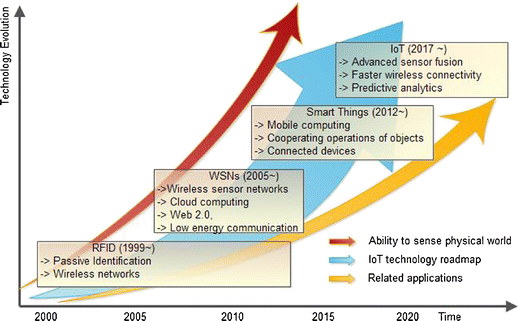
\includegraphics[width=0.85\textwidth]{iot-trend.png}
 \end{center}
 \caption{Evolution of the IoT and related technologies. (Source:~\protect\cite{li2015}) }
  \label{fig:iot-trend}
\end{figure}
%
By using sensor devices connected through networks, our awareness about the environmental conditions
increased significantly. Furthermore, sensor networks have opened
new horizons to make an assessment of the conditions of the
world at different levels, with the help of communication at the micro (even nano) and macro scales.
Without measurements, sustainable development effort can not progress in the right direction.
Especially precise measurements
from sensors are vital for the sustainable development of green systems. 
Wireless sensor networks are vital for monitoring in real time and making accurate measurements for such endeavor.
With the IoT (and especially
with sensor networks) not only energy statistics
can be collected but also numerical data that provide
information about the totality of the condition of the
earth can be acquired. Applications such as air pollution
control and measuring biodegradation can utilize sensors for making accurate measurements, for smarter and
greener world. Great financial savings can be made by utilizing sensor networks. The paper~\cite{rabaey2000} presents a 
striking example of the financial savings that can be made from the utilization of the WSNs:
%
%
\begin{quote}
\enquote{First-order estimations indicate that such technology could reduce
source energy consumption by two-quadrillion BTUs (British
Thermal Units) in the US alone. This translates to \$55 billion per
year, and 35 million metric tons of reduced carbon emissions.}
\end{quote}
\vspace{-5mm}
%
Just to give an idea about the diversity of application areas of WSN, the following short list can be given:
%
\begin{itemize} 
\setlength{\itemsep}{0.5pt}
\item {\bf Environmental:} Flood Detection, Forest Fire Detection, Air Pollution Monitoring
\item {\bf Household:} Water/Energy Metering/Monitoring, Remote Control, Security
\item {\bf Health:} Patient Monitoring
\item {\bf Industrial:} Monitoring Hazardous Gases, Quality Control
\item {\bf Agriculture-Farming:} Green House Control, Animal Tracking
\end{itemize} 
% 
% 
%
%
%%%%%%%%%%%%%%%%%%%%%%%%%%%%%%%%%%%%%%%%%%%%%%%%%%%%%%%%%%%%%%%%%%%%%%%%%%%%%%%%%%%%%%%%%%%%%%%%%%%%%%%%%%%%%%%%%%%%%%%%%%%%%
\newpage
\section{Sensor Nodes and Networks}\label{snodes}
%
Sensor nodes are basically small computers specialized on a certain task, namely sensing. Sometimes they can also "actuate" certain devices
through "wired medium" or through "wireless medium". The CPU part, generally, consists of very lightweight computing circuitry. 
Sensor node, which is generally called "mote", consists of processing unit, communication unit, power unit, and sensing unit. Optionally, 
motes may have a harvesting unit, mobilizer unit (for movement), and a location finding subsystem. These units can be seen in Figure~\ref{fig:parts-mote} below
in which important functional and structural elements of a generic mote are depicted. A real life example can be seen in
Figure~\ref{fig:typical-mote}. Mostly the modular structure enables motes to have various sensors and various communication units.
%

\vspace{2cm}
\begin{figure}[!htbp]
 \begin{center}
  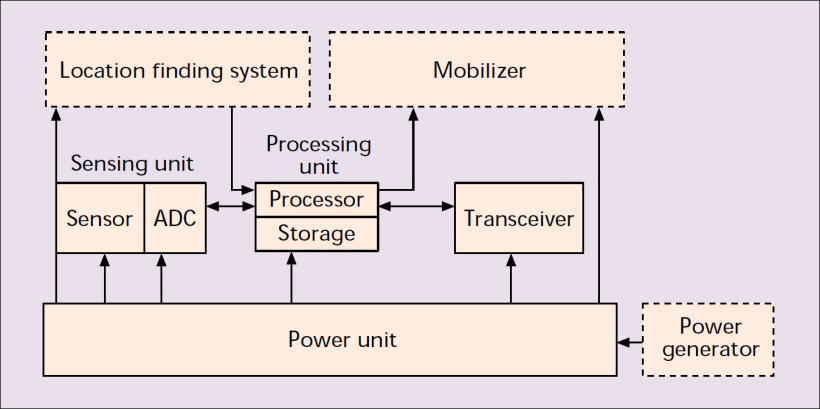
\includegraphics[width=0.85\textwidth]{wsn-arch2.png}
 \end{center}
 \caption{Components of a generic Sensor Node. Dotted lines is for optional elements. (Source:~\protect\cite{akyildiz2002}) }
  \label{fig:parts-mote}
\end{figure}
%

\begin{figure}[!htbp]
 \begin{center}
  \includegraphics[width=0.85\textwidth]{waspmote.jpg}
 \end{center}
 \caption{Typical Wireless Sensor Node. (Source: {\url{https://www.libelium.com/downloads/documentation/waspmote_datasheet.pdf}})  }
  \label{fig:typical-mote}
\end{figure}
%
% 
%

\newpage
In Table~\ref{tab:motes} specifications of several motes that are widely used are given. Motes generally have very lightweight CPUs with several kilobytes of memory.
The communication system supports very low bitrates for transmission, which is generally (as of 2018) around 250 kilobits per second. They also have lightweight OSs, 
like TinyOS (\url{http://www.tinyos.net/}) and Contiki (\url{http://www.contiki-os.org/}). Communication software stack is also lightweight and sometimes 
requiring "cross-layer"(\cite{sah2018}) optimizations. Cross-layer design is a new paradigm that is introduced for eliminating overheads that come from the standard 
design of the layered network. Taxonomy of the sensor nodes according to various criteria can be found in~\cite[pp.~81-84]{sohraby2007}.
%


\renewcommand{\arraystretch}{2}%
\begin{table}[H]
\begin{center}
\caption{Specifications of some widely used motes. (Source: Appendix A of~\cite{yang2014})}
\label{tab:motes}
\begin{adjustbox}{max width=\textwidth}
\begin{tabular}{| c || c | c | c | c | c | c |} 
\hline
\rowcolor{lightgray}
\textbf{Platform} & \textbf{CPU} & \textbf{Clock (MHz)} & \textbf{RAM/Flash/EEPROM} & \textbf{Radio Transceiver} & \textbf{BW (bps)} & \textbf{Freq. (MHz)}  \tabularnewline
\hline \hline   
 \cellcolor{lightgray} Telos  & TI MSP430F149     & 8 & 2K/60K/512K  & TI (Chipcon) CC2420 & 250k  & 2400 \tabularnewline \hline
 \cellcolor{lightgray} MicaZ  & Atmel Atmega 128L & 8 & 4K/128K      & TI (Chipcon) CC2420 & 250k  & 2400 \tabularnewline \hline
 \cellcolor{lightgray} Mica2  & Atmel Atmega 128L & 8 & 4K/128K/512K & TI (Chipcon) CC1000 & 38.4k & 900 \tabularnewline \hline
 \cellcolor{lightgray} Libelium Wasp mote &  Atmel ATMega1281 & 8 & 8K/128K/2GB & XBee\textsuperscript \textregistered module\tablefootnote{XBee\textsuperscript \textregistered is an IEEE 802.15.4 RF Module by Digi International:~\url{https://www.digi.com/}}  & 250/230/230k & 2400/900/848 \tabularnewline \hline
\end{tabular}
%\\[1.0] %You can adjust how far below the table the text should appear
\end{adjustbox}
\end{center}
\end{table}
\renewcommand{\arraystretch}{1}%

% 
%
% 
\newpage




For the networking of motes, important design choices and parameters come into play. Network subsystem including the radio module determines 
the way the communication proceeds. Designers should consider factors like the mobility of the nodes, antenna types and specifications, modulation techniques, routing protocols, 
transmission medium (air, water, human body), transmission frequency (which depends on the antenna, power requirements, range requirements, and transmission medium).
The physical network structure of the deployed nodes is called topology or topological structure. 
The topological structure of a WSN is also another important design element affecting performance and energy efficiency~\cite{fabian2009, kaur2012}. 
Generally, there are two basic types of nodes in most of the WSNs. Sensor nodes (motes) that are responsible for actual sensing and "sink" (base station) nodes that are 
collecting the sensory data from sensor nodes. Sink nodes generally have different architecture. They should basically have better power units.
In choosing topological structure designers can choose between hierarchical or non-hierarchical topologies. In the WSNs where nodes have mobility, the topology is 
not fixed. In this sense, these topologies are regarded as "static" type of topologies. MANETs are instances of mobile networks, in which devices can move.

In the case of static WSNs, following classification can be given for the widely used topologies:
\begin{itemize}
\item Hierarchical: Tree like topologies formed with multiple sink nodes.
\item Non-Hierarchical: Topologies with, generally, single sink node.
\begin{itemize}
\item Star
\item Mesh
\item Grid
\item Ring
\end{itemize}
\end{itemize}

Multiple sink nodes can be arranged in a "hierarchical" structures. In Figure~\ref{fig:mesh2} such topology example can be seen. In these type of topologies, 
multiple star, grid, or mesh topologies are connected in a recursive way. Consequently, multiple sink nodes are connected to a sink node at the higher level in the
hierarchy. 
% 
%
% 
\begin{figure}[!htbp]
\begin{center}
  %\includegraphics[width=5in]
  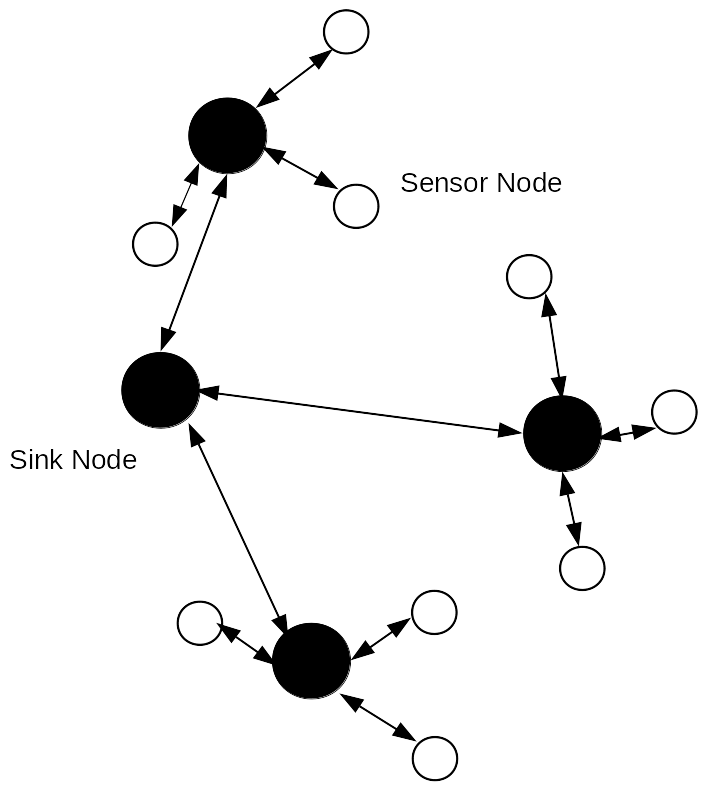
\includegraphics[width=0.5\textwidth]{mesh2.png}
   \end{center}
  \caption{Hierarchical Topology used in WSNs.}
 \label{fig:mesh2}
\end{figure}
% 
%
% 
% 

Star (Figure~\ref{fig:star}), mesh (Figure~\ref{fig:mesh}),
grid (Figure~\ref{fig:grid}), and  ring (Figure~\ref{fig:ring}) are examples of non-hierarchical topologies, 
in which there is a single sink node. 
In Figure~\ref{fig:mesh2}, and figures~\ref{fig:star}-\ref{fig:ring} arrows are depicting routing information. They are not representing wired connection.
% 
%
% 
\begin{figure}[!htbp]
  \begin{subfigure}[b]{0.45\textwidth}
    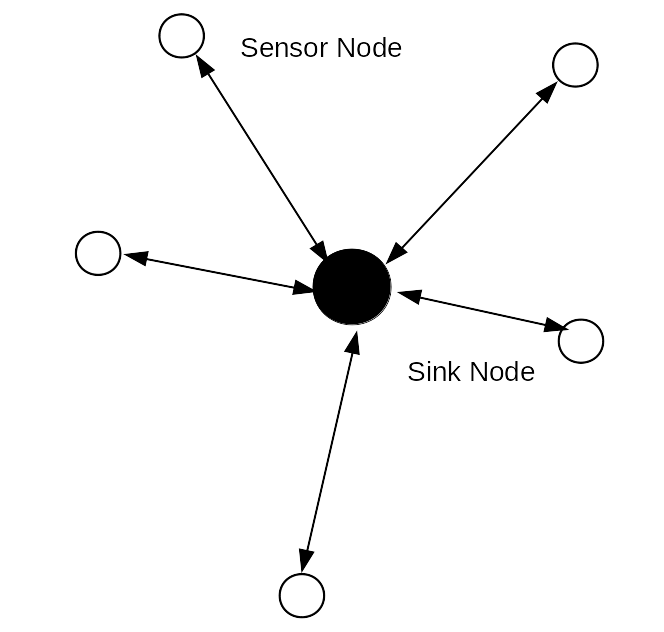
\includegraphics[width=\textwidth]{star.png}
    \caption{Star Topology.}
    \label{fig:star}
  \end{subfigure}
  \hfill
  \begin{subfigure}[b]{0.45\textwidth}
    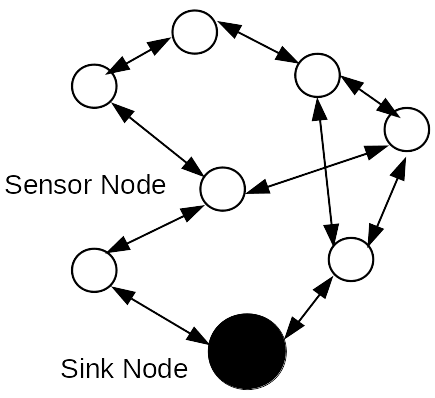
\includegraphics[width=\textwidth]{mesh.png}
    \caption{Mesh Topology.}
    \label{fig:mesh}
  \end{subfigure}
   
  \caption{Non-Hierarchical Topologies used in WSNs.}
\end{figure}
% 
%
% 

\newpage
% 
%
% 
\begin{figure}[!tbp]
  \begin{subfigure}[b]{0.4\textwidth}
    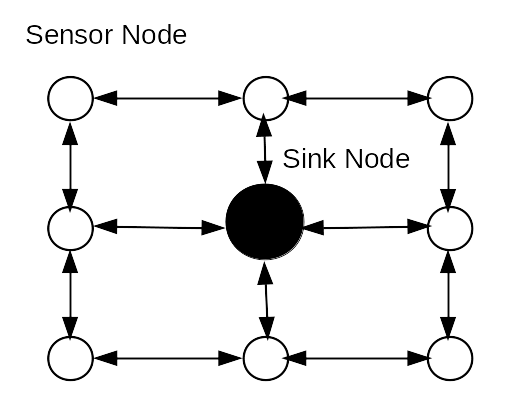
\includegraphics[width=\textwidth]{grid.png}
    \caption{Grid Topology.}
    \label{fig:grid}
  \end{subfigure}
  \hfill
  \begin{subfigure}[b]{0.4\textwidth}
    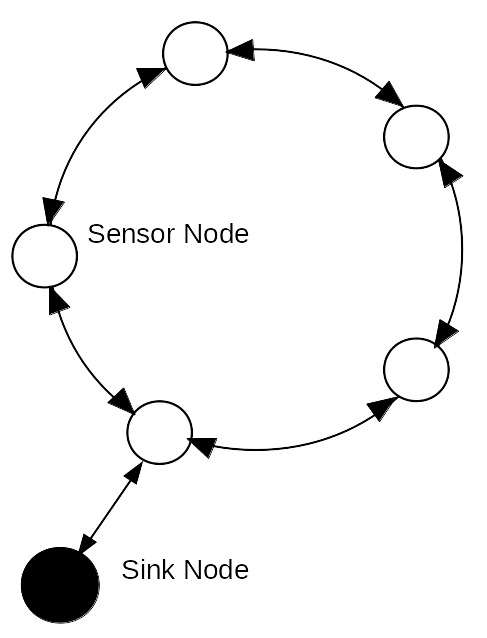
\includegraphics[width=\textwidth]{ring.png}
    \caption{Ring Topology.}
    \label{fig:ring}
  \end{subfigure}
  \caption{Non-Hierarchical Topologies used in WSNs.}
\end{figure}
% 
%














% 
% \newpage
% 
% 
%  
% \begin{figure}[!htbp]
% \begin{center}
%   %\includegraphics[width=5in]
%   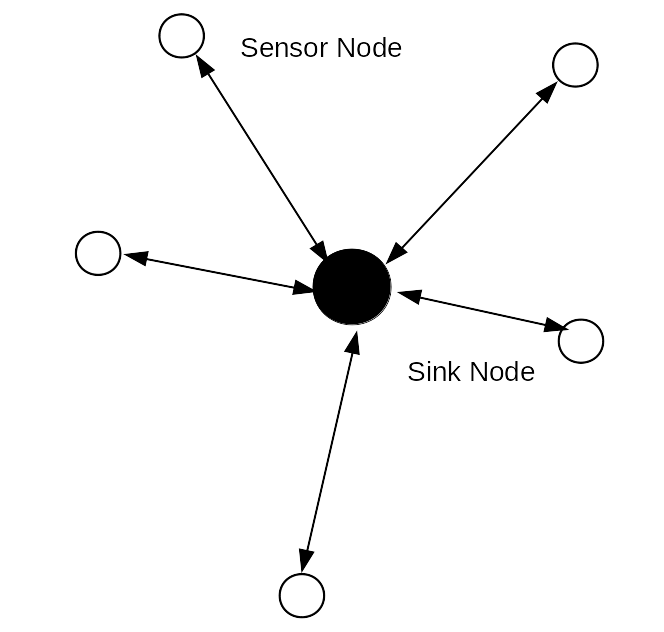
\includegraphics[width=0.7\textwidth]{star.png}
%   \hfill
%   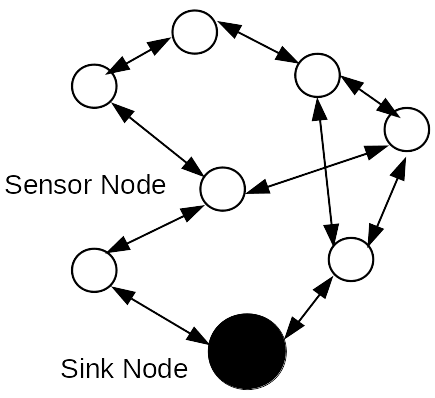
\includegraphics[width=0.5\textwidth]{mesh.png}
%    \end{center}
%   \caption{Star Topology}
%  \label{fig:star}
% \end{figure}
% 
%  
% \begin{figure}[!htbp]
% \begin{center}
%   %\includegraphics[width=5in]
%   
%    \end{center}
%   \caption{Mesh Topology}
%  \label{fig:mesh}
% \end{figure}
% 
% 
%  
% \begin{figure}[!htbp]
% \begin{center}
%   %\includegraphics[width=5in]
%   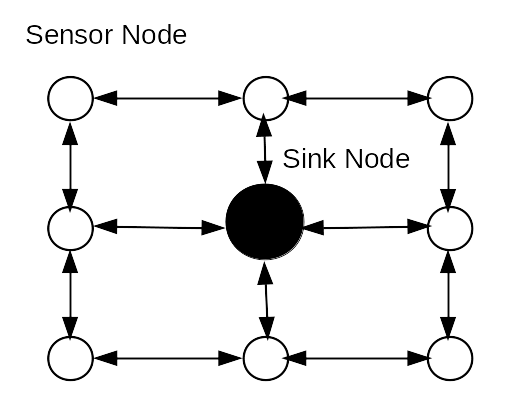
\includegraphics[width=0.5\textwidth]{grid.png}
%   \hfill
%    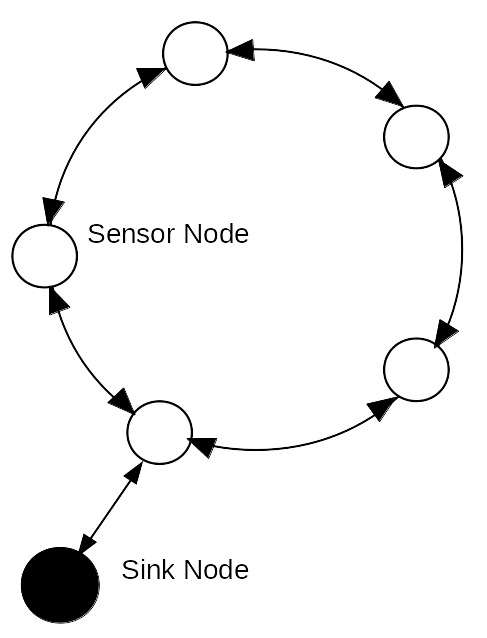
\includegraphics[width=0.5\textwidth]{ring.png}
%    \end{center}
%   \caption{Grid Topology}
%  \label{fig:grid}
% \end{figure}
% 
% 
%  
% \begin{figure}[!htbp]
% \begin{center}
%   %\includegraphics[width=5in]
%   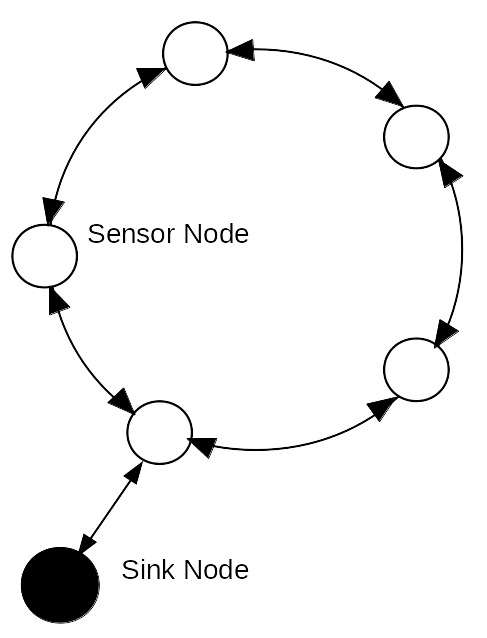
\includegraphics[width=0.5\textwidth]{ring.png}
%    \end{center}
%   \caption{Ring Topology}
%  \label{fig:ring}
% \end{figure}
% 
%
% 



%
%
%%%%%%%%%%%%%%%%%%%%%%%%%%%%%%%%%%%%%%%%%%%%%%%%%%%%%%%%%%%%%%%%%%%%%%%%%%%%%%%%%%%%%%%%%%%%%%%%%%%%%%%%%%%%%%%%%%%%%%%%%%%%%
%\chapter{System Models}\label{ssysmodel}

\newpage

In today's technology, nanosensors are utilized in various applications like biomedical, industrial, environmental, and military. 
With the networking technology, nanosensors, in general nanomachines, become more potent, since they can cooperate and 
communicate for achieving more challenging tasks. Figure~\ref{fig:arch}, shows the general network architecture to 
be assumed in this thesis for the targeted nanonetworks. 



% 
%
%

\begin{figure}[!htbp]
\begin{center}
  %\includegraphics[width=4in]
  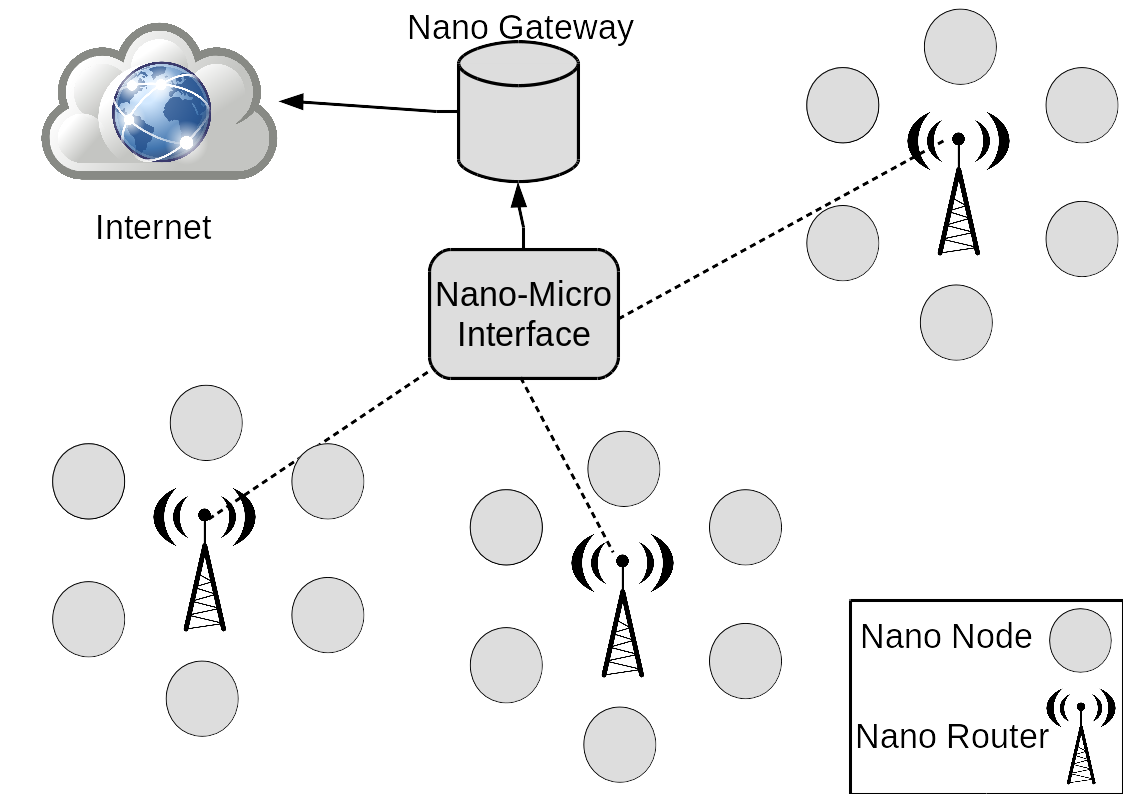
\includegraphics[width=0.65\textwidth]{myarch.png}
   \end{center}
  \caption{Network architecture and components for nanonetworks}
 \label{fig:arch}
\end{figure}
% 
%
%







WNSNs are not very much different than the WSNs when we consider the architecture of the system.
In Figure~\ref{fig:wsn-arch}, a typical multi-path WSN structure can be seen.
Important elements of the nanonetworks are nanonodes, 
nanorouters, and nanomicro interfaces. Through gateways, these type of networks can be connected to the traditional Internet.


\begin{figure}[!htbp]
\begin{center}
  %\includegraphics[width=4in]
  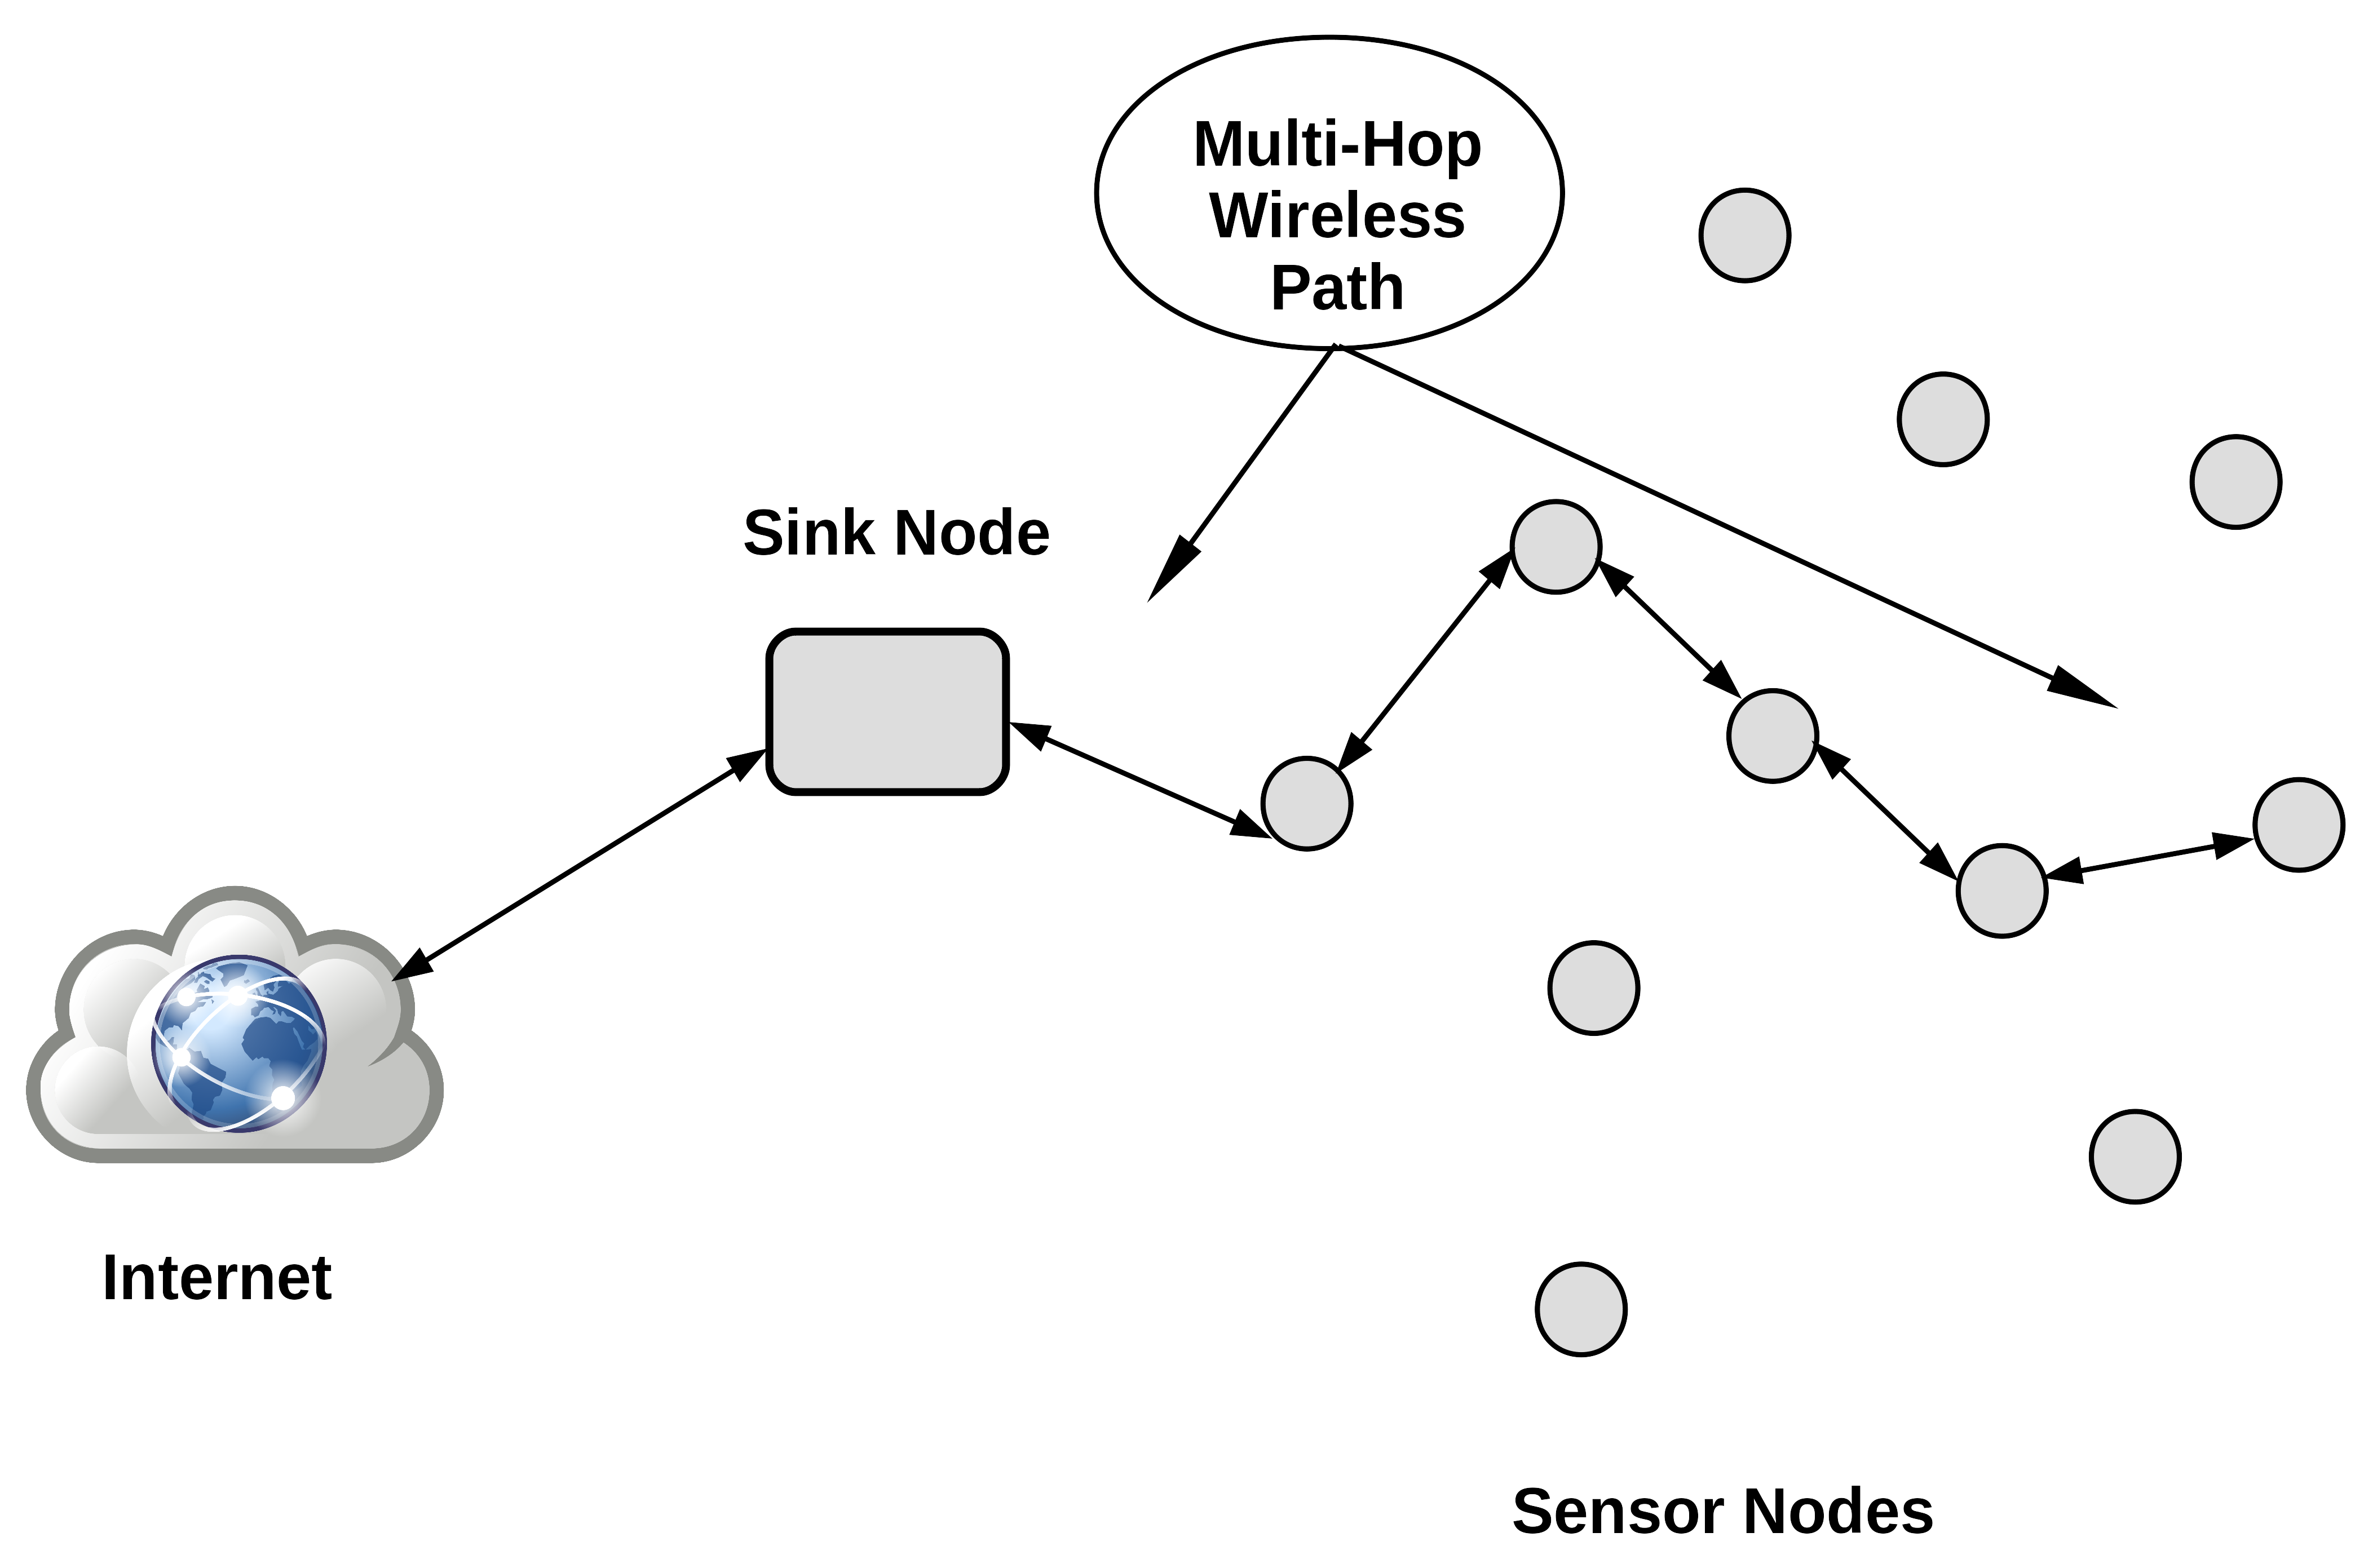
\includegraphics[width=0.7\textwidth]{wsn-graph.png}
    \end{center}
  \caption{Typical Wireless Sensor Network - WSN}
 \label{fig:wsn-arch}
\end{figure}

% 
%
%

The communication in nanonetworks can utilize one of the following technologies; nanomechanical, acoustic, electromagnetic and chemical or molecular communication~\cite{akyildiz2008}. A comparison for the existing communication technologies can be summarized as shown in Table~\ref{tab:techs}.
% 
%
%

\begin{table}[H]
\begin{center}
\caption{Comparison of communication technologies used in nanonetworks}
\label{tab:techs}
\begin{adjustbox}{max width=\textwidth}
\begin{tabular}{|c || L| L | L |} 
\hline
\rowcolor{lightgray}
\textbf{Comm. Type} & \textbf{Internet} & \textbf{Nano-Molecular} &\textbf{Nano-Wireless} \tabularnewline
\hline \hline
\cellcolor{lightgray} \textbf{Signal Type} & Electro-Magnetic & Chemical & Electro-Magnetic \tabularnewline  \hline
\cellcolor{lightgray} \textbf{Signal Speed} & High  & Low & High \tabularnewline \hline
\cellcolor{lightgray} \textbf{Power Consumption} & High & Low & Low \tabularnewline \hline 
\end{tabular}
%\\[1.0] %You can adjust how far below the table the text should appear
\end{adjustbox}
\end{center}
\end{table}
%\vspace{-1.0cm}
% 
%
%
Mainly due to their tiny sizes, nanonetworks introduce difficulties in both hardware and software design. Detailed explanations on the hardware design of the electromagnetic wireless nanosensors can be found in~\cite{akyildiz2010-2}. Especially for the software part,
the communication layer stack needs fine tuning as the hardware imposes many restrictions.
The physical signaling is at the THz levels, due to antenna size, requiring special modulation techniques~\cite{jornet2013-phd}. 
On the other hand, promising research is being done by using graphene based plasmonic materials for antennas to overcome signaling difficulties~\cite{jornet2013, jornet2013-phd}.
Nano scale batteries can not store much energy for the long duration of the nonstopping operations in the nanonodes.

The limitations that are listed in this section impose restrictions on the design of network communication layers. 
For the nanosensor nodes instead of regular TCP/IP protocol suite customized network stack has to be used, although there is no standard protocol stack for nanocommunication.
In~\cite{piroNS32013}, authors proposed a prototype protocol (layer) stack that is customized for nanosensor nodes. The proposed layer stack consists of four layers. 
These layers and their functions can be listed as follows:
\begin{itemize}
\item Message Process Unit: Generation and processing of messages.
\item Network layer: Routing of the packets.
\item Media access control entity: MAC layer without acknowledgments and retransmissions.
\item PHY (physical) interface: Modulation of the signals in THz band and bit transmission.
\end{itemize}
One of the best examples of the difficulties in software is the routing protocols for nanocommunication (overview on routing can be found in~\cite{neupane2014}). Considering the communication as being the most energy consuming operation for nanonodes, it is not difficult to see the importance of the "energy efficient" methods in communications. The energy cost of a routing protocol is high for a 
nanodevice and nanobatteries are very limited. In fact, the effectiveness of routing plays important role in energy efficient use of nanonetworks. Different from the traditional network routing protocols, nanorouting protocols have to be "energy-aware" optimization methods. Unlike the regular TCP/IP communication where devices can emit thousands of packets in seconds and the buffer memory is not a problem, in nano communication, only a few packets in a minute can be sent and the memory is limited. 

\newpage
Mostly because of the limitations in the current technology, any design on the nanotechnology has to follow a bottom-up approach. Structure of the system and the system element in 
nanoscales determine the design of the  higher level elements. This is shown in Figure~\ref{fig:design} (\cite{akyildiz2010-1}) below. Alternatively, innovative and nature-inspired ideas related to topology and fault tolerance in nanonetwork design can be found in~\cite{ilhan2016},~\cite{senel2011}, and in~\cite{imran2012}.

% 
%
%
\begin{figure}[!htbp]
\begin{center}
%\includegraphics[scale=0.35]
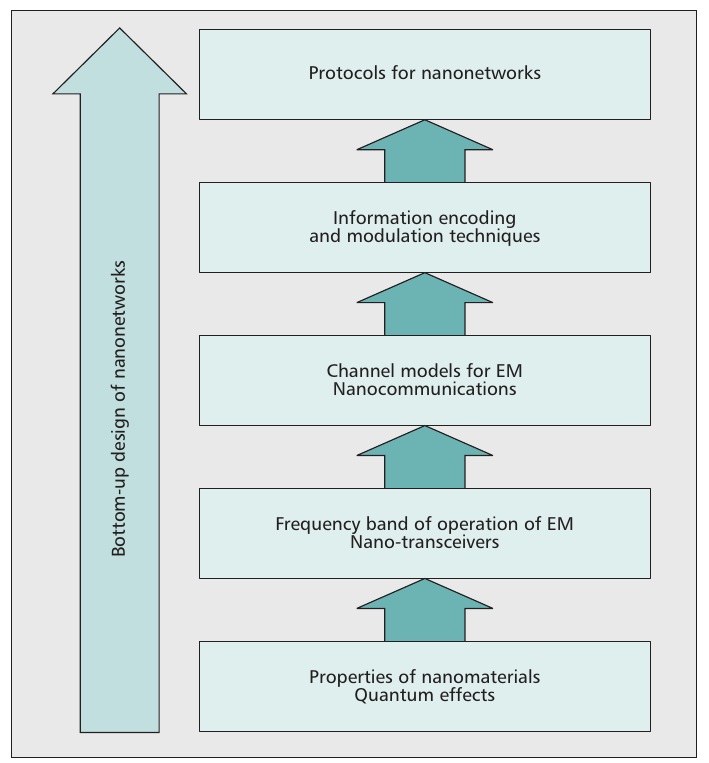
\includegraphics[width=0.8\textwidth]{design2.png}
  \end{center}
  \caption{Bottom-up Approach to the Design of Nano-networks. (Source: I. F. Akyildiz and J. M. Jornet, The Internet of nano-things~\protect\cite{akyildiz2010-1})}
 \label{fig:design}
\end{figure}
% 
%
%


\newpage
%%%%%%%%%%%%%%%%%%%%%%%%%%%%%%%%%%%%%%%%%%%%%%%%%%%%%%%%%%%%%%%%%%%%%%%%%%%%%%%%%%%%%%%%%%%%%%%%%%%%%%%%%%%%%%%%%%%%%%%%%%%%%
\section{Current Challenges}\label{scurrchal} 
As the new application areas are emerging for the use of sensors, the number of sensors is growing rapidly. 
Considering the industrial uses of sensors, a forecast can be seen from Figure~\ref{fig:forecast-wsn}, about 
the number of the industrial wireless sensors for the beginning of the 2020s. It is estimated that the number will reach 33 million by 2021.
% 
%
% 
\begin{figure}[!htbp]
\begin{center}
  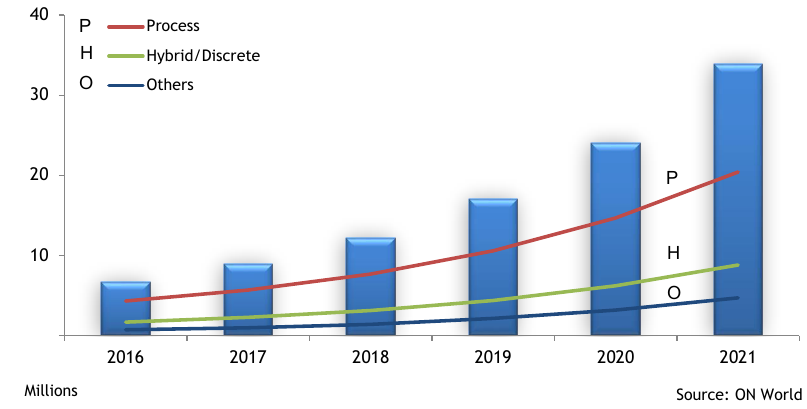
\includegraphics[width=0.8\textwidth]{global-wsn-devices2.png}
   \end{center}
  \caption{Global installed industrial WSN devices by market segment for 2016-2021. (Source: Industrial Wireless Sensor Networks~\protect\cite{ONworld2017})}
 \label{fig:forecast-wsn}
\end{figure}
% 
%
%

The number of devices or "things" connected to the Internet is also increasing rapidly. According to~\cite{regalado2014} the number of "things" 
(including all networked devices) will reach close to 30 billion by 2020s, as it can be seen in Figure~\ref{fig:mit-iot-forecast} below.
% 
%
%
\begin{figure}[!htbp]
\begin{center}
  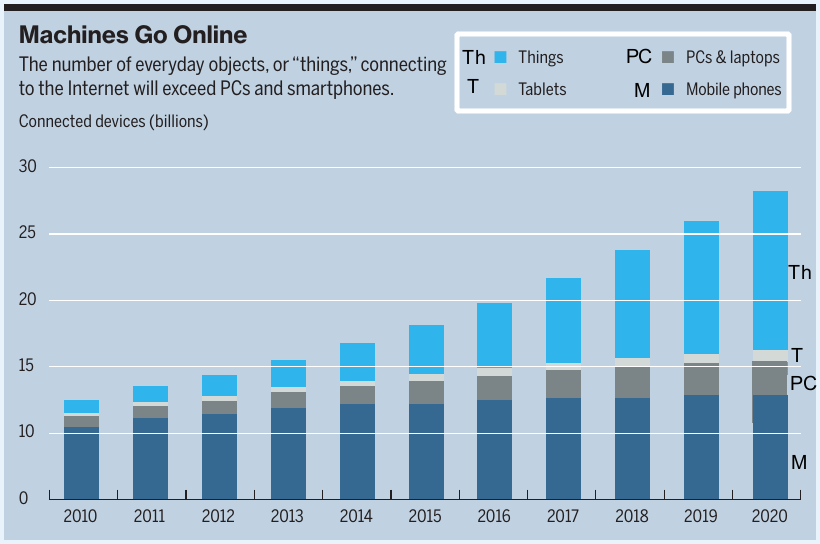
\includegraphics[width=0.65\textwidth]{mit-iot-forecast2.png}
   \end{center}
  \caption{Breakdown of the devices connected to the Internet. (Source:~\protect\cite{regalado2014})}
 \label{fig:mit-iot-forecast}
\end{figure}
% 
%
%
For practical uses of the sensors, the density of the sensor or other embedded networking devices, in a given unit space ($m^3$), 
can reach to a very high number. 
The cabling for such configurations may not be possible to realize. For this reason, such devices are mostly battery powered wireless devices 
that are designed to have maximized lifetime. 
In this sense, wireless communication is one of the peculiarities of the sensors.

Another peculiarity is the use of small batteries.
Sensors, being very small devices present ease of use. But their small scale footprint implies small scale energy unit.
For this reason, small energy storage in the sensors can be a bottleneck if the sensor networks and sensor nodes are not optimized
at the hardware level and at the software level. Generally, battery replacement is difficult due to the number of sensors nodes, 
and the cost of the labor for replacing batteries can be a major issue~\cite{callaway2004}.
Maximizing lifetime of the sensor nodes is essential in order to reduce the maintenance of this devices~\cite[p.~13]{shelby2010}.
Even some times due to the difficulties in reaching the sensor node, battery replacement is not an option. For example, in leakage detection sensor systems, sensors can be 
placed several meters under the ground, making it difficult to do any wireless recharging or perform battery replacement.
Energy harvesting is another technology that can be utilized for overcoming limited energy on the sensor nodes. 
A comprehensive review on the harvesting technologies for the sustainable use of the WSNs can be found in~\cite{panda2010, akbari2014, panatik2016, shaikh2016}.
On the other hand, according to~\cite{thiele2018} not only the battery capacity is growing slowly, but also harvesting technologies are 
limited because of the available low energy density. In~\cite{ditzel2007}, a similar argument on the power demand of the consumers 
and slow pace of the development of the battery technology to keep up with this demand is presented. 
Table~\ref{tab:harvesting-sources} presents a comparison of some harvesting sources.


\renewcommand{\arraystretch}{1}%
\begin{table}[H]
\begin{center}
\caption{Comparison of energy harvesting sources. (Source:~\cite{akbari2014})}
\label{tab:harvesting-sources}
\begin{adjustbox}{max width=\textwidth}
\begin{tabular}{| >{\centering}m{3cm} | >{\centering}m{3cm} | >{\centering}m{3cm} | >{\centering}m{4cm} |}
\hline
\rowcolor{lightgray}
\textbf{Energy Source} & \textbf{Conditions} & \textbf{Performance} & \textbf{Surface or volume providing energy of an AA} \tabularnewline
\hline \hline
Solar     & Outdoors &  \SI{7500}{\micro\watt}$/cm^2$  &  23x23$/cm^2$    \tabularnewline \hline
Solar     & Indoors  &  \SI{100}{\micro\watt}$/cm^2$   &  198x198$/cm^2$  \tabularnewline \hline
Vibration & 1$m/s^2$ &  \SI{100}{\micro\watt}$/cm^3$   &  34x34x34$/cm^3$ \tabularnewline \hline 
RF        & WiFi     &  \SI{0.001}{\micro\watt}$/cm^2$ &  625x625$/m^2$   \tabularnewline \hline
RF        & GSM      &  \SI{0.1}{\micro\watt}$/cm^2$   &  62x62$/m^2$     \tabularnewline \hline
\end{tabular}
%\\[1.0] %You can adjust how far below the table the text should appear
\end{adjustbox}
\end{center}
\end{table}
\renewcommand{\arraystretch}{1}%
% 
%
%
According to~\cite{knight2008, energizere91}, AA type alkaline batteries (E91 - 1.5V) can provide~\SI{2850}{\milli\ampere} from~\SI{8.3}{cm^3} volume, which is~\SI{3.90}{\watt\hour} 
maximum energy at nominal voltage and for~\SI{50}{\milli\ampere} drain~\cite{wiki-batteries}.
Taking this as a reference, the last column of Table~\ref{tab:harvesting-sources} is elaborated by estimating surface or volume required to provide the same amount of power that an AA type alkaline battery can provide. 
 
As of the year 2018, the AA type batteries are widely used in sensor nodes. 
This type of batteries are low cost, and widely available.
They are suitable for low current drawing applications at room temperature. But there are two disadvantages in using this type of batteries. 
The first is that, they do not perform well in the cold. So in cold and under high current draw, their capacity decreases sharply as it can be seen from the curves in
Figure~\ref{fig:e91}.
% 
%
%
\vspace{2cm}
\begin{figure}[!htbp]
\begin{center}
  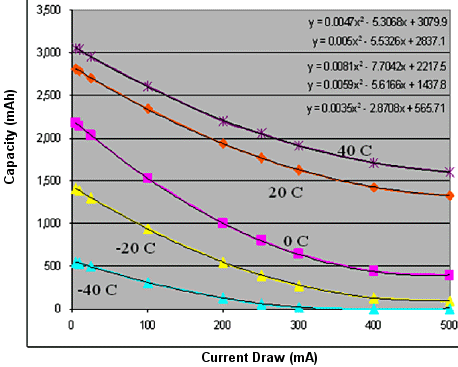
\includegraphics[width=0.90\textwidth]{e91.png}
   \end{center}
  \caption{Temperature current model of an alkaline AA (E91 - 1.5V) battery. (Source:~\protect\cite{young2008})}
 \label{fig:e91}
\end{figure}
% 
%
%

\newpage

The second drawback is that, under high current draw they do not perform well. 
Figure~\ref{fig:alkaline} depicts the comparison of the performances of various types of batteries in two modes. Namely, they are labeled as "Rated" and "Actual". 
"Rated" mode is related to the specific energy while the battery is discharging at a very low current.
"Actual" mode specifies discharges at 1 Coulomb, which is the general way that batteries are rated. In the case of "Actual" mode, the performance of alkaline batteries drops as it is shown.
%\vspace{-1cm}
% 
%
%
\begin{figure}[!htbp]
\begin{center}
  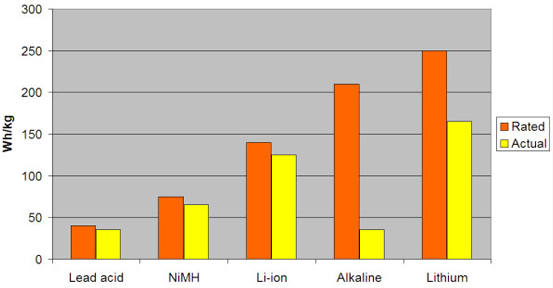
\includegraphics[width=0.85\textwidth]{alkaline.png}
   \end{center}
  \caption{Battery comparison. Because of the high internal resistance, alkaline battery performance degrades under high current draw. 
(Source:~\protect\url{https://batteryuniversity.com/learn/article/primary_batteries})}
 \label{fig:alkaline}
\end{figure}
% 
%
%

Considering the use of Mica2 sensor node for measuring temperature every minute with 128 bytes data packets (Zigbee protocol\footnote{Zigbee is an IEEE 802.15.4 based specification for high-level communication protocols developed by Zigbee Alliance~\url{http://www.zigbee.org/}} allows max packet size of 133 bytes), at 38.4Kbps (1 kilobit = 1024 bits) rough estimate for each 
transmission can be given with the equation~\ref{eq:trans} below:
\begin{equation}
(128 \times 8) / (38.4 \times 1024)~=~\SI{0.02604}{\secs}~=~\SI{26.04}{\milli\secs} \label{eq:trans}
\end{equation}
% 
%
%
For a rough estimate, the inclusion of the control signals like positive and negative acknowledgments (ACK and NACK) as extra packets and wake up time of~\SI{0.18}{\milli\secs}~\cite{polastre2005}, will make transmission time about~\SI{50}{\milli\secs} (overestimation). The rest of the time it is assumed that the sensor node is in "sleeping state". In this sense, "awake time" and "sleep time" is given in equations~\ref{eq:awake} and in~\ref{eq:sleep} below:
\begin{gather}
\text{Awake Time per day}~=~24 \times 60 \times \SI{0.05}{\secs}~=~\SI{72}{\secs}~=~\SI{0.02}{\hour} \label{eq:awake} \\
\text{Sleep Time per day}~=~24 \times 60 \times 60 – \SI{72}{\secs} ~=~ \SI{86328}{\secs}~=~\SI{23.98}{\hour} \label{eq:sleep}
\end{gather}
% 
%
%
According to Mica2 datasheet\footnote {\url{http://www.investigacion.frc.utn.edu.ar/sensores/Equipamiento/Wireless/MICA2_Datasheet.pdf}} sleep current is about~\SI{15}{\micro\ampere} 
and the wake-up, transmission, and CPU currents, for an overestimation, can be summed up as~\SI{50}{\milli\ampere}. According to~\cite{bazzi2015}, Mica2 node consumes maximum~\SI{27}{\milli\ampere}
on transmission and~\SI{10}{\milli\ampere} in average for receiving. With some additional sensor board, the overestimation offered can be regarded rather realistic.
Then energy requirement for~\SI{24}{\hour} in~\SI{}{\milli\ampere\hour} can be given in equation~\ref{eq:daily} and  the average daily 
current draw is given in equation~\ref{eq:average}:
\begin{gather}
\text{Energy for~\SI{24}{\hour}}~=~(\SI{15}{\micro\ampere})\times(\SI{23.98}{\hour}) + (\SI{50}{\milli\ampere})\times(\SI{0.02}{\hour})~=~\SI{1.36}{\milli\ampere\hour}\label{eq:daily}\\
\text{Average Current}~=~\SI{1.36}{\milli\ampere\hour} / \SI{24}{\hour}~=~\SI{56.67}{\micro\ampere}~=~\SI{0.05667}{\milli\ampere} \label{eq:average}
\end{gather}
% 
%
%


Taking the rough estimates in the previous paragraphs as a reference, in Table~\ref{tab:e91}, the capacity of an AA size alkaline battery is 
listed under current draw of~\SI{0.05667}{\milli\ampere} for sensing temperature every minute
with the Mica2 sensor node in various temperature conditions.

\renewcommand{\arraystretch}{1.3}%
\begin{table}[H]
\begin{center}
\caption{Calculating capacity under~\SI{0.05667}{\milli\ampere} current draw of an Alkaline Model (E91 - AA) at different temperatures. 
$i$ represents current draw in~\SI{}{\milli\ampere}. (Source:~\cite{young2008})}
\label{tab:e91}
\begin{adjustbox}{max width=\textwidth}
\begin{tabular}{| >{\centering}m{4cm} | >{\centering}m{3cm} | >{\centering}m{5cm} | >{\centering}m{3cm} |}
\hline
\rowcolor{lightgray}
\textbf{Temperature (\SI{}{\celsius})} & \textbf{Capacity (mAh)} & \textbf{Output measured in~\SI{}{\milli\ampere\hour}} &  \textbf{Number of days Mica2 can be sustained} \tabularnewline
\hline \hline
\SI{40}{\celsius}  &    3080   &  0.0047 $i^2$– 5.3068 $i$ + 3079.9     &  2265  \tabularnewline \hline
\SI{20}{\celsius}  &    2837   &  0.005  $i^2$ – 5.5326 $i$ + 2837.1     &  2086  \tabularnewline \hline
\SI{0}{\celsius}   &    2218   &  0.0081 $i^2$ – 7.7042 $i$ + 2217.5    &  1631  \tabularnewline \hline
\SI{-20}{\celsius} &    1438   &  0.0059 $i^2$ – 5.6166 $i$ + 1437.8    &  1057  \tabularnewline \hline
\SI{-40}{\celsius} &    566    &  0.0035 $i^2$ – 2.8708 $i$ + 565.71    &   416  \tabularnewline \hline
\end{tabular}
%\\[1.0] %You can adjust how far below the table the text should appear
\end{adjustbox}
\end{center}
\end{table}
\renewcommand{\arraystretch}{1}%
% 
%
%
By using the data in Table~\ref{tab:e91} number of days that the Mica2 sensor node can be sustained at~\SI{20}{\celsius} is calculated as in the equation~\ref{eq:days} below:
\begin{equation}
\SI{2837}{\milli\ampere\hour} / ~\SI{1.36}{\milli\ampere\hour}~=~\SI{2086}{\days}~=~\SI{5.7}{\years} \label{eq:days}
\end{equation}
% 
%
%
The same calculations can be repeated for sensing temperature every second (almost real-time). 
The daily energy requirement can be found as~\SI{60.34}{\milli\ampere\hour} and the average current draw for each day can be found as~\SI{2.51}{\milli\ampere}. 
With these values, equation~\ref{eq:days2} can be used to find the number of days that the Mica2 sensor node can be sustained at~\SI{20}{\celsius} as:
\begin{equation}
\SI{2823}{\milli\ampere\hour} / ~\SI{60.342}{\milli\ampere\hour}~=~\SI{47}{\days} \label{eq:days2}
\end{equation}
% 
%
%


The estimates and the tables that are presented above are rough estimates and they are subjected to change over time with new and better technologies. 
On the other hand, they are presented to depict the situation of the energy management issues related to the WSNs numerically. 
Although harvesting technologies are vital for sensor nodes, currently they can not 
provide enough sustainability. However, in the long run, they should be improved to provide sustainable operation for WSNs. This does not mean to eliminate
research in the energy optimization. Currently, because of these power related issues, there is a growing research effort in the optimization of the energy consumption related
methods. Studies are focusing on the hardware and software optimization techniques.
In~\cite{anastasi2009}, a comprehensive and 
systematic taxonomy of the energy conservation schemes for the WSNs is presented. Limitations in the power supply units are not the only reasons that fuels the research in
energy optimization techniques. Analysis had shown that most of the energy is 
consumed by the communication module of the motes. Example breakdown of the power consumption can be seen in Figure~\ref{fig:power-cons}.
% 
%
%
\begin{figure}[!htbp]
 \begin{center}
  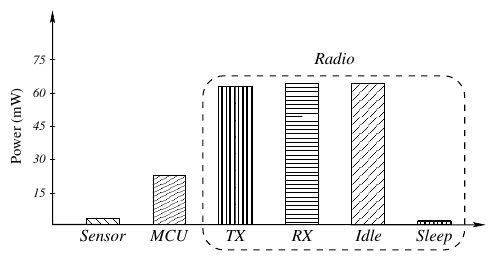
\includegraphics[width=0.75\textwidth]{power-cons.png}
 \end{center}
 \caption{A breakdown of the power consumption of a MicaZ sensor node. (Source: p. 44 of~\protect\cite{akyildiz2010-3})}
  \label{fig:power-cons}
\end{figure}
% 
%
%
\newpage


A similar comparison can be expressed in a quantitative way by quoting from~\cite{zhao2003}:
\begin{quote}
\enquote{For the Sensoria sensors and Berkeley motes, the ratio of energy
consumption for communication and computation is in the
range of 1000–10000.}
\end{quote}
%\vspace{-5mm}
% 
%
%


The Mica2\textsuperscript \textregistered\footnote{Mica2\textsuperscript \textregistered~\url{http://www.investigacion.frc.utn.edu.ar/sensores/Equipamiento/Wireless/MICA2_Datasheet.pdf} and MicaZ\textsuperscript \textregistered~\url{http://www.cmt-gmbh.de/MICAz.pdf} are sensor nodes produced by CrossBow~\url{http://xbow.com/}} 
mote can be seen in Figure~\ref{fig:mica2}. Compared to MicaZ\textsuperscript \textregistered, which transmits at 2.4GHz, Mica2 transmits at 900 MHz.
% 
%
%
\begin{figure}[!htbp]
 \begin{center}
  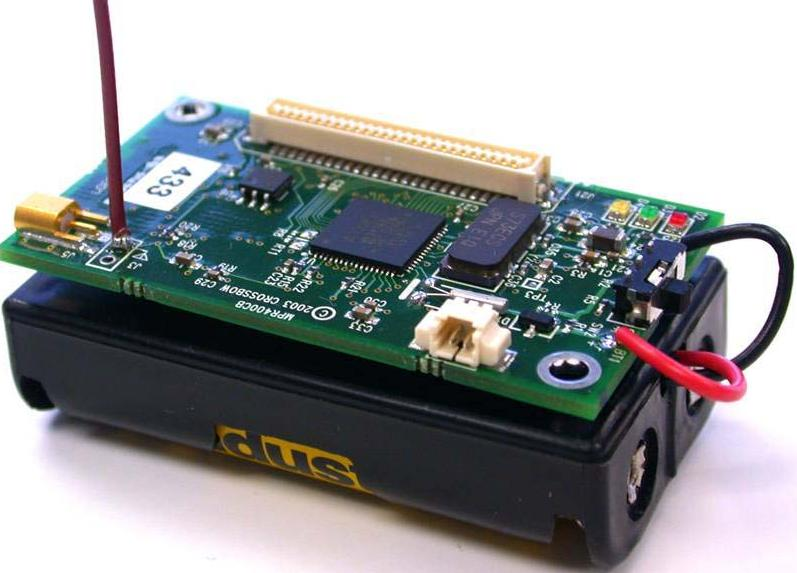
\includegraphics[width=0.45\textwidth]{mica2.jpg}
 \end{center}
 \caption{Picture of Mica2 sensor node. (Source:~\protect\url{http://www.snm.ethz.ch/snmwiki/pub/uploads/Projects/mica2.jpg})}
  \label{fig:mica2}
\end{figure}
% 
%
% 
Similar to Figure~\ref{fig:power-cons}, in which MicaZ power consumption comparison is given, in Figure~\ref{fig:mica2-power-cons}, 
the comparison of various power consuming events can be seen. In the figure, measured current draw for transmission is compared to other events.
% 
%
%
\begin{figure}[!htbp]
 \begin{center}
  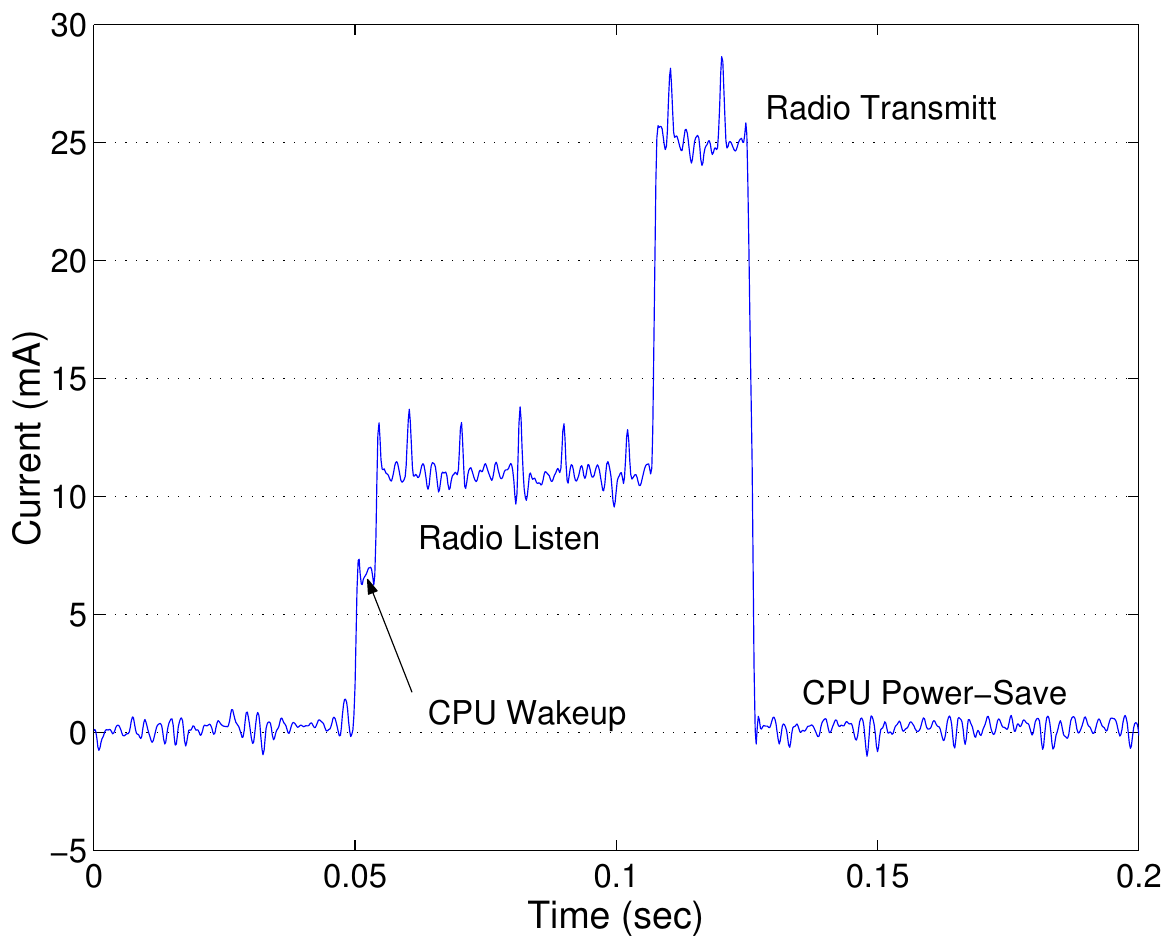
\includegraphics[width=0.5\textwidth]{mica2-power-graph.png}
 \end{center}
 \caption{Power consumption graph of Mica2 sensor node. (Source:~\cite{shnayder2004}\protect\footnotemark)}
  \label{fig:mica2-power-cons}
\end{figure}
\footnotetext{\protect\url{https://www.eecs.harvard.edu/~shnayder/ptossim/mica2bench/img/radio_scope.pdf}}
% 
%
%

\newpage
Table~\ref{tab:mica2-pow-cons} summarizes power model of the Mica2 mote by considering CPU and Radio
current draw.
 
\renewcommand{\arraystretch}{1}%
\begin{table}[H]
\begin{center}
\caption{Power model for Mica2 mote, with micasb sensor board and 3V power supply. (Source:~\cite{shnayder2004})}
\label{tab:mica2-pow-cons}
\begin{adjustbox}{width=\textwidth}
\begin{tabular}{| c | c |} 
\hline
\rowcolor{lightgray}
\textbf{CPU Modes} & \textbf{Current}  \tabularnewline
\hline \hline
Active                 &    \SI{8.0}{\milli\ampere}    \tabularnewline \hline
Idle                   &    \SI{3.2}{\milli\ampere}    \tabularnewline \hline
ADC Noise Reduce       &    \SI{1.0}{\milli\ampere}    \tabularnewline \hline
Power-down             &    \SI{103}{\micro\ampere}   \tabularnewline \hline
Power-save             &    \SI{110}{\micro\ampere}   \tabularnewline \hline
Standby                &    \SI{216}{\micro\ampere}   \tabularnewline \hline
Extended Standby       &    \SI{223}{\micro\ampere}   \tabularnewline \hline
Internal Oscillator    &    \SI{0.93}{\milli\ampere}   \tabularnewline \hline
LEDs                   &    \SI{2.2}{\milli\ampere}    \tabularnewline \hline
Sensor board           &    \SI{0.7}{\milli\ampere}    \tabularnewline \hline
\end{tabular}
\hspace{5mm}
\begin{tabular}{| c | c |} 
\hline 
\rowcolor{lightgray}
\textbf{EEPROM access} & \textbf{Current}  \tabularnewline
\hline \hline
Read            &    \SI{6.2}{\milli\ampere}       \tabularnewline \hline
Read Time       &    \SI{565}{\micro\secs}        \tabularnewline \hline
Write           &    \SI{18.4}{\milli\ampere}      \tabularnewline \hline
Write Time      &    \SI{12.9}{\milli\secs}        \tabularnewline \hline
\end{tabular}
\hspace{5mm}
\begin{tabular}{| c | c |} 
\hline 
\rowcolor{lightgray}
\textbf{Radio Modes} & \textbf{Current}  \tabularnewline
\hline \hline
Rx                &   \SI{7.0}{\milli\ampere}      \tabularnewline \hline
Tx (-20dBm)      &   \SI{3.7}{\milli\ampere}      \tabularnewline \hline
Tx (-19dBm)      &   \SI{5.2}{\milli\ampere}      \tabularnewline \hline
Tx (-15dBm)      &   \SI{5.4}{\milli\ampere}      \tabularnewline \hline
Tx (-8dBm)       &   \SI{6.5}{\milli\ampere}      \tabularnewline \hline
Tx (-5dBm)       &   \SI{7.1}{\milli\ampere}      \tabularnewline \hline
Tx (0dBm)        &   \SI{8.5}{\milli\ampere}      \tabularnewline \hline
Tx (+4dBm)       &   \SI{11.6}{\milli\ampere}     \tabularnewline \hline
Tx (+6dBm)       &   \SI{13.8}{\milli\ampere}     \tabularnewline \hline
Tx (+8dBm)       &   \SI{17.4}{\milli\ampere}     \tabularnewline \hline
Tx (+10dBm)      &   \SI{21.5}{\milli\ampere}     \tabularnewline \hline
\end{tabular}
%\\[1.0] %You can adjust how far below the table the text should appear
\end{adjustbox}
\end{center}
\end{table}
\renewcommand{\arraystretch}{1}%
% 
%
%
Considering the current limitations of the harvesting technologies and the current battery performances along with the 
high power consumption of the communication subsystem of the sensor nodes, it is necessary to do research for finding energy 
optimization methods related to the communication subsystem. Saving from the energy can always be used in other ways to increase
the effectiveness, robustness, and longevity of the WSN.
In this sense, the HW and SW optimization techniques are very much focused on the communication substructure of the motes, 
compared to the research on energy harvesting and on efficient power unit design~\cite{bomnale2018}.
% 
%
%
%Online rfc bib enrty creator: 
%http://notesofaprogrammer.blogspot.com/2014/11/bibtex-entries-for-ietf-rfcs-and.html
% 
%
%

%%%%%%%%%%%%%%%%%%%%%%%%%%%%%%%%%%%%%%%%%%%%%%%%%%%%%%%%%%%%%%%%%%%%%%%%%%%%%%%%%%%%%%%%%%%%%%%%%%%%%%%%%%%%%%%%%%%%%%%%%%%%%
\newpage
\section{Energy Optimization Techniques in WSNs}\label{senergy-opt}
While many research studies agree upon the energy problem in WSNs, designing a sustainable WSN requires interdisciplinary collaboration, 
as it involves expertise in SW, HW, electric circuitry, electromagnetics, electronics, and statistics. 
This does not mean that an expert in one of those fields listed can not offer a sustainable solution for the energy usage in WSNs. While the trade-offs are in play as in every 
optimization problem, very specialized optimization can not be very effective if any possible synergy is ignored. The basic idea is to prolong the network lifetime. 
Sometimes this goal may conflict with the QoS requirements. The extending lifetime may bring the cost of longer delay in transmissions. 
On the other hand, different lifetime criteria and definitions exist. In some specific application areas of WSNs, the network may die when the first node is out of batteries (dies), 
and in some when all the nodes die. 
With these caveats in mind, energy optimization techniques
in the literature should be carefully analyzed. In fact, authors in~\cite{rault2014} has mentioned one of the similar issues related to trade-offs, in which they argued that
optimization techniques proposed so far are not "universally applicable". The main idea in the paper~\cite{rault2014} is to optimize according 
to the application requirements of the WSNs. Authors listed five different application areas and seven different requirements specific to these application areas of the WSNs which can be seen in Table~\ref{tab:reqs}. The paper proposes these requirements as conditions that the energy optimization techniques should satisfy.

\renewcommand{\arraystretch}{1.5}%
\begin{table}[H]
\begin{center}
\caption{Applications and their requirements for WSNs. VL=Very Low, L=Low, H=High, VH=Very High. (Source:~\protect\cite{rault2014})}
\label{tab:reqs}
\begin{adjustbox}{max width=\textwidth}
\begin{tabular}{| l | l | c | c | c | c | c | c | c |} 
\hline
\rowcolor{lightgray}
\textbf{Application} & \textbf{Example} & \textbf{Scalability} & \textbf{Coverage} & \textbf{RT Delay} & \textbf{QoS} & \textbf{Security} & \textbf{Mobility} & \textbf{Robustness} 
\tabularnewline
\hline \hline


\multirow{2}{3cm}{Healthcare}                             &    Vital status monitoring    & VL   & VL  & VH  & H  & VH  &  VH  &  H \tabularnewline \hhline{~|-|-|-|-|-|-|-|-|}
                                                          &    Remote surveillance        & VL   & VL  & H   & H  & VH  &  VH  &  L \tabularnewline \hline  
\multirow{3}{3cm}{Agriculture \\ and environment}         &    Precision agriculture      & VH   & VH  & VL  & VL & VL  &  VL  &  H \tabularnewline \hhline{~|-|-|-|-|-|-|-|-|}
                                                          &    Cattle monitoring          & VH   & L   & L   & VL & VL  &  H   &  L \tabularnewline \hhline{~|-|-|-|-|-|-|-|-|} 
                                                          &    Environment monitoring     & VL   & VL  & H   & H  & VH  &  VH  &  L \tabularnewline \hline  
\multirow{2}{3cm}{Public safety and \\ military systems}  &    Active intervention        & VL   & VL  & VH  & H  & VH  &  VH  &  VH \tabularnewline \hhline{~|-|-|-|-|-|-|-|-|} 
                                                          &    Passive supervision        & VL   & H   & VH  & H  & VH  &  VL  &  L \tabularnewline \hline                 
\multirow{3}{3cm}{Transportation \\ systems}              &    Traffic control            & VL   & L  & VH  & VH  & VH  & VH   & L \tabularnewline \hhline{~|-|-|-|-|-|-|-|-|} 
                                                          &    Safety system              & VL   & L  & VH  & VH  & VH  & H    & H \tabularnewline \hhline{~|-|-|-|-|-|-|-|-|} 
                                                          &    Services                   & VL   & VL & L   &  H  &  H  & H    & L \tabularnewline \hline  
\multirow{2}{3cm}{Industry}                               &    SCADA systems              &  VL  & L  & VH  &  H  & VH  & VL   & VH \tabularnewline \hhline{~|-|-|-|-|-|-|-|-|} 
                                                          &    Smart grids                &  H   & L  & VH  &  H  & VH  & VL   & VH \tabularnewline \hline
\end{tabular}
%\\[1.0] %You can adjust how far below the table the text should appear
\end{adjustbox}
\end{center}
\end{table}
\renewcommand{\arraystretch}{1}%
% 


The paper presents an extensive classification of the energy efficient mechanisms specific to battery operated WSNs, which can be seen in Figure~\ref{fig:energy-opt-techs}.

% 
%
%
\begin{figure}[!htbp]
 \begin{center}
  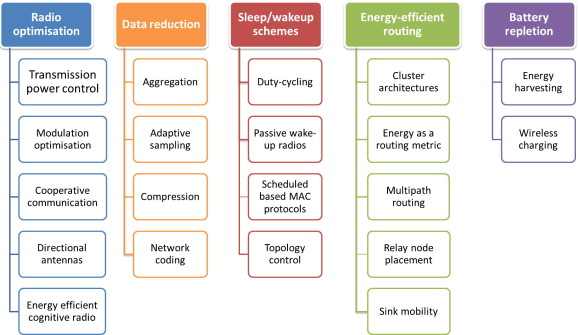
\includegraphics[width=0.90\textwidth]{energy-opt-techs.png}
 \end{center}
 \caption{The classification of the energy efficient mechanism used in WSNs. (Source:~\protect\cite{rault2014})}
  \label{fig:energy-opt-techs}
\end{figure}
% 
%
%
Authors in~\cite{rault2014} also provide discussions and give a comprehensive analysis of the effects of these techniques on the performance of the applications.
Case studies are included to show how trade-offs between multiple requirements can be handled for designing efficient and sustainable WSNs.

In~\cite{anastasi2009}, authors focused mostly on sensor node architecture and gave a taxonomy of energy conservation schemes. Their classification basically involves three classes of
energy conservation schemes, namely duty cycling, data-driven, and mobility based schemes. Duty cycling is an effective OS and HW level optimization technique, in which the components
can cycle between various levels of "SLEEP" and "WAKEUP" states. The idea is to put the components into "SLEEP" state when they are not needed and change the state to "WAKEUP" when
they are needed. The data-driven schemes build a statistical model of the sensed data for reducing the actual "sensing" activities with the "prediction". The idea in mobility based schemes
is to equip some or all nodes with mobility when the energy cost of mobility can be used to further reduce the communication energy cost.

Clustering is one of the optimization techniques that is offered for efficient energy usage (both network level and sensor level) and for "data
aggregation" (prevents data duplication). While the topology of the WSN is "clustered logically" introducing hierarchy, the transmission flow is also
controlled by elected "Cluster Heads" (CH). Various algorithms are proposed for the "election process" of the CHs, which is a crucial process for
energy optimization. The main idea is "balancing" the energy usage of the clusters and increasing the lifetime of the network~\cite{boyinbode2010}. The next phase is
the cluster formation, in which nodes based on some heuristics decide to join to a certain CH for forming a cluster.
Clustering is very extensively researched for the past twenty years. The clustering literature goes back to papers, like the one from 1997 by Lin and
Gerla~\cite{lin1997}. In~\cite{rostami2018,xu2017} excellent surveys are given on various clustering techniques. 
Diverse algorithms are proposed by utilizing Neural networks~\cite{subha2013},
Genetic algorithms~\cite{nayak2017}, fractals~\cite{almedia2016}, and PID controller theory~\cite{hu2006}.

The paper~\cite{khan2015}, analyzed energy consumption schemes, harvesting, and wireless energy transferring methods for battery-operated WSNs.
Authors basically focused on the "sources" and the "sinks" of the energy in the WSNs.
The taxonomy for the energy management methods they presented can be seen in Figure~\ref{fig:energy-tax2}.
%\vspace{-0.5cm}
%
%
%
\begin{figure}[!htbp]
 \begin{center}
  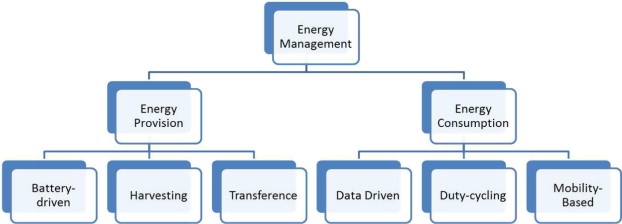
\includegraphics[width=0.95\textwidth]{energy-tax2.png}
 \end{center}
 \caption{The taxonomy of energy management schemes based on the source and the sink of the energy. (Source:~\protect\cite{khan2015})}
  \label{fig:energy-tax2}
\end{figure}
% 
%
%
While authors provided a classification of the energy management schemes in the paper, 
they also provided some statistical data related to these schemes. 
The survey that is given in the paper related to the energy transfer schemes is very unique and valuable information. 
Table~\ref{tab:etrans} summarizes these energy transfer schemes and their properties.

\renewcommand{\arraystretch}{2}%
\begin{table}[H]
\begin{center}
\caption{Current (as of 2018) energy transfer modes that can be used for WSNs. (Source:~\protect\cite{khan2015})}
\label{tab:etrans}
\begin{adjustbox}{max width=\textwidth}
\begin{tabular}{| l || l | l | l | l |} 
\hline
\rowcolor{lightgray}
\textbf{Technology} & \textbf{Efficiency (\%)} & \textbf{Range} & \textbf{Coverage} & \textbf{Remarks}\tabularnewline
\hline \hline
\cellcolor{lightgray} Wired                  & 90–95 & As desired & Limited to wires deployment & Static deployment, cost                     \tabularnewline \hline
\cellcolor{lightgray} Microwave beam         & 30–80 & >2 km      & Narrow beam                 & Potential hazards, line of sight required   \tabularnewline \hline
\cellcolor{lightgray} Magnetic Resonance     & 45–90 & 1–2 m      & Omnidirectional            & Limited range                               \tabularnewline \hline
\cellcolor{lightgray} Reflected Solar Energy & >90   & >1 km      & Narrow or wide beam         & Daytime only, line of sight required        \tabularnewline \hline
\cellcolor{lightgray} RF Energy              & 70    & 12–14 m    & Omnidirectional            & Limited range                               \tabularnewline \hline
\cellcolor{lightgray} LASER beam             & 10–18 & 1 km       & Narrow beam                 & Potential hazards, line of sight required   \tabularnewline \hline
\end{tabular}
%\\[1.0] %You can adjust how far below the table the text should appear
\end{adjustbox}
\end{center}
\end{table}
\renewcommand{\arraystretch}{1}%
% 






The paper~\cite{shaikh2016} provides a comprehensive survey of the energy harvesting technologies specific to WSNs. Classification of the harvesting technologies is
provided in the paper and also recent developments are discussed related to these technologies. Figure~\ref{fig:energy-tax4} shows the taxonomy of the harvesting
technologies that is given in the paper. Different from others, this paper considers two different harvesting sources. 
Namely ambient environment and external sources are listed as two possible harvesting source classes. Authors also provided tabular data related to various
popular sensor nodes and presented statistical data related to the properties and capacities of those energy harvesting sources.
% 
%
%
\begin{figure}[!htbp]
 \begin{center}
  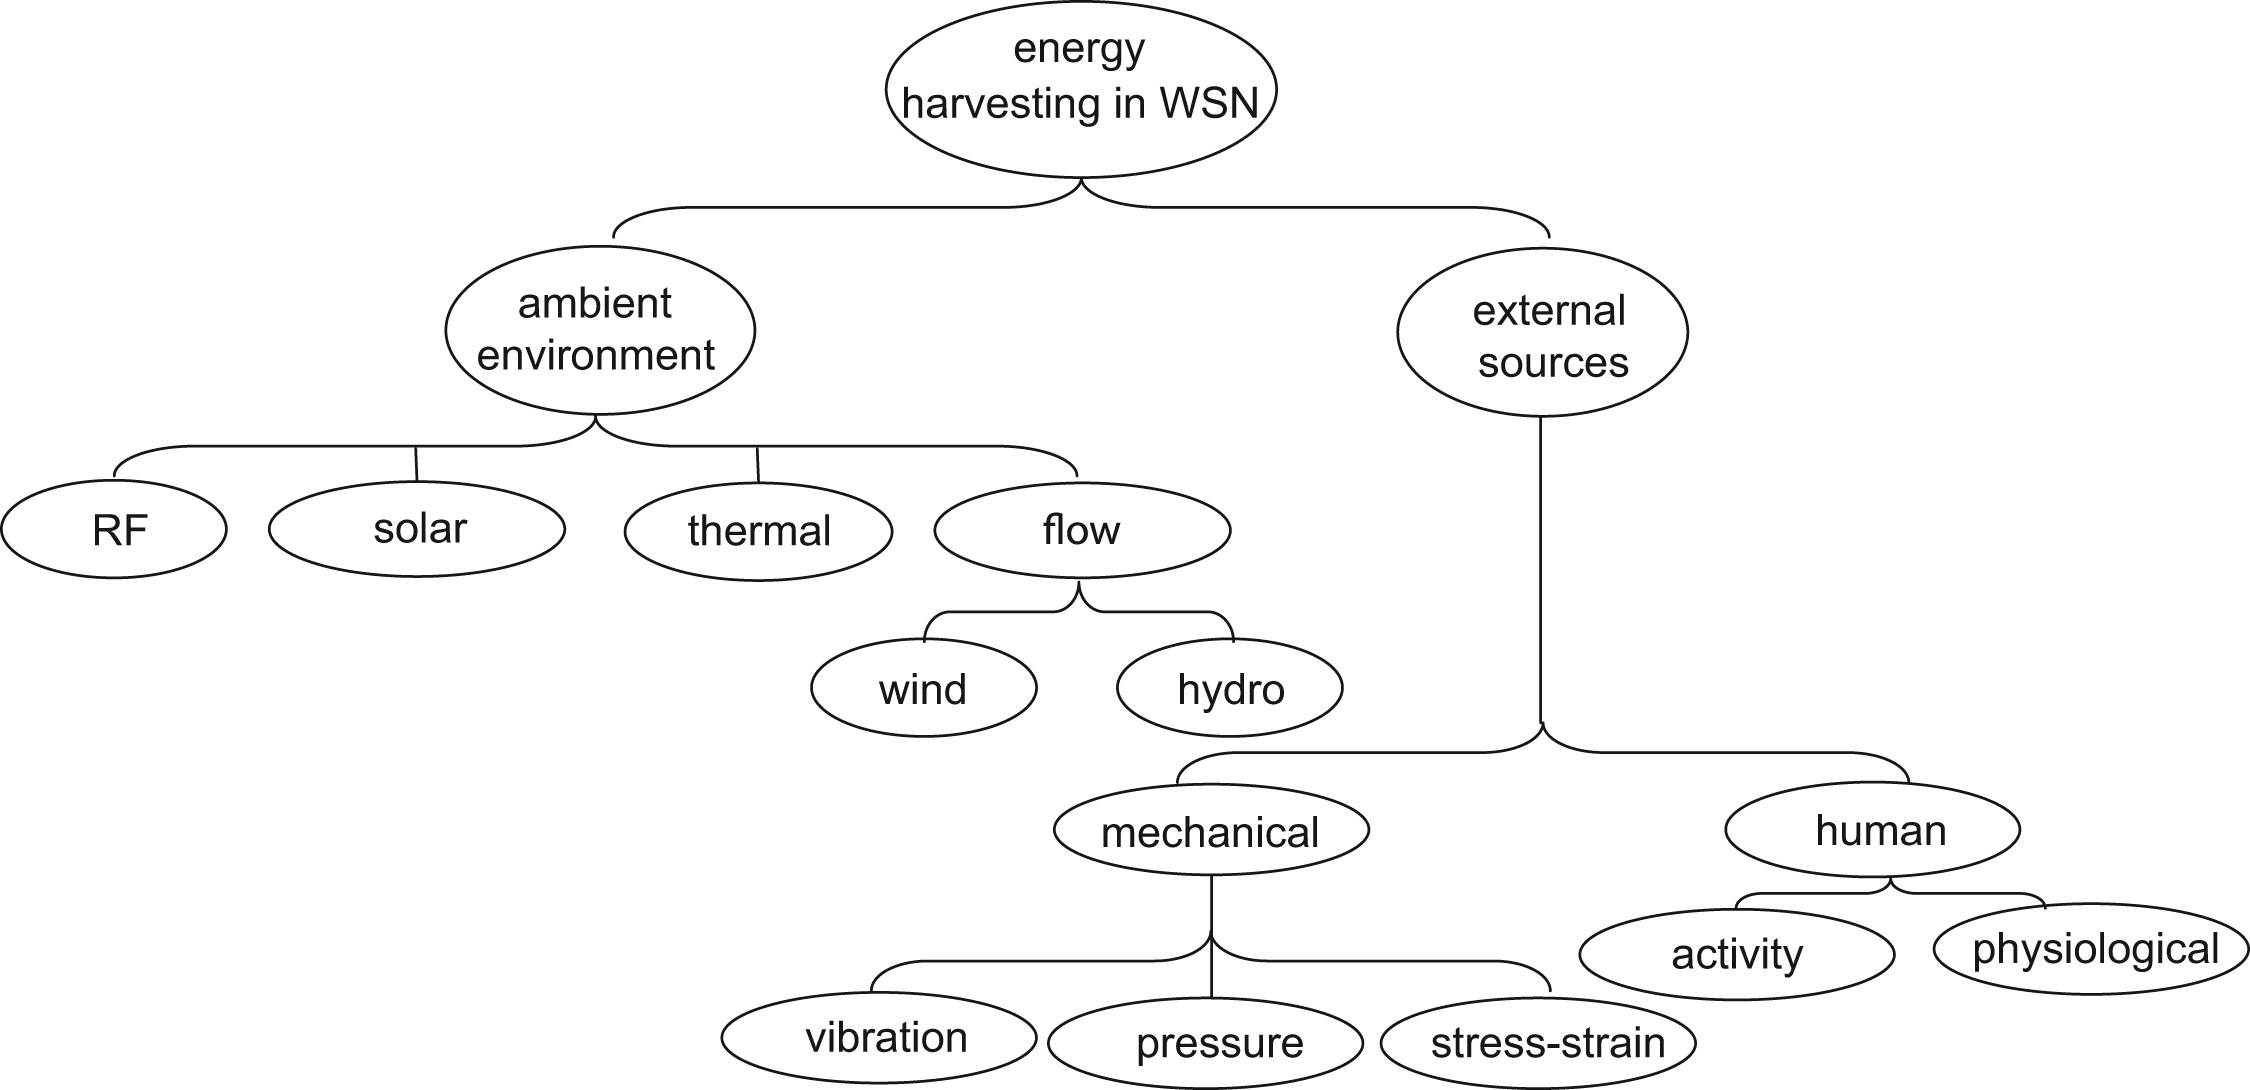
\includegraphics[width=0.95\textwidth]{energy-tax4.png}
 \end{center}
 \caption{Classification of the energy harvesting technologies that can be used in WSNs. (Source:~\protect\cite{shaikh2016})}
  \label{fig:energy-tax4}
\end{figure}
% 
%
%



In~\cite{akhtar2015}, the topic was energy replenishment from renewable and traditional energy resources. 
Authors presented a survey on the renewable energy sources and their characteristics. They also discussed
applications of such technologies in WSNs. For the traditional energy resources, the paper describes recharging
technologies for battery-operated WSNs.
The paper presents a taxonomy for the various energy resources that can be used in WSNs. 
Figure~\ref{fig:energy-tax3} gives the taxonomy authors provided. The paper looks the issue of energy problem in WSNs, from the point of sustainability
and provides taxonomy of energy resources that can be used in WSNs. Authors also provided discussion on the characteristics of each technology 
and commented on future research directions.
% 
%
%
\begin{figure}[!htbp]
 \begin{center}
  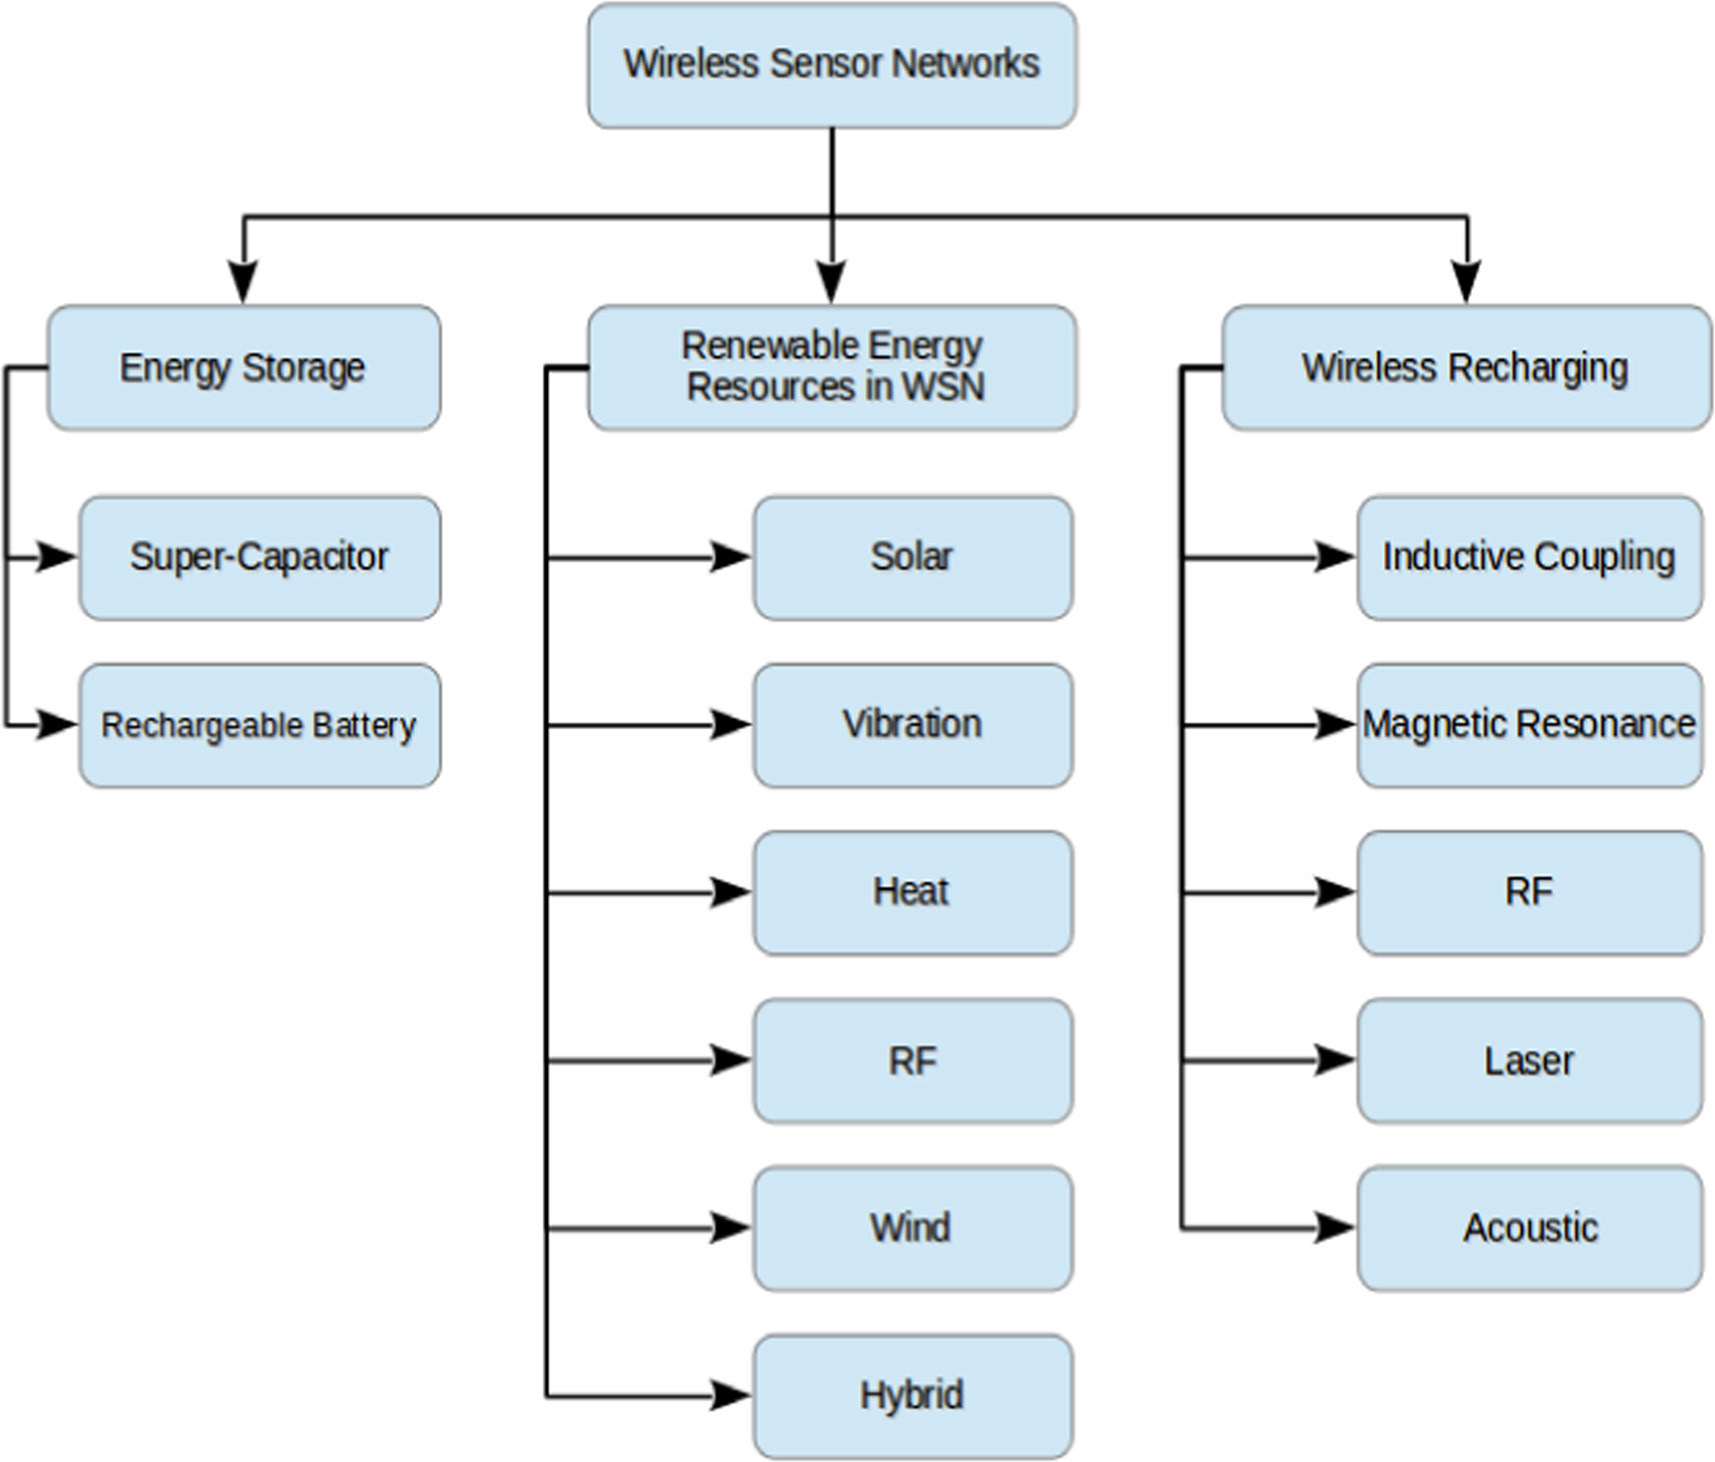
\includegraphics[width=0.95\textwidth]{energy-tax3.png}
 \end{center}
 \caption{Types of energy resources that can be used in WSNs. (Source:~\protect\cite{akhtar2015})}
  \label{fig:energy-tax3}
\end{figure}
% 
%
%



\newpage
The optimization techniques proposed in this thesis fall into two classes according to Figure~\ref{fig:energy-opt-techs}. 
The first one is directional antenna design which is in the class of "radio optimization".
The second optimization technique, namely energy-aware routing protocol, falls into "energy-efficient routing" class. 
An alternative classification of these energy optimization techniques
can be given by considering the layers of the Network Software that are used almost in every device that communicates. 
The network software is designed according to the ISO-OSI model consisting of 7 layers, which can be seen in Figure~\ref{fig:osimodel}. 
While the OSI model remained as 
theoretical reference model, in practice today TCP/IP model is used in communication. The relationship between OSI and TCP/IP model is shown in Figure~\ref{fig:osi-tcp}.
According to OSI layers, routing (path finding) is a function of the Network Layer (Layer 3), while the antennas are devices used in the Physical Layer (Layer 1).
%
%
%
\begin{figure}[!tbp]
  \begin{subfigure}[b]{0.48\textwidth}
    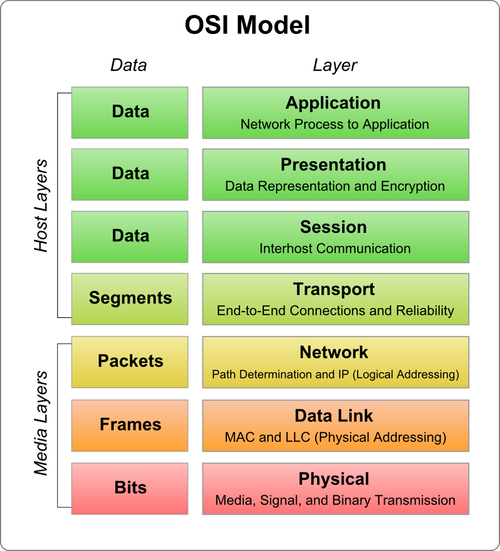
\includegraphics[width=\textwidth]{osimodel.png}
    \caption{The ISO-OSI model and the layers of the Network Software. (Source:~\protect\cite{osimodel})}
    \label{fig:osimodel}
  \end{subfigure}
  \hfill
  \begin{subfigure}[b]{0.48\textwidth}
    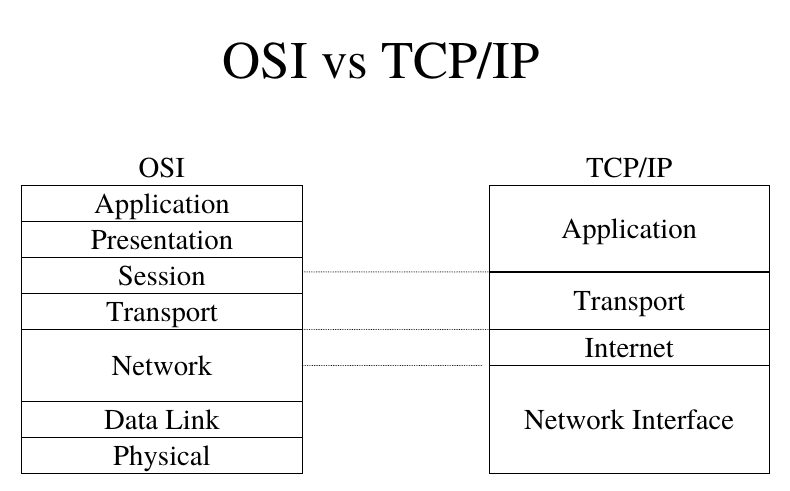
\includegraphics[width=\textwidth]{osi-tcp.png}
    \caption{OSI vs TCP models. (Source:~\protect\cite{bathula2007})}
    \label{fig:osi-tcp}
  \end{subfigure}
  \caption{OSI and TCP layers.}
\end{figure}

% 
% % 
% %
% %
% \begin{figure}[!htbp]
%  \begin{center}
%   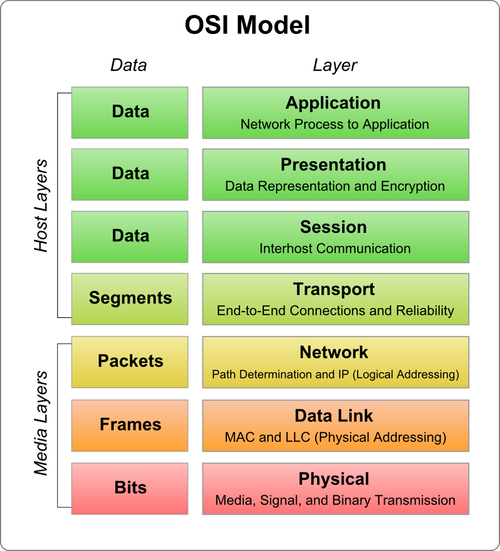
\includegraphics[width=0.6\textwidth]{osimodel.png}
%  \end{center}
%  \caption{The ISO-OSI model and the layers of the Network Software. (Source:~\protect\cite{osimodel})}
%   \label{fig:osimodel}
% \end{figure}
% % 
% %
% %
% 
% % 
% %
% %
% \begin{figure}[!htbp]
%  \begin{center}
%   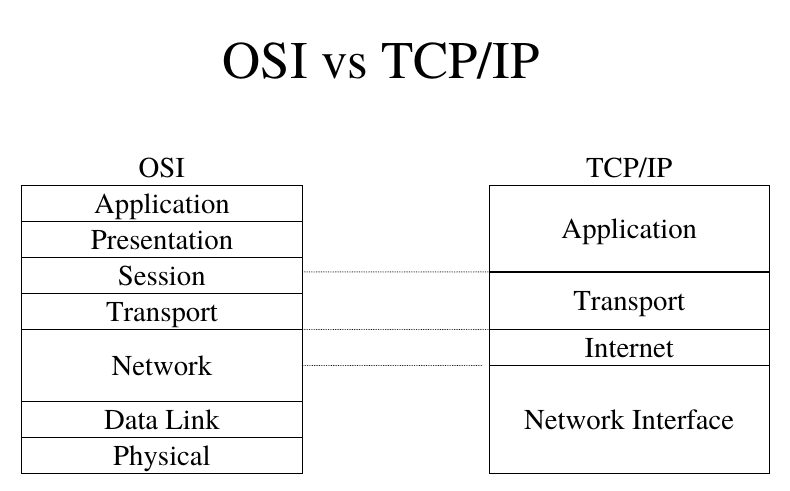
\includegraphics[width=0.7\textwidth]{osi-tcp.png}
%  \end{center}
%  \caption{OSI vs TCP models. (Source:~\protect\cite{bathula2007})}
%   \label{fig:osi-tcp}
% \end{figure}
% % 
% %
% %


%%%%%%%%%%%%%%%%%%%%%%%%%%%%%%%%%%%%%%%%%%%%%%%%%%%%%%%%%%%%%%%%%%%%%%%%%%%%%%%%%%%%%%%%%%%%%%%%%%%%%%%%%%%%%%%%%%%%%%%%%%%%%
% 
% \chapter{Related Work and Proposed Solutions}\label{crelworkandsoln}
% %
% In this thesis, two methods are studied for the energy usage optimization. While the main goal is to maximize the network lifetime, the two solutions offered 
% for the energy problem can be associated with the optimizations at different levels. At the SW level thesis will present energy aware routing protocol and 
% will discuss enhancements for using the routing method with directional antennas. At the HW level, simple patch-array antenna design will be presented and
% energy savings that come from the directional nature of the antenna, along with the issues that are related to the directionality will be explained in the thesis.
% In Section~\ref{srouting}, the energy aware routing protocol topic will be discussed. 
% The survey of the studies related to the routing algorithms will be presented in Section~\ref{ssroutingwork}. 
% After that, design description and implementation details about the LaGOON protocol and performance evaluations will be given
% in Section~\ref{clagoon} and in Section~\ref{sperf} respectively.
% 
% 
% Section~\ref{cdantenna} will discuss the design and implementation of the directional antenna proposed in this thesis. Following that in sub sections,
% introduction to antenna characteristics, literature survey, and an assessment on the designed directional antenna will be presented.
% In Section~\ref{santbas} basic information, related to the antennas will be given, with the emphasis being on the differences between directional and omnidirectional antennas.
% Section~\ref{santresearch} will be on the literature survey related antennas, mostly focused on the use of directional antennas in WSNs. Finally, Section~\ref{sspropdant} will
% discuss the characteristics and the performance properties of the proposed microstrip patch antenna array. 


\newpage
%%%%%%%%%%%%%%%%%%%%%%%%%%%%%%%%%%%%%%%%%%%%%%%%%%%%%%%%%%%%%%%%%%%%%%%%%%%%%%%%%%%%%%%%%%%%%%%%%%%%%%%%%%%%%%%%%%%%%%%%%%%%%
\chapter{Energy Aware Routing}\label{cwsnrouting}
\vspace{-1.7cm}

Routing is one of the most important functions that can be applied to the SW part of the system. The goal in routing is basically
finding a path for packets from source to destination, which generally known as "forwarding" or "routing". Routing is called
"path finding" in some sources.
Many design factors and constraints should be considered together for the design and implementation of the routing protocol.
For example, the effect of the topology of the nodes, which is mainly a HW property of the system, can be effective on routing too. 
The energy efficiency is one of the most important factors a routing should handle while trying to "route" packets.
In multi-hop networks, the delivery of 
the message should take the least "costly" path from source to destination. The "cost" can be associated with many of the QoS
requirements. "Least energy usage" is one of the most important QoS attributes. 
In any network where energy is very much limited, like WSNs, "minimum energy usage" for the routing is vital, as the communication consumes 
the most power.
In this sense, "energy-aware" or "energy-effective" routing tries to minimize the overall energy usage of the transmissions. 
The goal is to prolong the network lifetime while forwarding packets to their destinations so that the maintenance cost will decrease and the autonomy of the WSN will increase.
The first solution proposed in this thesis is a simple energy aware routing protocol, which can be 
regarded as SW optimization method. This method is studied for WNSNs (Wireless Nano Sensor Networks) and for WSNs.
The methodology that is applied for the research on the routing involved, firstly, a literature survey both in breadth and depth for getting an overview
of the research activities and discovering the gaps in the field respectively. After that the idea of the simple energy aware routing is implemented by using
a suitable simulator for performance assessment. 
In the following sections short literature review is presented related to the topic and then the general overview of the proposed
routing algorithm is given. Finally, simulations and results are discussed in detail for each solution.


\newpage
\section{Routing Research in WNSN}\label{sroutingWNSN}


Routing has a special stature in the WNSNs. Not only WNSNs are new technologies, but also they are fundamentally different technologies.
Although there is no standard routing protocol for WNSNs yet, several promising studies are published.
Unfortunately, current network protocols can not be applied to nano communication. They are too complex for nano sensors and the energy constraints of
nanosensors can not sustain such protocols. Due to the nanoscale dimensions of the sensor nodes and the size of their antennas, 
THz frequency is the only band that the communication can be done.
As a result new protocols, new modulation techniques, and new signal encoding methods are necessary for THz frequency communications. 
The only work toward practical standardization is the framework IEEE 1906.1~\cite{ieee-1906}, which contains recommendations.

However, there are several studies focused on different aspects of the nano communication, like physical layer, THz antenna technology, routing, 
and energy harvesting.
Several aspects can be considered in the design of a routing protocol such as the nano-network topology, multi phase settings, mobility, 2D-3D.
But, according to current nanotechnology studies such as~\cite{akyildiz2010-2, pierobon2014}, the most important and most limiting factor is the energy.
In that sense, the special case of routing protocol design for the WNSNs can be seen as energy optimization problem with various constraints.
Routing protocols in nanonetworks can be classified into two main groups. Mainly, unicast protocols like simple flooding and multicast protocols like random point-to-point protocol. 
While in the flooding simply every node forwards the received message, in point-to-point group protocols, 
forwarding is done to a specific node based on certain criteria.

Studies like in the following paragraphs, tried to develop routing frameworks focusing on different layers of the network. However, it can be seen 
that comprehensive routing framework not only requires cross-layer design, but also collaborative involvement of various engineering departments.
The ideal optimized routing requires synergy among various parts of the sensor node architecture such as, antenna, signal encoding method, duty-cycling mechanism, 
routing software, customized packet format, addressing scheme, and power unit controller. On the other hand, such efforts are the first steps towards standardization.
In this sense, the performance comparison among these methods not only can be difficult, but also can not fully explain the isolated algorithm performance.
However, several promising works can be listed, like the ones in~\cite{zhou2012, yu2015, liaskos2015, liaskos2016, afsana2018}. 
The studies in~\cite{tairin2017, abuali2018}, provide survey and overview on the routing research 
related to the nanonetworks.


%
% HERE Table with characteristic of routing
% Topology 1D 2D 3D
% Type peer-to-peer, flooding, 
% Metrics delay, throughput, etc..
% Energy?
% Criteria 
% Application area

%

Authors in~\cite{zhou2012}, focused on the physical layer part for their routing protocol. They proposed Physical Network Coding based
"pair-to-pair" routing framework by extending the geographical greedy routing algorithm. The packets are divided into two parts 
and transmitted in pairs along the pipelined multi-hop route, with the idea of gathering weak nodes into groups where integrated routing can be
achieved for energy efficiency. The paper extends the idea of GPSR (Greedy Perimeter Stateless Routing) in~\cite{karp2000}. While the GPSR 
is point-to-point routing algorithm, authors extend it to be a pair-to-pair routing in their work, calling it "Buddy Unicast" routing.
Although the Buddy routing is not energy efficient, its performance in throughput is very high.


In~\cite{yu2015}, a channel-aware routing protocol is proposed. Authors considered the special attributes of the THz band communication.
The forwarding is optimized by considering two cost factors, namely avoiding long-distance region in which the signal may suffer the 
path loss and avoiding the short-distance region in which the number of hops may be increased unnecessarily. For the simulations 1D "string"
network topology is considered. The paper considered metrics like end-to-end performance, end-to-end capacity and
end-to-end delay. For the parametric simulations, authors used different node densities and different water percentages representing 
various human body tissue characteristics, as the targeted application was in-body health monitoring system.
The proposed routing algorithm achieved high channel capacity and exhibited low hop count reducing transmission delays.


In~\cite{liaskos2015}, coordinate-based addressing scheme, CORONA, is proposed for nanonodes placed uniformly in a rectangular 2D topology.
The proposed routing protocol tries to minimize the hop count of the packet transmission by placing anchor nodes 
at the vertices of the grid and using the coordinate based addressing scheme as it can be seen in Figure~\ref{fig:anchor}.
Through simulations, the routing protocol is assessed by considering the packet retransmission
rate, successful packet reception rate, and packet loss rate. According to the simulations done in the paper, 
CORONA showed low packet retransmissions and low energy consumption compared to the flood routing. However, the paper stated that 
global packet reception rate is very low for CORONA.
Although the paper does not present an energy efficiency measure, the energy efficiency is associated with the metrics that are used 
in the simulations, such as global packet send (packets per nano second), receive and interference rate .
% 
%
%
\begin{figure}[!htbp]
 \begin{center}
  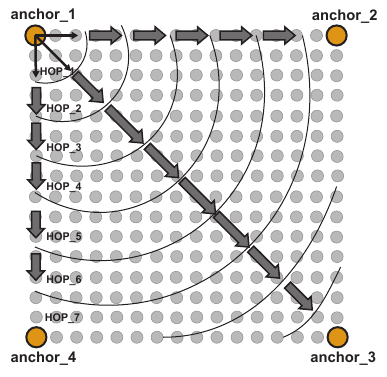
\includegraphics[width=0.4\textwidth]{anchor.png}
 \end{center}
 \caption{The anchor nodes based coordinate system. (Source:~\protect\cite{liaskos2015})}
  \label{fig:anchor}
\end{figure}
% 
%
%
\vspace{-0.5cm}

In~\cite{liaskos2016}, authors proposed peer-to-peer type routing protocol. For the simulations, 2D uniform grid and 2D uniform random
topologies are assumed, in which identical nanonodes are deployed. The assumption for the nano communication was 100GHz frequency with standard atmospheric conditions.
This condition is assumed for providing the minimum effect for the path loss due to molecular absorption and high data rate.
Packet collisions and redundant retransmissions, being the two metrics that are considered in the paper, 
are optimized in the proposed protocol. During the setup phase, nodes are classified based on the packet reception 
statistics they have logged. The routing scheme exploits this classification.

The paper~\cite{afsana2018} proposes an energy conserving protocol based on the hybrid clustering of the nanonodes and centralized scheduling.
The proposed method, Nano Cluster Composition Algorithm (NCCA), offers a model which designed for channel behavior, by considering 
aggregated impact of molecular absorption, spreading loss, and shadowing. The energy model of NCCA considers harvesting in addition to the consumption.


In~\cite{tairin2017}, authors pointed out the lack of research related to the protocols in higher network layers for the WNSNs. 
They also added that most research is focused on the lower network layers, especially on the MAC layer and Physical layer. 
After benchmarking classical WSN protocols like AODV (Adhoc On-demand Distance Vector)~\cite{RFC3561, jhaveri2015, hofner2012}, DSDV (Destination Sequenced Distance Vector)~\cite{perkins1994}, 
and DSR (Dynamic Source Routing)~\cite{johnson2001}, on WNSN, authors find out that AODV performs better in WNSNs. Their performance metrics criteria include packet delivery ratio, 
throughput (Kbps), average delay, packet drop rate, and energy consumption. As a parameter, the paper proposes a varying number of nanonodes (50, 100, 150, 200) for 
simulating networks with varying densities, from sparse to dense.
The paper based on this benchmarks, proposed a modified version of AODV as "Hierarchical AODV" routing protocol. The protocol which is customized for 
WNSNs performed better than all the others.


The paper~\cite{abuali2018}, provides benchmarks for the current nano communication routing protocols.
In the benchmarks, three routing protocols were considered. Namely, controlled flooding, coordinate routing (CORONA~\cite{liaskos2015}),
and Hierarchical AODV (\cite{tairin2017}). The performance metrics were focused on the number of successfully delivered packets, delay, and energy consumption. 
Authors used parameters as number of nanonodes (50-250 nodes, sparse to dense network spectrum) and their transmission range (1mm, 10mm, 15mm, 20mm). 
CORONA and controlled flooding are found to be worst in delay and energy
consumption for increasing number of nodes and transmission ranges. While the Hierarchical AODV protocol is found to have the best energy consumption, 
it presented higher complexity and lower throughput. 






\newpage
\section{Routing Research in WSN}\label{sroutingWSN}


Compared to the WNSNs, in the field of WSNs, routing is studied in much more depth and breadth. Nanosensor nodes are very new technology compared
to the classical sensor nodes. Routing by itself studied since the beginning of the computer networks.
It is interesting to take a look at one of the early papers on routing in mobile networks like the paper from 1996 by Ramanathan~\cite{ramanathan1996}.
Several papers can be regarded as some of the first efforts to consider energy as metric in routing like~\cite{singh1998, rodoplu1999, stoj2000}, and~\cite{stoj2001}.
With the LEACH (Low Energy Adaptive Clustering Hierarchy) paper (\cite{heinzelman2000}) energy based routing and clustering gained momentum and LEACH protocol
became standard benchmarking algorithm for most of the energy based protocols. The comprehensive survey on the historical development of the LEACH-based protocols
can be found in~\cite{singh2017}.
There are many ways to classify existing routing protocols.  
Especially the case had been studied extensively for the wireless sensor networks in~\cite{kamal2004, bazzi2015, pantazis2013, sarkar2016}. 
In the following paragraphs, different works are presented related to the classification of the routing protocols and related to the 
issues in designing routing protocols.



The paper~\cite{kamal2004} presents a comprehensive survey on the routing techniques in WSNs. Authors provided a framework for their classification by
describing the architecture of the sensors and listing challenges in routing along with the design issues related to the WSNs. In Figure~\ref{fig:kamal-tax} the proposed
classification of the routing protocols can be seen. 
The paper bases the classification presented, on the network structure (external) of the WSN and on the behavior of the routing protocol (internal) in the nodes.
% 
%
%
\begin{figure}[!htbp]
 \begin{center}
  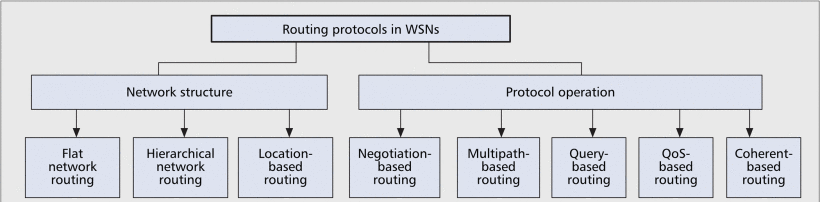
\includegraphics[width=\textwidth]{kamal-tax.png}
 \end{center}
 \caption{Taxonomy of routing protocols in WSNs. (Source:~\protect\cite{kamal2004})}
  \label{fig:kamal-tax}
\end{figure}
% 
%
%

\newpage


The paper~\cite{farooq2011} presents a survey on the operating systems for WSNs and lists several characteristics of the WSNs (nodes), 
like size, scarce resources being important factors in the design of software and hardware of the WSNs. 
Authors also present optimizing sensors' lifetime as a fundamental objective and they comment on the necessity of the new design paradigm. 
The paper is valuable in the sense of analyzing the sensor node system in holistic way by considering both SW and HW.
In doing so, the paper provides the reader a broader panorama for viewing the place and the interaction of the routing in the sensor node system architecture.

In~\cite{ndie2012}, authors focused on the constraint based routing protocols. They basically considered routing algorithms
considering limited power, low computing power, low storage,  and short-range radio communication. The paper claimed that while there are efforts
in designing constraint based routing protocols for WSNs, still there are no formal and standard solutions offered in this direction. Authors
proposed configuration management based routing protocol for WSNs.


According to~\cite{pantazis2013} the study~\cite{akyildiz2002-2} introduced the framework for the design issues related to the issues related to network layer stack,
while leaving out the classification of the routing protocols. In this work authors presented a framework for routing protocols by considering energy consumption models for nodes
and traffic patterns for their communication. Figure~\ref{fig:traffic} shows the traffic patterns in~\cite{pantazis2013} considered.
% 
%
%
\begin{figure}[!htbp]
 \begin{center}
  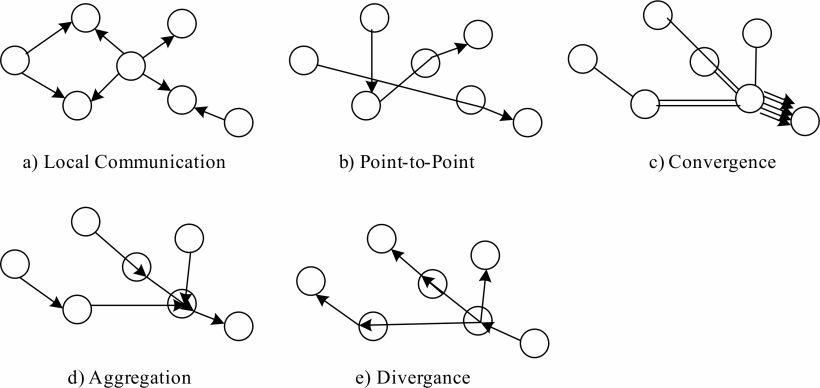
\includegraphics[width=\textwidth]{traffic.png}
 \end{center}
 \caption{Traffic patterns specific to WSNs. (Source:~\protect\cite{pantazis2013})}
  \label{fig:traffic}
\end{figure}
% 
%
%

In the energy consumption model, they consider energy cost for sensor state changes, processing, and communication. The paper lists
asymmetric, WSN specific traffic patterns due to the way the data are collected in WSNs. 
This is due to the fact that, generally sensor nodes send data to sink nodes and the sink node
very sporadically sends control messages to sensor nodes.
The classification paper proposes for the routing protocols can be seen in Figure~\ref{fig:tax-pantazis}.
% 
%
%
\begin{figure}[!htbp]
 \begin{center}
  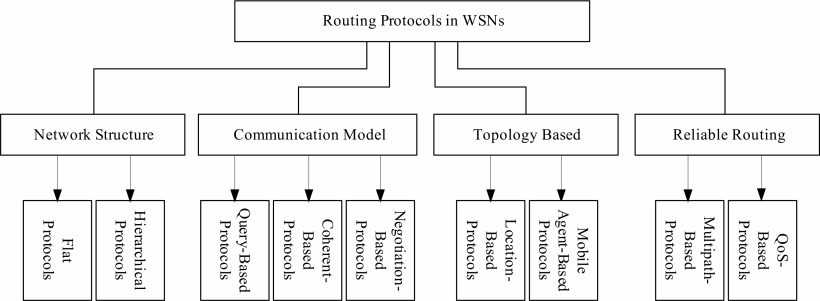
\includegraphics[width=0.95\textwidth]{tax-pantazis.png}
 \end{center}
 \caption{Classification of the routing protocols for WSNs. (Source:~\protect\cite{pantazis2013})}
  \label{fig:tax-pantazis}
\end{figure}
% 
%
%
\vspace{-0.7cm}
% 
%
%
\begin{figure}[!htbp]
 \begin{center}
  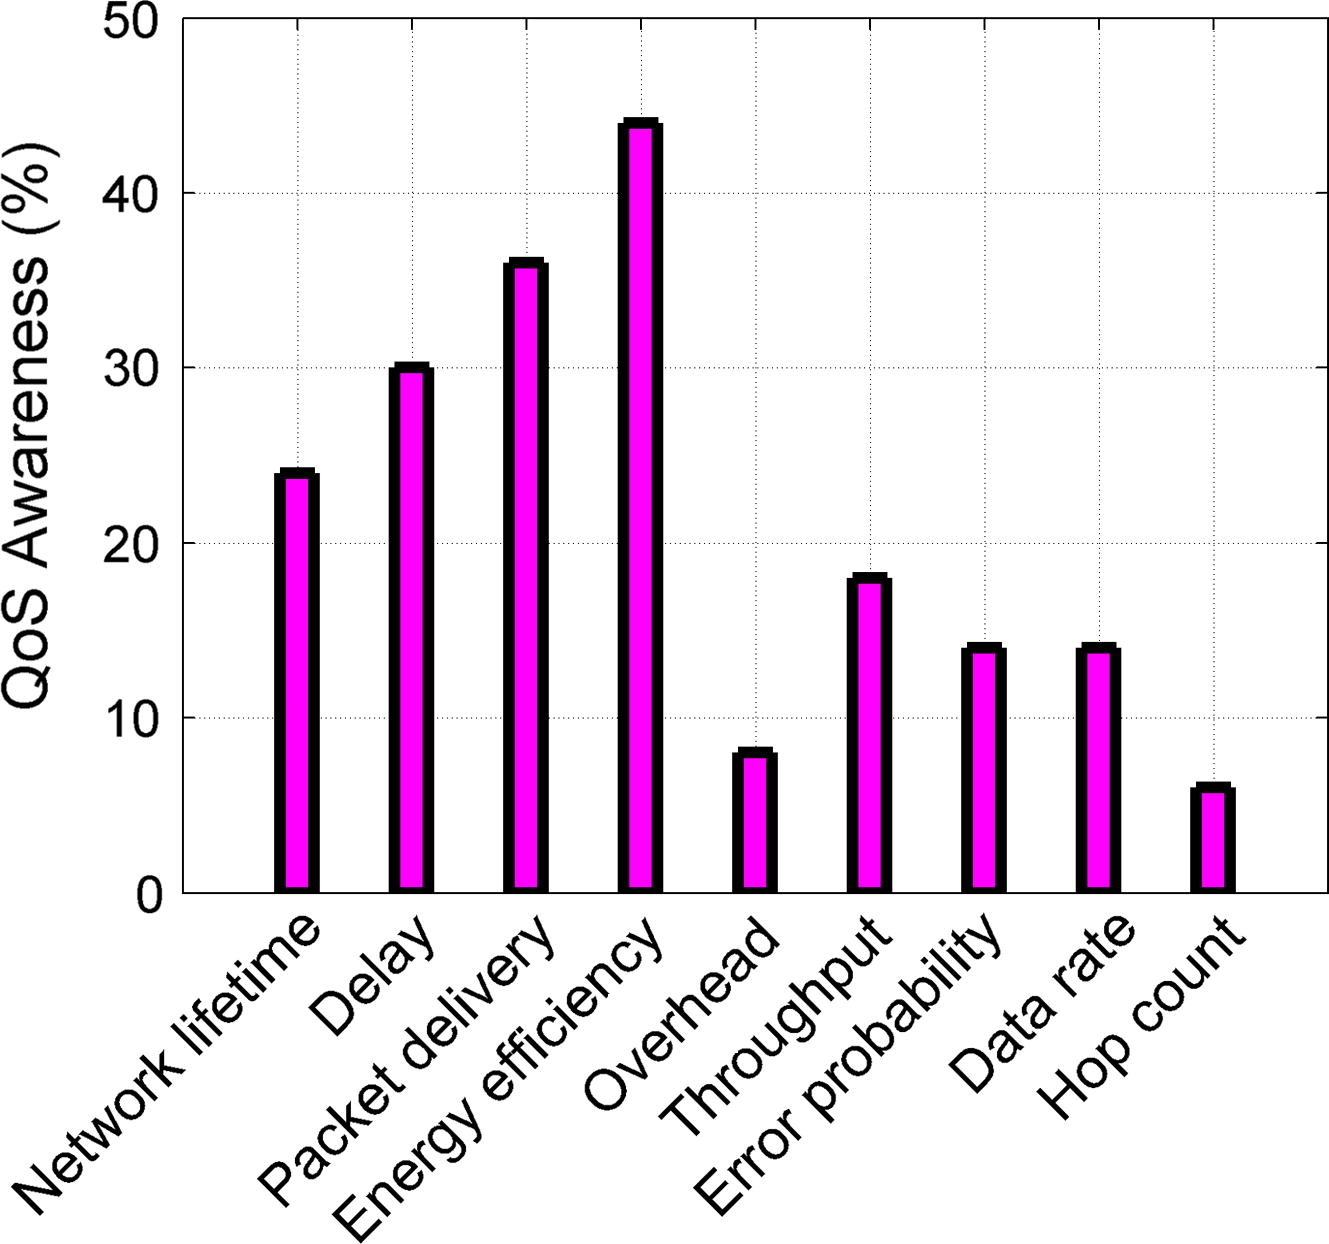
\includegraphics[width=0.5\textwidth]{routing-research.png}
 \end{center}
 \caption{The distribution of the research on QoS parameters. (Source:~\protect\cite{sarkar2016})}
  \label{fig:routing-research}
\end{figure}
% 
%
%
\vspace{-0.7cm}

The topic of the paper~\cite{sarkar2016} was "the research in routing" itself.
The paper, not only provides a valuable survey and classification of the routing algorithms for WSNs, but also provides statistical data
on the research situation of the routing algorithms. In Figure~\ref{fig:routing-research}, one such statistical data is given related 
to the percentages of the papers published for each QoS parameter. The top group is the "energy efficiency", consisting 44\% of the publications. 


In thesis~\cite{pitchai2015} the author proposed three energy efficient routing. In the first method, 
Game Theory used in clustering based routing protocol for energy savings in WSNs.
The second energy efficient method that was proposed involved Graph Theoretic Connected Dominating Set (CDS) concept.
Domination is an active research area of Graph Theory where various optimization problems are tackled. 
The roots of the concept go to N-Queens problem (\cite{bell2009}). In computer networks Dominating Set is used for
maintaining the hierarchical structure where nodes in the Dominating Set (DS) can communicate better.
A Connected Dominating Set (CDS~\cite{cds}) is a dominating
set in a computer network, which nodes are connected (reachable) to each other.
Based on these four attributes a network can be called CDS:
\vspace{-0.5cm}
\begin{itemize}
\setlength\itemsep{0em}
\item Connected, so that routing is possible.
\item Reasonably small for cost effectiveness.
\item Contains shortest paths for effective routing.
\item Consists of nodes with enough energy.
\end{itemize}
\vspace{-0.5cm}
In Figure~\ref{fig:cds} sample WSN is shown along with the DS and CDS. Better routing can be achieved with smaller DS. 
So constructing Minimum Connected Dominating Set (MCDS) in WSN is desirable.
% 
%
%
\begin{figure}[!htbp]
 \begin{center}
  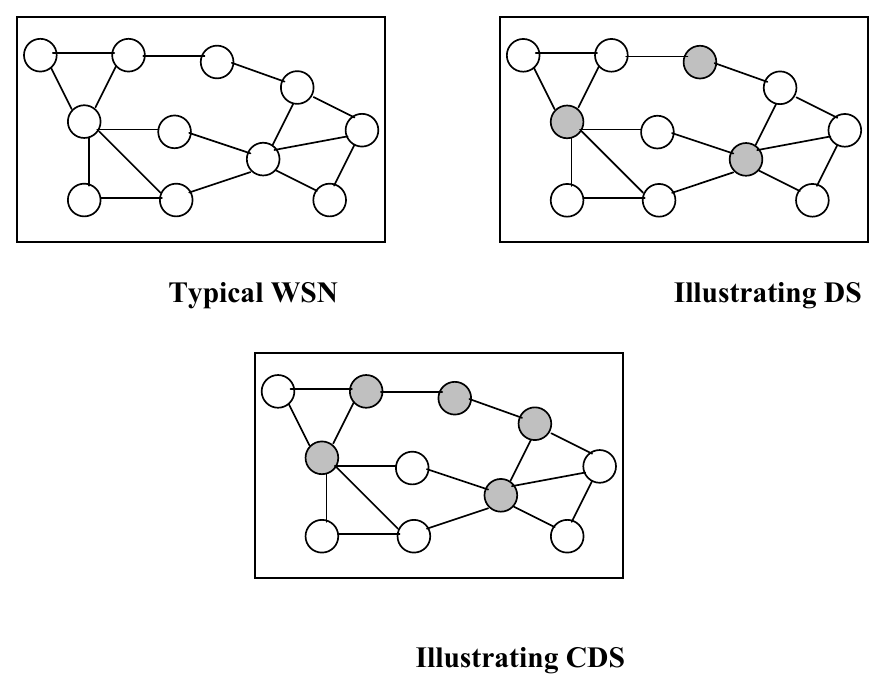
\includegraphics[width=0.80\textwidth]{cds.png}
 \end{center}
 \caption{Example WSN and its DS and CDS. (Source:~\protect\cite{pitchai2015})}
  \label{fig:cds}
\end{figure}
% 
%
%

\newpage
The third routing scheme proposed in the thesis was based on the bio-inspired swarm optimization. 
The energy aware clustering based routing protocol inspired by honey bee colony is proposed as
optimal routing with the minimum number of hops in communication.



The routing protocols mentioned in previous discussions like AODV and DSR are all
"single path" routing algorithms. That means the algorithms propose single path
information for forwarding packets. However, there are "multi-path" routing algorithms 
that can offer more than one routing paths. In~\cite{hurni2008} authors proposed such multi-path
routing algorithms as an optimization to energy constraint.
The paper claimed that multiple routes are useful because of the dynamic and unpredictable
nature of the ad hoc networks. Further authors stated that for WSNs multi-path routing focuses
on load-balancing or fault tolerance.
The paper listed the benefits of the multi path routing as:
\vspace{-0.5cm}
\begin{itemize}
\setlength\itemsep{0em}
\item \textbf{Load Balancing:} Congestion avoidance and improved performance.
\item \textbf{Fault Tolerance:} Redundant information routed to the destination node in multi paths increase fault-tolerance.
\item \textbf{Bandwidth Aggregation:} Data to the destination node, can be split into multiple streams and each stream can be routed 
in multi paths simultaneously.
\item \textbf{Reduced Delay:} In WSNs in case of node failure alternative routes should be found. This causes delays in transmission.
However multi-path routing can reduce these delays since there can always be alternative routings.
\end{itemize}
\vspace{-0.5cm}
Firstly the paper describes several multi-path routing algorithms like Ad hoc On
Demand Distance Vector Multi-path routing protocol (AODVM)~\cite{ye2003}, Ad hoc On Demand Multi-path Distance
Vector protocol (AOMDV)~\cite{marina2001} (extension of AODV for discovering paths that are node-disjoint or link-disjoint),
and Split Multi-path Routing (SMR)~\cite{lee2001}. Then the paper describes the proposed energy-efficient multi-path routing based on AOMDV.
The design of the proposed routing algorithm involved the integration of the MAC protocol with periodic wake-up and multi-path routing protocol.
While the sleep/wake-ups cycling increases the network lifetime, it also provides load-balancing. The paper reports 10-15\% performance
increase in lifetime and end-to-end communication delay.




\pagebreak

In~\cite{bazzi2015}, authors considered the routing from the designer's point of view, listing 17 factors that they deemed important in the design of a routing algorithm. 
In Table~\ref{tab:bazzi} below, these factors and the situations that they are effective are summarized.


\renewcommand{\arraystretch}{1.25}%
\begin{table}[H]
\begin{center}
\caption{Factors and the situations that should be considered in designing routing algorithm for WSNs. (Source:~\protect\cite{bazzi2015})}
\label{tab:bazzi}
\begin{adjustbox}{max width=\textwidth}
\begin{tabular}{| l | l |} 
\hline
\rowcolor{lightgray}
\textbf{Factor} & \textbf{Situation} \tabularnewline
\hline \hline
Energy Consumption     &  {\parbox[t]{10cm}{The life of a node depends on its battery which is limited and small considering the node's size.}} \tabularnewline \hline
Scalability            &  {\parbox[t]{10cm}{The Routing protocol used must be able to handle large number of nodes.}} \tabularnewline \hline
Connectivity           &  {\parbox[t]{10cm}{Nodes must stay in connection even after some node failure.}} \tabularnewline \hline
Network costs          &  {\parbox[t]{10cm}{The cost of a node affects the cost of the whole network.}} \tabularnewline \hline
Data aggregation       &  {\parbox[t]{10cm}{Multiple nodes may generate redundant data causing an unnecessary traffic. Similar data can be aggregated, combined, to reduce the transmission.}} \tabularnewline \hline
Quality of service     &  {\parbox[t]{10cm}{The routing protocol must deal with the demands needed for an application.}} \tabularnewline \hline
Fault tolerance        &  {\parbox[t]{10cm}{The routing protocol must be able to reroute a packet if any node fails, in order to reach the sink.}} \tabularnewline \hline
Mobility               &  {\parbox[t]{10cm}{The routing protocol should handle topology changes and should consider the energy a node uses for relocation.}} \tabularnewline \hline
Node deployment        &  {\parbox[t]{10cm}{The routing protocol should consider the deployment of nodes which can be random.}} \tabularnewline \hline
Environmental conditions &  {\parbox[t]{10cm}{Sensor nodes must be able to overcome any environmental condition.}} \tabularnewline \hline
Hardware constrains  &  {\parbox[t]{10cm}{Sensor nodes can vary in size, in architecture, in types of power units they have.}} \tabularnewline \hline
Transmission media  &  {\parbox[t]{10cm}{Wireless links can be formed by infrared, radio, or even optical media.}} \tabularnewline \hline
Network topology  &  {\parbox[t]{10cm}{For high number of nodes a good topology maintenance plan must be followed.}} \tabularnewline \hline
Deployment phase &  {\parbox[t]{10cm}{Sensors can be manually deployed, one by one, or randomly deployed, by a plane or missile.}} \tabularnewline \hline
Post-deployment &  {\parbox[t]{10cm}{Topology can change due to relocating nodes in case of environmental changes, malfunction of a node, or even death of a node (no energy).}} \tabularnewline \hline
Redeployment  &  {\parbox[t]{10cm}{To keep this sensor network functioning, additional nodes may be added to replace the lost nodes.}} \tabularnewline \hline
Security   &  {\parbox[t]{10cm}{Data transmitted must be secured from any external attacks or unauthorized access.}} \tabularnewline \hline
\end{tabular}
%\\[1.0] %You can adjust how far below the table the text should appear
\end{adjustbox}
\end{center}
\end{table}
\renewcommand{\arraystretch}{1}%
% 





\pagebreak




In~\cite{benaddy2017}, authors pointed out the lack of consideration of the energy optimization in the design of a reliable multi-path routing algorithms.
In their approach to the reliable multi-path routing, they proposed a conceptual model in which constraints like distance and energy consumption are included. 
The algorithm proposed in the paper 
consists of two phases. The first one is the "construction" phase in which special packets called "weight setup packets" are utilized. In the second part, 
which is called "data transmission" phase, the actual transmission begins. For this conceptual framework, authors are planning to carry out simulations
as a future work.





%%%%%%%%%%%%%%%%%%%%%%%%%%%%%%%%%%%%%%%%%%%%%%%%%%%%%%%%%%%%%%%%%%%%%%%%%%%%%%%%%%%%%%%%%%%%%%%%%%%%%%%%%%%%%%%%%%%%%%%%%%%%%
\newpage
\chapter{Proposed LaGOON Routing Protocol}\label{clagoon}

Considering the limitations of the WNSNs and WSNs along with the high energy cost of communication, a simple energy-efficient 
routing protocol, "LaGOON" (Last GOOd Neighbor), is proposed and benchmarked in this thesis.
The proposed routing algorithm is called "LaGOON" (Last GOOd Neighbor) as it applies "backward learning" and remembers the "last good neighbor" in making routing decisions. 
As the nanodevices have a simple hardware, rather restricted software is needed. The layered structure for the TCP protocol stack 
was proposed to overcome complexities of big software systems. However, for the nanodevices, software should be rather simple and efficient.
The routing protocol should not introduce unnecessary communication overhead and has to be energy efficient. 
In this context two main principles have guided the design of the LaGOON, were to keep the least 
communication overhead
and to use the simplest data structures that are necessary for the routing functionality. 
The basic idea was to make use of the information in the arriving packets as much as possible, 
with the assumption of symmetric communication. 
The adaptive "Backward-Learning" paradigm utilizes the "path length" (from TTL) information and the "source" of the path for future transmissions.
Moreover, the proposed method does not assume any specific topology. 
Since it involves an evolving distributed scheme, the proposed method can handle both mobile and static configurations in communication systems.
Here the method offers optimization at the global level (covering all the network).
Energy efficient or aware routing protocol is essential for optimizing the overall energy usage of the sensor network and increasing the lifetime of sensors.
Mostly, the implementation of the proposed energy-aware routing protocol involves static topologies. 
On the other hand, mobility can be handled by the proposed method 
with some delays and overheads in the communication.

In the case of WNSNs, it offers less energy consumption compared to flooding and random routing protocols. 
It is simulated by using "ns-3\footnote{\url{https://www.nsnam.org}}", which is a discrete-event network simulator for Internet systems, 
and "Nano-Sim\footnote{\url{https://telematics.poliba.it/index.php?option=com_content&view=article&id=30&Itemid=204&lang=en}}" library of the ns-3, which is developed for
nanonetworks~\cite{piroNS32013, piroPA2013}.
In conducting this study, WNSNs have been chosen on the basis of their very limited energy sources. In this respect, WNSNs 
represent the most energy critical networks. Although the algorithm is proposed for the WNSNs, it is also applicable to WSNs.
% The version of the algorithm proposed for WSNs is compared against MultiPathRings~\cite{pandya2012, huang2013} and 
% AODV (Ad hoc On Demand Distance Vector)~\cite{RFC3561, jhaveri2015} routing. The MultiPathRings routing is already included in Castalia version 3.3.
% For the AODV, the version of the algorithm that was used in~\cite{michel2013} is utilized\footnote{\url{https://sourceforge.net/projects/aodvcastalia/}}.
% Simulations are carried out by using the Castalia\footnote{\url{https://github.com/boulis/Castalia}} WSN simulation package 
% of the OMNeT++\footnote{\url{https://www.omnetpp.org/}} simulator. 





%%%%%%%%%%%%%%%%%%%%%%%%%%%%%%%%%%%%%%%%%%%%%%%%%%%%%%%%%%%%%%%%%%%%%%%%%%%%%%%%%%%%%%%%%%%%%%%%%%%%%%%%%%%%%%%%%%%%%%%%%%%%%
\newpage
\section{The Protocol}\label{sprot}

The proposed method integrated "setup phase" into the actual communication. In fact, there is no "phase" solely dedicated to the setup, 
in which nodes discover their neighbors and they figure out how "far" (in number of hops) the others are.
However, the addition of the dedicated setup phase can speed up "path learning".
The topological information and the optimum routing evolves with time as the nodes communicate with each other. The proposed method exploits 
the duplex nature of the wireless transmissions. The idea is to remember the best path that packets arrive, and use it in reverse direction
for future transmissions.
Nodes update information on every packet arrival and they also update the path cost from their immediate neighbor to the originator of the arrived packet.  
This information comes almost "freely" with every packet. No additional bytes or attribute is
necessary to be allocated for this extra information, as "layer 3" (end-to-end addresses) and "MAC" (link-based) addresses along with the 
TTL values are already written in the packets. Here TTL value is deducted on each forwarding. In other words, if the "max value" is kind 
of "hard-coded" in the protocol (every node knows it), then the "path-length" or "hop count" can be found by simply subtracting the current 
TTL value that comes with a packet, from the "max value". This value is important for the energy efficient routing as it gives information 
about the number of transmissions necessary for the packet.
Initial transmission can be based on flooding routing or to random point-to-point routing with some improvements (not the brute-force).
Specific assumptions for the implementation are given below in the explanations of the algorithm.
For the workings of the method, each node will have a small routing table called "reachability-cost-table". For routers, it can be full 
(for every node) and for the nanosensor node partial (fixed number of entries).
\newpage
The routing tables consist of triplets (src, cost, dst-neighbor):
\begin{itemize}
\item \textbf{src} is the originator (source) of the packet.
\item \textbf{cost} is the total energy cost, each node between src and dst add to it, the amount of energy (predetermined) required to send the packet.  
\item  \textbf{dst-neighbor} (dn) is the last node on the path before the dst, the immediate neighbor of the destination node. This will be determined by the destination node. 
\end{itemize}

\begin{center}
\begin{figure}[!htp]
  \begin{center}
     \begin{tikzpicture}[
            >= stealth, % arrow head style
            shorten >= 1pt, % don't touch arrow head to node
            auto,
            node distance = 3cm, % distance between nodes
            ultra thick % line style
        ]

        \tikzstyle{every state}=[
            draw = black,
            ultra thick,
            fill = white,
            minimum size = 15mm
        ]

         \node[state] (1) {\Large $src$};  
         \node[state] (3) [right of=1] {\Large $sn$};
        \node[state] (2) [above of=3] {};
      
        \node[state] (4) [below  of=3] {};
        
        
        \node[state] (6) [right of=3] {\Large $dn$};
        \node[state] (5) [above of=6] {};
        \node[state] (7) [below of=6] {};
        \node[state] (8) [right of=6] {\Large $dst$};    
        
        \path[->] (1) edge node {} (2);
        \path[->] (1) edge node {} (3);
        
        
        \path[->] (1) edge node {} (4);
        
        \path[graph cross edge] (3) edge node [at start, above, yshift=0.8cm] {\Large $Forward \rightarrow$} node [at end, below, yshift=-0.8cm] {\Large $\leftarrow Backward$}(6);
        
         \path[->] (5) edge node {} (8);
        \path[->] (6) edge node {} (8);
        \path[->] (7) edge node {} (8);
       
    \end{tikzpicture}
  \end{center}
  \caption{$sn$, $dn$ are src-neighbor and dst-neighbor respectively. }
 \label{fig:nanopath}
\end{figure}
\end{center}

Figure~\ref{fig:nanopath} illustrates the nodes that are mentioned in the discussion above.
Assuming duplex transmission then the "dst" node can mark in its table the cost to reach to "src" via "dst-neighbor" as "cost".
This is the information extracted for the "Backward" path shown in Figure~\ref{fig:nanopath}.
Any value less than that updates the table of the node. In that way table entries will tell the nodes the best neighbor 
or "the last good neighbor" (LaGOON, "dn" in Figure~\ref{fig:nanopath}) to pick for transmitting back to the source node in the future. 
The assumption that each node knows its neighbor must be considered along with the algorithm, in order to fully 
understand the operation of the routing protocol. Also for the simulation, when the packet is created randomly by the node, the node chooses 
random destination and random neighbor to initiate the transmission. In our implementation "unreliable" (without ACK) transmission scheme 
is used. "Reliable" transmission scheme can be implemented by adding "ACK" mechanism and the information that comes from the ACK packet can be helpful to update the "Forward" (Figure~\ref{fig:nanopath}) path information as it is proposed in~\cite{oteafy2012}. Although dynamic topology is assumed in the implementation, the nodes are confined into rectangular regions so that neighbors 
will not be outside of the range. Gauss-Markov mobility model that is used in the example "healthcare"~\cite{piroPA2013, piroNS32013} application of the 
Nano-Sim package is assumed in our simulations.

The pseudo-code of the proposed method is given in the algorithm~\ref{alg:algo1}. The algorithm is used by every node to decide on forwarding.
Each node is either in "FULL" state or in "CHARGING" state, depending on the battery level. 

 \begin{algorithm}[H]
 \caption{LaGOON Routing mechanism for each nanodevice}
 \label{alg:algo1}
 \begin{algorithmic}[1]
 \renewcommand{\algorithmicrequire}{\textbf{Input:}}
 \renewcommand{\algorithmicensure}{\textbf{Output:}}
 \REQUIRE Packet Arrival
 \ENSURE  Drop, Forward, or Process Packet
 \\ \textbf{Initialization} :
  \STATE Setup routing table: \\ Mark all other nodes as {NOT-REACHABLE}  
  
  \textbf{On Packet Arrival} :
   \STATE UPDATE routing table according to the information in the packet
   \IF {($ STATE == CHARGING$)} \STATE DROP Packet
   \ELSE
     \IF {($ TTL == 0 $)} \STATE DROP Packet
     \ELSIF {($ LAYER3_{DST-ADDR} == ID_{NODE} $)} \STATE PROCESS Packet
     \ELSIF {($ MAC_{DST-ADDR} == ID_{NODE} $)} \STATE FORWARD Packet to $LAYER3_{DST-ADDR}$ \\via "LaGOON". Flood/Random forward if no "LaGOON" in the table
     \ELSE
      \STATE This is "RUMOR PACKET", do nothing
     \ENDIF
   \ENDIF
 \end{algorithmic}
 \end{algorithm}
 
\newpage
\begin{itemize}
\setlength\itemsep{0em}
\item For the step 1, every node initializes its routing table by marking all the distances to other nodes as NOT-REACHABLE. With the arrival of the first packet, nodes start to utilize the information that comes with the packet. As they receive packets that come 
from the other nodes, the TTL field gives idea about the path length (hop-count) for the backward path. If shorter path is found then the node updates in its routing table entries associated to the destination node, namely the last good neighbor and the path length, which is a simple 
cost metric. 

\item The nodes that are in "CHARGING" state basically "DROP" the packet since there is not enough power to "FORWARD", but use the information ("UPDATE" the routing table) that comes with the packet. It is assumed that nodes put themselves into "CHARGING" state when there 
is "low" (predetermined value) level of energy left.
This process is summarized in step 2-4 of the algorithm~\ref{alg:algo1}. 

\item The steps from 5-15 are related to the activities of the nodes which are in "FULL" state.
\begin{itemize}
\setlength\itemsep{0em}
\item The nodes that have enough battery for forwarding, firstly check the TTL value of the packet. 
Packets with expired TTL are "DROP"ed (step 6-7). 

\item Packets that are destined to the node (node is "dst" node as it is shown in Figure~\ref{fig:nanopath}) are "PROCESS"ed (step 8-9). 

\item For the packets that are forwarded to the intermediate nodes on the "src-dst" path (please see Figure~\ref{fig:nanopath}), the "FORWARD"ing is applied according to the most recent state of the routing table that the intermediate node has. As it is the case for every packet, addresses and TTL values in the packet are valuable information and before forwarding takes place, they are used to "UPDATE" the routing tables of the 
intermediate nodes, which is summarized in step 10-11 of the algorithm~\ref{alg:algo1}. 

\item Because of the wireless nature of the transmissions, nodes can also "listen" other packets that are not destined to them. These packets are labeled as "RUMOR" packets in step 13 of the algorithm~\ref{alg:algo1}. These packets are also valuable to "UPDATE" the routing tables of the "hearing" nodes. 
\end{itemize}
\end{itemize}



%%%%%%%%%%%%%%%%%%%%%%%%%%%%%%%%%%%%%%%%%%%%%%%%%%%%%%%%%%%%%%%%%%%%%%%%%%%%%%%%%%%%%%%%%%%%%%%%%%%%%%%%%%%%%%%%%%%%%%%%%%%%%
\pagebreak
\section{Visual Example for Omnidirectional Version}\label{svisexomni}

For visualizing the operation of the algorithm and the use of the associated data structures, figures from~\ref{fig:lagoon-graph1} to~\ref{fig:lagoon-graph9} are given below.
Figures from~\ref{fig:lagoon-graph1} to~\ref{fig:lagoon-graph6} are showing sample transmission from node "a". 
In the scenario, it is shown when the transmission (flooding) from "a" to "g" via "d" is later than the transmission from "b", how "g" can update the "reverse path" to "a".
In the case the flooding reaches earlier to "g" via "d", the less costly path is not affected by the arrival of the packet via "b", since its cost is higher than the one 
registered in the routing table.
The "global routing table" (for this example) is shown next to the network graph
to show the individual updates to the routing tables that nodes keep track for themselves. In the actual implementation, each node,
as time passes and as they receive packets (from transmissions and from floods), updates its individual routing table.
Figures from~\ref{fig:lagoon-graph7} to~\ref{fig:lagoon-graph9} are showing how the
algorithm updates data structures when a better alternative route is found between source and destination. In routing tables "Ns" represent the "last good neighbor". 
The "Dists" column is the cost of the path measured as the path length given as a hop count. If a node has an "empty" routing table, which is the case at the startup, it can be
programmed to do flooding or to send to a randomly picked neighbor (if neighborhood discovery is possible to do beforehand). Flooding can be customized to be a "directional", 
in which nodes that "flood" do not repeat the "echoes" of their transmissions.

%% Adjacency matrix of graph
%% \  a  b  c  d  e  f  g
%% a  x  7     5
%% b  7  x  8  9  7
%% c     8  x     5
%% d  5  9     x 15  6
%% e     7  5 15  x  8  9
%% f           6  8  x 11
%% g              9  11 x


\tikzstyle{vertex}=[circle,fill=black!15,minimum size=12pt,inner sep=0pt]
\tikzstyle{selected vertex} = [vertex, fill=black!35]
\tikzstyle{edge} = [thick,-, white]
\tikzstyle{weight} = [font=\small]
\tikzstyle{selected edge} = [draw,line width=3pt,-,black!50]
\tikzstyle{ignored edge} = [draw,line width=3pt,-,black!20]


\begin{center}
 \begin{figure}[!htp]
  \begin{center}
   \noindent \begin{minipage}{.7\textwidth}
   \begin{tikzpicture}[scale=1.5, auto,swap]
   % Draw a 7,11 network
   % First we draw the vertices
  

   \foreach \pos/\name in {{(0,2)/a}, {(2,1)/b}, {(4,1)/c},
    {(0,0)/d}, {(4.5,0)/e}, {(2,-1)/f}, {(4,-1)/g}}
   \node[vertex] (\name) at \pos {$\name$};
   
   % Connect vertices with edges and draw weights
   \foreach \source/ \dest /\weight in {b/a/1, c/b/1,d/a/1,d/b/1,
    e/b/1, e/c/1,e/d/1,
    f/d/1,f/e/1,
    g/e/1,g/f/1}
   \path[edge] (\source) -- node[weight] {$\weight$} (\dest);
   % Start animating the vertex and edge selection. 
   %\foreach \vertex / \fr in {a/1, b/2, c/3, e/4, g/5}
   %\path < \fr -> node[selected vertex] at (\vertex) {$\vertex$};
   % For convenience we use a background layer to highlight edges
   % This way we don't have to worry about the highlighting covering
   % weight labels. 
   \end{tikzpicture}
   \end{minipage}%
   \hfill
    \noindent \begin{minipage}{0.3\textwidth}
    \begin{tabular}{ | l | l | l | }
    \hline
    \rowcolor{lightgray}
    Node & Ns & Dists \\ \hline \hline
    a    & -  & -     \\ \hline
    b    & -  & -     \\ \hline
    c    & -  & -     \\ \hline
    d    & -  & -     \\ \hline
    e    & -  & -     \\ \hline
    f    & -  & -     \\ \hline
    g    & -  & -     \\
    \hline
    \end{tabular}
  % \\ \\ {\footnotesize Every node has initial "routing table" in which all destinations are $\infty$ away!
   % Collection of entries that will be updated from routing tables shown above.}
   \end{minipage}
   
   \end{center}
    \caption{Initial collection of entries from "routing tables" of nodes.}
    \label{fig:lagoon-graph1}
  \end{figure}
\end{center}
 
 \pgfdeclarelayer{background}
\pgfdeclarelayer{foreground}
\pgfsetlayers{background,main,foreground} 

 
\begin{center}
 \begin{figure}[!htp]
  \begin{center}
   \noindent \begin{minipage}{.7\textwidth}
   \begin{tikzpicture}[scale=1.5, auto,swap]
   % Draw a 7,11 network
   
   
   % First we draw the vertices
   \foreach \pos/\name in {{(0,2)/a}, {(2,1)/b}, {(4,1)/c},
    {(0,0)/d}, {(4.5,0)/e}, {(2,-1)/f}, {(4,-1)/g}}
   \node[vertex] (\name) at \pos {$\name$};
   
 
   
   % Connect vertices with edges and draw weights
   \foreach \source/ \dest /\weight in {b/a/1, c/b/1,d/a/1,d/b/1,
    e/b/1, e/c/1,e/d/1,
    f/d/1,f/e/1,
    g/e/1,g/f/1}
   \path[edge] (\source) -- node[weight] {$\weight$} (\dest);
   
   
   
   %\foreach \vertex / \fr in {a/1, b/2, c/3, e/4, g/5}
  % \path<\fr-> node[selected vertex] at (\vertex) {$\vertex$};
   % For convenience we use a background layer to highlight edges
   % This way we don't have to worry about the highlighting covering
   % weight labels. 
   
   \begin{pgfonlayer}{background}
   % Start animating the vertex and edge selection. 
   \path[selected edge] (a.center) -- (b.center);
   \end{pgfonlayer}
   
   \end{tikzpicture}
   \end{minipage}%
   \hfill
    \noindent \begin{minipage}{0.3\textwidth}
    \begin{tabular}{ | l | l | l | }
    \hline
    \rowcolor{lightgray}
    Node & Ns & Dists \\ \hline \hline
    a    & -  & -     \\ \hline
    \rowcolor{black!50}
    b    & a  & a-1   \\ \hline
    c    & -  & -     \\ \hline
    d    & -  & -     \\ \hline
    e    & -  & -     \\ \hline
    f    & -  & -     \\ \hline
    g    & -  & -     \\
    \hline
   \end{tabular}
   \end{minipage}
   
   \end{center}
    \caption{"a", having an empty routing table starts to flood. 
    When a packet arrives to "b", it updates for reaching "a" via "a" with cost 1, marks "a" as neighbor.}
    \label{fig:lagoon-graph2}
  \end{figure}
\end{center}
  
 
 
 
 
\begin{center}
 \begin{figure}[!htp]
  \begin{center}
   \noindent \begin{minipage}{.7\textwidth}
   \begin{tikzpicture}[scale=1.5, auto,swap]
   % Draw a 7,11 network
   % First we draw the vertices
   \foreach \pos/\name in {{(0,2)/a}, {(2,1)/b}, {(4,1)/c},
    {(0,0)/d}, {(4.5,0)/e}, {(2,-1)/f}, {(4,-1)/g}}
   \node[vertex] (\name) at \pos {$\name$};
   % Connect vertices with edges and draw weights
   \foreach \source/ \dest /\weight in {b/a/1, c/b/1,d/a/1,d/b/1,
    e/b/1, e/c/1,e/d/1,
    f/d/1,f/e/1,
    g/e/1,g/f/1}
   \path[edge] (\source) -- node[weight] {$\weight$} (\dest);
   
   \begin{pgfonlayer}{background}
   % Start animating the vertex and edge selection. 
   \path[selected edge] (a.center) -- (b.center);
   \path[selected edge] (b.center) -- (c.center);
   \end{pgfonlayer}
   %\foreach \vertex / \fr in {a/1, b/2, c/3, e/4, g/5}
   %\path<\fr-> node[selected vertex] at (\vertex) {$\vertex$};
   % For convenience we use a background layer to highlight edges
   % This way we don't have to worry about the highlighting covering
   % weight labels. 
   
   \end{tikzpicture}
   \end{minipage}%
   \hfill
    \noindent \begin{minipage}{0.3\textwidth}
    \begin{tabular}{ | l | l | l | }
    \hline
    \rowcolor{lightgray}
    Node & Ns & Dists \\ \hline \hline
    a    & -  & -     \\ \hline
    b    & a  & a-1   \\ \hline
    \rowcolor{black!50}
    c    & b  & a-b-2 \\ \hline
    d    & -  & -     \\ \hline
    e    & -  & -     \\ \hline
    f    & -  & -     \\ \hline
    g    & -  & -     \\
    \hline
   \end{tabular}
   \end{minipage}
   
   \end{center}
    \caption{"c" updates for reaching "a" via "b" with cost 2, marks "b" as neighbor.}
    \label{fig:lagoon-graph3}
  \end{figure}
\end{center}
  
 
 
 
 
 
\begin{center}
 \begin{figure}[!htp]
  \begin{center}
   \noindent \begin{minipage}{.7\textwidth}
   \begin{tikzpicture}[scale=1.5, auto,swap]
   % Draw a 7,11 network
   % First we draw the vertices
   \foreach \pos/\name in {{(0,2)/a}, {(2,1)/b}, {(4,1)/c},
    {(0,0)/d}, {(4.5,0)/e}, {(2,-1)/f}, {(4,-1)/g}}
   \node[vertex] (\name) at \pos {$\name$};
   % Connect vertices with edges and draw weights
   \foreach \source/ \dest /\weight in {b/a/1, c/b/1,d/a/1,d/b/1,
    e/b/1, e/c/1,e/d/1,
    f/d/1,f/e/1,
    g/e/1,g/f/1}
   \path[edge] (\source) -- node[weight] {$\weight$} (\dest);
   
   \begin{pgfonlayer}{background}
   % Start animating the vertex and edge selection. 
   \path[selected edge] (a.center) -- (b.center);
   \path[selected edge] (b.center) -- (c.center);
   \path[selected edge] (c.center) -- (e.center);
   \end{pgfonlayer}
   %\foreach \vertex / \fr in {a/1, b/2, c/3, e/4, g/5}
   %\path<\fr-> node[selected vertex] at (\vertex) {$\vertex$};
   % For convenience we use a background layer to highlight edges
   % This way we don't have to worry about the highlighting covering
   % weight labels. 
   
   \end{tikzpicture}
   \end{minipage}%
   \hfill
    \noindent \begin{minipage}{0.3\textwidth}
    
    \begin{tabular}{ | l | l | l | }
    \hline
    \rowcolor{lightgray}
    Node & Ns & Dists \\ \hline \hline
    a    & -  & -     \\ \hline
    b    & a  & a-1   \\ \hline
    c    & b  & a-b-2 \\ \hline
    d    & -  & -     \\ \hline
    \rowcolor{black!50}
    e    & c  & a-c-3 \\ \hline
    f    & -  & -     \\ \hline
    g    & -  & -     \\
    \hline
   \end{tabular}
   \end{minipage}
   
   \end{center}
    \caption{"e" updates for reaching "a" via "c" with cost 3, marks "c" as neighbor.}
    \label{fig:lagoon-graph4}
  \end{figure}
\end{center}
 
 
 
 
 
 
 
 
\begin{center}
 \begin{figure}[!htp]
  \begin{center}
   \noindent \begin{minipage}{.7\textwidth}
   \begin{tikzpicture}[scale=1.5, auto,swap]
   % Draw a 7,11 network
   % First we draw the vertices
   \foreach \pos/\name in {{(0,2)/a}, {(2,1)/b}, {(4,1)/c},
    {(0,0)/d}, {(4.5,0)/e}, {(2,-1)/f}, {(4,-1)/g}}
   \node[vertex] (\name) at \pos {$\name$};
   % Connect vertices with edges and draw weights
   \foreach \source/ \dest /\weight in {b/a/1, c/b/1,d/a/1,d/b/1,
    e/b/1, e/c/1,e/d/1,
    f/d/1,f/e/1,
    g/e/1,g/f/1}
   \path[edge] (\source) -- node[weight] {$\weight$} (\dest);
   \begin{pgfonlayer}{background}
   % Start animating the vertex and edge selection. 
   \path[selected edge] (a.center) -- (b.center);
   \path[selected edge] (b.center) -- (c.center);
   \path[selected edge] (c.center) -- (e.center);
   \path[selected edge] (e.center) -- (g.center);
   \end{pgfonlayer}
   %\foreach \vertex / \fr in {a/1, b/2, c/3, e/4, g/5}
   %\path<\fr-> node[selected vertex] at (\vertex) {$\vertex$};
   % For convenience we use a background layer to highlight edges
   % This way we don't have to worry about the highlighting covering
   % weight labels. 
   
   \end{tikzpicture}
   \end{minipage}%
   \hfill
    \noindent \begin{minipage}{0.3\textwidth}
    
    \begin{tabular}{ | l | l | l | }
    \hline
    \rowcolor{lightgray}
    Node & Ns & Dists \\ \hline \hline
    a    & -  & -     \\ \hline
    b    & a  & a-1   \\ \hline
    c    & b  & a-b-2 \\ \hline
    d    & -  & -     \\ \hline
    e    & c  & a-c-3 \\ \hline
    f    & -  & -     \\ \hline
    \rowcolor{black!50}
    g    & e  & a-e-4 \\
    \hline
   \end{tabular}
   \end{minipage}
   
   \end{center}
    \caption{"g" updates for reaching "a" via "e" with cost 4, marks "e" as neighbor.}
    \label{fig:lagoon-graph5}
  \end{figure}
\end{center}
 
 
 
 
 
 
 
 
 
 %% Adjacency matrix of graph
 %% \  a  b  c  d  e  f  g
 %% a  x  7     5
 %% b  7  x  8  9  7
 %% c     8  x     5
 %% d  5  9     x 15  6
 %% e     7  5 15  x  8  9
 %% f           6  8  x 11
 %% g              9  11 x

 \tikzstyle{vertex}=[circle,fill=black!15,minimum size=12pt,inner sep=0pt]
 \tikzstyle{selected vertex} = [vertex, fill=black!35]
 \tikzstyle{edge} = [draw,line width=3pt,-, black!50]
 \tikzstyle{weight} = [font=\small]
 \tikzstyle{selected edge} = [draw,line width=3pt,-,black]
 \tikzstyle{ignored edge} = [draw,line width=3pt,-,black!20]
 
%  
%  
% \tikzstyle{vertex}=[circle,fill=black!15,minimum size=20pt,inner sep=0pt]
% \tikzstyle{selected vertex} = [vertex, fill=black!35]
% \tikzstyle{edge} = [thick,-, white]
% \tikzstyle{weight} = [font=\small]
% \tikzstyle{selected edge} = [draw,line width=5pt,-,black!50]
% \tikzstyle{ignored edge} = [draw,line width=5pt,-,black!20]

 
 
 
\begin{center}
 \begin{figure}[!htp]
  \begin{center}
   \noindent \begin{minipage}{.7\textwidth}
   \begin{tikzpicture}[scale=1.5, auto,swap]
   
   % Draw a 7,11 network
   % First we draw the vertices
   \foreach \pos/\name in {{(0,2)/a}, {(2,1)/b}, {(4,1)/c},
     {(0,0)/d}, {(4.5,0)/e}, {(2,-1)/f}, {(4,-1)/g}}
   \node[vertex] (\name) at \pos {$\name$};
   % Connect vertices with edges and draw weights
   \foreach \source/ \dest /\weight in {a/b/1, b/c/1, c/e/1, e/g/1}
   \path[edge] (\source) -- node[weight] {$\weight$} (\dest);
   % Start animating the vertex and edge selection. 
   %\foreach \vertex / \fr in {a/1,d/2,f/3,g/4}
  % \path<\fr-> node[selected vertex] at (\vertex) {$\vertex$};
   % For convenience we use a background layer to highlight edges
   % This way we don't have to worry about the highlighting covering
   % weight labels. 
   

   \end{tikzpicture}
   \end{minipage}%
   \hfill
    \noindent \begin{minipage}{0.3\textwidth}
    
    \begin{tabular}{ | l | l | l | }
    \hline
    \rowcolor{lightgray}
    Node & Ns & Dists \\ \hline \hline
    a    & -  & -     \\ \hline
    b    & a  & a-1   \\ \hline
    c    & b  & a-b-2 \\ \hline
    d    & -  & -     \\ \hline
    e    & c  & a-c-3 \\ \hline
    f    & -  & -     \\ \hline
    g    & e  & a-e-4 \\
    \hline
   \end{tabular}
   \end{minipage}
   
   \end{center}
    \caption{"g" remembers that "a" can be reached via "e" with cost 4.}
    \label{fig:lagoon-graph6}
  \end{figure}
\end{center}
 
 
 
 
  
 
\begin{center}
 \begin{figure}[!htp]
  \begin{center}
   \noindent \begin{minipage}{.7\textwidth}
   \begin{tikzpicture}[scale=1.5, auto,swap]
   
   % Draw a 7,11 network
   % First we draw the vertices
   \foreach \pos/\name in {{(0,2)/a}, {(2,1)/b}, {(4,1)/c},
     {(0,0)/d}, {(4.5,0)/e}, {(2,-1)/f}, {(4,-1)/g}}
   \node[vertex] (\name) at \pos {$\name$};
   % Connect vertices with edges and draw weights
   \foreach \source/ \dest /\weight in {a/b/1, b/c/1, c/e/1, e/g/1}
   \path[edge] (\source) -- node[weight] {$\weight$} (\dest);
   
   
   \begin{pgfonlayer}{background}
   % Start animating the vertex and edge selection. 
   \path[selected edge] (a.center) -- (d.center);
   \end{pgfonlayer}
   %\foreach \vertex / \fr in {a/1,d/2,f/3,g/4}
   %\path<\fr-> node[selected vertex] at (\vertex) {$\vertex$};
   % For convenience we use a background layer to highlight edges
   % This way we don't have to worry about the highlighting covering
   % weight labels. 
   
   \end{tikzpicture}
   \end{minipage}%
   \hfill
    \noindent \begin{minipage}{0.3\textwidth}
  
    \begin{tabular}{ | l | l | l | }
    \hline
    \rowcolor{lightgray}
    Node & Ns & Dists \\ \hline \hline
    a    & -  & -     \\ \hline
    b    & a  & a-1   \\ \hline
    c    & b  & a-b-2 \\ \hline
    \rowcolor{black!50}
    d    & a  & a-1   \\ \hline
    e    & c  & a-c-3 \\ \hline
    f    & -  & -     \\ \hline
    g    & e  & a-e-4 \\
    \hline
   \end{tabular}
   \end{minipage}
   
   \end{center}
    \caption{"d" (having received the flood packet later than "b") updates for reaching "a" via "a" with cost 1, marks "a" as neighbor.}
    \label{fig:lagoon-graph7}
  \end{figure}
\end{center}
 
 
 
  
\begin{center}
 \begin{figure}[!htp]
  \begin{center}
   \noindent \begin{minipage}{.7\textwidth}
   \begin{tikzpicture}[scale=1.5, auto,swap]
   
   % Draw a 7,11 network
   % First we draw the vertices
   \foreach \pos/\name in {{(0,2)/a}, {(2,1)/b}, {(4,1)/c},
     {(0,0)/d}, {(4.5,0)/e}, {(2,-1)/f}, {(4,-1)/g}}
   \node[vertex] (\name) at \pos {$\name$};
   % Connect vertices with edges and draw weights
   \foreach \source/ \dest /\weight in {a/b/1, b/c/1, c/e/1, e/g/1}
   \path[edge] (\source) -- node[weight] {$\weight$} (\dest);
   
   \begin{pgfonlayer}{background}
   % Start animating the vertex and edge selection. 
   \path[selected edge] (a.center) -- (d.center);
   \path[selected edge] (d.center) -- (f.center);
   \end{pgfonlayer}
   %\foreach \vertex / \fr in {a/1,d/2,f/3,g/4}
   %\path<\fr-> node[selected vertex] at (\vertex) {$\vertex$};
   % For convenience we use a background layer to highlight edges
   % This way we don't have to worry about the highlighting covering
   % weight labels. 
   
   \end{tikzpicture}
   \end{minipage}%
   \hfill
    \noindent \begin{minipage}{0.3\textwidth}
    
        \begin{tabular}{ | l | l | l | }
    \hline
    \rowcolor{lightgray}
    Node & Ns & Dists \\ \hline \hline
    a    & -  & -     \\ \hline
    b    & a  & a-1   \\ \hline
    c    & b  & a-b-2 \\ \hline
    d    & a  & a-1   \\ \hline
    e    & c  & a-c-3 \\ \hline
     \rowcolor{black!50}
    f    & d  & a-d-2 \\ \hline
    g    & e  & a-e-4 \\
    \hline
   \end{tabular}
   \end{minipage}
   
   \end{center}
    \caption{"f" updates for reaching "a" via "d" with cost 2, marks "d" as neighbor.}
    \label{fig:lagoon-graph8}
  \end{figure}
\end{center}
 
 
 
  
\begin{center}
 \begin{figure}[!htp]
  \begin{center}
   \noindent \begin{minipage}{.7\textwidth}
   \begin{tikzpicture}[scale=1.5, auto,swap]
   
   % Draw a 7,11 network
   % First we draw the vertices
   \foreach \pos/\name in {{(0,2)/a}, {(2,1)/b}, {(4,1)/c},
     {(0,0)/d}, {(4.5,0)/e}, {(2,-1)/f}, {(4,-1)/g}}
   \node[vertex] (\name) at \pos {$\name$};
   % Connect vertices with edges and draw weights
   \foreach \source/ \dest /\weight in {a/b/1, b/c/1, c/e/1, e/g/1}
   \path[edge] (\source) -- node[weight] {$\weight$} (\dest);
   
   \begin{pgfonlayer}{background}
   % Start animating the vertex and edge selection. 
   \path[selected edge] (a.center) -- (d.center);
   \path[selected edge] (d.center) -- (f.center);
   \path[selected edge] (f.center) -- (g.center);
   \end{pgfonlayer}
   %\foreach \vertex / \fr in {a/1,d/2,f/3,g/4}
   %\path<\fr-> node[selected vertex] at (\vertex) {$\vertex$};
   % For convenience we use a background layer to highlight edges
   % This way we don't have to worry about the highlighting covering
   % weight labels. 
   
   \end{tikzpicture}
   \end{minipage}%
   \hfill
    \noindent \begin{minipage}{0.3\textwidth}
    
   \begin{tabular}{ | l | l | l | }
    \hline
    \rowcolor{lightgray}
    Node & Ns   & Dists \\ \hline \hline
    a    & -    & -     \\ \hline
    b    & a    & a-1   \\ \hline
    c    & b    & a-b-2 \\ \hline
    d    & a    & a-1   \\ \hline
    e    & c    & a-c-3 \\ \hline
    f    & d    & a-d-2 \\ \hline
     \rowcolor{black!50}
    g    & e, f & a-f-3 \\
    \hline
   \end{tabular}
   \end{minipage}
   
   \end{center}
    \caption{"g" updates for reaching "a" via "f" with cost 3, marks "f" as neighbor.}
    \label{fig:lagoon-graph9}
  \end{figure}
\end{center}
 

\newpage

One may argue here about the first path being better than the second one in the example, since the packet arrival was quicker. 
Even if the assumption that the "reverse" (when the destination node uses last good neighbor) path is identical to the "forward" (actual packet arrival) path holds, 
the important metric is the number of hops for the proposed algorithm. LaGOON assumes that each transmission is consuming equal amount of energy for the simplicity.
This assumption can be modified depending on the simulator's abilities for modeling the physical medium.
On the other hand, there is no guarantee that both forward and reverse paths they will introduce the same delay.

However, many improvements can be suggested to LaGOON, as its simplicity allows such flexibilities.
As the "Backward" path discovery is explained above, it is also possible to do "Forward" path discovery (please see Figure~\ref{fig:nanopath}) from the arriving packets.
The immediate neighbor of the "src", ("sn" in Figure~\ref{fig:nanopath}) can be included in the message of the packet (piggy-backing) and the destination node ("dst" in Figure~\ref{fig:nanopath}), depending on the energy level, can send back some kind of "ACK" packet to the originator ("src" in Figure~\ref{fig:nanopath}), informing the cost of the transmission via "sn". Which could help originator nodes to update their routing table for the cost of the "Forward" path.
In this case, packet traffic can increase significantly. To alleviate this problem, some kind of "probability of sending" value can be integrated into the protocol, as it is in the case of "persistence policies" of the CSMA. The basic idea is to use the communication packets as the source of information to determine the best neighbor for a specific destination and also inform the originator node about the path cost. The "robustness" of the algorithm can be increased by considering "periodic controlled flooding" for node failures and special control packets in the case of long range (out of range of the neighbors' antennas) mobility.






%%%%%%%%%%%%%%%%%%%%%%%%%%%%%%%%%%%%%%%%%%%%%%%%%%%%%%%%%%%%%%%%%%%%%%%%%%%%%%%%%%%%%%%%%%%%%%%%%%%%%%%%%%%%%%%%%%%%%%%%%%%%%
\newpage
\section{Visual Example for Directional Version}\label{svisexdir}


At the level of routing, proposed LaGOON algorithm does not need significant changes to be adapted for communication with directional antennas.
However, MAC and physical layers should be customized for antenna switching or beam steering.
The only enhancement required is the addition of the "direction" for the "last good neighbor".
In the proposed directional version of the LaGOON algorithm.
Sensor nodes remembers the "direction" of the incoming packets.
The antenna system should tell the upper communication layer from which direction the packet is received.
In the case of antenna switching simply the receiving antenna informs its "id number".
However, for the beam steering system, antenna subsystem should have "direction of arrival" (DOA) capability. 
 

Although the proposed directional algorithm is not implemented, for understanding the mechanisms involved, only the visual presentation will be given in the following figures, 
similar to the ones given for omnidirectional version. The same scenario that was explained for the omnidirectional version, will be repeated 
in figures from~\ref{fig:lagoon-graph2d} to~\ref{fig:lagoon-graph9d} below.
Figures from~\ref{fig:lagoon-graph2d} to~\ref{fig:lagoon-graph6d} are showing sample transmission from node "a". 
The "global routing table" consisting of the related individual entries from the nodes
is shown next to the network graph. Necessary individual updates are shown in the routing tables that nodes keep track for themselves. 
It should be noted that, different from the omnidirectional version example, nodes record the direction of the "last good neighbor" in the individual routing table entries. 
Figures from~\ref{fig:lagoon-graph7d} to~\ref{fig:lagoon-graph9d} are showing how the
algorithm updates data structures, when a better alternative route is found between source and destination by recording the DOA of the packet transmission. 
In figures, antennas are labeled with numbers in the clockwise orientation. The example that is explained in figures, considers sensor nodes equipped with 
four switchable directional antennas, oriented to the south (antenna 2), to the north (antenna 4), to the east (antenna 1), and to the west (antenna 3).



%%%%%%%%%%%%%%%%%%%%%%%%%%%%%%%%%%%%%%%%%%%%%%%%%%%%%%%%%%%%%%%%%%%%%%%%%%%%%%%%%%%%%%%%%%%%%%%%%%%%%%%%%%%%%%%%%%%%%%%%%%
%DIRECTIONAL LAGOON
%%%%%%%%%%%%%%%%%%%%%%%%%%%%%%%%%%%%%%%%%%%%%%%%%%%%%%%%%%%%%%%%%%%%%%%%%%%%%%%%%%%%%%%%%%%%%%%%%%%%%%%%%%%%%%%%%%%%%%%%%%

%% Adjacency matrix of graph
%% \  a  b  c  d  e  f  g
%% a  x  7     5
%% b  7  x  8  9  7
%% c     8  x     5
%% d  5  9     x 15  6
%% e     7  5 15  x  8  9
%% f           6  8  x 11
%% g              9  11 x


\tikzstyle{vertex}=[circle,fill=black!15,minimum size=12pt,inner sep=0pt]
\tikzstyle{selected vertex} = [vertex, fill=black!35]
\tikzstyle{edge} = [thick,-, white]
\tikzstyle{weight} = [font=\small]
\tikzstyle{selected edge} = [draw,line width=3pt,-,black!50]
\tikzstyle{ignored edge} = [draw,line width=3pt,-,black!20]

\tikzset{cross/.style={cross out, draw=black, minimum size=2*(#1-\pgflinewidth), inner sep=0pt, outer sep=10pt},
%default radius will be 1pt. 
cross/.default={1pt}}


\tikzset{add/.style n args={4}{
    minimum width=8mm,  minimum height=8mm,
    path picture={
%         \draw[black] 
%             ($(path picture bounding box.south east)$) -- ($(path picture bounding box.north west)$)
%             ($(path picture bounding box.south west)$) -- ($(path picture bounding box.north east)$);
        \node at ($(path picture bounding box.south)+(0,0.1)$)     {\tiny #2};
        \node at ($(path picture bounding box.west)+(0.1,0)$)      {\tiny #3};
        \node at ($(path picture bounding box.north)+(0,-0.1)$)    {\tiny #4};
        \node at ($(path picture bounding box.east)+(-0.1,0)$)     {\tiny #1};
        }
    }
}


%$(path picture bounding box.north west)+(1,0)$
%\node [draw,circle,cross,minimum width=1 cm](B) at (3,0){}; 
%\node[draw,circle,add={1}{2}{3}{4}] {}; 
% 
% \begin{center}
%  \begin{figure}[!htp]
%   \begin{center}
%    \noindent \begin{minipage}{.7\textwidth}
%    \begin{tikzpicture}[scale=1.5, auto,swap]
%    % Draw a 7,11 network
%    % First we draw the vertices
%   
%    \foreach \pos/\name in {{(0,2)/a}, {(2,1)/b}, {(4,1)/c},
%     {(0,0)/d}, {(4.5,0)/e}, {(2,-1)/f}, {(4,-1)/g}}
%    \node[cross=5pt]  at \pos {$\name$};
%  
%    
%    \foreach \pos/\name in {{(0,2)/a}, {(2,1)/b}, {(4,1)/c},
%     {(0,0)/d}, {(4.5,0)/e}, {(2,-1)/f}, {(4,-1)/g}}
%    \node[add={1}{2}{3}{4}]  at \pos {};
%    
% 
%    \foreach \pos/\name in {{(0,2)/a}, {(2,1)/b}, {(4,1)/c},
%     {(0,0)/d}, {(4.5,0)/e}, {(2,-1)/f}, {(4,-1)/g}}
%    \node[vertex] (\name) at \pos {$\name$};
%    
%    % Connect vertices with edges and draw weights
%    \foreach \source/ \dest /\weight in {b/a/1, c/b/1,d/a/1,d/b/1,
%     e/b/1, e/c/1,e/d/1,
%     f/d/1,f/e/1,
%     g/e/1,g/f/1}
%    \path[edge] (\source) -- node[weight] {$\weight$} (\dest);
%    % Start animating the vertex and edge selection. 
%    %\foreach \vertex / \fr in {a/1, b/2, c/3, e/4, g/5}
%    %\path < \fr -> node[selected vertex] at (\vertex) {$\vertex$};
%    % For convenience we use a background layer to highlight edges
%    % This way we don't have to worry about the highlighting covering
%    % weight labels. 
%    \end{tikzpicture}
%    \end{minipage}%
%    \hfill
%     \noindent \begin{minipage}{0.3\textwidth}
%     \begin{tabular}{ | l | l | l | }
%     \hline
%     Node & Ns & Dists \\ \hline \hline
%     a    & -  & -     \\ \hline
%     b    & -  & -     \\ \hline
%     c    & -  & -     \\ \hline
%     d    & -  & -     \\ \hline
%     e    & -  & -     \\ \hline
%     f    & -  & -     \\ \hline
%     g    & -  & -     \\
%     \hline
%     \end{tabular}
%   % \\ \\ {\footnotesize Every node has initial "routing table" in which all destinations are $\infty$ away!
%    % Collection of entries that will be updated from routing tables shown above.}
%    \end{minipage}
%    
%    \end{center}
%     \caption{Initial collection of entries from "routing tables" of nodes.}
%     \label{fig:lagoon-graph1d}
%   \end{figure}
% \end{center}
%  
%  
 
 \pgfdeclarelayer{background}
\pgfdeclarelayer{foreground}
\pgfsetlayers{background,main,foreground} 

 
\begin{center}
 \begin{figure}[!htp]
  \begin{center}
   \noindent \begin{minipage}{.7\textwidth}
   \begin{tikzpicture}[scale=1.5, auto,swap]
   % Draw a 7,11 network
   
   
   % First we draw the vertices
%    \foreach \pos/\name in {{(0,2)/a}, {(2,1)/b}, {(4,1)/c},
%     {(0,0)/d}, {(4.5,0)/e}, {(2,-1)/f}, {(4,-1)/g}}
%    \node[vertex] (\name) at \pos {$\name$};
   
   
   \foreach \pos/\name in {{(0,2)/a}, {(2,1)/b}, {(4,1)/c},
    {(0,0)/d}, {(4.5,0)/e}, {(2,-1)/f}, {(4,-1)/g}}
   \node[cross=5pt]  at \pos {$\name$};
 
   
   \foreach \pos/\name in {{(0,2)/a}, {(2,1)/b}, {(4,1)/c},
    {(0,0)/d}, {(4.5,0)/e}, {(2,-1)/f}, {(4,-1)/g}}
   \node[add={1}{2}{3}{4}]  at \pos {};
   

   \foreach \pos/\name in {{(0,2)/a}, {(2,1)/b}, {(4,1)/c},
    {(0,0)/d}, {(4.5,0)/e}, {(2,-1)/f}, {(4,-1)/g}}
   \node[vertex] (\name) at \pos {$\name$};
   
   
 
   
   % Connect vertices with edges and draw weights
   \foreach \source/ \dest /\weight in {b/a/1, c/b/1,d/a/1,d/b/1,
    e/b/1, e/c/1,e/d/1,
    f/d/1,f/e/1,
    g/e/1,g/f/1}
   \path[edge] (\source) -- node[weight] {$\weight$} (\dest);
   
   
   
   %\foreach \vertex / \fr in {a/1, b/2, c/3, e/4, g/5}
  % \path<\fr-> node[selected vertex] at (\vertex) {$\vertex$};
   % For convenience we use a background layer to highlight edges
   % This way we don't have to worry about the highlighting covering
   % weight labels. 
   
   \begin{pgfonlayer}{background}
   % Start animating the vertex and edge selection. 
   \path[selected edge] (a.center) -- (b.center);
   \end{pgfonlayer}
   
   \end{tikzpicture}
   \end{minipage}%
   \hfill
    \noindent \begin{minipage}{0.3\textwidth}
    \begin{tabular}{ | l | l | l | }
    \hline
    \rowcolor{lightgray}
    Node & Ns & Dists \\ \hline \hline
    a    & -  & -  \\ \hline
     \rowcolor{black!50}
    b    & a  & 3a-1   \\ \hline
    c    & -  & -     \\ \hline
    d    & -  & -     \\ \hline
    e    & -  & -     \\ \hline
    f    & -  & -     \\ \hline
    g    & -  & -     \\
    \hline
   \end{tabular}
   \end{minipage}
   
   \end{center}
    \caption{"a", having an empty routing table starts to flood. 
    When a packet arrives to "b", it updates for reaching "a" via "3a" (a with antenna 3) with cost 1, marks "a" as neighbor.}
    \label{fig:lagoon-graph2d}
  \end{figure}
\end{center}
  
 
 
 
 
\begin{center}
 \begin{figure}[!htp]
  \begin{center}
   \noindent \begin{minipage}{.7\textwidth}
   \begin{tikzpicture}[scale=1.5, auto,swap]
   % Draw a 7,11 network
   % First we draw the vertices
%    \foreach \pos/\name in {{(0,2)/a}, {(2,1)/b}, {(4,1)/c},
%     {(0,0)/d}, {(4.5,0)/e}, {(2,-1)/f}, {(4,-1)/g}}
%    \node[vertex] (\name) at \pos {$\name$};
   
   
   \foreach \pos/\name in {{(0,2)/a}, {(2,1)/b}, {(4,1)/c},
    {(0,0)/d}, {(4.5,0)/e}, {(2,-1)/f}, {(4,-1)/g}}
   \node[cross=5pt]  at \pos {$\name$};
 
   
   \foreach \pos/\name in {{(0,2)/a}, {(2,1)/b}, {(4,1)/c},
    {(0,0)/d}, {(4.5,0)/e}, {(2,-1)/f}, {(4,-1)/g}}
   \node[add={1}{2}{3}{4}]  at \pos {};
   

   \foreach \pos/\name in {{(0,2)/a}, {(2,1)/b}, {(4,1)/c},
    {(0,0)/d}, {(4.5,0)/e}, {(2,-1)/f}, {(4,-1)/g}}
   \node[vertex] (\name) at \pos {$\name$};
   
   
   % Connect vertices with edges and draw weights
   \foreach \source/ \dest /\weight in {b/a/1, c/b/1,d/a/1,d/b/1,
    e/b/1, e/c/1,e/d/1,
    f/d/1,f/e/1,
    g/e/1,g/f/1}
   \path[edge] (\source) -- node[weight] {$\weight$} (\dest);
   
   \begin{pgfonlayer}{background}
   % Start animating the vertex and edge selection. 
   \path[selected edge] (a.center) -- (b.center);
   \path[selected edge] (b.center) -- (c.center);
   \end{pgfonlayer}
   %\foreach \vertex / \fr in {a/1, b/2, c/3, e/4, g/5}
   %\path<\fr-> node[selected vertex] at (\vertex) {$\vertex$};
   % For convenience we use a background layer to highlight edges
   % This way we don't have to worry about the highlighting covering
   % weight labels. 
   
   \end{tikzpicture}
   \end{minipage}%
   \hfill
    \noindent \begin{minipage}{0.3\textwidth}
    \begin{tabular}{ | l | l | l | }
    \hline
    \rowcolor{lightgray}
    Node & Ns & Dists \\ \hline \hline
    a    & -  & -     \\ \hline
    b    & a  & 3a-1   \\ \hline
     \rowcolor{black!50}
    c    & b  & a-3b-2 \\ \hline
    d    & -  & -     \\ \hline
    e    & -  & -     \\ \hline
    f    & -  & -     \\ \hline
    g    & -  & -     \\
    \hline
   \end{tabular}
   \end{minipage}
   
   \end{center}
    \caption{"c" updates for reaching "a" via "3b" with cost 2, marks "b" as neighbor.}
    \label{fig:lagoon-graph3d}
  \end{figure}
\end{center}
  
 
 
 
 
 
\begin{center}
 \begin{figure}[!htp]
  \begin{center}
   \noindent \begin{minipage}{.7\textwidth}
   \begin{tikzpicture}[scale=1.5, auto,swap]
   % Draw a 7,11 network
   % First we draw the vertices
   
   \foreach \pos/\name in {{(0,2)/a}, {(2,1)/b}, {(4,1)/c},
    {(0,0)/d}, {(4.5,0)/e}, {(2,-1)/f}, {(4,-1)/g}}
   \node[cross=5pt]  at \pos {$\name$};
 
   
   \foreach \pos/\name in {{(0,2)/a}, {(2,1)/b}, {(4,1)/c},
    {(0,0)/d}, {(4.5,0)/e}, {(2,-1)/f}, {(4,-1)/g}}
   \node[add={1}{2}{3}{4}]  at \pos {};
   

   \foreach \pos/\name in {{(0,2)/a}, {(2,1)/b}, {(4,1)/c},
    {(0,0)/d}, {(4.5,0)/e}, {(2,-1)/f}, {(4,-1)/g}}
   \node[vertex] (\name) at \pos {$\name$};
   
   
   
   % Connect vertices with edges and draw weights
   \foreach \source/ \dest /\weight in {b/a/1, c/b/1,d/a/1,d/b/1,
    e/b/1, e/c/1,e/d/1,
    f/d/1,f/e/1,
    g/e/1,g/f/1}
   \path[edge] (\source) -- node[weight] {$\weight$} (\dest);
   
   \begin{pgfonlayer}{background}
   % Start animating the vertex and edge selection. 
   \path[selected edge] (a.center) -- (b.center);
   \path[selected edge] (b.center) -- (c.center);
   \path[selected edge] (c.center) -- (e.center);
   \end{pgfonlayer}
   %\foreach \vertex / \fr in {a/1, b/2, c/3, e/4, g/5}
   %\path<\fr-> node[selected vertex] at (\vertex) {$\vertex$};
   % For convenience we use a background layer to highlight edges
   % This way we don't have to worry about the highlighting covering
   % weight labels. 
   
   \end{tikzpicture}
   \end{minipage}%
   \hfill
    \noindent \begin{minipage}{0.3\textwidth}
    
    \begin{tabular}{ | l | l | l | }
    \hline
    \rowcolor{lightgray}
    Node & Ns & Dists \\ \hline \hline
    a    & -  & -     \\ \hline
    b    & a  & 3a-1   \\ \hline
    c    & b  & a-3b-2 \\ \hline
    d    & -  & -     \\ \hline
     \rowcolor{black!50}
    e    & c  & a-4c-3 \\ \hline
    f    & -  & -     \\ \hline
    g    & -  & -     \\
    \hline
   \end{tabular}
   \end{minipage}
   
   \end{center}
    \caption{"e" updates for reaching "a" via "4c" with cost 3, marks "c" as neighbor.}
    \label{fig:lagoon-graph4d}
  \end{figure}
\end{center}
 
 
 
 
 
 
 
 
\begin{center}
 \begin{figure}[!htp]
  \begin{center}
   \noindent \begin{minipage}{.7\textwidth}
   \begin{tikzpicture}[scale=1.5, auto,swap]
   % Draw a 7,11 network
   % First we draw the vertices
   
   
   \foreach \pos/\name in {{(0,2)/a}, {(2,1)/b}, {(4,1)/c},
    {(0,0)/d}, {(4.5,0)/e}, {(2,-1)/f}, {(4,-1)/g}}
   \node[cross=5pt]  at \pos {$\name$};
 
   
   \foreach \pos/\name in {{(0,2)/a}, {(2,1)/b}, {(4,1)/c},
    {(0,0)/d}, {(4.5,0)/e}, {(2,-1)/f}, {(4,-1)/g}}
   \node[add={1}{2}{3}{4}]  at \pos {};
   

   \foreach \pos/\name in {{(0,2)/a}, {(2,1)/b}, {(4,1)/c},
    {(0,0)/d}, {(4.5,0)/e}, {(2,-1)/f}, {(4,-1)/g}}
   \node[vertex] (\name) at \pos {$\name$};
   
   % Connect vertices with edges and draw weights
   \foreach \source/ \dest /\weight in {b/a/1, c/b/1,d/a/1,d/b/1,
    e/b/1, e/c/1,e/d/1,
    f/d/1,f/e/1,
    g/e/1,g/f/1}
   \path[edge] (\source) -- node[weight] {$\weight$} (\dest);
   \begin{pgfonlayer}{background}
   % Start animating the vertex and edge selection. 
   \path[selected edge] (a.center) -- (b.center);
   \path[selected edge] (b.center) -- (c.center);
   \path[selected edge] (c.center) -- (e.center);
   \path[selected edge] (e.center) -- (g.center);
   \end{pgfonlayer}
   %\foreach \vertex / \fr in {a/1, b/2, c/3, e/4, g/5}
   %\path<\fr-> node[selected vertex] at (\vertex) {$\vertex$};
   % For convenience we use a background layer to highlight edges
   % This way we don't have to worry about the highlighting covering
   % weight labels. 
   
   \end{tikzpicture}
   \end{minipage}%
   \hfill
    \noindent \begin{minipage}{0.3\textwidth}
    
    \begin{tabular}{ | l | l | l | }
    \hline
    \rowcolor{lightgray}
    Node & Ns & Dists \\ \hline \hline
    a    & -  & -     \\ \hline
    b    & a  & 3a-1   \\ \hline
    c    & b  & a-3b-2 \\ \hline
    d    & -  & -     \\ \hline
    e    & c  & a-4c-3 \\ \hline
    f    & -  & -     \\ \hline
     \rowcolor{black!50}
    g    & e  & a-4e-4 \\
    \hline
   \end{tabular}
   \end{minipage}
   
   \end{center}
    \caption{"g" updates for reaching "a" via "4e" with cost 4, marks "e" as neighbor.}
    \label{fig:lagoon-graph5d}
  \end{figure}
\end{center}
 
 
 
 
 
 
 
 
 
 %% Adjacency matrix of graph
 %% \  a  b  c  d  e  f  g
 %% a  x  7     5
 %% b  7  x  8  9  7
 %% c     8  x     5
 %% d  5  9     x 15  6
 %% e     7  5 15  x  8  9
 %% f           6  8  x 11
 %% g              9  11 x

 \tikzstyle{vertex}=[circle,fill=black!15,minimum size=12pt,inner sep=0pt]
 \tikzstyle{selected vertex} = [vertex, fill=black!35]
 \tikzstyle{edge} = [draw,line width=3pt,-, black!50]
 \tikzstyle{weight} = [font=\small]
 \tikzstyle{selected edge} = [draw,line width=3pt,-,black]
 \tikzstyle{ignored edge} = [draw,line width=3pt,-,black!20]
 
%  
%  
% \tikzstyle{vertex}=[circle,fill=black!15,minimum size=20pt,inner sep=0pt]
% \tikzstyle{selected vertex} = [vertex, fill=black!35]
% \tikzstyle{edge} = [thick,-, white]
% \tikzstyle{weight} = [font=\small]
% \tikzstyle{selected edge} = [draw,line width=5pt,-,black!50]
% \tikzstyle{ignored edge} = [draw,line width=5pt,-,black!20]

 
 
 
\begin{center}
 \begin{figure}[!htp]
  \begin{center}
   \noindent \begin{minipage}{.7\textwidth}
   \begin{tikzpicture}[scale=1.5, auto,swap]
   
   % Draw a 7,11 network
   % First we draw the vertices
   
   \foreach \pos/\name in {{(0,2)/a}, {(2,1)/b}, {(4,1)/c},
    {(0,0)/d}, {(4.5,0)/e}, {(2,-1)/f}, {(4,-1)/g}}
   \node[cross=5pt]  at \pos {$\name$};
 
   
   \foreach \pos/\name in {{(0,2)/a}, {(2,1)/b}, {(4,1)/c},
    {(0,0)/d}, {(4.5,0)/e}, {(2,-1)/f}, {(4,-1)/g}}
   \node[add={1}{2}{3}{4}]  at \pos {};
   

   \foreach \pos/\name in {{(0,2)/a}, {(2,1)/b}, {(4,1)/c},
    {(0,0)/d}, {(4.5,0)/e}, {(2,-1)/f}, {(4,-1)/g}}
   \node[vertex] (\name) at \pos {$\name$};
   
    
   
   
   % Connect vertices with edges and draw weights
   \foreach \source/ \dest /\weight in {a/b/1, b/c/1, c/e/1, e/g/1}
   \path[edge] (\source) -- node[weight] {$\weight$} (\dest);
   % Start animating the vertex and edge selection. 
   %\foreach \vertex / \fr in {a/1,d/2,f/3,g/4}
  % \path<\fr-> node[selected vertex] at (\vertex) {$\vertex$};
   % For convenience we use a background layer to highlight edges
   % This way we don't have to worry about the highlighting covering
   % weight labels. 
   

   \end{tikzpicture}
   \end{minipage}%
   \hfill
    \noindent \begin{minipage}{0.3\textwidth}
    
    \begin{tabular}{ | l | l | l | }
    \hline
    \rowcolor{lightgray}
    Node & Ns & Dists \\ \hline \hline
    a    & -  & -     \\ \hline
    b    & a  & 3a-1   \\ \hline
    c    & b  & a-3b-2 \\ \hline
    d    & -  & -     \\ \hline
    e    & c  & a-4c-3 \\ \hline
    f    & -  & -     \\ \hline
    g    & e  & a-4e-4 \\
    \hline
   \end{tabular}
   \end{minipage}
   
   \end{center}
    \caption{"g" remembers that "a" can be reached via "4e" with cost 4.}
    \label{fig:lagoon-graph6d}
  \end{figure}
\end{center}
 
 
 
 
  
 
\begin{center}
 \begin{figure}[!htp]
  \begin{center}
   \noindent \begin{minipage}{.7\textwidth}
   \begin{tikzpicture}[scale=1.5, auto,swap]
   
   % Draw a 7,11 network
   % First we draw the vertices
   
   \foreach \pos/\name in {{(0,2)/a}, {(2,1)/b}, {(4,1)/c},
    {(0,0)/d}, {(4.5,0)/e}, {(2,-1)/f}, {(4,-1)/g}}
   \node[cross=5pt]  at \pos {$\name$};
 
   
   \foreach \pos/\name in {{(0,2)/a}, {(2,1)/b}, {(4,1)/c},
    {(0,0)/d}, {(4.5,0)/e}, {(2,-1)/f}, {(4,-1)/g}}
   \node[add={1}{2}{3}{4}]  at \pos {};
   

   \foreach \pos/\name in {{(0,2)/a}, {(2,1)/b}, {(4,1)/c},
    {(0,0)/d}, {(4.5,0)/e}, {(2,-1)/f}, {(4,-1)/g}}
   \node[vertex] (\name) at \pos {$\name$};
   
   
   
   % Connect vertices with edges and draw weights
   \foreach \source/ \dest /\weight in {a/b/1, b/c/1, c/e/1, e/g/1}
   \path[edge] (\source) -- node[weight] {$\weight$} (\dest);
   
   
   \begin{pgfonlayer}{background}
   % Start animating the vertex and edge selection. 
   \path[selected edge] (a.center) -- (d.center);
   \end{pgfonlayer}
   %\foreach \vertex / \fr in {a/1,d/2,f/3,g/4}
   %\path<\fr-> node[selected vertex] at (\vertex) {$\vertex$};
   % For convenience we use a background layer to highlight edges
   % This way we don't have to worry about the highlighting covering
   % weight labels. 
   
   \end{tikzpicture}
   \end{minipage}%
   \hfill
    \noindent \begin{minipage}{0.3\textwidth}
  
    \begin{tabular}{ | l | l | l | }
    \hline
    \rowcolor{lightgray}
    Node & Ns & Dists \\ \hline \hline
    a    & -  & -     \\ \hline
    b    & a  & 3a-1   \\ \hline
    c    & b  & a-3b-2 \\ \hline
     \rowcolor{black!50}
    d    & a  & 4a-1   \\ \hline
    e    & c  & a-4c-3 \\ \hline
    f    & -  & -     \\ \hline
    g    & e  & a-4e-4 \\
    \hline
   \end{tabular}
   \end{minipage}
   
   \end{center}
    \caption{"d" updates for reaching "a" via "4a" with cost 1, marks "a" as neighbor.}
    \label{fig:lagoon-graph7d}
  \end{figure}
\end{center}
 
 
 
  
\begin{center}
 \begin{figure}[!htp]
  \begin{center}
   \noindent \begin{minipage}{.7\textwidth}
   \begin{tikzpicture}[scale=1.5, auto,swap]
   
   % Draw a 7,11 network
   % First we draw the vertices
   
   \foreach \pos/\name in {{(0,2)/a}, {(2,1)/b}, {(4,1)/c},
    {(0,0)/d}, {(4.5,0)/e}, {(2,-1)/f}, {(4,-1)/g}}
   \node[cross=5pt]  at \pos {$\name$};
 
   
   \foreach \pos/\name in {{(0,2)/a}, {(2,1)/b}, {(4,1)/c},
    {(0,0)/d}, {(4.5,0)/e}, {(2,-1)/f}, {(4,-1)/g}}
   \node[add={1}{2}{3}{4}]  at \pos {};
   

   \foreach \pos/\name in {{(0,2)/a}, {(2,1)/b}, {(4,1)/c},
    {(0,0)/d}, {(4.5,0)/e}, {(2,-1)/f}, {(4,-1)/g}}
   \node[vertex] (\name) at \pos {$\name$};
   
   
   % Connect vertices with edges and draw weights
   \foreach \source/ \dest /\weight in {a/b/1, b/c/1, c/e/1, e/g/1}
   \path[edge] (\source) -- node[weight] {$\weight$} (\dest);
   
   \begin{pgfonlayer}{background}
   % Start animating the vertex and edge selection. 
   \path[selected edge] (a.center) -- (d.center);
   \path[selected edge] (d.center) -- (f.center);
   \end{pgfonlayer}
   %\foreach \vertex / \fr in {a/1,d/2,f/3,g/4}
   %\path<\fr-> node[selected vertex] at (\vertex) {$\vertex$};
   % For convenience we use a background layer to highlight edges
   % This way we don't have to worry about the highlighting covering
   % weight labels. 
   
   \end{tikzpicture}
   \end{minipage}%
   \hfill
    \noindent \begin{minipage}{0.3\textwidth}
    
        \begin{tabular}{ | l | l | l | }
    \hline
    \rowcolor{lightgray}
    Node & Ns & Dists \\ \hline \hline
    a    & -  & -     \\ \hline
    b    & a  & 3a-1   \\ \hline
    c    & b  & a-3b-2 \\ \hline
    d    & a  & 4a-1   \\ \hline
    e    & c  & a-4c-3 \\ \hline
     \rowcolor{black!50}
    f    & d  & a-3d-2 \\ \hline
    g    & e  & a-4e-4 \\
    \hline
   \end{tabular}
   \end{minipage}
   
   \end{center}
    \caption{"f" updates for reaching "a" via "3d" with cost 2, marks "d" as neighbor.}
    \label{fig:lagoon-graph8d}
  \end{figure}
\end{center}
 
 
 
  
\begin{center}
 \begin{figure}[!htp]
  \begin{center}
   \noindent \begin{minipage}{.7\textwidth}
   \begin{tikzpicture}[scale=1.5, auto,swap]
   
   % Draw a 7,11 network
   % First we draw the vertices
  
   
   
   \foreach \pos/\name in {{(0,2)/a}, {(2,1)/b}, {(4,1)/c},
    {(0,0)/d}, {(4.5,0)/e}, {(2,-1)/f}, {(4,-1)/g}}
   \node[cross=5pt]  at \pos {$\name$};
 
   
   \foreach \pos/\name in {{(0,2)/a}, {(2,1)/b}, {(4,1)/c},
    {(0,0)/d}, {(4.5,0)/e}, {(2,-1)/f}, {(4,-1)/g}}
   \node[add={1}{2}{3}{4}]  at \pos {};
   

   \foreach \pos/\name in {{(0,2)/a}, {(2,1)/b}, {(4,1)/c},
    {(0,0)/d}, {(4.5,0)/e}, {(2,-1)/f}, {(4,-1)/g}}
   \node[vertex] (\name) at \pos {$\name$};
   
   
   
   
   % Connect vertices with edges and draw weights
   \foreach \source/ \dest /\weight in {a/b/1, b/c/1, c/e/1, e/g/1}
   \path[edge] (\source) -- node[weight] {$\weight$} (\dest);
   
   \begin{pgfonlayer}{background}
   % Start animating the vertex and edge selection. 
   \path[selected edge] (a.center) -- (d.center);
   \path[selected edge] (d.center) -- (f.center);
   \path[selected edge] (f.center) -- (g.center);
   \end{pgfonlayer}
   %\foreach \vertex / \fr in {a/1,d/2,f/3,g/4}
   %\path<\fr-> node[selected vertex] at (\vertex) {$\vertex$};
   % For convenience we use a background layer to highlight edges
   % This way we don't have to worry about the highlighting covering
   % weight labels. 
   
   \end{tikzpicture}
   \end{minipage}%
   \hfill
    \noindent \begin{minipage}{0.3\textwidth}
    
   \begin{tabular}{ | l | l | l | }
    \hline
    \rowcolor{lightgray}
    Node & Ns   & Dists \\ \hline \hline
    a    & -    & -     \\ \hline
    b    & a    & 3a-1   \\ \hline
    c    & b    & a-3b-2 \\ \hline
    d    & a    & 4a-1   \\ \hline
    e    & c    & a-4c-3 \\ \hline
    f    & d    & a-3d-2 \\ \hline
     \rowcolor{black!50}
    g    & e, f & a-3f-3 \\
    \hline
   \end{tabular}
   \end{minipage}
   
   \end{center}
    \caption{"g" updates for reaching "a" via "3f" with cost 3, marks "f" as neighbor.}
    \label{fig:lagoon-graph9d}
  \end{figure}
\end{center}
%%%%%%%%%%%%%%%%%%%%%%%%%%%%%%%%%%%%%%%%%%%%%%%%%%%%%%%%%%%%%%%%%%%%%%%%%%%%%%%%%%%%%%%%%%%%%%%%%%%%%%%%%%%%%%%%%%%%%%%%%%%%
% 
% 
% 
% 
% 
% 
\vspace{10cm}
\newpage
%%%%%%%%%%%%%%%%%%%%%%%%%%%%%%%%%%%%%%%%%%%%%%%%%%%%%%%%%%%%%%%%%%%%%%%%%%%%%%%%%%%%%%%%%%%%%%%%%%%%%%%%%%%%%%%%%%%%%%%%%%%%%
\section{Performance Evaluation}\label{sperf}
For the WNSNs, simulations are carried out by using "ns-3\footnote{\url{https://www.nsnam.org}}", which is a discrete-event network simulator for Internet systems, 
and "Nano-Sim\footnote{\url{https://telematics.poliba.it/files/tools/nano/nanonetworks.tar}}" library of the ns-3, which is developed for
nanonetworks~\cite{piroNS32013, piroPA2013}. The Nano-Sim package is modified to include "Battery level" and two states, "FULL" and "CHARGING", are added to the nodes. 
The proposed method, LaGOON routing, is compared through simulations with the base case as "plain flooding" and the "random routing" (nodes are chosen randomly for forwarding) of the Nano-Sim package, to see if there is any improvement. 
%
% For the WSN simulations, Castalia\footnote{\url{https://github.com/boulis/Castalia}} WSN simulation package 
% of the OMNeT++\footnote{\url{https://www.omnetpp.org/}} is utilized. The Castalia module is modified by adding implementation of LaGOON routing. 
% For the implementation of this version of the LaGOON routing algorithm, setup phase of the MultiPathRings algorithm was modified and included in the implementation.
% This was necessary for satisfying the structural programming requirements of custom desigend routing algorithms for the Castalia.  
% The version of the algorithm proposed for WSNs is compared against MultiPathRings~\cite{pandya2012, huang2013} and 
% AODV (Ad hoc On Demand Distance Vector)~\cite{RFC3561, jhaveri2015} routing. The MultiPathRings routing is already included in Castalia version 3.3.
% For the AODV, the version of the algorithm that was used in~\cite{michel2013} is utilized\footnote{\url{https://sourceforge.net/projects/aodvcastalia/}}.
%
%
%
The proposed method for WNSNs is benchmarked against flooding and random routing.
Flooding and random routing are two simple and widely used protocols. Flooding is computationally simplest routing protocol in the sense of requiring no
heuristics. But it is very costly when energy consumption is considered. The multiplication of packets is for increasing 
the chance of successful transmission. 
Periodic flooding is a technique that is used in exploratory purposes, like in~\cite{intanagonwiwat2003}.
Random routing is another computationally "light" routing method, in which nodes randomly choose neighbors to forward packets. This type of routing works
well if the network is highly interconnected and does not lead to high energy consumption like flooding. 
Random forwards, in this case, can allow packets to reach the destination quickly.
Also, random routing is proven to balance sensors’ energy consumption in the wireless network (fair), as the next nodes are chosen 
randomly to transmit data~\cite{nguyen2017, angelopoulos2011}. 
In this regard, the LaGOON protocol is benchmarked against flooding which is computationally 
lightweight and robust protocol and against random routing which is computationally lightweight and energy-wise "fair" protocol.
For this thesis, results are presented from the simulations of the energy-aware routing protocols for the ad hoc WNSNs.
% 
% The version used for WSNs is slightly different than the version used for WNSNs. Although there is no "setup" phase in the WNSN version, in the WSN version
% some ideas from the MultiPathRings routing is borrowed and setup phase is added to LaGOON protocol. WSN version is benchmarked against MultiPathRings protocol 
% in which reliability is the main concern~\cite{huang2013} and against source initiated (reactive) protocol AODV, in which energy saving is imperative~\cite{jhaveri2015}.

In the following sections, detailed discussions is presented for the simulation setup and results. 
In Section~\ref{ssimsetup}, overview of the simulation setup is given.
After that in Section~\ref{ssmetrics}, the metrics used for assessing the performance of the routing algorithms and the parameters are explained.
Finally, in Section~\ref{ssresults} the results of the simulations are tabulated.

\pagebreak
%%%%%%%%%%%%%%%%%%%%%%%%%%%%%%%%%%%%%%%%%%%%%%%%%%%%%%%%%%%%%%%%%%%%%%%%%%%%%%%%%%%%%%%%%%%%%%%%%%%%%%%%%%%%%%%%%%%%%%%%%%%%%
\subsection{Simulation Setup}\label{ssimsetup}
For the simulations, "healthcare" (\cite{piroPA2013, piroNS32013}) example program of the Nano-Sim package is utilized by changing some parameters.
The simulation time is fixed at 7 seconds in order to give routing algorithms enough time to do several rounds of forwarding to each node.
More simulation time generates excessive amount of trace files.
The system generated about 10 packets per second per node for the transmissions.
Some of the packets are dropped prematurely if the sending node is in charging stage or simply does not have enough energy.
Four different values for the transmission range of nanonodes are used as 0.005m, 
0.01m, 0.015m, and 0.02m. "Transparent MAC"(\cite{piroNS32013, piroPA2013}) scheme is utilized for simulations. 
The assumption that used in the Nano-Sim package for the nodes already knowing their neighbors (in the transmission range) is also used in simulations and in the implementation of the LaGOON routing protocol. The number of devices is fixed as, 1 nanogateway, 10 nanorouters, but for the nanonodes, four different values are used as 50, 100, 200, and 300 nanonodes. 
The summary of the important simulation parameters is given in Table~\ref{tab:sim-par}.


\vspace{2cm}

\renewcommand{\arraystretch}{1.2}%
\begin{table}[H]
\begin{center}
\caption{Summary of the simulation parameters.}
\label{tab:sim-par}
\begin{adjustbox}{max width=\columnwidth}
\begin{tabular}{| l || l |}
\hline
\rowcolor{lightgray}
\textbf{Parameter} & \textbf{Value} \tabularnewline
\hline \hline 
Simulation time      &  7 secs   \tabularnewline \hline
Packet rate          &  10 packet per sec   \tabularnewline \hline
Transmission range   &  0.005m, 0.01m, 0.015m, 0.02m   \tabularnewline \hline
Number of gateways   & 1  \tabularnewline \hline
Number of routers    & 10  \tabularnewline \hline
Number of nodes      &  50, 100, 200, 300   \tabularnewline \hline
\end{tabular}
%\\[1.0] %You can adjust how far below the table the text should appear
\end{adjustbox}
\end{center}
\end{table}
\renewcommand{\arraystretch}{1}%


% The WSN simulations are designed for varying number of nodes in grid configuration. Four different grid sizes are considered
% as one of the the parameters. The values chosen for the grid size were 7x7, 11x11, 15x15, and 19x19. The values for the grid 
% size is chosen to form symmetric grid in reference to the sink node at the center. The center node is chosen as the sink node 
% and the other nodes are configured as sensor nodes reporting sensing data with packets to the central sink. The distances between
% nodes are arranged to allow transmission range up to the diagonal neighbors in the grid. Antenna modul is chosen as CC2420 and 
% omnidirectional communication is assumed in the simulations. The other parameters were varying number of packet transmission rate
% for the nodes. Several different MAC protocols are also considered in the simulations. The nodes are assumed to have default value of
% the inital energy of 18720 Joule. This is the default value that is used in Castalia simulator, corresponding to two AA batteries.
% Energy statistics are collected in each node.





  \newpage
%%%%%%%%%%%%%%%%%%%%%%%%%%%%%%%%%%%%%%%%%%%%%%%%%%%%%%%%%%%%%%%%%%%%%%%%%%%%%%%%%%%%%%%%%%%%%%%%%%%%%%%%%%%%%%%%%%%%%%%%%%%%%
\subsection{Performance Metrics and Parameters}\label{ssmetrics}
The LaGOON routing is benchmarked against the baseline cases of "plain flooding" and "random routing".
Four metrics are selected to assess the overall energy efficiency and the transmission efficiency. Namely the number of "CHARGED", "DROP", "SEND", and 
"FORWARD" events. In order to determine the the number of these events, 50 (for a better approximation) simulations are carried out and the average number from these simulations are
rounded. 
%Highest relaitve standard deviation (RSD or Coefficient of variation) from these simulations results were \%3.17

For measuring the overall energy efficiency, the number of times that 
nodes experienced "CHARGED" event is counted. This simple measure, shows indirectly the level of the energy the system has used 
in the simulation duration. The consumed energy level and the packet traffic are proportional to the number of the "CHARGED" event. 
Energy efficient routing should avoid redundant energy consumption unless this helps to optimize further 
transmissions. Unnecessary "FORWARD" events may cause packets to go around and consume energy of the devices.
Packets that are forwarded many times may be dropped because of two reasons: Expired TTL and arrival to the node in "CHARGING" state.

The number of "DROP" packet events is a simple metric that can measure the performance of the overall transmission and reliability of the method.

The number of "SEND" events depend mainly on the battery capacity of the nanonodes. Most of the packets are dropped prematurely
because when they are created to be sent, the associated nanonode selected by the simulation system was in "CHARGING" stage. 
Since this was valid for all routing algorithms, 
no adjustments were necessary, as only the comparison was required.
The aim in measuring "SEND" events, was to see roughly the fraction of time that is spent for "CHARGING" stage by the nodes utilizing specific 
routing algorithm. Successful algorithm should yield higher number of "SEND" events. If the algorithm is spending much time in "forwarding" due to "bad" routing
decisions, then nodes will be in "CHARGING" stage most of the time, and the algorithm will yield very low number of "SEND" events.

The number of "FORWARD" events basically tells how "parsimonious" is the specific routing algorithm in carrying out the "routing". 
Less number of "FORWARD" events is desired, as this means "less energy" is spent in carrying packets to their destinations.
The simulation time is fixed at 7 seconds, for all routing algorithms as it is stated.

Four different transmission range values are used for the nodes, as shown in Tables~\ref{tab:recharges},~\ref{tab:drops},~\ref{tab:sends} and ~\ref{tab:forwards} below. 
The idea here is to see the performance of the overall system under the increased transmission traffic. As the transmission 
range of the nodes increases, the number of receiving nodes also increases. Especially in the case of flooding, this causes many copies of the packets to be generated for forwarding.


\newpage

%%%%%%%%%%%%%%%%%%%%%%%%%%%%%%%%%%%%%%%%%%%%%%%%%%%%%%%%%%%%%%%%%%%%%%%%%%%%%%%%%%%%%%%%%%%%%%%%%%%%%%%%%%%%%%%%%%%%%%%%%%%%%
\subsection{Simulation Results}\label{ssresults}
\vspace{-0.2cm}
The results are summarized numerically in Tables~\ref{tab:recharges}~-~\ref{tab:forwards} and 
visually in Figures~\ref{fig:recharges3d}~-~\ref{fig:forwards3d} below. 
In the 3D bar charts (Figures~\ref{fig:recharges3d}~-~\ref{fig:forwards3d}), the number of nodes and the transmission ranges are listed on the right horizontal axis.
Namely four different levels of transmission ranges (0.005m, 0.010m, 0.015m, 0.020m) are 
permuted with four different number of nodes (50, 100, 200, 300), producing total of 16 levels.
Each metric listed in this section is representing average of 50 simulation results.
For three different methods (flood, random, lagoon), four different levels of transmission range and four different number of nodes are used.
In total, 2400 ($50 \times 3 \times 4 \times 4$) simulations are carried out.

\vspace{-0.5cm}
\begin{minipage}[t]{0.42\textwidth}
\centering
\begin{table}[H]
\caption{Comparison of "CHARGED" events}
\label{tab:recharges}
\begin{adjustbox}{max width=\textwidth}
\begin{tabular}{|  >{\centering}m{1.2cm} | l || l | l | l | l |} 
\hline
& & \multicolumn{4}{c|}{\textbf{Number of Nano Nodes}} \\ \hhline{~|~|-|-|-|-}
\textbf{TX Range} & \textbf{Method} &  \textbf{50} & \textbf{100} & \textbf{200} & \textbf{300} \tabularnewline \hline \hline
\multirow{3}{*}{0.005} & \textbf{lagoon} &  224   &   444  &    893 &   1336 \tabularnewline   \hhline{~|-|-|-|-|-}
                      & \textbf{random}  &  227   &   458  &    909 &   1340 \tabularnewline   \hhline{~|-|-|-|-|-}
                      & \textbf{flood}   &  266   &   569  &   1175 &   1770 \tabularnewline   \hline  \hline
\multirow{3}{*}{0.01}  & \textbf{lagoon} &  226   &   428  &    839 &   1252 \tabularnewline   \hhline{~|-|-|-|-|-}
                      & \textbf{random}  &  226   &   434  &    858 &   1283 \tabularnewline   \hhline{~|-|-|-|-|-}
                      & \textbf{flood}   &  286   &   593  &   1196 &   1796 \tabularnewline   \hline  \hline
\multirow{3}{*}{0.015} & \textbf{lagoon} &  219   &   421  &    825 &   1226 \tabularnewline   \hhline{~|-|-|-|-|-}
                      & \textbf{random}  &  220   &   421  &    825 &   1226 \tabularnewline   \hhline{~|-|-|-|-|-}
                      & \textbf{flood}   &  295   &   601  &   1200 &   1799 \tabularnewline   \hline  \hline
\multirow{3}{*}{0.02}  & \textbf{lagoon} &  219   &   420  &    822 &   1222 \tabularnewline   \hhline{~|-|-|-|-|-}
                      & \textbf{random}  &  218   &   420  &    822 &   1222 \tabularnewline   \hhline{~|-|-|-|-|-}
                      & \textbf{flood}   &  302   &   603  &   1200 &   1803 \tabularnewline   \hline                    
\end{tabular}
\end{adjustbox}
\end{table}
\end{minipage}
\hfill
\begin{minipage}[t]{0.57\textwidth}
\centering
\begin{figure}[H]
  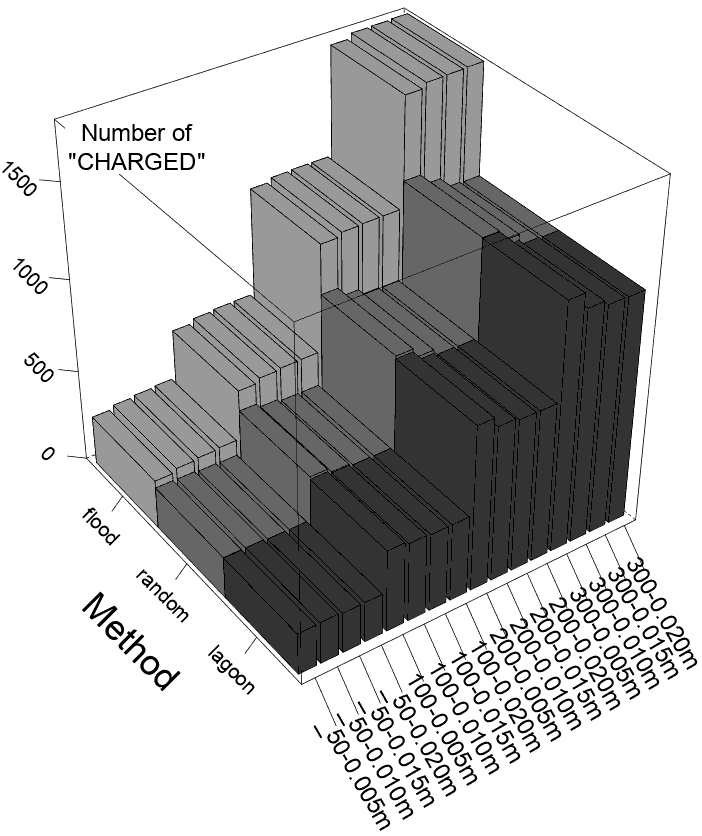
\includegraphics[width=\textwidth]{3dcharges2.png}
  \caption{3D bar chart for the "CHARGED" events.}
 \label{fig:recharges3d}
\end{figure}
\end{minipage}


The number of "CHARGED" events are lower in LaGOON, which can be seen from Table~\ref{tab:recharges} and from Figure~\ref{fig:recharges3d}.
The implication of the results is that the LaGOON has better energy efficiency and better transmission efficiency compared to the plain flooding protocol. 
Considering Algorithm~\ref{alg:algo1}, it can be seen that the space complexity is at the order of O(N) where N is the number of the nodes. 
Where as the time complexity to pick the best neighbor or "LaGOON", is just O(1), as fast table lookup mechanism can be used by utilizing node ids. 
Considering computational cost, this is not much different than picking a random node to forward. 
It can be said that the difference between LaGOON and random routing is insignificant. But when other factors are considered, 
like the number of "DROP" events, the LaGOON is better than random routing. In fact, LaGOON has the least "DROP" rate, and it is
the "most reliable" protocol compared to flooding and random routing. 
This difference can be seen from Table~\ref{tab:drops} and from Figure~\ref{fig:drops3d} more clearly,
where the number of the "DROP" is very low in LaGOON protocol compared to the plain flooding protocol and to the random routing.
This is expected as the LaGOON is keeping the minimum number of "forwarding" events. 
From Table~\ref{tab:drops} and from Figure~\ref{fig:drops3d} it can be seen that for increasing range and number of nodes (denser traffic), 
the difference between LaGOON and random routing grows. Denser traffic may 
help random routing for finding routes to the destination. But also increases the chance of choosing "charging" nodes and "circulating" packets 
unnecessarily longer in the network. Notably, the number of "DROP" events for the flooding protocol is very high since many copies of 
the same packet are generated and forwarded.

\vspace{-0.5cm}
\begin{minipage}[t]{0.42\textwidth}
\begin{table}[H]
\begin{center}
\caption{Comparison of "DROP" events}
\label{tab:drops}
\begin{adjustbox}{max width=\textwidth}
\begin{tabular}{|  >{\centering}m{1.2cm} | l || l | l | l | l |} 
\hline
& & \multicolumn{4}{c|}{\textbf{Number of Nano Nodes}} \\ \hhline{~|~|-|-|-|-}
\textbf{TX Range} & \textbf{Method} &  \textbf{50}  & \textbf{100} & \textbf{200} & \textbf{300} \tabularnewline \hline \hline
\multirow{3}{*}{0.005} & \textbf{lagoon} &      716 &     1668  &   3599  &     5498  \tabularnewline   \hhline{~|-|-|-|-|-}
                      & \textbf{random}  &      858 &     2013  &   4114  &     6156  \tabularnewline   \hhline{~|-|-|-|-|-}
                      & \textbf{flood}   &     2603 &     8512  &  28394  &    54689  \tabularnewline   \hline  \hline
\multirow{3}{*}{0.01}  & \textbf{lagoon} &      853 &     1608  &   3474  &     5325  \tabularnewline   \hhline{~|-|-|-|-|-}
                      & \textbf{random}  &     1002 &     2127  &   4316  &     6546  \tabularnewline   \hhline{~|-|-|-|-|-}
                      & \textbf{flood}   &     4220 &    14119  &  40593  &    79041  \tabularnewline   \hline  \hline
\multirow{3}{*}{0.015} & \textbf{lagoon} &      883 &     1524  &   3113  &     4797  \tabularnewline   \hhline{~|-|-|-|-|-}
                      & \textbf{random}  &     1043 &     2317  &   4626  &     7013  \tabularnewline   \hhline{~|-|-|-|-|-}
                      & \textbf{flood}   &     5955 &    17708  &  51303  &    89375  \tabularnewline   \hline  \hline
\multirow{3}{*}{0.02}  & \textbf{lagoon} &     900  &     1206  &   2589  &     4105 \tabularnewline   \hhline{~|-|-|-|-|-}
                      & \textbf{random}  &     1167 &     2524  &   5138  &     7867 \tabularnewline   \hhline{~|-|-|-|-|-}
                      & \textbf{flood}   &     6462 &    20492  &  65714  &   154610 \tabularnewline   \hline                    
\end{tabular}
\end{adjustbox}
\end{center}
\end{table}
\end{minipage}
\hfill
\begin{minipage}[t]{0.57\textwidth}
\begin{figure}[H]
\begin{center}
  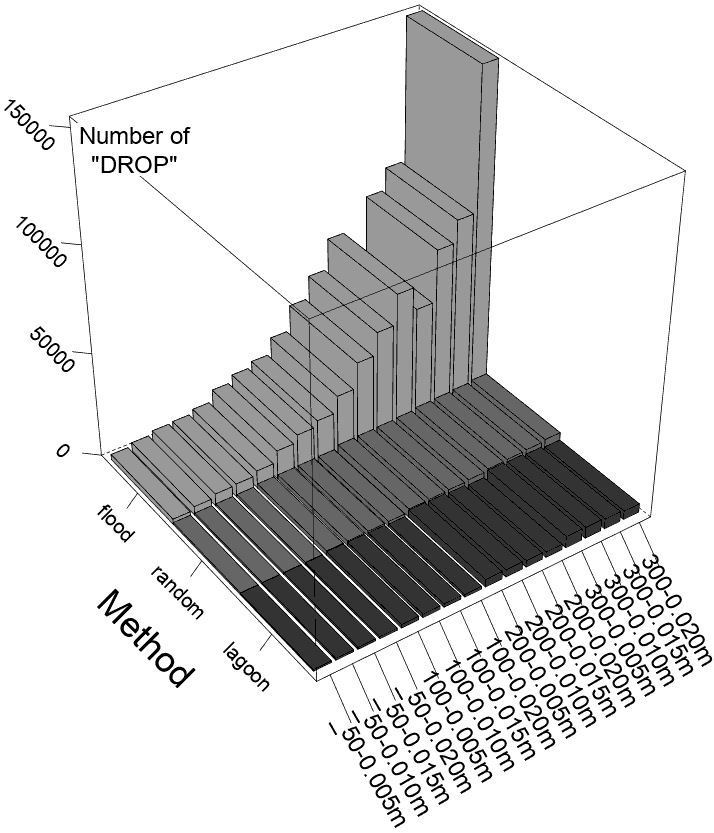
\includegraphics[width=\textwidth]{3ddrops2.png}
   \end{center}
   %\vspace{-0.8cm}
  \caption{3D bar chart for the "DROP" events.}
 \label{fig:drops3d}
\end{figure}
\end{minipage}



Table~\ref{tab:sends} and Figure~\ref{fig:sends3d} show the statistics about the number of "SEND" events. This measure is related to the "overall energy utilization performance" of 
the protocol. It also shows the "throughput" of the overall system in terms of successful packet generation and delivery. 
If nodes are, most of the time, in "charging" state, the number of "SEND" events will be low. 
The only reason for this is the bad routing decision. 
As it can be seen from Table~\ref{tab:sends} and from Figure~\ref{fig:sends3d}, LaGOON and random routing being almost similar in performance. 
But without looking at Table~\ref{tab:forwards} and at Figure~\ref{fig:forwards3d}, it can not be understood the difference between LaGOON and random routing. 
%
%
%

\vspace{2cm}

\begin{minipage}[t]{0.42\textwidth}
\begin{table}[H]
\begin{center}
\caption{Comparison of "SEND" events}
\label{tab:sends}
\begin{adjustbox}{max width=\textwidth}
\begin{tabular}{| >{\centering}m{1.2cm} | l || l | l | l | l |} 
\hline
& & \multicolumn{4}{c|}{\textbf{Number of Nano Nodes}} \\ \hhline{~|~|-|-|-|-}
\textbf{TX Range} & \textbf{Method} &  \textbf{50} & \textbf{100} & \textbf{200} & \textbf{300} \tabularnewline \hline \hline
\multirow{3}{*}{0.005} & \textbf{lagoon} &   1152 &     2360   &     4604  &    6871    \tabularnewline   \hhline{~|-|-|-|-|-}
                      & \textbf{random}  &   1102 &     2260   &     4488  &    6607    \tabularnewline   \hhline{~|-|-|-|-|-}
                      & \textbf{flood}   &    757 &     1183   &     1572  &    1911    \tabularnewline   \hline  \hline
\multirow{3}{*}{0.01}  & \textbf{lagoon} &   1215 &     2542   &     4946  &    7328    \tabularnewline   \hhline{~|-|-|-|-|-}
                      & \textbf{random}  &   1231 &     2415   &     4728  &    7070    \tabularnewline   \hhline{~|-|-|-|-|-}
                      & \textbf{flood}   &    643 &      831   &     1124  &    1419    \tabularnewline   \hline  \hline
\multirow{3}{*}{0.015} & \textbf{lagoon} &   1343 &     2790   &     5496  &    8131    \tabularnewline   \hhline{~|-|-|-|-|-}
                      & \textbf{random}  &   1319 &     2646   &     5150  &    7689    \tabularnewline   \hhline{~|-|-|-|-|-}
                      & \textbf{flood}   &    536 &      678   &      998  &    1194    \tabularnewline   \hline  \hline
\multirow{3}{*}{0.02}  & \textbf{lagoon} &   1463 &     2951   &     5900  &    8840    \tabularnewline   \hhline{~|-|-|-|-|-}
                      & \textbf{random}  &   1439 &     2888   &     5763  &    8626    \tabularnewline   \hhline{~|-|-|-|-|-}
                      & \textbf{flood}   &    445 &      599   &      828  &    1192    \tabularnewline   \hline                    
\end{tabular}
\end{adjustbox}
\end{center}
\end{table}
\end{minipage}
\hfill
\begin{minipage}[t]{0.57\textwidth}
\begin{figure}[H]
\begin{center}
  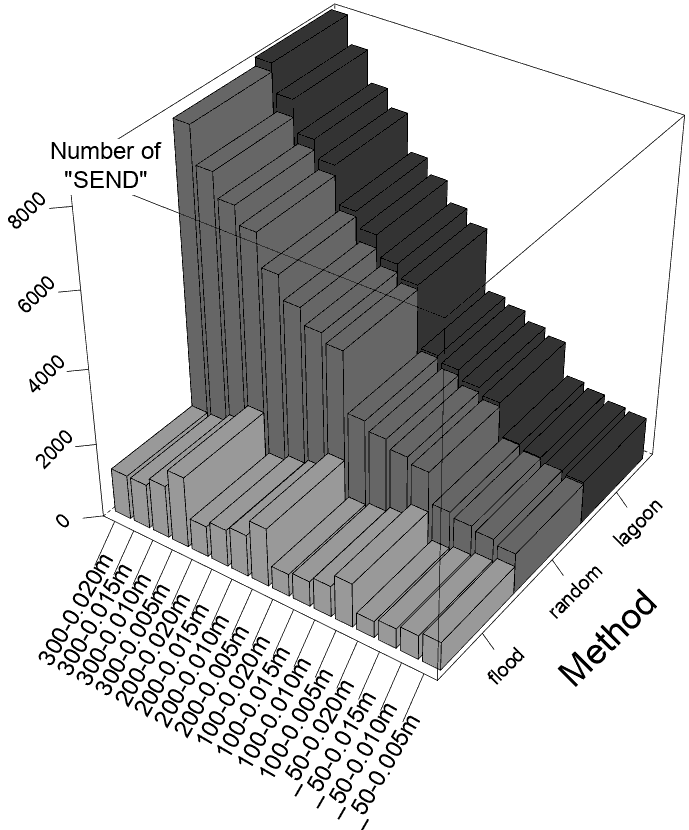
\includegraphics[width=\textwidth]{3dsends2.png}
   \end{center}
    %\vspace{-0.8cm}
  \caption{3D bar chart for the "SEND" events.}
 \label{fig:sends3d}
\end{figure}
\end{minipage}

\pagebreak

Table~\ref{tab:forwards} and Figure~\ref{fig:forwards3d} show again increasing difference between LaGOON and random 
routing as the transmission range gets further and the number of nodes increases. Basically for increased traffic LaGOON becomes better than random routing.
In other words, in the case of less number of nodes, choosing nodes for forwarding randomly may help, but when the traffic 
increases this way may be costly as it is explained in the previous paragraph. That is where LaGOON excels, by utilizing the minimalist way and adding little "heuristics" to routing decisions.


\begin{minipage}[t]{0.42\textwidth}
\begin{table}[H]
\begin{center}
\captionof{table}{Comparison of "FORWARD" events}
\label{tab:forwards}
\begin{adjustbox}{max width=\textwidth}
\begin{tabular}{| >{\centering}m{1.2cm} | l || l | l | l | l |} 
\hline
& & \multicolumn{4}{c|}{\textbf{Number of Nano Nodes}} \\ \hhline{~|~|-|-|-|-}
\textbf{TX Range} & \textbf{Method} &  \textbf{50} & \textbf{100} & \textbf{200} & \textbf{300} \tabularnewline \hline \hline
\multirow{3}{*}{0.005} & \textbf{lagoon} &     749 &     1344    &   2771   &     4157  \tabularnewline   \hhline{~|-|-|-|-|-}
                      & \textbf{random}  &     793 &     1536    &   3002   &     4452  \tabularnewline   \hhline{~|-|-|-|-|-}
                      & \textbf{flood}   &    1472 &     3467    &   8026   &    12554  \tabularnewline   \hline  \hline
\multirow{3}{*}{0.01}  & \textbf{lagoon} &     713 &     1127    &   2231   &     3351  \tabularnewline   \hhline{~|-|-|-|-|-}
                      & \textbf{random}  &     688 &     1266    &   2478   &     3677  \tabularnewline   \hhline{~|-|-|-|-|-}
                      & \textbf{flood}   &    1702 &     4020    &   8648   &    13249  \tabularnewline   \hline  \hline
\multirow{3}{*}{0.015} & \textbf{lagoon} &     550 &      820    &   1592   &     2442  \tabularnewline   \hhline{~|-|-|-|-|-}
                      & \textbf{random}  &     579 &      992    &   1981   &     2924  \tabularnewline   \hhline{~|-|-|-|-|-}
                      & \textbf{flood}   &    1892 &     4234    &   8811   &    13515  \tabularnewline   \hline  \hline
\multirow{3}{*}{0.02}  & \textbf{lagoon} &     402 &      511    &    938   &     1358  \tabularnewline   \hhline{~|-|-|-|-|-}
                      & \textbf{random}  &     425 &      701    &   1272   &     1859  \tabularnewline   \hhline{~|-|-|-|-|-}
                      & \textbf{flood}   &    2045 &     4331    &   8986   &    13536  \tabularnewline   \hline                    
\end{tabular}
\end{adjustbox}
\end{center}
\end{table}
\end{minipage}
\hfill
\begin{minipage}[t]{0.57\textwidth}
\begin{figure}[H]
\begin{center}
  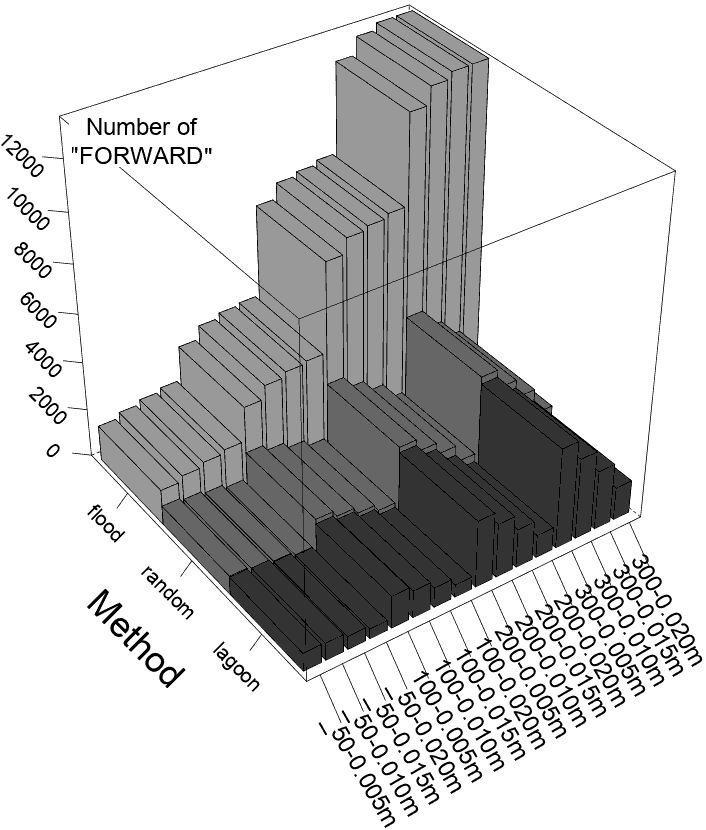
\includegraphics[width=\textwidth]{3dforwards2.png}
   \end{center}
  \caption{3D bar chart for the "FORWARD" events.}
 \label{fig:forwards3d}
\end{figure}
\end{minipage}


% 
% 
% \begin{table}[H]
% \begin{center}
% \caption{Comparison of "FORWARD" events}
% \label{tab:forwards}
% \begin{adjustbox}{max width=0.6\textwidth}
% \begin{tabular}{| >{\centering}m{1.2cm} | l || l | l | l | l |} 
% \hline
% & & \multicolumn{4}{c|}{\textbf{Number of Nano Nodes}} \\ \hhline{~|~|-|-|-|-}
% \textbf{TX Range} & \textbf{Method} &  \textbf{50} & \textbf{100} & \textbf{200} & \textbf{300} \tabularnewline \hline \hline
% \multirow{3}{*}{0.005} & \textbf{lagoon} &     716  &     1291    &    2628   &     3871  \tabularnewline   \hhline{~|-|-|-|-|-}
%                       & \textbf{random}  &     807  &     1416    &    2666   &     4210  \tabularnewline   \hhline{~|-|-|-|-|-}
%                       & \textbf{flood}   &    1284  &     3408    &    7928   &    12590  \tabularnewline   \hline  \hline
% \multirow{3}{*}{0.01}  & \textbf{lagoon} &     560  &      971    &    1980   &     3017  \tabularnewline   \hhline{~|-|-|-|-|-}
%                       & \textbf{random}  &     662  &     1178    &    2192   &     3514  \tabularnewline   \hhline{~|-|-|-|-|-}
%                       & \textbf{flood}   &    1825  &     4033    &    8591   &    13217  \tabularnewline   \hline  \hline
% \multirow{3}{*}{0.015} & \textbf{lagoon} &     504  &      737    &    1419   &     2184  \tabularnewline   \hhline{~|-|-|-|-|-}
%                       & \textbf{random}  &     511  &      988    &    1819   &     2778  \tabularnewline   \hhline{~|-|-|-|-|-}
%                       & \textbf{flood}   &    1877  &     4181    &    8833   &    13530  \tabularnewline   \hline  \hline
% \multirow{3}{*}{0.02}  & \textbf{lagoon} &     388  &      439    &     818   &     1222  \tabularnewline   \hhline{~|-|-|-|-|-}
%                       & \textbf{random}  &     414  &      702    &    1210   &     1802  \tabularnewline   \hhline{~|-|-|-|-|-}
%                       & \textbf{flood}   &    2117  &     4355    &    9012   &    13661  \tabularnewline   \hline                    
% \end{tabular}
% \end{adjustbox}
% \end{center}
% \end{table}
% 
% 
% 
% 
% \begin{figure}[H]
% \begin{center}
%   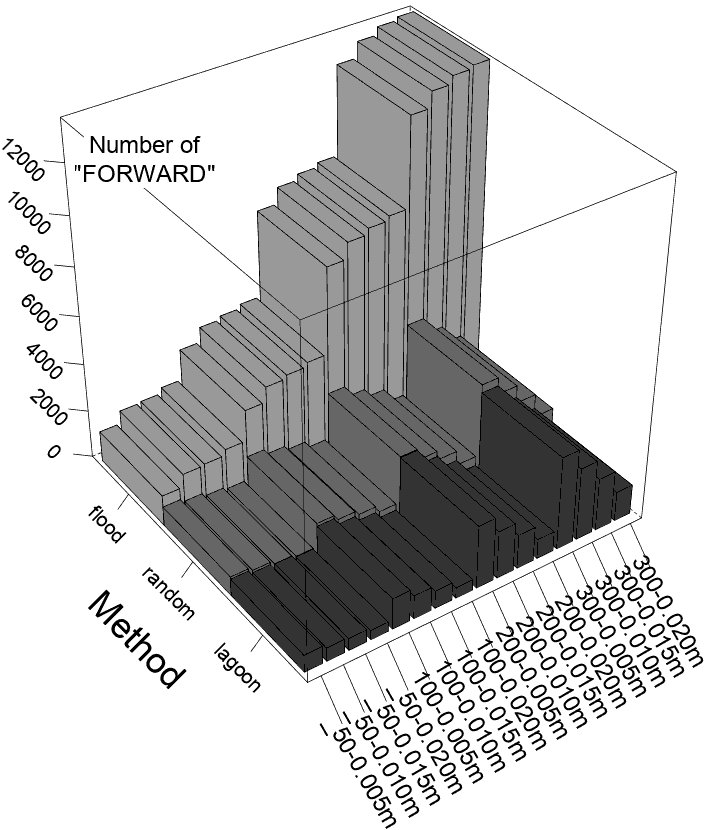
\includegraphics[width=0.6\textwidth]{3dforwards.png}
%    \end{center}
%   \caption{3D bar chart for the "FORWARD" events.}
%  \label{fig:forwards3d}
% \end{figure}




In general, in all the benchmarks, proposed LaGOON protocol performed very well, without compromising among energy saving, 
reliability, and computational cost for routing decisions. The results are justified with the statistical analysis in which
"ANOVA analysis" (whether means are different) and
"Tukey Honest Significant Differences" (which mean differences are statistically significant) tests are applied to verify the differences in mean values.
One of the highlights of the LaGOON protocol is the fact that having 
such a good level of efficiency with a little computational cost can give space to further optimizations. 

Flexibility is another 
good feature of the protocol. Not only the protocol is topology independent, but also it can be customized for 
handling different mobility models. The "evolving learning" mechanism for route discovery is carried out in a distributive manner.
In the implementation used in this thesis for the experiments, control packets are not included. However, for mobile networks, additional
control packets can be added easily for broadcasting position changes. This can help LaGOON for faster route discovery. In the same manner, 
hierarchical position information can also be added to LaGOON by imposing restrictions in the routing.
 
% 
% % 
% %
% % 
% \begin{figure}[!htbp]
% \begin{center}
%   \includegraphics[width=0.6\textwidth]{tot_energy_cons.png}
%    \end{center}
%   \caption{Total Energy consumption of the network TunableMAC}
%  \label{fig:tunableMAC1}
% \end{figure}
% % 
% %
% %
% 
% % 
% %
% % 
% \begin{figure}[!htbp]
% \begin{center}
%   \includegraphics[width=0.6\textwidth]{tot_energy_cons2.png}
%    \end{center}
%   \caption{Total Energy consumption of the network TunableMAC}
%  \label{fig:tunableMAC2}
% \end{figure}
% % 
% %
% %
% 







%%%%%%%%%%%%%%%%%%%%%%%%%%%%%%%%%%%%%%%%%%%%%%%%%%%%%%%%%%%%%%%%%%%%%%%%%%%%%%%%%%%%%%%%%%%%%%%%%%%%%%%%%%%%%%%%%%%%%%%%%%%%%
\newpage
\section{Contributions of the Thesis to Routing}\label{scontribrouting}

In this section, the contributions of the thesis to the routing research will be listed. As a theoretical contribution,
the gaps in the energy aware routing research will be listed and discussed. The discussions on the proposed routing algorithm
will be presented as a framework for a simple and energy aware routing.

While the routing is very extensively researched for WSNs, still for WNSNs there are open issues and challenges.
In nanonetworks still, there is no standard routing protocol, as in the case of WSNs. In WSNs there are well known 
routing protocols like AODV, DSR. However, in the case of nanonetworks the routing protocols are in the preliminary stage.
There are many reasons for that. One reason is the peculiarities of the THz frequency communication. In THz communication, 
not only MAC layer needs to be customized, but also antenna technologies should be customized too~\cite{akyildiz2014}. 

On the other hand, still, there are gaps and issues that can be further elaborated in the routing related research for WSNs.
Statistical modeling of the packet arrival is one of them. In fact, the issue is rooted in considering the "user (sensor) behavior". 
The sensor nodes, depending on the application of the deployed WSN, can exhibit a peculiar way of transmission patterns. For example
in the temperature sensing, the transmission may obey certain communication patterns,
if the system reports temperature every 5 minutes or reports the temperature change during the day when there is one or two Celsius
deviance. These type of "user behavior" can be modeled statistically in the simulators. One of the benefits that such study can provide
is the customized MAC protocol in which duty cycling can be adjusted to the "user behavior" or can learn the "user behavior" patterns.
Such enhancements can save energy in the WSNs. Certain assumptions regarding the existing statistical models for the system attributes 
should be validated before applying them to the simulations.
The paper~\cite{doddapaneni2015} is one of the good examples of the perils of accepting conventional models without verification.
The study focused on the statistical modeling of the packet arrivals, specifically for the cluster heads in WSNs. 
While authors stated that the exponential packet inter-arrival distribution holds only under special conditions 
involving small scale WSNs (10-15 nodes) and sparse traffic, they also explained the trade-off between energy consumption and average 
end-to-end delay of the system. The study emphasized the importance of the statistical validation of the distribution types regarding 
the packet inter-arrivals.

Another important issue is the customized routing algorithm that combines "battery awareness" and "duty cycling". 
Battery aware routing topic is proposed and studied in~\cite{ma2005} and comprehensive taxonomy on the duty cycling is given 
in~\cite{carrano2014}. Batteries can "self-recover" if the current draw can be kept in the specific margins according to the 
type of the battery. Energy aware routing algorithm combined with the appropriate MAC layer can interleave duty cycling to
allow battery self-recovery. Energy aware MAC layer can also decide on the splitting of the frame into smaller sizes for avoiding
current over-draw. These two techniques can keep the battery in safe margins allowing it to self-recover. However, in the literature
no such technique is proposed. One important factor in researching such a technique is the battery models that the WSN simulators offer.
Mostly simulators assume simple "linear" battery model, in which every transmission and reception require the same amount of energy.
However, this assumption is so limiting and simplistic. 


Although the thesis is pointing out such issues listed above, they are not included in the implementations of this study. 
However, as a theoretical contribution, discussions on these issues are offered as conceptual frameworks.
The practical contributions of the thesis are mainly focused on the routing,
since the idea of transmissions being the most energy consuming activities is embraced as a main premise in the thesis.
The proposed routing algorithm is itself a contribution for the routing research related to the WNSNs,
when the number of existing implementations is considered. In Table~\ref{tab:litsur}
existing approaches related to the WNSNs are listed and compared.

\vspace{-0.5cm}
\renewcommand{\arraystretch}{1.2}%
\begin{table}[H]
\begin{center}
\caption{Comparison of existing routing algorithms for WNSNs (as of 2018).}
\label{tab:litsur}
\begin{adjustbox}{max width=\textwidth}
\begin{tabular}{| l || l |} 
\hline
\rowcolor{lightgray}
\textbf{Paper} & \textbf{Contribution Summary} \tabularnewline
\hline \hline
 \cellcolor{lightgray} zhou2012~\cite{zhou2012}       &  {\parbox[t]{14cm}{PHY layer and pair-to-pair routing. Not very energy efficient.}} \tabularnewline \hline
 \cellcolor{lightgray} yu2015~\cite{yu2015}           &  {\parbox[t]{14cm}{Channel-aware routing protocol. 1D topology. Energy not considered.}} \tabularnewline \hline
 \cellcolor{lightgray} liaskos2015~\cite{liaskos2015} &  {\parbox[t]{14cm}{CORONA. Minimize hop count. 2D Grid topology. Energy considered. "Anchor" nodes.}}\tabularnewline \hline
 \cellcolor{lightgray} liaskos2016~\cite{liaskos2016} &  {\parbox[t]{14cm}{Peer-to-peer routing.  2D Grid topology. Node classification based on past statistics.}} \tabularnewline \hline
 \cellcolor{lightgray} tairin2017~\cite{tairin2017}   &  {\parbox[t]{14cm}{Hierarchical AODV. Energy considered.}} \tabularnewline \hline
 \cellcolor{lightgray} afsana2018~\cite{afsana2018}   &  {\parbox[t]{14cm}{Channel aware energy conserving protocol. Hybrid clustering of the nanonodes and centralized scheduling.}} \tabularnewline \hline\hline
 \rowcolor{green}
 lagoon       &  {\parbox[t]{12cm}{Lightweight energy aware protocol. Minimize hop count. Topology independent.}} \tabularnewline \hline
\end{tabular}          
\end{adjustbox}        
\end{center}           
\end{table}            
\renewcommand{\arraystretch}{1}%



In the proposed routing algorithm, the setup was not necessary, although it can be applied to speed up the "route learning" process.
The sensors nodes do not have to follow certain flooding period. However, any node that does not have any path information in its routing table,
individually, can do flooding. 
This feature makes the algorithm very lightweight and flexible,
both in computation and in transmission.
In some protocols, this phase is important and specialized packets need to be transmitted. Even in some protocols time synchronization 
is essential as the network limits the setup time according to the time limit set by the network administer. Such protocols may have
higher energy consumption due to the extra transmissions for set up packets.
Especially in WNSNs energy is very limited and such protocols can not be used.
Compared to other proactive algorithms (table driven, e.g. DSDV), in which route discovery is done before the request and global routing tables 
are distributed, LaGOON does not proceed in this way. In the proposed LaGOON protocol routing tables are local and evolve 
with the time as the new information is received. Also contrary to the reactive routing algorithms (on demand, e.g. AODV), LaGOON does not request route
discovery on demand. However, nodes route packets according to the local routing they have so far. In the case of "empty routing" table, 
LaGOON can be customized to initiate routing with flooding or by choosing a random neighbor. 
Node failures and node mobility can be solved with periodic controlled flooding.

Another contribution of the thesis is the "directional" version of the LaGOON protocol, which is explained in Chapter~\ref{clagoon}.
The flexibility of this protocol is based on the directional MAC and physical layers. It requires minor changes to be adapted to directional
communication. The routing proceeds as in the case of omnidirectional case, with the addition of direction information recorded in the routing tables.
The algorithm can accommodate an arbitrary number of directional antennas. The implementation of this version was not included in this thesis.
One of the reasons was the capabilities of the available simulators did not cover directional antenna simulations.













\newpage
%%%%%%%%%%%%%%%%%%%%%%%%%%%%%%%%%%%%%%%%%%%%%%%%%%%%%%%%%%%%%%%%%%%%%%%%%%%%%%%%%%%%%%%%%%%%%%%%%%%%%%%%%%%%%%%%%%%%%%%%%%%%%
\chapter{Directional Antenna}\label{cdantenna}

In the previous section, the proposed energy aware LaGOON protocol is discussed in detail by highlighting its energy aware properties. 
An energy aware routing algorithm can save energy in many ways. It can forward messages over shortest paths reducing the number of transmissions.
The routing method in doing this, it can also try to keep the overhead associated to the mechanism low. Namely, control messages specific to the routing itself.
Routing algorithm can also be "battery aware". The batteries can be depleted faster if the current draw is very high for transmission. The "battery aware"
routing can use packet division and duty cycling in such ways that the continuous high current draw can be optimized to allow self-recharging of the battery.
But still, with the use of omnidirectional antennas, the signal will be transmitted all around. With the exception of "flooding", this transmission pattern is not necessary.
By "broadcasting" the signal all around, omnidirectional antennas consume higher levels of energy and introduce limits to the energy savings of the "routing" algorithm.
On the other hand, directional antennas for the same transmission ranges, they consume less energy for communication and they contribute to the energy savings from 
the directional antennas.
In this sense, it is desirable to establish synergy between the energy aware routing and the directional antenna.

This section will present the second method that is proposed related to the energy problem in WSNs, which involves the use of directional (directed, sectored, etc...) antennas.
In the following subsections little overview of the important antenna characteristics, comments on the works related to the use of directional antennas in WSNs, and 
performance characteristics of the designed directional microstrip patch antenna array will be presented.


\newpage
%%%%%%%%%%%%%%%%%%%%%%%%%%%%%%%%%%%%%%%%%%%%%%%%%%%%%%%%%%%%%%%%%%%%%%%%%%%%%%%%%%%%%%%%%%%%%%%%%%%%%%%%%%%%%%%%%%%%%%%%%%%%%
\section{Antenna Basics}\label{santbas}
According to the IEEE Standard Definitions of Terms for Antennas document (IEEE
Std 145–20133)~\cite{ieee2013}, antenna defined as: 
%
%
\begin{quote}
\enquote{That part of a transmitting or receiving system that is designed to radiate or to receive
electromagnetic waves.}
\end{quote}
\vspace{-5mm}
%
%
Antennas come in various types and geometries. In~\cite{balanis2016} various types of antennas listed, mainly according to the geometry and architecture:  
\begin{enumerate}
\setlength\itemsep{0em}
\item Wire 
\item Aperture
\item Microstrip
\item Array
\item Reflector
\item Lens
\end{enumerate}
%
Figure~\ref{fig:antennas} below presents a classification of the antennas used in communication systems based on the radiation technology.
% 
%
%
\begin{figure}[!htbp]
 \begin{center}
  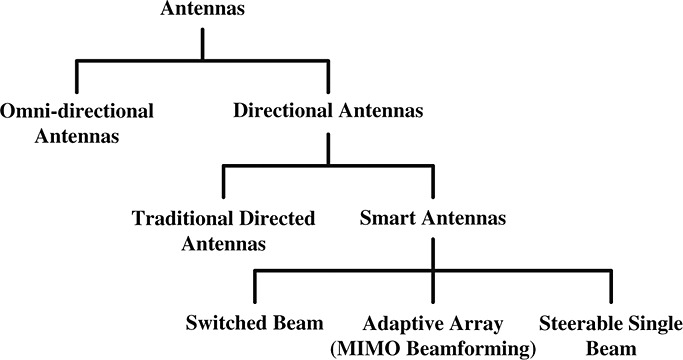
\includegraphics[width=0.7\textwidth]{antennas.png}
 \end{center}
 \caption{Classification of antennas based on the technology utilized for directing signals. (Source:~\protect\cite{dai2011})}
  \label{fig:antennas}
\end{figure}
% 
%
%
%
\newpage
In this thesis hybrid type is used, in which microstrip antennas are combined in 2 by 2 array to form directional antenna. Microstrip antennas
basically consist a dielectric substrate sandwiched between a metallic patch and a ground layer. Various types of substrates are used, which should be
selected according to the frequency and performance requirements. The article~\cite{khan2012} presents discussions on the performance 
effects of the substrates that can be used for microstrip antennas.
As it is stated in~\cite[pp.~25-105]{balanis2016}, there are many parameters that 
can "describe" the performance of an antenna. Detailed discussions on the various characteristics of antennas can be found in textbooks such as~\cite{balanis2016} and~\cite{pozar2011}.
The thesis~\cite{whyte2008} presents substantial material on the theory and practice of the antenna design, specific to WSN applications.

For this thesis the focus of interest was on the "gain" and the "return loss" (S11: S-parameters~\cite{atheory-s11}). 
"Efficiency" of an antenna is a multidimensional concept. Basically, it considers losses related to the input terminal of the antenna. 
These losses can be grouped as "reflections" and "conduction and dielectric" losses. Reflections are due to the mismatch between 
transmission circuitry (brings current to the antenna) and the antenna. Conduction and dielectric losses are due to resistance~\cite[p.~60]{balanis2016}.


Voltage Standing Wave Ratio (VSWR) is a performance measure that is related to losses due to the mismatch between antenna and the transmission line.
It has a value that is either greater than 1 or equal to 1. VSWR value 1 means a perfect match between the antenna and the transmission line. 
Values that are greater than 1 signify greater losses due to mismatch~\cite{atheory-imp}. VSWR is a function of the reflection coefficient 
known as S11 (return loss) which is represented by $\Gamma$ in the formulas. Generally, S11 is given in dB. The formula for S11 represented in dB is
given in equation~\ref{eq:s11db} below:

\begin{equation}
\text{S11}~=~-20\log\abs{\Gamma}~(\text{dB}) \label{eq:s11db}
\end{equation}
%
Reflection coefficient quantifies the power reflected from the antenna.
The relationship between VSWR and S11 can be given in equation~\ref{eq:s11} below~\cite{atheory-vswr}:

\begin{equation}
\text{VSWR}~=~\frac{1+\abs{\Gamma}}{1-\abs{\Gamma}} \label{eq:s11}
\end{equation}
%
\newpage
Table~\ref{tab:vswr} shows the relationship among VSWR, S11, and reflected power numerically~\cite{atheory-vswr}. 
%
%\vspace{-0.5cm}
\renewcommand{\arraystretch}{1.2}%
\begin{table}[H]
\begin{center}
\caption{Numerical relationship among VSWR, S11, reflected power percentage, and reflected power in dB. (Source:~\protect\cite{atheory-vswr})}
\label{tab:vswr}
\begin{adjustbox}{max width=\textwidth}
\begin{tabular}{| >{\centering}m{3cm} | >{\centering}m{3cm} | >{\centering}m{4cm} | >{\centering}m{4cm} |}
\hline
\rowcolor{lightgray}
\textbf{VSWR} & \textbf{$\Gamma$~(S11)} & \textbf{Reflected Power(\%)} & \textbf{Reflected Power(dB)} \tabularnewline \hline \hline 
1.0 & 0.000 & 0.00 & $-\infty$ \tabularnewline \hline
2.0 & 0.333 & 11.1 & -9.55   \tabularnewline \hline
4.0 & 0.600 & 36.0 & -4.44   \tabularnewline \hline
8.0 & 0.778 & 60.5 & -2.18   \tabularnewline \hline
20.0 & 0.905 & 81.9 & -0.87  \tabularnewline \hline
50.0 & 0.961 & 92.3 & -0.35  \tabularnewline \hline
\end{tabular}
%\\[1.0] %You can adjust how far below the table the text should appear
\end{adjustbox}
\end{center}
\end{table}
\renewcommand{\arraystretch}{1}%
% 
% 
%

"Gain" (relative gain) is, mostly, stated in reference to isotropic antenna. Isotropic case represents ideal case of an antenna in which the radiation of signals are spherical 
(equal in all directions). More technical explanation can be given by quoting Balanis~\cite{balanis2016}:
%
%
\begin{quote}
\enquote{Gain of an antenna (in a given direction) is defined as the ratio of the intensity, in a given direction, 
to the radiation intensity that would be obtained if the power accepted by the antenna were
radiated isotropically. The radiation intensity corresponding to the isotropically radiated power is
equal to the power accepted (input) by the antenna divided by 4$\pi$.
}
\end{quote}
%\vspace{-5mm}
%
%
Figure~\ref{fig:antenna-coor} depicts the antenna coordinate system that is helpful for explaining the concept of "gain".
% 
%
%
\begin{figure}[!htbp]
 \begin{center}
  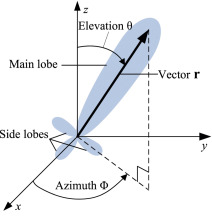
\includegraphics[width=0.5\textwidth]{antenna-coor.png}
 \end{center}
 \caption{Antenna Coordinate system. (Source:~\protect\cite{xli2015})}
  \label{fig:antenna-coor}
\end{figure}
% 
%
%
%
Directional antennas, when they radiate they form a "beam" like radiation pattern, instead of a "sphere" which isotropic antenna supposed to form.
This beam, which is named as "main lobe" can be seen in Figure~\ref{fig:antenna-coor}.  

The equation~\ref{eq:gain}~\cite[p.~62]{balanis2016} describes gain (relative to isotropic) in mathematical format, which is dimensionless.
In the equation~\ref{eq:gain}, $U(\theta, \phi)$ represents "intensity" in a given direction, which can be defined as 
"the power radiated from an antenna per unit solid angle"~\cite[p.~37]{balanis2016}. 
\begin{equation}
\text{Gain}~=~\frac{4\pi U(\theta, \phi)}{\text{P$_{in}$(lossless isotropic source)}} \label{eq:gain}
\end{equation}
% % 
% The antenna efficiency (or radiation efficiency) can be written as the ratio of the radiated power to the input power of the antenna:
% \begin{equation}
% \Epsilon_R~=~\frac{P_{radiated}}{P_{input}} \label{eq:reff}
% \end{equation}
% 
% However, more often a single number is quoted the gain is the 'peak gain' over all directions. Antenna Gain (G) can be related to directivity (D) and antenna efficiency by:
% \begin{equation}
% \text{Gain}~=~\frac{4\pi U(\theta, \phi)}{\text{P$_{in}$(lossless isotropic source)}} \label{eq:gain}
% \end{equation}

\newpage

In order to show the gain relationship among different types of antennas, in Figure~\ref{fig:iso-omni-dir},
radiation patterns of isotropic, omnidirectional, and directional antennas are depicted. In the figure, typical gain values are given in 
dBi (unit of gain as deciBel relative to the isotropic radiator).
% 
%
%
\begin{figure}[!htbp]
 \begin{center}
  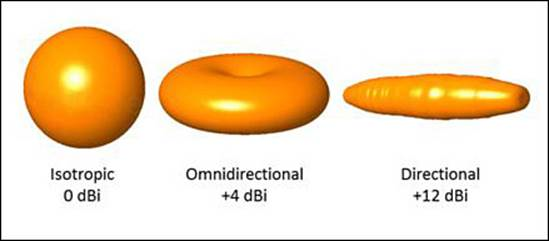
\includegraphics[width=0.8\textwidth]{iso-omni-dir.png}
 \end{center}
 \caption{Radiation patterns of isotropic (theoretical), omnidirectional (typical), and directional (typical) antennas and typical gain values. (Source:~\protect\url{http://apprize.info/network/ccna/ccna.files/image102.jpg})}
  \label{fig:iso-omni-dir}
\end{figure}
% 
%
%
%
%%%%%%%%%%%%%%%%%%%%%%%%%%%%%%%%%%%%%%%%%%%%%%%%%%%%%%%%%%%%%%%%%%%%%%%%%%%%%%%%%%%%%%%%%%%%%%%%%%%%%%%%%%%%%%%%%%%%%%%%%%%%%
\newpage
\section{Research in Directional Antenna}\label{santresearch}
%%%%%%%%%%%%%%%%%%%%%%%%%%%%%%%%%%%%%%%%%%%%%%%%%%%%%%%%%%%%%%%%%%%%%%%%%%%%%%%%%%%%%%%%%%%%%%%%%%%%%%%%%%%%%%%%%%%%%%%%%%%%%
% Always remembering energy efficiency:
% Firstly a bit of WNSNs : Already some stuff here
% WSN routing stuff, especially AODV things
% Antenna stuff
% WSN + directional antenna thesis and papers at:
% /my_hd2/my_dir/my_courses/METU/SEES/MSc-Thesis-stuff/my/papers/WSN/directional-antenna/thesis
%
%
%%%%%%%%%%%%%%%%%%%%%%%%%%%%%%%%%%%%%%%%%%%%%%%%%%%%%%%%%%%%%%%%%%%%%%%%%%%%%%%%%%%%%%%%%%%%%%%%%%%%%%%%%%%%%%%%%%%%%%%%%%%%%
%\vspace{-0.cm}

Research for utilization of directional antennas in sensor nodes is developed in to two branches. While several studies focus on the 
performance characteristics of the physical antenna design, others emphasize the development of specialized routing and/or specialized MAC protocols.

Since in sensor networks most of the energy is consumed for communication, 
optimization of the transmissions and receptions can improve sensor battery lifetime along with the overall network lifetime. In that sense, directional antennas
offer optimization at the local level (involving only the sensor node) and also at the global level (overall network lifetime).
Considering the architecture of a sensor node, it can also be said that
directional antennas are one of the optimization technologies at the hardware level~\cite{winters2006, jamshed2018, rault2014}.
They have advantages over the omnidirectional antennas, such as higher gain, less interference, spatial reuse, longer transmission range, security, and 
less power consumption~\cite{dai2011, georgiou2015, curiac2016, cisco}. 
However, the directional antennas are not widely used in WiFi communication today. Mostly omnidirectional antennas are utilized in personal computers.
This is because, originally the IEEE 802.11 (physical and MAC level specifications for wireless communication) standard designed for omnidirectional antennas in 1997. 


On the other hand, many studies tried to extend this standard and implemented experimental support for directional antennas like in~\cite{ko2000} and in~\cite{zhu2006}.
Consequently, the first MIMO (Multiple Input Multiple Output) support is included in the IEEE 802.11n standard, 
in which multiple antennas are utilized for achieving higher data rates through aggregation,
compared to the SISO (Single Input Single Output), MISO (Multiple Input Single Output), SIMO (Single Input Multiple Output) systems. 


\newpage
In Figure~\ref{fig:mimo}, the possibility of increasing the data rate in MIMO systems is depicted compared to other types of systems. 

% 
%
%
\begin{figure}[!htbp]
 \begin{center}
  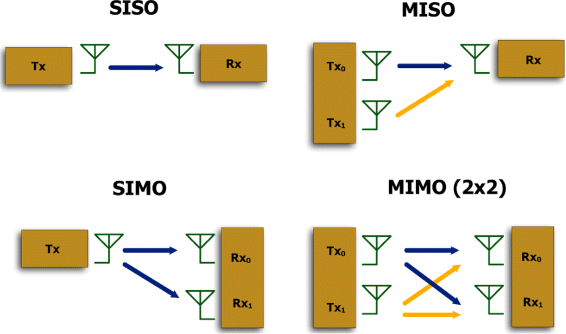
\includegraphics[width=0.8\textwidth]{mimo-multipath.png}
 \end{center}
 \caption{Data rate aggregation in a MIMO antenna system compared to other systems. (Source:~\protect\cite{bennani2016})}
  \label{fig:mimo}
\end{figure}
% 
%
%
%


Data can be divided and transferred through many lines simultaneously in the MIMO systems. Both transmission and reception can benefit from the multi-channel communication
without requiring extra power.


After that, first support for directional antennas came with the IEEE 802.11ac standardization of the beamforming property in 2008. 
A brief comparison of various IEEE standards for WiFi communication can be seen in Table~\ref{tab:ieee-wf}. 


%
%\vspace{-0.5cm}
\renewcommand{\arraystretch}{1.2}%
\begin{table}[H]
\begin{center}
\caption{IEEE WiFi standards. (Source:~\protect\cite{ferreira2016,ieee-wifi})}
\label{tab:ieee-wf}
\begin{adjustbox}{max width=\textwidth}
\begin{tabular}{| >{\centering}m{3cm} | >{\centering}m{3cm} | >{\centering}m{4cm} | >{\centering}m{4cm} |}
\hline
\rowcolor{lightgray}
\textbf{IEEE Standard} & \textbf{Frequency (GHz)} & \textbf{Bandwidth (MHz)} & \textbf{Max Data Rate (Mbit/s)} \tabularnewline \hline \hline 
802.11   & 2.4 & 20 & 2      \tabularnewline \hline
802.11b  & 2.4 & 20 & 11      \tabularnewline \hline
802.11a  & 5   & 20 & 54      \tabularnewline \hline
802.11g  & 2.4 & 20 & 54      \tabularnewline \hline
802.11n  & 2.4, 5 & 20,40  & 600      \tabularnewline \hline
802.11ac & 5  & 20, 40, 80, 160 & 6930      \tabularnewline \hline
802.11ad & 60000 & 2160 & 6760 \tabularnewline \hline
802.11ah & 0.9 & 1–16 & 347 \tabularnewline \hline
\end{tabular}
\end{adjustbox}
\end{center}
\end{table}
\renewcommand{\arraystretch}{1}%






In thesis~\cite{bian2009}, performance improvements in ad hoc networks with directional antennas topic was studied. 
The author pointed out the current weakness of the IEEE 802.11
Distributed Coordination Function and proposed solution based on the use of directional antennas. 
The idea was to use directional antennas in accordance with the carrier sensing threshold adjustments and power control for transmissions 
with a proposed MAC protocol for performance improvements. The thesis proposed novel way in achieving this idea by considering 
heterogeneity (nodes with omnidirectional and directional antennas) of the sensor nodes. The simulations in the thesis considered standard
IEEE 802.11 Directional Virtual Carrier Sensing (DVCS) MAC protocol, the IEEE 802.11b (improved version of the IEEE 802.11 with 11 Mbit/s throughput), 
and the proposed version of the DVCS (PVDVCS, Power Controlled Directional Virtual Carrier Sensing).
The thesis reported that PCDVCS achieved 99.3\% increase in throughput compared to the IEEE 802.11b and 35\% increase over DVCS. 
Also, PCDVCS  achieved reduced power consumption of 83\% over the IEEE 802.11b and 64\% compared to DVCS.

In~\cite{kranakis2012}, the author presents interesting comparisons on the capacity of sensor networks ($n$ identical nodes, each transmitting $W$ bits per second) 
using directional and omnidirectional antennas. 
The paper~\cite{gupta2000} calculated the capacity of the network using omnidirectional antennas and gave the formula as it is shown in equation~\ref{eq:omni-cap} below: 
\begin{equation}
\sqrt{\frac{1}{2\pi}}W\sqrt{n}~\text{bits per second}\label{eq:omni-cap}
\end{equation}

On the other hand, authors in~\cite{yi2003} calculated the capacity of the network using directional antennas (with transmission beam of~$\alpha$ and receiving beam width of~$\beta$) 
and gave the formula as it is shown in equation~\ref{eq:dir-cap} below: 
\begin{equation}
\sqrt{\frac{2\pi}{\alpha\beta}}W\sqrt{n}~\text{bits per second}\label{eq:dir-cap}
\end{equation}

As it can be seen from the equations~\ref{eq:omni-cap} and~\ref{eq:dir-cap}, the capacity of a network with directional antennas, can be increased by using arbitrary
values for the $\alpha$ and~$\beta$. The author in the same talk (\cite{kranakis2012}) goes further in comparing the energy consumption of omnidirectional and directional antennas by
introducing a parametric framework based on the range and the transmission beam angle of the antennas. The talk proposes that the energy consumption ($E$) of an antenna is related to its 
range ($R$) and to its transmission beam ($\alpha$). This proportional relationship is shown with the equation~\ref{eq:eng-cons} given below:
\begin{equation}
E \propto \frac{\alpha}{2} \cdot R^2 ~\text{(For omnidirectional $\alpha$ = 2$\pi$)} \label{eq:eng-cons}
\end{equation}

Considering the same energy amount given to each type of antenna as $E$, the expression for the relationship among energy, range, and transmission beam angle can be given in equation~\ref{eq:range} below:
\begin{equation}
R \propto \sqrt{\frac{2 E} {\alpha}}~\text{(For omnidirectional $\alpha$ = 2$\pi$)} \label{eq:range}
\end{equation}

The implication of the equation~\ref{eq:range} is that, for the same energy amount, directional antenna with narrower transmission beam can reach further distances.
It can also be concluded that for the fixed range, the directional antenna spends less energy, since the transmission beam angle is less than $2\pi$. 
Total energy saving can be calculated by summing up all the savings from each node in the WSNs. For large WSNs with hundreds of sensor nodes the energy 
saving can be huge if directional antennas are used. This concept is visualized in Figure~\ref{fig:comm-cover} below, in which
the communication range difference between omnidirectional and directional antennas 
is depicted. 
\vspace{-0.1cm}
% 
%
%
\begin{figure}[!htbp]
 \begin{center}
  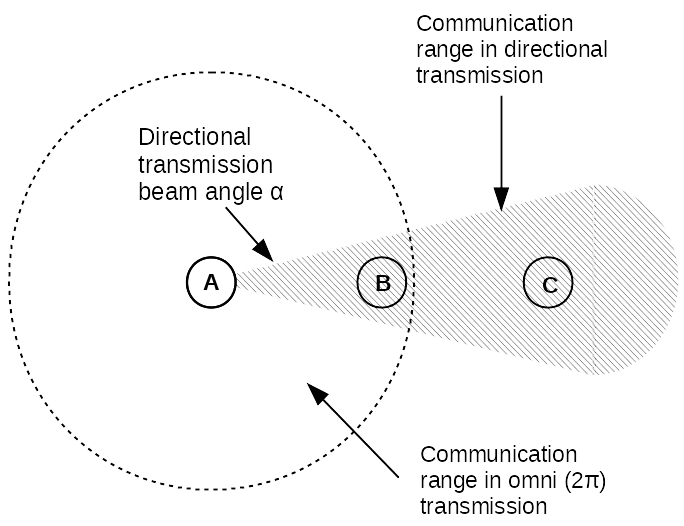
\includegraphics[width=0.7\textwidth]{comm-cover.png}
 \end{center}
 \caption{Comparison of the transmission coverage of the omnidirectional and the directional antennas. (Source:~\protect\cite[p.~308]{corderio2006})}
  \label{fig:comm-cover}
\end{figure}
% 
%
%
%

\newpage

In the figure, the transmission ranges are shown for equal energy consumption.  
Transmission from sensor node A to B can be achieved with lower energy consumption in the case of directional antenna.
However for transmission from A to C, omnidirectional antenna should consume greater energy compared to the directional antenna.
While directional antennas can have a more focused signal beam and greater ranges in signal transmission requiring the same amount of energy, 
omnidirectional antennas send the signal all around with smaller range. This way directional antennas can be more frugal in energy consumption for the required range.


Figure~\ref{fig:spatial-reuse} depicts the visual comparison of the spatial reuse differences between 
omnidirectional and directional antennas. Spatial reuse is higher in the case of the directional antennas as more than one communication link
can be formed at the same time. However in the case of omnidirectional antenna, when two nodes are in communication, all the nodes in the range 
has to be silenced.
\vspace{-0.2cm}
% 
%
%
\begin{figure}[!htbp]
 \begin{center}
  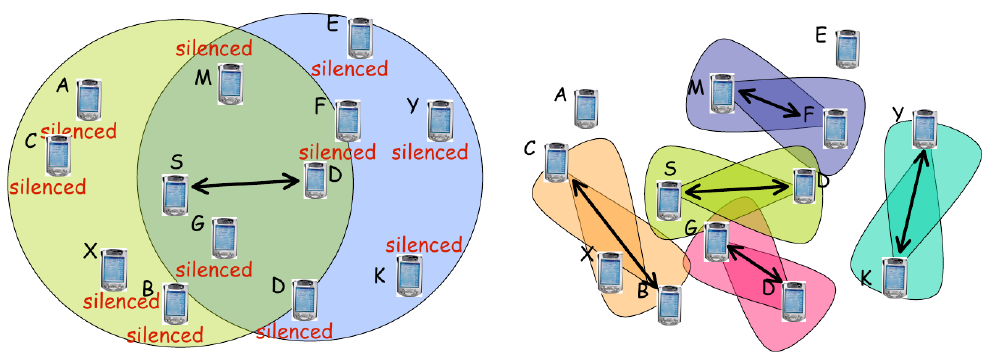
\includegraphics[width=0.95\textwidth]{spatial-reuse.png}
 \end{center}
 \caption{Comparison of the omnidirectional and directional antennas in communication. (Source:~\protect\cite{choudhury2007})}
  \label{fig:spatial-reuse}
\end{figure}
% 
%
%
%
\vspace{-1.0cm}

Table~\ref{tab:omni-dir} below gives a comparison of omnidirectional and directional antennas according to various properties. These properties help designers and users
of the communication system in choosing the appropriate technology.
\vspace{-0.5cm}
\renewcommand{\arraystretch}{1.1}%
\begin{table}[H]
\begin{center}
\caption{Comparison of omnidirectional and directional antennas according to various properties. (Source:~\protect\cite[p.~307]{corderio2006})}
\label{tab:omni-dir}
\begin{adjustbox}{max width=\textwidth}
\begin{tabular}{| c || c | c |} 
\hline
\rowcolor{lightgray}
\textbf{Characteristics} & \textbf{Omnidirectional} & \textbf{Directional}  \tabularnewline
\hline \hline 
\cellcolor{lightgray} \textbf{Spatial reuse}        & Low  &  High        \tabularnewline \hline
\cellcolor{lightgray} \textbf{Network connectivity} & Low  &  High        \tabularnewline \hline
\cellcolor{lightgray} \textbf{Interference}         & Omni &  Directional \tabularnewline \hline
\cellcolor{lightgray} \textbf{Coverage range}       & Low  &  High        \tabularnewline \hline
\cellcolor{lightgray} \textbf{Cost and complexity}  & Low  &  High        \tabularnewline \hline
\end{tabular}
%\\[1.0] %You can adjust how far below the table the text should appear
\end{adjustbox}
\end{center}
\end{table}
\renewcommand{\arraystretch}{1}%
% 
% 
%
However there are problems that should be taken care when directional antennas are used in communication. Majority of the problem cases are inherent in
wireless communication. In some cases use of directional antennas can introduce more specific problems, because of their ability of focusing transmission
to a specific region rather than "broadcasting" all around. In other cases this ability of focusing the transmission to a specific region can be the solution
to some problems. The severity of these problems can be ranged from mild performance degradations (e.g. decrease in throughput) to deadlocks in communication.
In~\cite{kolar2004, winters2006, dai2011} authors presented and discussed these problems related to wireless communication. Generally, these problems can be solved by
designing directional antenna based MAC protocols~\cite{subramanian2007, subramanian2010, wong2015, akbar2015, akbar2015t}
\vspace{-0.3cm}
\begin{itemize}
%\setlength\itemsep{1.5em}
\setlength\itemsep{0em}
\item Deafness: When two nodes are communicating by using directional antennas, the transmitting node is said to be "deaf" to the third transmitting node.
\item Hidden Terminal: When two nodes are communicating by using directional antennas, the third node that transmits to one of them is said to be "hidden" to the other two communicating nodes.
\item Exposed Terminal: When two nodes are communicating by using directional antennas, other nodes in the range that hears the conversation is said to be "exposed" to that conversation,
since they can not communicate to other nodes out of this range.
%\newpage
\item HOLB (Head Of Line Blocking): This problem arises when FIFO packet queues are utilized along with the directional antennas.
In Figure~\ref{fig:holb} node C has two consecutive packets to B via node A.
But after the first packet to B via A, node A becomes "deaf" to the second packet to B from C. Since the queue is FIFO, the third packet to D  is blocked.
\vspace{-0.25cm}
%\vspace{2cm}
% 
%
%
\begin{figure}[!htbp]
 \begin{center}
  \includegraphics[width=0.55\textwidth]{holb.png}
 \end{center}
 \caption{HOLB problem in directional antennas. (Source:~\protect\cite{dai2011})}
  \label{fig:holb}
\end{figure}
\end{itemize}


\newpage
The problem of "deafness" and solutions to this problem is discussed in~\cite{gossain2004}. Hidden and exposed terminal problems
are discussed and solutions are proposed in~\cite{sekido2005, adere2010, reddy2012}. The problem and the solutions related to HOLB is discussed in~\cite{kolar2004-2}.
In~\cite{subramanian2007, subramanian2010}, authors discussed deafness and hidden terminal problems specific to directional antennas in wireless multi-hop networks and 
proposed a MAC protocol to solve the associated problems.




In~\cite{kranakis2012}, the author proposed another comparison of various characteristics of the omnidirectional and directional antennas.
Table~\ref{tab:omni-dir2} shows the list of the characteristics discussed in the talk.
The property called "Routing - Stretch Factor" is related to the memory efficiency of the algorithm, which is defined as the maximum ratio 
of the length of the routes (in hops) found by the routing algorithm and the distance between the source and the destination nodes~\cite{gavoille2001}.
Routing algorithm with lower "Stretch Factor" is favored.

\vspace{2cm}

\renewcommand{\arraystretch}{1.2}%
\begin{table}[H]
\begin{center}
\caption{Comparison of omnidirectional and directional antennas according to various characteristics. (Source:~\protect\cite[p.~14]{kranakis2012})}
\label{tab:omni-dir2}
\begin{adjustbox}{max width=\textwidth}
\begin{tabular}{| >{\centering\bfseries}m{1.1in} || >{\centering}m{1.2in} | >{\centering}m{1in} |}
\hline
\rowcolor{lightgray}
\textbf{Characteristics} & \textbf{Omnidirectional} & \textbf{Directional}  \tabularnewline
\hline \hline 
\cellcolor{lightgray} Energy         &   More   &   Less             \tabularnewline \hline
\cellcolor{lightgray} Throughput     &   More   &   Less             \tabularnewline \hline
\cellcolor{lightgray} Capacity       &   Less   &   More             \tabularnewline \hline
\cellcolor{lightgray} Collisions     &   More   &   Less             \tabularnewline \hline
\cellcolor{lightgray} Interference   &   More   &   Less             \tabularnewline \hline
\cellcolor{lightgray} Connectivity   &   Stable &   Intermittent     \tabularnewline \hline
\cellcolor{lightgray} Discovery      &   Easy   &   Difficult        \tabularnewline \hline
\cellcolor{lightgray} Coverage       &   Stable &   Intermittent     \tabularnewline \hline
\cellcolor{lightgray} Routing - Stretch Factor &  Less  &  More        \tabularnewline \hline
\cellcolor{lightgray} Security       &  Less   &   More              \tabularnewline \hline
\end{tabular}
%\\[1.0] %You can adjust how far below the table the text should appear
\end{adjustbox}
\end{center}
\end{table}
\renewcommand{\arraystretch}{1}%




\newpage


%%%%%%%%%%%%%%%%%%%%%%%%%%%%%%%%%%%%%%%%%%%%%%%%%%%%%%%%%%%%%%%%%%%%%%%%%%%%%%%%%%%%%%%%%%%%%%%%%%%%%%%%%%%%%%%%%%%%%%%%%%%%%
%\section{WSN and Directional Antennas}\label{swasn-directional}
% WSN + directional antenna thesis and papers at:
% /my_hd2/my_dir/my_courses/METU/SEES/MSc-Thesis-stuff/my/papers/WSN/directional-antenna/thesis



In~\cite{nilsson2009, nilsson2010, Öström2010, mottola2013}, authors presented a prototype of a directional antenna for WSNs called the
SPIDA (SICS Parasitic Interference Directional Antenna). The directional antenna was cheap to build and it was operating at the 2.4GHz frequency, with a gain about 7 dB. 
Figure~\ref{fig:spida} shows the picture of the proposed directional antenna system.
The antenna can transmit in six equally spaced directions. For assessing the performance of the antenna, 
author investigated 3 different metrics, namely number of packets received, RSSI and LQI, and average noise (noise level sampled every second), 
by changing the number of packets transmitted, inter-packet time, and noise measurement time interval. 

\vspace{2cm}
% 
%
%
\begin{figure}[!htbp]
 \begin{center}
  \includegraphics[width=0.9\textwidth]{spida.png}
 \end{center}
 \caption{SPIDA antenna with TMote Sky mote. (Source:~\protect\cite{mottola2013}) }
  \label{fig:spida}
\end{figure}
% 
%
%
% 
%
%




\newpage








The paper~\cite{giorgetti2007} proposed directional 2.4GHz four-beam patch antenna (FBPA) for low-rate wireless personal area networks (IEEE 802.15.4).
In the design, the authors used two layer FR4 substrate.  The paper reported patch gain between 8.3dBi and 7.5dBi.
The antenna is connected to the CC2420 radio module of the TelosB platform. Authors benchmarked the proposed antenna by considering 
omnidirectional-omnidirectional, FBPA-omnidirectional, and FBPA-FBPA communication combinations. Paper reported superior RSSI performance for the 
FBPA-FBPA communication. The connection of the four directional patches can be seen in Figure~\ref{fig:giorgetti} below.
\vspace{2cm}
% 
%
%
\begin{figure}[!htbp]
 \begin{center}
  \includegraphics[width=\textwidth]{giorgetti.png}
 \end{center}
 \caption{Four-beam patch antenna (FBPA) having dimensions of 56mm x 56mm and thickness of 2.4mm. (Source:~\protect\cite{giorgetti2007}) }
  \label{fig:giorgetti}
\end{figure}
% 
%
%

\newpage

Authors in~\cite{loh2014} proposed the use of electronically steerable parasitic array radiator (ESPAR~\cite{liu2012}) smart antenna
for assessing adaptive routing performance in WSNs. ESPAR antenna operates in 2.4GHz and provides 4dBi gain with S11 around -35dB~\cite{liu2012}.
For the experiments, the proposed antenna with six steerable beams, connected to the CC2420 radio ship of the MicaZ sensor node. The antenna architecture can be seen in Figure~\ref{fig:loh2014}.
Experimental results from the paper showed that this type of directional antennas provided better reliability in communication compared to monopole antennas.
Authors observed superior network performance compared to the monopole antennas with similar power consumption. 

\vspace{2cm}

\begin{figure}[!htbp]
 \begin{center}
  \includegraphics[width=\textwidth]{loh2014.png}
 \end{center}
 \caption{ESPAR smart antenna with MicaZ sensor node. (Source:~\protect\cite{loh2014}) }
  \label{fig:loh2014}
\end{figure}
% 
%
%

%\newpage

While several papers offered specialized antenna designs, several others focused on the design of MAC and/or routing protocols.
One such effort is the paper~\cite{choudhury2006}, in which authors proposed a directional MAC protocol for directional antenna utilization in ad hoc networks.
The paper investigated and identified problems related to directional communication. In doing so, the paper offered valuable guidelines for the design of directional MAC protocols.
The proposed MAC protocol benchmarked against standard IEEE 802.11 protocol. The benchmarked MAC protocol
exhibited performance improvements over standard IEEE 802.11 protocol in terms of throughput and end-to-end delay. 
Authors stated the effect of the topology and the flow pattern on the performance of the 
directional MAC protocol. Paper suggested more aligned topologies being a cause of the performance degradations for directional antenna protocols. 


In~\cite{felemban2010}, authors proposed a customized cross-layer communication protocol
for sectored antennas. The paper points out the interference and spatial reuse problems for omnidirectional antennas. The energy consumption problem
is also considered in the paper. Authors proposed directional antennas for these problems. While the paper classified the directional antenna systems 
into two types as steerable beam and switched beam, it proposed Sectored-Antenna-Based Medium Access Control (SAMAC) 
protocol for the switched beam based antenna systems.
The three objectives that the proposed SAMAC protocol is based on were, enhanced throughput by utilizing higher spatial reuse through directional antennas,
high packet delivery ratio, extended battery lifetime through minimization of the transmission and reception power.
Simulations are carried out for benchmarking SAMAC against several, energy efficient and baseline protocols 
like DMAC~\cite{korakis2003}, TRAMA~\cite{rajendran2006}, 
BMAC~\cite{polastre2004}, and baseline 802.11~\cite{ieee802}.
Paper reported that SAMAC exhibited high energy efficiency and predictable end-to-end delay.

The study~\cite{tarter2016} is interesting in providing several caveats on the use of directional antennas in WSNs. 
The paper stated the benefits of the directional antennas such as the improved range in communication and less contention. 
However, situations are investigated in which negative effects on the performance are observed for directional antennas.
Authors presented quantitative evidence on the negative effects of the directional antennas related to WSN convergecast protocols.
They specifically pointed out two situations when it is not good to use directional antennas. Namely "tree shaped routing topologies" and "opportunistic channel access".
At the core of the issues, they listed "hidden terminal" problems. The paper presented important findings for protocol designers.






%HERE TABLE of comparison or words!!!
%%%%%%%%%%%%%%%%%%%%%%%%%%%%%%%%%%%%%%%%%%%%%%%%%%%%%%%%%%%%%%%%%%%%%%%%%%%%%%%%%%%%%%%%%%%%%%%%%%%%%%%%%%%%%%%%%%%%%%%%%%%%5
% Because of the wavelength and size relationship 
% While the thesis did not proposed any novelty for the antenna design 
% 
% HERE compare proposed gain s11 with:
%%%%%%%%%%%%%%%%%%%%%%%%%%%%%%%%%%%%%%%%%%%%%%%%%%%%%%%%%%%%%%%%%%%%%%%%%%%%%%%%%%%%%%%%%%%%%%%%%%%%%%%%%%%%%%%%%%%%%%%%%%%%5






Several studies that are focused on the directional antenna design will be presented in the following paragraphs for the comparison purposes.
The common property in all these studies is the use of patch antennas. Patch antennas combined in the form of 1D or 2D arrays, exhibit high combined gain, 
provided that the "feeding network" design is adjusted. Many factor should be considered for the design of the antenna. The operating frequency is one of them.
Elements like, antenna geometry, substrate should be customized to the desired operating frequency. The rule of thumb for the size of the antenna is that the 
antenna dimensions should be close to half of the wavelength of the operating frequency~\cite[p.~542]{balanis2016}. According to this rule for the antenna to 
operate in 2.4GHz frequency, the size should be about 6.25cm. The size of 2-by-2 patch can be as large as 12cm.
However, in the literature, several size reduction techniques are proposed. These are discussed in the following paragraphs.



In~\cite{ali2013} dual-band coaxial-fed 2-by-2 rectangular U-Slot microstrip patch antenna array for wireless sensor network applications is proposed.
The schema of the antenna is shown in Figure~\ref{fig:ali}. The antenna is designed as MIMO, so authors did not use a feeding network but utilized four ports for the excitation
of the antenna.
\vspace{2cm}
%
%
%
\begin{figure}[!htbp]
 \begin{center}
  \includegraphics[width=0.75\textwidth]{ali-antenna-color.png}
 \end{center}
 \caption{2-by-2 microstrip patch antenna array designed in~\cite{ali2013}.}
  \label{fig:ali}
\end{figure}
% 
%
%


In~\cite{fujimoto2015} small (19.035mm $\times$ 20.035mm) circularly polarized square microstrip patch antenna designed for Zigbee communication (2.401GHz - 2.481GHz).
Figure~\ref{fig:fujimoto} shows the geometric details of the antenna. The paper reported return loss of 10dB and wide angle beamwidth. 
Authors did not specify the substrate that is utilized in the design. But they stated the dielectric constant as being 3.8,
for both substrates that are shown in Figure~\ref{fig:fujimoto} below.
\vspace{1cm}
%
%
%
\begin{figure}[!htbp]
 \begin{center}
  \includegraphics[width=0.85\textwidth]{fujimoto-antenna.png}
 \end{center}
 \caption{Circularly polarized microstrip patch antenna designed in~\cite{fujimoto2015}.}
  \label{fig:fujimoto}
\end{figure}
% 
%
%


\newpage

The paper~\cite{nagaraju2014} proposed a microstrip patch antenna array for the sensor nodes. The paper claimed the superiority of the directional
antennas over omnidirectional antennas by listing their high spatial reuse, low signal collision, high throughput, and less energy consumption properties.
Authors presented the design of three different directional 2-by-1 microstrip patch arrays antennas (rectangular, triangular and E-shaped) by using FR4 substrate. 
The designed antennas are connected to MicaZ sensor node. 
In Figure~\ref{fig:nagaraju} designed antenna can be seen. In Table~\ref{tab:nagaraju} comparison of the performance characteristics of the proposed antennas is presented.
Based on these measurement data from HFSS (High Frequency Structure Simulator\footnote{https://www.ansys.com/Products/Electronics/ANSYS-HFSS}) simulator, authors proposed E-shaped 
type antenna as being the best one. The designed antennas are compared against omnidirectional antenna. In the benchmarking authors used metrics such as power consumption, RSSI,
and packet delivery ratio. Benchmarks also showed the superiority of the E-shaped patch array.
%
%
%
\begin{figure}[!htbp]
 \begin{center}
  \includegraphics[width=0.75\textwidth]{nagaraju-antenna.png}
 \end{center}
 \caption{Microstrip patch antenna arrays designed in~\cite{nagaraju2014}.}
  \label{fig:nagaraju}
\end{figure}
% 
%
%


\renewcommand{\arraystretch}{1.2}%
\begin{table}[H]
\begin{center}
\caption{Performance characteristics of two patch arrays designed in~\cite{nagaraju2014}.}
\label{tab:nagaraju}
\begin{adjustbox}{max width=\textwidth}
\begin{tabular}{| >{\centering\bfseries}m{1.1in} || >{\centering}m{1.2in} | >{\centering}m{1in} | >{\centering}m{1.4in} |}
\hline
\rowcolor{lightgray}
\textbf{Type} & \textbf{Return loss (dB)} & \textbf{Gain (dB)}  & \textbf{Area (L x W~$\text{mm}^2$)} \tabularnewline
\hline \hline 
\cellcolor{lightgray} Rectangular   &  -24.46 & 2.648 & 113.5 X 57.91          \tabularnewline \hline
\cellcolor{lightgray} Triangular    &  -25.83 & 2.017 & 117.55 X 76.63           \tabularnewline \hline
\cellcolor{lightgray} E-shaped      &  -30.43 & 2.48  & 113.5 X 57.91             \tabularnewline \hline
\end{tabular}
%\\[1.0] %You can adjust how far below the table the text should appear
\end{adjustbox}
\end{center}
\end{table}
\renewcommand{\arraystretch}{1}%





In thesis~\cite{bordoloi2013}, techniques for size reduction and tuning are proposed for microstrip antenna design.
One of the techniques is to put slits parallel to radiating edges of the patches. The thesis reported bandwidth improvements up to 30\% and 
size reductions up to 49\%. In Figure~\ref{fig:slits} various types of slits are shown for Planar Rectangular Multistrip Antenna (PRMSA). 
\vspace{1cm}
%
%
%
\begin{figure}[!htbp]
 \begin{center}
  \includegraphics[width=0.85\textwidth]{slits.png}
 \end{center}
 \caption{Types of slits studied in~\cite{bordoloi2013}. (a) PRMSA antenna, (b) PRMSA with double slit,  (c) PRMSA with single slit near to the feed point, 
 (d) PRMSA with single slit further from the feed point
}
  \label{fig:slits}
\end{figure}
% 
%
%

% 
% /my_hd2/my_dir/my_courses/METU/SEES/MSc-Thesis-stuff/my/papers/Antenna/fractal
% 
% Fractal antennas
\newpage

Another size reduction technique is the use of fractal geometries. Extensive treatises on the use of fractal geometries in antennas
can be found in~\cite{vinoy2002} and in~\cite{werner2000frontiers}.
In~\cite{shrestha2013} authors used Sierpinski Carpet fractal geometry for miniaturization of the inset-fed patch antenna operating at 2.45GHz.
Authors reported 31\% reduction for the first iteration of the Sierpinski Carpet fractal and 32\% reduction for the second iteration of the Sierpinski Carpet, 
without any performance characteristic penalty related to reflection loss, impedance matching, and antenna gain. The substrate utilized in the 
designs was FR4 with the dielectric constant of 4.7, loss tangent of 0.019 and thickness of 1.6mm.
Figure~\ref{fig:sierpinski} shows the first two iterations of the Sierpinski Carpet fractal geometries for the inset-fed patch antenna used in the paper.
The performance comparison of the base case and the iterations is given in Table~\ref{tab:sierpinski}.
\vspace{1cm}
%
%
%
\begin{figure}[!htbp]
 \begin{center}
  \includegraphics[width=0.9\textwidth]{sierpinski-iters.png}
 \end{center}
 \caption{Inset-fed patch antenna and the first two iterations of the Sierpinski Carpet. (a) Base case, (b) The first iteration  (c) The second iteration. (Source:~\protect\cite{shrestha2013})}
  \label{fig:sierpinski}
\end{figure}
% 
%
%




\renewcommand{\arraystretch}{1.2}%
\begin{table}[H]
\begin{center}
\caption{Comparison of the first two iterations of the Sierpinski Carpet geometries for the inset-fed patch antenna. (Source:~\protect\cite{shrestha2013})}
\label{tab:sierpinski}
\begin{adjustbox}{max width=\textwidth}
\begin{tabular}{| >{\centering\bfseries}m{1.5in} || >{\centering}m{1in} | >{\centering}m{1in} | >{\centering}m{1in} |}
\hline
\rowcolor{lightgray}
\textbf{Characteristic} & \textbf{Base case} & \textbf{Iteration 1}  & \textbf{Iteration 2} \tabularnewline
\hline \hline 
\cellcolor{lightgray} Return Loss (dB)  & 29.08  & 28.42  & 24.28      \tabularnewline \hline
\cellcolor{lightgray} Impedance BW (\%) & 70MHz  & 60MHz  & 60MHz     \tabularnewline \hline
\cellcolor{lightgray} Bandwidth (\%)    & 2.86   & 2.45   & 2.45       \tabularnewline \hline
\cellcolor{lightgray} Gain (dB)         & 3.73   & 2.77   & 2.64       \tabularnewline \hline
\cellcolor{lightgray} VSWR              & 1.07   & 1.08   & 1.13       \tabularnewline \hline
\end{tabular}
%\\[1.0] %You can adjust how far below the table the text should appear
\end{adjustbox}
\end{center}
\end{table}
\renewcommand{\arraystretch}{1}%




\newpage

%%%%%%%%%%%%%%%%%%%%%%%%%%%%%%%%%%%%%%%%%%%%%%%%%%%%%%%%%%%%%%%%%%%%%%%%%%%%%%%%%%%%%%%%%%%%%%%%%%%%%%%%%%%%%%%%%%%%%%%%%%%%%
%HERE What I did and how it filled the gap
%%%%%%%%%%%%%%%%%%%%%%%%%%%%%%%%%%%%%%%%%%%%%%%%%%%%%%%%%%%%%%%%%%%%%%%%%%%%%%%%%%%%%%%%%%%%%%%%%%%%%%%%%%%%%%%%%%%%%%%%%%%%%






%%%%%%%%%%%%%%%%%%%%%%%%%%%%%%%%%%%%%%%%%%%%%%%%%%%%%%%%%%%%%%%%%%%%%%%%%%%%%%%%%%%%%%%%%%%%%%%%%%%%%%%%%%%%%%%%%%%%%%%%%%%%%
% 
% On page: 4:
% Problems - /my_hd2/my_dir/my_courses/METU/SEES/MSc-Thesis-stuff/my/papers/WSN/directional-antenna/thesis/PERFORMANCE IMPROVEMENT OF AD HOC NETWORKS USING DIRECTIONAL ANTENNAS AND POWER CONTROL.pdf
% directional antenna in recent years, it has become feasible to use directional antennas
% for ad hoc networks. However, the use of directional antennas in ad hoc networks
% introduces sorne new problems, which include the deafness problem, hidden terminal
% % problem, and higher directional interference problem. The IEEE 802.11 MAC
% 
% 
% Directional Antennas for Convergecast in Wireless Sensor Networks:
% Are They a Good Idea?
% 
% On Designing MAC Protocols for Wireless
% Networks using Directional Antennas
% 
% Spotlight: Exploiting Smart Antennas for
% Future Wireless Networks
% 
% 
% % papers from the presentation
%  Bandyopadhyay et al., ”An adaptive MAC and directional routing protocol for
% ad hoc wireless network using ESPAR antenna”, in Proceedings of the 2nd ACM
% international symposium on Mobile ad hoc networking \& computing (MobiHoc ’01),
% pp. 243-246, 2001.
% 
% 
% 
% Dimitriou
%  T., Kalis A., ”Efficient Delivery of Information in Sensor Networks Using
% Smart Antennas”, in Nikoletseas S.E., Rolim J.D.P. (eds) Algorithmic Aspects of
% Wireless Sensor Networks. ALGOSENSORS 2004. Lecture Notes in Computer
% Science-Springer, vol 3121, pp 109-122, 2004.
%%%%%%%%%%%%%%%%%%%%%%%%%%%%%%%%%%%%%%%%%%%%%%%%%%%%%%%%%%%%%%%%%%%%%%%%%%%%%%%%%%%%%%%%%%%%%%%%%%%%%%%%%%%%%%%%%%%%%%%%%%%%%



%%%%%%%%%%%%%%%%%%%%%%%%%%%%%%%%%%%%%%%%%%%%%%%%%%%%%%%%%%%%%%%%%%%%%%%%%%%%%%%%%%%%%%%%%%%%%%%%%%%%%%%%%%%%%%%%%%%%%%%%%%%%%
\chapter{Proposed Directional Antenna and Its Characteristics}\label{cpropdant}

In this section, the design of the proposed directional microstrip patch antenna array is presented. 
The section begins with the basic overview related to microstrip patch antennas.
After that, the design of the proposed microstrip patch antenna array is explained and its performance characteristic is discussed. 

The basic microstrip patch antenna consists of dielectric substrate
sandwiched between the ground plane at the bottom and the patch itself at the top. 
The patch can be in various shapes. the substrate is chosen according to the desired frequency and according to the budget. 
Figure~\ref{fig:patch} shows the structure of a generic microstrip patch antenna.

\vspace{2.0cm}

%
\begin{figure}[!htbp]
 \begin{center}
  \includegraphics[width=0.55\textwidth]{patch.png}
 \end{center}
 \caption{Structure of a generic microstrip patch antenna. (Source:~\protect\cite{khaleel2012})}
  \label{fig:patch}
\end{figure}
% 
%
%

\newpage
The decision for designing a microstrip patch antenna can be based on Table~\ref{tab:adv-dis-mspa}, in which advantages and disadvantages
of the microstrip patch antennas are listed.
\vspace{1.0cm}

\renewcommand{\arraystretch}{1.2}%
\begin{table}[H]
\begin{center}
\caption{Advantages and disadvantages of the microstrip patch antennas, considering design and performance characteristics. (Source:~\protect\cite[p.~6]{james1989})}
\label{tab:adv-dis-mspa}
\begin{adjustbox}{max width=\textwidth}
\begin{tabular}{| >{}m{2in} || >{}m{4in}|}
\hline
\rowcolor{lightgray}
\textbf{Advantages} & \textbf{Disadvantages} \tabularnewline
\hline \hline 
Thin profile                     &  Low efficiency     \tabularnewline \hline
Light weight                     &  Small bandwidth     \tabularnewline \hline
Simple to manufacture            &  Extraneous radiation from feeds, junctions and surface waves      \tabularnewline \hline
Can be made conformal            &  Tolerance problems     \tabularnewline \hline
Low cost                         &  Require quality substrate and good temperature tolerance     \tabularnewline \hline
Can be integrated with circuits  &  High-performance arrays require complex  feed systems     \tabularnewline \hline
Simple arrays readily created    &  Polarization purity difficult to achieve     \tabularnewline \hline
\end{tabular}
%\\[1.0] %You can adjust how far below the table the text should appear
\end{adjustbox}
\end{center}
\end{table}
\renewcommand{\arraystretch}{1}%







\newpage
%%%%%%%%%%%%%%%%%%%%%%%%%%%%%%%%%%%%%%%%%%%%%%%%%%%%%%%%%%%%%%%%%%%%%%%%%%%%%%%%%%%%%%%%%%%%%%%%%%%%%%%%%%%%%%%%%%%%%%%%%%%%%
\section{Design of the Proposed Directional Antenna}\label{sdesignantenna}


Patches of the proposed antenna are inset fed type. The study in~\cite{chakravarthy2016}, offers comprehensive analysis of the effects of the feeding techniques.
Authors designed patch antennas with various feeding techniques for 2GHz resonant frequency and by using FR4 substrate.
According to the paper, feeding techniques has important effects on various performance
characteristics such as S11, impedance matching, total efficiency, directivity, and beamwidth. After experiments authors suggested that inset fed antennas 
having the highest directivity are more convenient for long distance communication. 
However, the paper stated that the spurious radiation from the feed line of the inset fed patches makes inset fed antennas worst in reflection loss, 
compared to aperture coupled and co-axial fed antennas.
In Figure~\ref{fig:inset} the patch antenna with inset fed line is sketched. Microstrip fed patch is sketched in Figure~\ref{fig:mstrip}.
% 
%
% 
\begin{figure}[!htbp]
  \begin{subfigure}[b]{0.45\textwidth}
  \includegraphics[width=\textwidth]{inset-patch-tr.png}
   \caption{The patch antenna with the inset fed line.}
   \label{fig:inset}
  \end{subfigure}
  \hfill
  \begin{subfigure}[b]{0.45\textwidth}
  \includegraphics[width=\textwidth]{mstrip-patch-tr.png}
   \caption{The patch antenna with the microstrip fed line.}
  \label{fig:mstrip}
  \end{subfigure}
  \caption{Various types of feeding lines for patch antennas.}
  \label{fig:feedings}
\end{figure}
% 
%
%
%
\vspace{-0.5cm}

The proposed antenna design includes corporate type feeding network for the patches.
Corporate feeding networks provide equal amplitude and phase to each array element.
They are easy to construct. However, there are some trade offs.
According to~\cite{hall1988} corporate feeding network is simple to design but presents performance degradations because of the feed radiation.
Authors observed gain loss and degradations in sidelobe. They also reported cross polarization because of the resistive loss and feed radiation.
The paper suggested the use of smoother feed discontinuities, thin substrates, and higher line impedance for alleviating these problems.


 
The two Ph.D. theses, \cite{deegwal2015} and~\cite{sharma2016}, presented valuable discussions on the design and performance characteristics of the microstrip patch antennas.
Books such as \cite{fang2017} and \cite{waterhouse2003} can be proposed as valuable references on the design of microstrip patch antennas.
For this thesis, a simple, cost effective, energy saving, and directional antenna design is considered.
The proposed antenna is designed as 2-by-2 microstrip patch antenna array. Patches are inset-fed and the feeding network is corporate type.
The schematic drawing and the actual photo of the designed microstrip patch array is shown in Figure~\ref{fig:2x2} and Figure~\ref{fig:my_antenna2} 
respectively below in Figure~\ref{fig:dir-photos}. The design of the antenna is carried out in the Radio Frequency and Telecommunications Laboratory (RFTL) of METU NCC.
% 
%
% 

\begin{figure}[!htbp]
  \begin{subfigure}[b]{0.45\textwidth}
    \includegraphics[width=\textwidth]{T2x2-rect-pa-corp-feed-FR4-018mm-connected-by-boolean-add-schema.png}
    \caption{Schematic drawing of the directional antenna designed.}
   \label{fig:2x2}
  \end{subfigure}
  \hfill
  \begin{subfigure}[b]{0.5\textwidth}
  \includegraphics[width=\textwidth]{my_antenna2.png}
 \caption{Photo of the directional antenna designed.}
  \label{fig:my_antenna2}
  \end{subfigure}
  \caption{Drawing and the photo of the designed inset-fed 2-by-2 rectangular patch array with corporate feed.}
  \label{fig:dir-photos}
\end{figure}
%\vspace{-1.0cm}

% 
%
%
%
The planar dimensions of the antenna are 124.9mm $\times$ 131.0mm (X and Y).
FR4 substrate is utilized with the dielectric constant of 4.35, thickness of 1.5mm, and copper height of 0.018mm. 
SMA connector is added to the antenna for attaching to transmitter/receiver devices.
Detailed design sketches and measures that are used for 
the design parameters of the antenna can be found in the Appendix~\ref{sketch-param}.
The antenna design is carried out on the AntennaMagus\footnote{\url{http://www.antennamagus.com/}} software package (version 2017). 
The software provided basic optimized template design for the microstrip patch antenna array, given the frequency and substrate requirements. 
It can also provide preliminary assessment for the performance of the template design. 









\newpage
%%%%%%%%%%%%%%%%%%%%%%%%%%%%%%%%%%%%%%%%%%%%%%%%%%%%%%%%%%%%%%%%%%%%%%%%%%%%%%%%%%%%%%%%%%%%%%%%%%%%%%%%%%%%%%%%%%%%%%%%%%%%%
\section{Performance Characteristics of the Proposed Directional Antenna}\label{sperfantenna}
\vspace{-0.5cm}
The performance characteristics of the proposed antenna is assessed through simulations and actual measurements.
Various parameters are adjusted and elaborate simulations are done with the CST\footnote{\url{https://www.cst.com/}} software package (version 2017).
In this section mainly S11 and gain of the antenna will be presented to show the characteristics of the proposed antenna.
In addition to the S11 assessments from the CST simulations, actual S11 is measured with Rohde\&Schwarz\textsuperscript{\textregistered} ZVB8 Vector Network Analyzer 2 ports, 8 GHz.
As a representative practical usage performance assessment, the reception (download) and transmission (upload) data rate of the proposed directional antenna is 
benchmarked against the commercial omnidirectional antenna.
% 
% T2x2-rect-pa-corp-feed-FR4-018mm-connected-by-boolean-add-Farfield-24GHz-2D.png
% T2x2-rect-pa-corp-feed-FR4-018mm-connected-by-boolean-add-Farfield-24GHz-3D.png
% T2x2-rect-pa-corp-feed-FR4-018mm-connected-by-boolean-add-S11.png
% T2x2-rect-pa-corp-feed-FR4-018mm-connected-by-boolean-add-schema.png
% T2x2-rect-pa-corp-feed-FR4-018mm-connected-by-boolean-add-sierpinski1-0.625-antenna.png
% T2x2-rect-pa-corp-feed-FR4-018mm-connected-by-boolean-add-sierpinski1-0.625-FarField-24GHz-3D.png
% T2x2-rect-pa-corp-feed-FR4-018mm-connected-by-boolean-add-sierpinski1-0.625-S11.png
%

Since the antenna is designed for the practical usage in the existing standard 2.4GHz band protocols like IEEE 802.11 and IEEE 802.15.4, 
the frequency band allocation of these protocols is presented below.
In Figure~\ref{fig:wifi-chan} the channel allocation schema of the IEEE 802.11 is depicted. 
Figure~\ref{fig:zigbee-chan} depicts the channel allocation schema of the Zigbee frequency band, which represents one of the IEEE 802.15.4 based communication protocols. 
The designed antenna can operate in both standards, as it is targeted to communicate in 2.4GHz frequency. 
These figures are presented to depict the standard operating frequency bands of many commercial sensor nodes.

%
%
%
\begin{figure}[!htbp]
 \begin{center}
  \includegraphics[width=\textwidth]{wifi-chan.png}
 \end{center}
 \caption{Wifi channel allocation.(Source:~\protect\cite[p.~21]{shi2017})}
  \label{fig:wifi-chan}
\end{figure}
%
%
\vspace{-0.5cm}
%
%
\begin{figure}[!htbp]
 \begin{center}
  \includegraphics[width=\textwidth]{zigbee-chan.png}
 \end{center}
 \caption{Zigbee channel allocation. (Source:~\protect\cite[p.~12]{shi2017})}
  \label{fig:zigbee-chan}
\end{figure}
%
%
%
%

\newpage

The proposed antenna is designed to operate in 2.4GHz frequency. The impedance is set for 50 Ohm. 
The antenna has linear polarization.
Return loss, S11, from the CST simulation of the antenna is shown in Figure~\ref{fig:corp-FR4-s11} below.
Measured S11 value, for 2.4GHz - 2.6GHz band, can be seen in Figure~\ref{fig:corp-FR4-s11-measured-bw} below. 
In both figures the standard operating frequency for the IEEE 802.11 and the IEEE 802.15.4 are marked with gray regions.
%
%
% ant1-s11.png --------------- 2x2-rect-pa-corp-feed-FR4-0.018mm-connected-by-boolean-add-s11.png
\begin{figure}[!htbp]
 \begin{center}
  \includegraphics[width=0.85\textwidth]{T2x2-rect-pa-corp-feed-FR4-018mm-connected-by-boolean-add-S11.png}
 \end{center}
 \caption{S11 plot from the CST simulation for the proposed antenna.}
  \label{fig:corp-FR4-s11}
\end{figure}
%
% 
\vspace{-0.5cm}
%
%
%
\begin{figure}[!htbp]
 \begin{center}
  \includegraphics[width=0.65\textwidth]{ant1-s11-measured-bw-marked2.png}
 \end{center}
 \caption{Measured S11 plot for the proposed antenna.}
  \label{fig:corp-FR4-s11-measured-bw}
\end{figure}


\newpage




The designed patch array antenna has the maximum value of S11 about -10dB in the 2.4GHz - 2.48GHz frequency band. 
After post production tuning is carried out, the maximum value of the S11 in the 2.4GHz - 2.48GHz frequency band has reached -35dB.
The tuning involved putting cross shaped copper tape pieces on the feeding lines near the SMA port level on the antenna layer.
The tuned antenna and the resulting S11 measurements can be seen in Figure~\ref{fig:dirx} and in Figure~\ref{fig:dirx-245-s11} respectively.
% 
% 
% \begin{figure}[!htbp]
%  \begin{center}
%   \includegraphics[scale=0.75]{dir-245-s11-bw2.png}
%  \end{center}
%  \caption{Directed.}
%   \label{fig:dir-245-s11}
% \end{figure}

\begin{figure}[!htbp]
 \begin{center}
  \includegraphics[width=0.5\textwidth]{dirx-photo.png}
 \end{center}
 \caption{Designed antenna after tuning.}
  \label{fig:dirx}
\end{figure}


\begin{figure}[!htbp]
 \begin{center}
  \includegraphics[width=0.7\textwidth]{dir-245-s11x2-bw2.png}
 \end{center}
 \caption{Measured S11 plot for the tuned antenna.}
  \label{fig:dirx-245-s11}
\end{figure}



According to the CST simulation, the gain of the designed antenna is 12.74dB at 2.4GHz. 
In Figure~\ref{fig:corp-FR4-farf2d} and in Figure~\ref{fig:corp-FR4-farf3d} the gain characteristics of the designed antenna can be seen in 2D and 3D farfield plots respectively.


%T2x2-rect-pa-corp-feed-FR4-018mm-connected-by-boolean-add-Farfield-24GHz-2D.png
\begin{figure}[!htbp]
 \begin{center}
  \includegraphics[width=0.8\textwidth]{T2x2-rect-pa-corp-feed-FR4-018mm-connected-by-boolean-add-Farfield-24GHz-2D.png}
 \end{center}
 \caption{2D Far field plot from the CST simulation for inset-fed 2-by-2 rectangular patch array with corporate feed network.}
  \label{fig:corp-FR4-farf2d}
\end{figure}


% ant1-farf3d.png --------------- 2x2-rect-pa-corp-feed-FR4-0.018mm-connected-by-boolean-add-Farfield-24GHz-3D.png
\begin{figure}[!htbp]
 \begin{center}
  \includegraphics[width=\textwidth]{T2x2-rect-pa-corp-feed-FR4-018mm-connected-by-boolean-add-Farfield-24GHz-3D.png}
 \end{center}
 \caption{3D Far field plot from the CST simulation for inset-fed 2-by-2 rectangular patch array with corporate feed network.}
  \label{fig:corp-FR4-farf3d}
\end{figure}





\newpage


After determining the performance characteristics of the proposed patch antenna, it is benchmarked against the commercial 4dBi omnidirectional antenna.
%The photo and the S11 characteristics of the omnidirectional antenna can be seen in Figure~\ref{fig:omni-photos}
In Figure~\ref{fig:omni-dir} both antennas can be seen side by side. 
The S11 measurements of the omnidirectional antenna is plotted in Figure~\ref{fig:omni-245-s11}.
% % 
% %
% % 
% \begin{figure}[!htbp]
%   \begin{subfigure}[b]{0.5\textwidth}
%    \includegraphics[width=\textwidth]{omni-dir-antennas.png}
%    \caption{Omnidirectional (left) and directional antennas (right) used in benchmarking.}
%    \label{fig:omni-dir}
%   \end{subfigure}
%   \hfill
%   \begin{subfigure}[b]{0.5\textwidth}
%    \includegraphics[width=\textwidth]{omni-245-s11-bw2.png}
%    \caption{Measured S11 plot for the omnidirectional antenna.}
%    \label{fig:omni-245-s11}
%   \end{subfigure}
%   \caption{Omnidirectional antenna used in the benchmarks and it S11 plot.}
%   \label{fig:omni-photos}
% \end{figure}
% %\vspace{-1.0cm}
% % 
% %
%
%
% 
\begin{figure}[!htbp]
 \begin{center}
  \includegraphics[width=0.65\textwidth]{omni-dir-antennas.png}
 \end{center}
 \caption{Omnidirectional (left) and directional antennas (right) used in benchmarking.}
  \label{fig:omni-dir}
\end{figure}





\begin{figure}[!htbp]
 \begin{center}
  \includegraphics[width=0.7\textwidth]{omni-245-s11-bw2.png}
 \end{center}
 \caption{Measured S11 plot of the omnidirectional antenna used in benchmarking.}
  \label{fig:omni-245-s11}
\end{figure}
%
%

\newpage

For the benchmark setup, two computers are utilized. 
The commercial USB wireless communication adapter with the omnidirectional antenna is connected to the server machine and "iperf3\footnote{https://iperf.fr/}" server is
started. In the second machine, the client iperf3 is started. 
The benchmarked antennas at the client side are connected to the identical USB wireless adapter that is used for the server machine.
The server machine is used in receiver and transmitter modes for both tested antennas.
With the iperf3 benchmarking utility data rate is recorded at every second. 130 observations are made for statistical analysis.
Reported data rates (Mbps) are plotted for comparison.

Through the statistical analysis, the performance differences and similarities are verified. 
The details of the analysis and the related R codes for the statistical tests can be found in Appendix~\ref{stat-ant}.
The exploratory data analysis that is given in Appendix~\ref{stat-ant}, covers descriptive plotting of the observed data sets 
and hypothesis testing of the pair wise comparisons.
The normality of the observations are tested by looking at QQ plots and density plots. 
None of the observed data were fitting to "Normal" distribution.
To depict the nature of the observed distributions, boxplots are also provided in Appendix~\ref{stat-ant}.
The differences between means are tested by applying pair-wise "Welch Two Sample t-test". 
Pair-wise "Two-sample Kolmogorov-Smirnov" test is applied to see if any of the two observed data sets are coming from the same distribution.
Results of the mentioned statistical tests are summarized in Table~\ref{tab:stat-res}.

\vspace{1cm}
\renewcommand{\arraystretch}{1.2}%
\begin{table}[H]
\begin{center}
\caption{Summary of the statistical tests results.}
\label{tab:stat-res}
\begin{adjustbox}{max width=\textwidth}
\begin{tabular}{|l | l | l | l |}
\hline
\rowcolor{lightgray}
\textbf{Test Group}  &\textbf{Test} &\textbf{Tested property} & \textbf{Result}\tabularnewline
\hline \hline 
\multirow{2}{*}{Reception}     & Welch Two Sample t-test       & Means are same?         &  No     \tabularnewline \hhline{~|-|-|-|}
                               & Two-sample Kolmogorov-Smirnov & Distributions are same? &  No                          \tabularnewline \hline
\multirow{2}{*}{Transmission}  & Welch Two Sample t-test       & Means are same?         &  Yes   \tabularnewline \hhline{~|-|-|-|}
                               & Two-sample Kolmogorov-Smirnov & Distributions are same? &  Only Directed and DirectedX  \tabularnewline \hline
\end{tabular}
\end{adjustbox}
\end{center}
\end{table}
\renewcommand{\arraystretch}{1}%


\newpage

In Figure~\ref{fig:rx-bench} the results of the reception benchmark can be seen. 
According to the plot proposed patch antenna reaches the maximum communication speed faster than the commercial antenna. 
It can also sustain higher level reception rate with lower jitter. 
The tuned version of the proposed antenna exhibited improved performance.

\vspace{2cm}


\begin{figure}[!htbp]
 \begin{center}
  \includegraphics[width=\textwidth]{rx-graph2-bw.png}
 \end{center}
 \caption{Antenna reception benchmark plots. "DirectedX" is the tuned version of the proposed directional antenna.}
  \label{fig:rx-bench}
\end{figure}



\vspace{1cm}

\renewcommand{\arraystretch}{1.2}%
\begin{table}[H]
\begin{center}
\caption{Antenna reception benchmark statistics (Mbits/sec) for 130 observations.}
\label{tab:rx-stat}
\begin{adjustbox}{max width=\textwidth}
\begin{tabular}{|c | c | c | c | c |}
\hline
\rowcolor{lightgray}
\textbf{Type} & \textbf{Min} & \textbf{Max} & \textbf{AVG} & \textbf{STD}\tabularnewline
\hline \hline 
\cellcolor{lightgray} Omni       &   18.3     &  26.3    &   24.73     &   1.35      \tabularnewline \hline
\cellcolor{lightgray} Directed   &   19.4     &  28.4    &   26.06     &   2.24     \tabularnewline \hline
\cellcolor{lightgray} DirectedX  &   22.7     &  30.4    &   27.04     &   1.66     \tabularnewline \hline
\end{tabular}
\end{adjustbox}
\end{center}
\end{table}
\renewcommand{\arraystretch}{1}%










\newpage

The result of the transmission benchmark is plotted in Figure~\ref{fig:tx-bench}. 
For the transmission benchmark, there is no significant differences in the transmission performance of the benchmarked antennas.

\vspace{2cm}

\begin{figure}[!htbp]
 \begin{center}
  \includegraphics[width=\textwidth]{tx-graph2-bw.png}
 \end{center}
 \caption{Antenna transmission benchmark plots.}
  \label{fig:tx-bench}
\end{figure}

\vspace{2cm}

\renewcommand{\arraystretch}{1.2}%
\begin{table}[H]
\begin{center}
\caption{Antenna transmission benchmark statistics (Mbits/sec) for 130 observations. }
\label{tab:tx-stat}
\begin{adjustbox}{max width=\textwidth}
\begin{tabular}{|c | c | c | c | c |}
\hline
\rowcolor{lightgray}
\textbf{Type} & \textbf{Min} & \textbf{Max} & \textbf{AVG} & \textbf{STD}\tabularnewline
\hline \hline 
\cellcolor{lightgray} Omni       &  36.5      &  57        &   44.82     &  4.44       \tabularnewline \hline
\cellcolor{lightgray} Directed   &  37.5      &  52.4      &   45.72     &  4.45      \tabularnewline \hline
\cellcolor{lightgray} DirectedX  &  38.6      &  52.4      &   44.75     &  4.31      \tabularnewline \hline
\end{tabular}
\end{adjustbox}
\end{center}
\end{table}
\renewcommand{\arraystretch}{1}%


\newpage
In order to show individual antenna performances clearly, separate transmission plots are given in Figure~\ref{fig:omni-tx-bench} for the omnidirectional, 
in Figure~\ref{fig:omni-tx-bench} for the directional, and in Figure~\ref{fig:omni-tx-bench} for the tuned directional antennas. 


\begin{figure}[!htbp]
 \begin{center}
  \includegraphics[width=\textwidth]{omni-tx-graph-bw.png}
 \end{center}
 \caption{Performance of transmission for the omnidirectional antenna.}
  \label{fig:omni-tx-bench}
\end{figure}


\vspace{-0.5cm}


\begin{figure}[!htbp]
 \begin{center}
  \includegraphics[width=\textwidth]{directed-tx-graph-bw.png}
 \end{center}
 \caption{Performance of transmission for the proposed directional antenna.}
  \label{fig:dir-tx-bench}
\end{figure}

\vspace{-0.5cm}

\begin{figure}[!htbp]
 \begin{center}
  \includegraphics[width=\textwidth]{directedx-tx-graph-bw.png}
 \end{center}
 \caption{Performance of transmission for the tuned version of the proposed directional antenna.}
  \label{fig:dirx-tx-bench}
\end{figure}




\newpage
%%%%%%%%%%%%%%%%%%%%%%%%%%%%%%%%%%%%%%%%%%%%%%%%%%%%%%%%%%%%%%%%%%%%%%%%%%%%%%%%%%%%%%%%%%%%%%%%%%%%%%%%%%%%%%%%%%%%%%%%%%%%%
\section{Size Reduction Experiments}\label{ssizeantenna}
\vspace{-0.5cm}
Size reduction through the fractal iteration is applied on the proposed antenna to decrease the overall size.
For the fractal geometry the first iteration of the "Sierpinski Carpet"~\cite{sierpinski} is utilized.
The idea is borrowed from the paper~\cite{shrestha2013}. While the authors in the paper applied the size reduction to the single patch,
in this thesis, size reduction is applied to the 2-by-2 patch antenna array.
62.5\% size reduction in X-Y plane, is achieved, but because of the insufficient 
tuning for the feed line, antenna gain from the CST simulation is not as good as the original design. 
Table~\ref{tab:reduced-fractal} lists the dimensions of the original patch array and the first iteration of the "Sierpinski Carpet". 
This size reduction method is proposed for the sensor node design in which the overall size constraint is very crucial.
In such cases, antenna geometry can be reduced by using fractal iteration method.


\renewcommand{\arraystretch}{1.2}%
\begin{table}[H]
\begin{center}
\caption{Size comparison of the original patch array and the 62.5\% reduced version.}
\label{tab:reduced-fractal}
\begin{adjustbox}{max width=\textwidth}
\begin{tabular}{| l || c | c |}
\hline
\rowcolor{lightgray}
\textbf{Dimension} & \textbf{Original value}  & \textbf{62.5\% reduced value} \tabularnewline
\hline \hline 
\cellcolor{lightgray} X        &  124.9mm &  78.06mm   \tabularnewline \hline
\cellcolor{lightgray} Y        &  131.0mm &  81.88mm  \tabularnewline \hline
\end{tabular}
%\\[1.0] %You can adjust how far below the table the text should appear
\end{adjustbox}
\end{center}
\end{table}
\renewcommand{\arraystretch}{1}%

\vspace{-0.5cm}
The schema of the first iteration patch array can be seen in Figure~\ref{fig:sierpinski-schema} below.
%
% T2x2-rect-pa-corp-feed-FR4-018mm-connected-by-boolean-add-sierpinski1-0.625-antenna.png
% T2x2-rect-pa-corp-feed-FR4-018mm-connected-by-boolean-add-sierpinski1-0.625-FarField-24GHz-3D.png
% T2x2-rect-pa-corp-feed-FR4-018mm-connected-by-boolean-add-sierpinski1-0.625-S11.png


\begin{figure}[!htbp]
 \begin{center}
  \includegraphics[width=0.5\textwidth]{T2x2-rect-pa-corp-feed-FR4-018mm-connected-by-boolean-add-sierpinski1-0625-antenna.png}
 \end{center}
 \caption{The first iteration of the "Sierpinski Carpet" fractal on the proposed antenna.}
  \label{fig:sierpinski-schema}
\end{figure}


\newpage
S11 plot from the simulation is presented in Figure~\ref{fig:sierpinski-s11} and the 3D gain plot for 2.4GHz is given in Figure~\ref{fig:sierpinski-gain}.
Fractal version achieved the maximum S11 value of -10dB and the gain for 2.4GHz is 7.32dB.

\begin{figure}[!htbp]
 \begin{center}
  \includegraphics[width=\textwidth]{T2x2-rect-pa-corp-feed-FR4-018mm-connected-by-boolean-add-sierpinski1-0625-S11.png}
 \end{center}
 \caption{S11 plot from the simulation for the first iteration fractal version.}
  \label{fig:sierpinski-s11}
\end{figure}





\begin{figure}[!htbp]
 \begin{center}
  \includegraphics[width=\textwidth]{T2x2-rect-pa-corp-feed-FR4-018mm-connected-by-boolean-add-sierpinski1-0625-FarField-24GHz-3D.png}
 \end{center}
 \caption{3D gain plot for 2.4GHz for the first iteration fractal version.}
  \label{fig:sierpinski-gain}
\end{figure}







\newpage
%%%%%%%%%%%%%%%%%%%%%%%%%%%%%%%%%%%%%%%%%%%%%%%%%%%%%%%%%%%%%%%%%%%%%%%%%%%%%%%%%%%%%%%%%%%%%%%%%%%%%%%%%%%%%%%%%%%%%%%%%%%%%
\section{Contributions of the Thesis to Directional Antenna Research}\label{scontribdantenna}

The practical novelties of the thesis related to the directional antenna research can be listed as:
\begin{itemize} 
\setlength{\itemsep}{0em}
\item The proposal of using "inset-fed 2-by-2 rectangular patch array with corporate feed" type antenna system with a sensor node.
\item The utilization of the Sierpinski Carpet fractal iteration technique for reducing the size of the 2-by-2 patch antenna.
\end{itemize} 


The practical tuning method of applying adhesive copper tape was a result of ad hoc modification based on 
the "on the fly observations" of the changes related to the S11 measurements. 
However, the data rate benchmark proved the statistical significance of this ad hoc tuning.
This simple process can be regarded as the "post production tuning" phase that further improves the design phase of the antenna with software package.
The next step after this tuning, which in this thesis was not followed, is the modification of the design model based on this feedback.

On the theoretical side, a statistical framework is suggested
to interpret the results of the benchmarks. In the case of this thesis, the benchmark was related to download and upload data rate comparison.
The thesis proposed a statistical analysis framework that goes beyond the parameters that can be easily estimated such as the mean and
the standard deviation. The framework consists of: 
\begin{itemize} 
\setlength{\itemsep}{0em}
\item Test to see if the distributions of the observations are coming from the Normal Distribution (Gaussian) with qq-plots, density plots. 
If the distribution of the data is not a Gaussian, this can easily be seen from the density plot, which will be different than the "symmetric bell shape".
\item Verification or rejection of the "sameness" of the means through "Welch Two Sample t-test", in which null hypothesis is "the means do not have statistically significant difference".
\item Verification or rejection of the "sameness" of the distributions of the observations through "Two-sample Kolmogorov-Smirnov test", in which null hypothesis is "two groups are coming
 from the same distribution".
\end{itemize} 



\newpage
%%%%%%%%%%%%%%%%%%%%%%%%%%%%%%%%%%%%%%%%%%%%%%%%%%%%%%%%%%%%%%%%%%%%%%%%%%%%%%%%%%%%%%%%%%%%%%%%%%%%%%%%%%%%%%%%%%%%%%%%%%%%%
%%%%%%%%%% HERE NEEDS WORK!!!=ok
\chapter{Conclusion and Future Work}\label{cconc}
The thesis proposed LaGOON routing protocol as a simple and energy-aware routing protocol for WNSNs and for WSNs. 
Algorithms for omnidirectional and directional versions are given and are explained with the examples. 
Simulation results for the omnidirectional antenna version in WNSNs are presented to show the relative performance over the baseline cases (flooding and random routing). 
Improvements over the plain flooding and random routing suggest that the omnidirectional LaGOON protocol has potential uses in real life scenarios. 
The algorithm designed as simple as possible considering computation and memory space resources. Energy is a very critical constraint in WNSNs. As the literature survey
showed in Section~\ref{sroutingWNSN}, the research in the field of WNSNs is in need of more elaboration and further studies. Still, no routing algorithm is matured towards
standardization. In this context, the proposed routing algorithm is an important contribution towards the more efficient algorithms. 
The same situation is valid for the nanoantenna design. 
The energy efficient antenna research in THz band specialized for WNSNs is still need of further studies. 
However, graphene based THz antenna applications seem to be promising~\cite{serrano2017, jornet2013, jornet2010}. 
In any case, new technologies in the nanosensor architecture will be required, which will, in turn, bring out
the necessity of the radical designs in routing and MAC software. 
The principles of the simple synergistic design of the routing and directed antenna that the thesis based on, are beneficial
for the further research in WNSNs and in WSNs as well. 

%
%HERE: directional LaGOON Conclusions
%
Although the LaGOON protocol is presented without any enhancements, several improvements can be done to make it more efficient. 
One of the improvements, as it is mentioned at the end of Chapter~\ref{clagoon}, is the inclusion of the neighbor selected by the source node in the message, 
for optimization of the "Forward" path. In addition to this improvement, to control the traffic amount that may increase due to 
"ACK" packets (in the case of Reliable transmission scheme), nodes can decide to send with some preset probability parameter, 
similar to persistence schemes of the CSMA protocols. 
Another improvement can be done for the routing tables. 
While routers can store the whole routing table (for each node), nanonodes can use "caching" type storage scheme to optimize the routing table size. 
Using more elaborate simulator that includes a directional antenna model can be another crucial future work that can be suggested.


The proposed antenna is designed to be simple to produce, cost effective, energy saving, and directional above all other desired performance characteristic.
FR4 is chosen as the economical substrate. Patch antenna arrays offer a simple and elegant way to increase the overall gain by combining individual
patches in an easy way. However, the feeding network is the most crucial and hardest part of the design. In the design process, many novelties are tried
like fractal iterations for antenna geometry, slits, ground defects, and cuts. But results were not good and small improvements were requiring the expensive process
of designing prototypes and carrying out parametric sensitivity analysis, which was contrary to the principles that were set forth from the beginning of the thesis.
For that reason, the antenna design process was kept as simple as possible. The idea was to produce a "proof of concept" and assess the performance characteristic
through simulations and measurements. Yet the fractal iteration technique is found to be rather promising for size reduction, which it can be suggested as the first
future work as a continuation of this thesis. In a possible future work, the second improvement that can be suggested is the assessment of the trade offs between
using more expensive substrate and designing more effective feeding network. Through the data rate tests, the practical usage of the proposed antenna was tested.
In the results of the tests, the higher data rate is observed for the proposed antenna compared to the commercial omnidirectional product.


The main motivation of the thesis was to design a directional antenna and routing protocol that exploits directional communication. 
With such directional communication, it is possible to prolong the lifetime of the sensor node for more sustainable sensor networks. 
Yet one of the difficulties encountered was the impossibility of the power adjustments related to the output of the radio chip sets.
Modern small scale computing units such as Onion Omega2+~\footnote{\protect\url{https://docs.onion.io/omega2-docs/omega2p.html}} 
and Particle Photon~\footnote{\protect\url{https://docs.particle.io/datasheets/photon-(wifi)/photon-datasheet/}} 
with the possibility of an external wireless antenna interface is considered
as platforms for experiments. 
But due to the FCC Rules~\footnote{\protect\url{https://www.ecfr.gov/cgi-bin/text-idx?SID=e7c92954653bca93eda68aa445ede077&mc=true&node=se47.1.15_1247&rgn=div8}}, 
the design of these platforms does not allow any adjustment for the output power level to the external 
antennas. As a result, in the thesis, energy consumption benchmarks were not included.

In addition to the platform limitations, freely available WSN and WNSN simulators still in their infancy for the directional antenna and
for the elaborate physical medium modeling. These restrictions limited the thesis for including comprehensive benchmarks and extensive comparisons
on the routing performance of the directional and omnidirectional antennas.

However, in the thesis novel routing algorithm is proposed for the WNSNs and performance assessment is carried out by simulations.
The possibility of the directional antenna adaptation for the proposed routing algorithm is shown with example scenarios.
The thesis discussed the design of a microstrip patch antenna array as a "proof of concept" directional antenna. Brief literature
survey and design guidelines are presented for a simple to produce, cost effective, energy saving directional antenna design. The designed
antenna benchmarked for the practical usage through data rate tests. At the end this thesis tried to point out issues and principles
related to the design of a sustainable sensor network, which is a vital part of a universal Sustainable Development as the 
working of the nervous system is important to the body, by presenting a novel routing algorithm and proof of concept application
of a directional antenna.


%%%%%%%%%%%%%%%%%%%%%%%%%%%%%%%%%%%%%%%%%%%%%%%%%%%%%%%%%%%%%%%%%%%%%%%%%%%%%%%%%%%%%%%%%%%%%%%%%%%%%%%%%%%%%%%%%%%%%%%%%%%%%










% 
% \chapter{WSN: Overview}
% \chapter{WSN: Design Challenges}
% \chapter{WSN: Energy Issues}
% 
%  The density of the sensor or other embedded networking devices, in a given unit space ($m^3$), can reach to hundreds. The cabling for such
%  configurations can not be possible. For this reason, such devices are battery powered wireless devices that are designed to have maximized lifetime. 
%  This is essential in order to reduce the maintenance of this devices~\cite{shelby2010}.
% 
% \chapter{WSN: Routing}
% \chapter{Approach}
% \chapter{Proposed System}
% \chapter{Challenges}
% \chapter{Results}
% \chapter{Conclusion}
% \chapter{Next One}
% This is another chapter. All these chapters can go into seperate .tex files and you can include
% them with \verb|\input{chapter1.tex}|. 
% 
% The paper~\cite{farooq2011} presents a survey on the operating systems for WSNs and lists several characteristics of the WSNs (nodes), like size, scarce resources being important factors in the design of software and hardware of the WSNs. 
% Authors also present optimizing sensors' lifetime as fundamental objective and they comment on the neccesity of the new design paradigm.
% 
% Example References:
% ~\cite{jornet2013-phd}
% ~\cite{neupane2014}
% ~\cite{Neupane2014x}
% ~\cite{chen2012}
% 
% In~\cite{Öström2010}, author presented a prototype of a directional antenna called the
% SPIDA (SICS Parasitic Directional Antenna) directional antenna, which is cheap to build and operates in the 2.4 GHz frequency band. 
% The antenna can transmit in six equally spaced directions. For assessing the performance of the antenna, 
% author investiagted 3 different metrics, namely number of packets received, RSSI and LQI, and average noise (noise level sampled every second), 
% by changing the number of packets transmitted, inter-packet time, and noise measurement time interval. 
% 
% ~\cite{Öström2010}
% 




%%%%%%%%%%%%%%%%%%%%%%%%%%%%%%%%%%%%%%%%%%%%
%
% COMMENT THE FOLLOWING BEFORE SUBMISSION
\nocite{*}
%
%%%%%%%%%%%%%%%%%%%%%%%%%%%%%%%%%%%%%%%%%%%%


%%%%%%%%%%%%%%%%%%%%%%%%%%%%%%%%%%%%%%%%%%%%%%%%%%%%%%%%%%%%%%%%%%%%%%%%%%%%%%%%%%%%%%%%%%%%%%%%%%%%%%%%%%%%%%%%%%%%%%%%%%%%%
%
% References in Bibtex format goes into below indicated file with .bib extension
\bibliography{thesis}
% You can use full name of authors, however most likely some of the Bibtex entries you will find, will use abbreviated first names
% If you don't want to correct each of them by hand, you can use abbreviated style for all of the references

\bibliographystyle{myabbrv}

%%%%%%%%%%%%%%%%%%%%%%%%%%%%%%%%%%%%%%%%%%%%%%%%%%%%%%%%%%%%%%%%%%%%%%%%%%%%%%%%%%%%%%%%%%%%%%%%%%%%%%%%%%%%%%%%%%%%%%%%%%%%%

% %\appendix
% %APPENDICES
% \begin{appendices}
% 
% \chapter{Tez Fotokopi̇si̇ İzi̇n formu}
% 
% {\fontsize{13}{1}\selectfont \textbf{\underline{PROGRAM}}}
% 
% \begin{tabular}{p{0.4\linewidth}p{0.4\linewidth}}
%   SEES & \framebox(25,18){} \\
%   PSIR & \framebox(25,18){} \\
%   ELT &\framebox(25,18){} \\
% \end{tabular}\\
% 
% {\fontsize{13}{1}\selectfont \textbf{\underline{YAZARIN}}}\\
% Soyadı: \\
% Adı:\\
% Bölümü:\\
% 
% {\fontsize{13}{1}\selectfont \textbf{\underline{TEZİN ADI}}} (İngilizce): \\
% 
% {\fontsize{13}{1}\selectfont \textbf{\underline{TEZİN TÜRÜ}}}:\hspace{0.5cm} Yüksek Lisans\hspace{0.7cm} \framebox(25,18){}  \hspace{2cm}Doktora\hspace{0.7cm} \framebox(25,18){}\\
% 
% 
% \begin{tabular}{p{0.80\linewidth}p{0.20\linewidth}}
% 1.Tezimin tamamından kaynak gösterilmek şartıyla fotokopi alınabilir. & \framebox(25,18){}\\
% 2.Tezimin içindekiler sayfası, özet, indeks sayfalarından ve/veya bir bölümünden kaynak gösterilmek şartıyla fotokopi alınabilir. &\framebox(25,18){}\\
% 3.Tezimden bir bir (1) yıl süreyle fotokopi alınamaz. & \framebox(25,18){}\\
% \end{tabular}\\
% 
% 
% {\fontsize{13}{1}\selectfont \textbf{\underline{TEZİN KÜTÜPHANEYE TESLİM TARİHİ}}}:
% 
% 
% \end{appendices}


% if you have more that one appendix, then use \appendices, otherwise use 
\newpage
\appendix
%\label{appendix}

\chapter{Antenna Design Sketches and Parameters}\label{sketch-param}
% 
%
%
\begin{figure}[!htbp]
 \begin{center}
  \includegraphics[width=0.5\textwidth]{AM-topview1.png}
 \end{center}
 \caption{Top view of the antenna design. (Source: AntennaMagus software V2017.)}
  \label{fig:tp1}
\end{figure}
% 
%
%



% 
%
%
\begin{figure}[!htbp]
 \begin{center}
  \includegraphics[width=0.5\textwidth]{AM-topview2.png}
 \end{center}
 \caption{Detailed top view of the antenna design. (Source: AntennaMagus software V2017.)}
  \label{fig:tp2}
\end{figure}
% 
%
%



% 
%
%
\begin{figure}[!htbp]
 \begin{center}
  \includegraphics[width=0.5\textwidth]{AM-feed-detail.png}
 \end{center}
 \caption{Feeding network details of the antenna design. (Source: AntennaMagus software V2017.)}
  \label{fig:feed-detail}
\end{figure}
% 
%
%
% 
% Greek letter \textmu{} in normal text.
%   Greek letter µ in normal text.
%   The unit for viscosity is \si{\micro\pascal}.
%   Just the \si{\micro} is not a SI unit but it works anyway.
%   Some number with unit \SI{51}{\micro\metre} lorem ipsum.
%   A number with unit in a formula $\SI{123}{\micro\metre}$ dolor sit amet.
%   
%   
%   \textregistered\textcopyright
% \sffamily\textregistered\textcopyright
% 
% 
% Before: Matlab\textregistered
% 
% After: Matlab\,\textsuperscript{\tiny\textregistered}
% 
% MATLAB\textsuperscript \textregistered / Simulink


% 
%
%
\begin{figure}[!htbp]
 \begin{center}
  \includegraphics[width=0.5\textwidth]{AM-sideview.png}
 \end{center}
 \caption{Side view details of the antenna design. (Source: AntennaMagus software V2017.)}
  \label{fig:sidev}
\end{figure}
% 
%
%
%
%
%
\renewcommand{\arraystretch}{1.25}%
\begin{table}[H]
\begin{center}
\caption{Antenna parameters and objectives used in the design. (Source: AntennaMagus software V2017.)}
\label{tab:am-params}
\begin{adjustbox}{max width=\textwidth}
\begin{tabular}{| l | l | l | l | l |}
\hline
\rowcolor{lightgray}
\textbf{Type}  &  \textbf{Description}  &  \textbf{ShortName}  &  \textbf{Value}  &  \textbf{Unit}  \tabularnewline
\hline \hline 
Objective  &  Centre frequency  &  f$_{0}$  &  2.4  &  GHz                                             \tabularnewline \hline
Objective  &  Input resistance  &  Rin  &  50  &  \textOmega                                                   \tabularnewline \hline
Objective  &  The substrate name. & Name  &  FR4   & -                                                       \tabularnewline \hline
Objective  &  The substrate manufacturer & Manufacturer  &  Generic    & -                                   \tabularnewline \hline
Objective  &  The thickness of the substrate& Substrate Thickness  &  1.5  &  mm                           \tabularnewline \hline
Objective  &  The relative permittivity of the substrate & Relative Permittivity  &  4.35   & -              \tabularnewline \hline
Parameter  &  Number of patches in X-direction  &  Nx  &  2 patches     & -                                  \tabularnewline \hline
Parameter  &  Number of patches in Y-direction  &  Ny  &  2 patches    & -                                   \tabularnewline \hline
Parameter  &  Patch width  &  Wp  &  37.50  &  mm                                                   \tabularnewline \hline
Parameter  &  Patch length  &  Lp  &  29.09  &  mm                                                  \tabularnewline \hline
Parameter  &  Patch spacing between patch centres in the X-direction  &  Sx  &  87.44 &  mm        \tabularnewline \hline
Parameter  &  Patch spacing between patch centres in the Y-direction  &  Sy  &  87.44  &  mm        \tabularnewline \hline
Parameter  &  X-offset of patch element  &  Ox  &  18.75  &  mm                                     \tabularnewline \hline
Parameter  &  Y-offset of patch element  &  Oy  &  15.65  &  mm                                     \tabularnewline \hline
Parameter  &  Substrate height  &  H  &  1.5  &  mm                                                        \tabularnewline \hline
Parameter  &  Relative permittivity  &  {\textepsilon}r  &  4.35      & -                                      \tabularnewline \hline
Parameter  &  Loss tangent  &  tan{\textdelta}  &  0            & -                                            \tabularnewline \hline
Parameter  &  Matching line 1 length  &  Lm1  &  16.81 &  mm                                       \tabularnewline \hline
Parameter  &  Matching line 2 length  &  Lm2  &  16.81 &  mm                                       \tabularnewline \hline
Parameter  &  Matching line 3 length  &  Lm3  &  8.68  &  mm                                      \tabularnewline \hline
Parameter  &  Matching line 4 length  &  Lm4  &  18.05 &  mm                                       \tabularnewline \hline
Parameter  &  Matching line 5 length  &  Lm5  &  18.05  &  mm                                       \tabularnewline \hline
Parameter  &  Matching line 6 length  &  Lm6  &  18.05  &  mm                                       \tabularnewline \hline
Parameter  &  Matching line 7 length  &  Lm7  &  18.05  &  mm                                       \tabularnewline \hline
Parameter  &  Matching line 1 width  &  Wm1  &  4.933  &  mm                                       \tabularnewline \hline
Parameter  &  Matching line 2 width  &  Wm2  &  4.933  &  mm                                       \tabularnewline \hline
Parameter  &  Matching line 3 width  &  Wm3  &  2.892  &  mm                                       \tabularnewline \hline
Parameter  &  Matching line 4 width  &  Wm4  &  673.9   &  \SI{}{\um}                                     \tabularnewline \hline
Parameter  &  Matching line 5 width  &  Wm5  &  673.9   &  \SI{}{\um}                                       \tabularnewline \hline
Parameter  &  Matching line 6 width  &  Wm6  &  673.9   &  \SI{}{\um}                                       \tabularnewline \hline
Parameter  &  Matching line 7 width  &  Wm7  &  673.9   &  \SI{}{\um}                                       \tabularnewline \hline
Parameter  &  Network line 1 width  &  W1  &  2.892  &  mm                                         \tabularnewline \hline
Parameter  &  Network line 2 width  &  W2  &  2.892  &  mm                                         \tabularnewline \hline
Parameter  &  Network line 3 width  &  W3  &  673.9   &  \SI{}{\um}                                           \tabularnewline \hline
Parameter  &  Network line 4 width  &  W4  &  673.9   &  \SI{}{\um}                                         \tabularnewline \hline
Parameter  &  Network line 5 width  &  W5  &  673.9   &  \SI{}{\um}                                         \tabularnewline \hline
Parameter  &  Network line 6 width  &  W6  &  673.9   &  \SI{}{\um}                                        \tabularnewline \hline
Parameter  &  Network line length  &  Ll  &  4.339  &  mm                                          \tabularnewline \hline
Parameter  &  Feed line length  &  Lf  &  4.339  &  mm                                             \tabularnewline \hline
Parameter  &  Feed line width  &  Wf  &  2.892  &  mm                                              \tabularnewline \hline
Parameter  &  Feed inset from edge of patch  &  Si  &  10.53  & mm                                 \tabularnewline \hline
Parameter  &  Width of patch feed line  &  Wi      &  2.892  &  mm                                  \tabularnewline \hline
Parameter  &  Spacing between feed line and patch  &  Sg  &  2.892  &  mm                           \tabularnewline \hline
Derived  &  Device X-dimension  &  X  &  124.9  &  mm                                                  \tabularnewline \hline
Derived  &  Device Y-dimension  &  Y  &  131.0  &  mm                                                \tabularnewline \hline
Derived  &  Device Z-dimension  &  Z  &  1.5  &  mm                                                        \tabularnewline \hline
Derived  &  Angle of diagonal lines  &  \textphi  &  56.36 & \textdegree                         \tabularnewline \hline
\end{tabular}
%\\[1.0] %You can adjust how far below the table the text should appear
\end{adjustbox}
\end{center}
\end{table}
\renewcommand{\arraystretch}{1}%      






                                                                                                            


\chapter{Statistical Analysis for the Antenna Benchmarks}\label{stat-ant}
\singlespacing
\vspace{-1cm}
\hypertarget{hypothesis-testing}{%A
\section{Tests and Hypotheses for the Statistical Analyses}\label{hypothesis-testing}}

\begin{enumerate}
\setlength{\itemsep}{0em}
\item Testing if the means are same with Welch Two Sample t-test
\begin{itemize} 
\setlength{\itemsep}{0em}
\item H0: True difference in means is equal to 0
\item H1: True difference in means is not equal to 0
\end{itemize} 
\item Testing if the data are coming from the same distribution with
Two-sample Kolmogorov-Smirnov test
\begin{itemize} 
\setlength{\itemsep}{0em}
\item H0: Two distributions are same
\item H1: Two distributions are not same
\end{itemize} 
\end{enumerate}




\section{Summary of the Benchmark Results}\label{bench-sum}

\renewcommand{\arraystretch}{1.2}%
\begin{table}[H]
\begin{center}
\caption{Reception Benchmark summary.}
\label{tab:rbs}
\begin{adjustbox}{max width=\textwidth}
\begin{tabular}{| l || c | c | c | c | c | c | c |}
\hline
\rowcolor{lightgray}
\textbf{Type} & \textbf{Count} & \textbf{Mean} & \textbf{SD}  & \textbf{Median} & \textbf{Min} & \textbf{Max}  & \textbf{IQR}\tabularnewline \hline \hline 
\cellcolor{lightgray} \textbf{Omni}     & 130 & 24.7313 & 1.3544 & 25.3 & 18.3 & 26.3 & 1.2 \tabularnewline \hline
\cellcolor{lightgray} \textbf{Directed} & 130 & 26.0618 & 2.2429 & 27.0 & 19.4 & 28.4 & 1.1 \tabularnewline \hline
\cellcolor{lightgray} \textbf{DirectedX} & 130 & 27.0435 & 1.6653 & 27.6 & 22.7 & 30.4 & 1.9 \tabularnewline \hline
\end{tabular}
\end{adjustbox}
\end{center}
\end{table}
\renewcommand{\arraystretch}{1}%



\renewcommand{\arraystretch}{1.2}%
\begin{table}[H]
\begin{center}
\caption{Transmission Benchmark summary.}
\label{tab:tbs}
\begin{adjustbox}{max width=\textwidth}
\begin{tabular}{| l || c | c | c | c | c | c | c |}
\hline
\rowcolor{lightgray}
\textbf{Type} & \textbf{Count} & \textbf{Mean} & \textbf{SD}  & \textbf{Median} & \textbf{Min} & \textbf{Max}  & \textbf{IQR}\tabularnewline \hline \hline 
\cellcolor{lightgray} \textbf{Omni}      & 130 & 44.8198 & 4.4378 & 41.9 & 36.5 & 57.0 & 5.2 \tabularnewline \hline
\cellcolor{lightgray} \textbf{Directed}  & 130 & 45.7252 & 4.4499 & 43.8 & 37.5 & 52.4 & 10.5 \tabularnewline \hline
\cellcolor{lightgray} \textbf{DirectedX} & 130 & 44.7481 & 4.3086 & 41.9 & 38.6 & 52.4 & 5.0 \tabularnewline \hline
\end{tabular}
\end{adjustbox}
\end{center}
\end{table}
\renewcommand{\arraystretch}{1}%



% 
% \hypertarget{statistical-analysis-for-the-reception-benchmark}{%
% \section{Statistical Analysis for the Reception
% Benchmark}\label{statistical-analysis-for-the-reception-benchmark}}
% \vspace{-0.5cm}
% \begin{longtable}[]{@{}cccccccc@{}}
% \caption{Reception Benchmark Summary}\tabularnewline
% \toprule
% Type & count & mean & sd & median & min & max & IQR\tabularnewline
% \midrule
% \endfirsthead
% \toprule
% Type & count & mean & sd & median & min & max & IQR\tabularnewline
% \midrule
% \endhead
% Directed & 131 & 26.0618 & 2.2429 & 27.0 & 19.4 & 28.4 &
% 1.1\tabularnewline
% DirectedX & 131 & 27.0435 & 1.6653 & 27.6 & 22.7 & 30.4 &
% 1.9\tabularnewline
% Omni & 131 & 24.7313 & 1.3544 & 25.3 & 18.3 & 26.3 & 1.2\tabularnewline
% \bottomrule
% \end{longtable}

% 
% \begin{figure}[!htbp]
%  \begin{center}
%   \includegraphics[width=\textwidth]{analyze1-1.pdf}
%  \end{center}
%  \caption{figure.}
%   \label{fig:cf1}
% \end{figure}


%\includegraphics{analyze1-1.pdf}

\newpage




\section{Descriptive Plots of the Reception Data}\label{plot-reception}



\begin{figure}[!htbp]
 \begin{center}
  \includegraphics[width=0.85\textwidth]{analyze2-1.pdf}
 \end{center}
 \caption{QQ plot of the data rate observations for the Omnidirectional Antenna.}
  \label{fig:cf21}
\end{figure}

\begin{figure}[!htbp]
 \begin{center}
  \includegraphics[width=0.85\textwidth]{analyze2-2.pdf}
 \end{center}
 \caption{QQ plot of the data rate observations for the Directional Antenna.}
  \label{fig:cf22}
\end{figure}

\begin{figure}[!htbp]
 \begin{center}
  \includegraphics[width=0.85\textwidth]{analyze2-3.pdf}
 \end{center}
 \caption{QQ plot of the data rate observations for the Directional Antenna (tuned version).}
  \label{fig:cf23}
\end{figure}

\newpage



\begin{figure}[!htbp]
 \begin{center}
  \includegraphics[width=0.85\textwidth]{analyze5-1.pdf}
 \end{center}
 \caption{Density plot of the data rate observations for the Omnidirectional Antenna.}
  \label{fig:cf51}
\end{figure}

\begin{figure}[!htbp]
 \begin{center}
  \includegraphics[width=0.85\textwidth]{analyze5-2.pdf}
 \end{center}
 \caption{Density plot of the data rate observations for the Directional Antenna.}
  \label{fig:cf52}
\end{figure}

\begin{figure}[!htbp]
 \begin{center}
  \includegraphics[width=0.85\textwidth]{analyze5-3.pdf}
 \end{center}
 \caption{Density plot of the data rate observations for the Directional Antenna (tuned version).}
  \label{fig:cf53}
\end{figure}

\newpage



\begin{figure}[!htbp]
 \begin{center}
  \includegraphics[width=0.85\textwidth]{analyze8-1.pdf}
 \end{center}
 \caption{Cumulative Distribution Function for the data rate observations.}
  \label{fig:cf81}
\end{figure}

\begin{figure}[!htbp]
 \begin{center}
  \includegraphics[width=0.85\textwidth]{analyze8-2.pdf}
 \end{center}
 \caption{Boxplot for the data rate observations.}
  \label{fig:cf82}
\end{figure}

\begin{figure}[!htbp]
 \begin{center}
  \includegraphics[width=0.85\textwidth]{analyze8-3.pdf}
 \end{center}
 \caption{Boxplot for the data rate observations with the mean line connected.}
  \label{fig:cf83}
\end{figure}

\newpage

\section{R Codes and Results for the Statistical Tests on the Reception Data}\label{rreception}
\begin{Shaded}
\begin{Highlighting}[]
\CommentTok{# Testing if the means are same with Welch Two Sample t-test}
\CommentTok{# H0: True difference in means is equal to 0}
\CommentTok{# H1: True difference in means is not equal to 0}
\CommentTok{# If the p-value of the test is less than the significance}
\CommentTok{# level alpha = 0.05.}
\CommentTok{# We reject the Null Hypothesis that: }
\CommentTok{# The means do not have statistically significant difference}
\KeywordTok{t.test}\NormalTok{(Omni,Directed, }\DataTypeTok{alternative =} \StringTok{"two.sided"}\NormalTok{)}
\end{Highlighting}
\end{Shaded}

\begin{verbatim}
##  Welch Two Sample t-test
## data:  Omni and Directed
## t = -5.8122, df = 213.69, p-value = 2.221e-08
## alternative hypothesis: true difference in means is not equal to 0
## 95 percent confidence interval:
##  -1.7817661 -0.8793026
## sample estimates:
## mean of x mean of y 
##  24.73130  26.06183
\end{verbatim}

\begin{Shaded}
\begin{Highlighting}[]
\KeywordTok{t.test}\NormalTok{(Directed,DirectedX, }\DataTypeTok{alternative =} \StringTok{"two.sided"}\NormalTok{)}
\end{Highlighting}
\end{Shaded}

\begin{verbatim}
##  Welch Two Sample t-test
## data:  Directed and DirectedX
## t = -4.0221, df = 239.93, p-value = 7.732e-05
## alternative hypothesis: true difference in means is not equal to 0
## 95 percent confidence interval:
##  -1.4624757 -0.5008831
## sample estimates:
## mean of x mean of y 
##  26.06183  27.04351
\end{verbatim}

\begin{Shaded}
\begin{Highlighting}[]
\KeywordTok{t.test}\NormalTok{(Omni,DirectedX, }\DataTypeTok{alternative =} \StringTok{"two.sided"}\NormalTok{)}
\end{Highlighting}
\end{Shaded}

\begin{verbatim}
##  Welch Two Sample t-test
## data:  Omni and DirectedX
## t = -12.329, df = 249.64, p-value < 2.2e-16
## alternative hypothesis: true difference in means is not equal to 0
## 95 percent confidence interval:
##  -2.681588 -1.942840
## sample estimates:
## mean of x mean of y 
##  24.73130  27.04351
\end{verbatim}

\pagebreak

\begin{Shaded}
\begin{Highlighting}[]
\CommentTok{# Testing if the data are coming from the same distribution with }
\CommentTok{# Two-sample Kolmogorov-Smirnov test}
\CommentTok{# H0: Two distributions are same}
\CommentTok{# H1: Two distributions are not same}
\CommentTok{# If the p-value of the test is less than the significance}
\CommentTok{# level alpha = 0.05.}
\CommentTok{# We reject the Null Hypothesis that two groups are coming} 
\CommentTok{# from the same dist.}
\KeywordTok{ks.test}\NormalTok{(Omni,Directed, }\DataTypeTok{alternative =} \StringTok{"two.sided"}\NormalTok{)}
\end{Highlighting}
\end{Shaded}
% 
% \begin{verbatim}
% ## Warning in ks.test(Omni, Directed, alternative = "two.sided"): p-value will
% ## be approximate in the presence of ties
% \end{verbatim}

\begin{verbatim}
## 
##  Two-sample Kolmogorov-Smirnov test
## 
## data:  Omni and Directed
## D = 0.74809, p-value < 2.2e-16
## alternative hypothesis: two-sided
\end{verbatim}

\begin{Shaded}
\begin{Highlighting}[]
\KeywordTok{ks.test}\NormalTok{(Directed,DirectedX, }\DataTypeTok{alternative =} \StringTok{"two.sided"}\NormalTok{)}
\end{Highlighting}
\end{Shaded}
% 
% \begin{verbatim}
% ## Warning in ks.test(Directed, DirectedX, alternative = "two.sided"): p-value
% ## will be approximate in the presence of ties
% \end{verbatim}

\begin{verbatim}
## 
##  Two-sample Kolmogorov-Smirnov test
## 
## data:  Directed and DirectedX
## D = 0.38931, p-value = 4.766e-09
## alternative hypothesis: two-sided
\end{verbatim}

\begin{Shaded}
\begin{Highlighting}[]
\KeywordTok{ks.test}\NormalTok{(Omni,DirectedX, }\DataTypeTok{alternative =} \StringTok{"two.sided"}\NormalTok{)}
\end{Highlighting}
\end{Shaded}
% 
% \begin{verbatim}
% ## Warning in ks.test(Omni, DirectedX, alternative = "two.sided"): p-value
% ## will be approximate in the presence of ties
% \end{verbatim}

\begin{verbatim}
## 
##  Two-sample Kolmogorov-Smirnov test
## 
## data:  Omni and DirectedX
## D = 0.83206, p-value < 2.2e-16
## alternative hypothesis: two-sided
\end{verbatim}

\pagebreak


\section{Descriptive Plots on the Transmission Data}\label{plot-trans}



% 
% \begin{longtable}[]{@{}cccccccc@{}}
% \caption{Transmission Benchmark Summary}\tabularnewline
% \toprule
% Type & count & mean & sd & median & min & max & IQR\tabularnewline
% \midrule
% \endfirsthead
% \toprule
% Type & count & mean & sd & median & min & max & IQR\tabularnewline
% \midrule
% \endhead
% Directed & 131 & 45.7252 & 4.4499 & 43.8 & 37.5 & 52.4 &
% 10.5\tabularnewline
% DirectedX & 131 & 44.7481 & 4.3086 & 41.9 & 38.6 & 52.4 &
% 5.0\tabularnewline
% Omni & 131 & 44.8198 & 4.4378 & 41.9 & 36.5 & 57.0 & 5.2\tabularnewline
% \bottomrule
% \end{longtable}

%\includegraphics{analyze19-1.pdf}


% 
% 
% \includegraphics{analyze20-1.pdf}
% \includegraphics{analyze20-2.pdf}
% \includegraphics{analyze20-3.pdf}


\begin{figure}[!htbp]
 \begin{center}
  \includegraphics[width=0.85\textwidth]{analyze20-1.pdf}
 \end{center}
 \caption{QQ plot of the data rate observations for the Omnidirectional Antenna.}
  \label{fig:cf201}
\end{figure}

\begin{figure}[!htbp]
 \begin{center}
  \includegraphics[width=0.85\textwidth]{analyze20-2.pdf}
 \end{center}
 \caption{QQ plot of the data rate observations for the Directional Antenna.}
  \label{fig:cf202}
\end{figure}

\begin{figure}[!htbp]
 \begin{center}
  \includegraphics[width=0.85\textwidth]{analyze20-3.pdf}
 \end{center}
 \caption{QQ plot of the data rate observations for the Directional Antenna (tuned version).}
  \label{fig:cf203}
\end{figure}

\newpage

% 
% 
% \includegraphics{analyze23-1.pdf}
% \includegraphics{analyze23-2.pdf}
% \includegraphics{analyze23-3.pdf}


\begin{figure}[!htbp]
 \begin{center}
  \includegraphics[width=0.85\textwidth]{analyze23-1.pdf}
 \end{center}
 \caption{Density plot of the data rate observations for the Omnidirectional Antenna.}
  \label{fig:cf231}
\end{figure}

\begin{figure}[!htbp]
 \begin{center}
  \includegraphics[width=0.85\textwidth]{analyze23-2.pdf}
 \end{center}
\caption{Density plot of the data rate observations for the Directional Antenna.}
  \label{fig:cf232}
\end{figure}

\begin{figure}[!htbp]
 \begin{center}
  \includegraphics[width=0.85\textwidth]{analyze23-3.pdf}
 \end{center}
 \caption{Density plot of the data rate observations for the Directional Antenna (tuned version).}
  \label{fig:cf233}
\end{figure}

\newpage



% 
% 
% 
% \includegraphics{analyze26-1.pdf}
% \includegraphics{analyze26-2.pdf}
% \includegraphics{analyze26-3.pdf}



\begin{figure}[!htbp]
 \begin{center}
  \includegraphics[width=0.85\textwidth]{analyze26-1.pdf}
 \end{center}
 \caption{Cumulative Distribution Function for the data rate observations.}
  \label{fig:cf261}
\end{figure}

\begin{figure}[!htbp]
 \begin{center}
  \includegraphics[width=0.85\textwidth]{analyze26-2.pdf}
 \end{center}
 \caption{Boxplot for the data rate observations.}
  \label{fig:cf262}
\end{figure}

\begin{figure}[!htbp]
 \begin{center}
  \includegraphics[width=0.85\textwidth]{analyze26-3.pdf}
 \end{center}
 \caption{Boxplot for the data rate observations with the mean line connected.}
  \label{fig:cf263}
\end{figure}

\newpage



\section{R Codes and Results for the Statistical Tests on the Transmission Data}\label{rtrans}

\begin{Shaded}
\begin{Highlighting}[]
\CommentTok{# Testing if the means are same with Welch Two Sample t-test}
\CommentTok{# H0: True difference in means is equal to 0}
\CommentTok{# H1: True difference in means is not equal to 0}
\CommentTok{# If the p-value of the test is less than the significance}
\CommentTok{# level alpha = 0.05.}
\CommentTok{# We reject the Null Hypothesis that: }
\CommentTok{# The means do not have statistically significant difference}
\KeywordTok{t.test}\NormalTok{(Omni,Directed, }\DataTypeTok{alternative =} \StringTok{"two.sided"}\NormalTok{)}
\end{Highlighting}
\end{Shaded}

\begin{verbatim}
##  Welch Two Sample t-test
## data:  Omni and Directed
## t = -1.6488, df = 260, p-value = 0.1004
## alternative hypothesis: true difference in means is not equal to 0
## 95 percent confidence interval:
##  -1.9865682  0.1758812
## sample estimates:
## mean of x mean of y 
##  44.81985  45.72519
\end{verbatim}

\begin{Shaded}
\begin{Highlighting}[]
\KeywordTok{t.test}\NormalTok{(Directed,DirectedX, }\DataTypeTok{alternative =} \StringTok{"two.sided"}\NormalTok{)}
\end{Highlighting}
\end{Shaded}

\begin{verbatim}
##  Welch Two Sample t-test
## data:  Directed and DirectedX
## t = 1.8055, df = 259.73, p-value = 0.07215
## alternative hypothesis: true difference in means is not equal to 0
## 95 percent confidence interval:
##  -0.08854895  2.04274743
## sample estimates:
## mean of x mean of y 
##  45.72519  44.74809
\end{verbatim}

\begin{Shaded}
\begin{Highlighting}[]
\KeywordTok{t.test}\NormalTok{(Omni,DirectedX, }\DataTypeTok{alternative =} \StringTok{"two.sided"}\NormalTok{)}
\end{Highlighting}
\end{Shaded}

\begin{verbatim}
##  Welch Two Sample t-test
## data:  Omni and DirectedX
## t = 0.13278, df = 259.77, p-value = 0.8945
## alternative hypothesis: true difference in means is not equal to 0
## 95 percent confidence interval:
##  -0.9923951  1.1359066
## sample estimates:
## mean of x mean of y 
##  44.81985  44.74809
\end{verbatim}

\pagebreak


\begin{Shaded}
\begin{Highlighting}[]
\CommentTok{# Testing if the data are coming from the same distribution with }
\CommentTok{# Two-sample Kolmogorov-Smirnov test}
\CommentTok{# H0: Two distributions are same}
\CommentTok{# H1: Two distributions are not same}
\CommentTok{# If the p-value of the test is less than the significance}
\CommentTok{# level alpha = 0.05.}
\CommentTok{# We reject the Null Hypothesis that two groups are coming} 
\CommentTok{# from the same dist.}
\KeywordTok{ks.test}\NormalTok{(Omni,Directed, }\DataTypeTok{alternative =} \StringTok{"two.sided"}\NormalTok{)}
\end{Highlighting}
\end{Shaded}
% 
% \begin{verbatim}
% ## Warning in ks.test(Omni, Directed, alternative = "two.sided"): p-value will
% ## be approximate in the presence of ties
% \end{verbatim}

\begin{verbatim}
## 
##  Two-sample Kolmogorov-Smirnov test
## 
## data:  Omni and Directed
## D = 0.25191, p-value = 0.0004906
## alternative hypothesis: two-sided
\end{verbatim}

\begin{Shaded}
\begin{Highlighting}[]
\KeywordTok{ks.test}\NormalTok{(Directed,DirectedX, }\DataTypeTok{alternative =} \StringTok{"two.sided"}\NormalTok{)}
\end{Highlighting}
\end{Shaded}
% 
% \begin{verbatim}
% ## Warning in ks.test(Directed, DirectedX, alternative = "two.sided"): p-value
% ## will be approximate in the presence of ties
% \end{verbatim}

\begin{verbatim}
## 
##  Two-sample Kolmogorov-Smirnov test
## 
## data:  Directed and DirectedX
## D = 0.15267, p-value = 0.09438
## alternative hypothesis: two-sided
\end{verbatim}

\begin{Shaded}
\begin{Highlighting}[]
\KeywordTok{ks.test}\NormalTok{(Omni,DirectedX, }\DataTypeTok{alternative =} \StringTok{"two.sided"}\NormalTok{)}
\end{Highlighting}
\end{Shaded}
% 
% \begin{verbatim}
% ## Warning in ks.test(Omni, DirectedX, alternative = "two.sided"): p-value
% ## will be approximate in the presence of ties
% \end{verbatim}

\begin{verbatim}
## 
##  Two-sample Kolmogorov-Smirnov test
## 
## data:  Omni and DirectedX
## D = 0.19084, p-value = 0.01694
## alternative hypothesis: two-sided
\end{verbatim}

 


\chapter{Tez Fotokopi̇si̇ İzi̇n formu}

{\fontsize{13}{1}\selectfont \textbf{\underline{PROGRAM}}}

\begin{tabular}{p{0.4\linewidth}p{0.4\linewidth}}
  SEES & \framebox(25,18){} \\
  PSIR & \framebox(25,18){} \\
  ELT &\framebox(25,18){} \\
\end{tabular}\\

{\fontsize{13}{1}\selectfont \textbf{\underline{YAZARIN}}}\\
Soyadı: \\
Adı:\\
Bölümü:\\

{\fontsize{13}{1}\selectfont \textbf{\underline{TEZİN ADI}}} (İngilizce): \\

{\fontsize{13}{1}\selectfont \textbf{\underline{TEZİN TÜRÜ}}}:\hspace{0.5cm} Yüksek Lisans\hspace{0.7cm} \framebox(25,18){}  \hspace{2cm}Doktora\hspace{0.7cm} \framebox(25,18){}\\


\begin{tabular}{p{0.80\linewidth}p{0.20\linewidth}}
1.Tezimin tamamından kaynak gösterilmek şartıyla fotokopi alınabilir. & \framebox(25,18){}\\
2.Tezimin içindekiler sayfası, özet, indeks sayfalarından ve/veya bir bölümünden kaynak gösterilmek şartıyla fotokopi alınabilir. &\framebox(25,18){}\\
3.Tezimden bir bir (1) yıl süreyle fotokopi alınamaz. & \framebox(25,18){}\\
\end{tabular}\\


{\fontsize{13}{1}\selectfont \textbf{\underline{TEZİN KÜTÜPHANEYE TESLİM TARİHİ}}}:



%%%%%%%%%%%%%%%%%%%%%%%%%%%%%%%%%%%%%%%%%%%%%%%%%%%%%%%%%%%%%%%%%%%%%%%%%%%%%%%%%%%%%%%%%%%%%%%%%%%%%%%%%%%%%%%%%%%%%%%%%%%%%
% If you are a Ph.D. Student you need to insert a CV at the end of you thesis
% Check vita.tex for a simple CV template in Latex
%\input{vita.tex}
\end{document}
%%%%%%%%%%%%%%%%%%%%%%%%%%%%%%%%%%%%%%%%%%%%%%%%%%%%%%%%%%%%%%%%%%%%%%%%%%%%%%%%%%%%%%%%%%%%%%%%%%%%%%%%%%%%%%%%%%%%%%%%%%%%%
